%%%%%%%%%%%%%%%%%%%%%%%%%%%%%%%%%%%%%%%%%%%%%%%%%%%%%%%%%%%%%%%%%%%%%%%%%%%
%
% Capítulo 2. Base teórica
%
%%%%%%%%%%%%%%%%%%%%%%%%%%%%%%%%%%%%%%%%%%%%%%%%%%%%%%%%%%%%%%%%%%%%%%%%%%%

\chapter{Base teórica}
\label{cha:base-teorica}

\epigraph{
    \textit{«Cuando puedes medir aquello de lo que hablas y expresarlo
    en números, sabes algo sobre ello.»}
}{
    William Thomson, Lord Kelvin\\
    \textit{Electrical Units of Measurement}, 1883
}

El presente capítulo desarrolla los
\textbf{fundamentos técnicos necesarios para comprender la solución}
propuesta en este Trabajo de Fin de Grado. En primer lugar, se estudia la
estructura de una \textbf{red de acceso residencial} y se diferencia
entre la infraestructura proporcionada por el operador y la
\textbf{red interna del usuario}. A continuación, se analizan los
principales factores que condicionan el funcionamiento del
\textbf{segmento Wi-Fi} y su relación con la calidad de servicio y la
calidad de experiencia.

Posteriormente, se presentan las \textbf{redes Wi-Fi Mesh} y la
arquitectura \textbf{EasyMesh}, prestando especial atención a la
distribución de funciones entre el \textbf{controlador}, los
\textbf{agentes} y los \textbf{clientes}. También se estudia el papel de
\textbf{IEEE~1905.1} en la coordinación de los nodos y en el intercambio
de información dentro de una red Multi-AP.

El capítulo introduce además los mecanismos utilizados para gestionar y
representar la telemetría de los dispositivos. Para ello, se describen el
\textbf{modelo de datos TR-181}, el
\textbf{protocolo de gestión remota TR-069/CWMP} y el mecanismo
\textbf{BulkData}. Finalmente, se presentan los conceptos de
\textbf{métrica}, \textbf{indicador} y \textbf{KPI}, así como los
principios de adquisición, almacenamiento y visualización que sustentan
una \textbf{plataforma de observabilidad de red}.

\section{Redes WiFi y experiencia de cliente}
\label{sec:redes-wifi-experiencia-cliente}

Las \textbf{redes de acceso residencial} proporcionan la conectividad
necesaria para enlazar los dispositivos situados en el domicilio con los
servicios disponibles a través de Internet. El trayecto seguido por el
tráfico comprende diferentes dominios, tecnologías y equipos, por lo que
el \textbf{rendimiento observado por el usuario no depende de un único
elemento de la comunicación}.

Desde una perspectiva funcional, este trayecto puede dividirse en dos
segmentos principales. El primero corresponde a la
\textbf{red de acceso del operador}, que conecta el domicilio con la
infraestructura del proveedor de servicios. El segundo corresponde a la
\textbf{red interna del usuario}, formada por el CPE, los enlaces
cableados o inalámbricos y los terminales desde los que se utilizan las
aplicaciones.

En el interior del domicilio, la conectividad se proporciona
habitualmente mediante una combinación de \textbf{Ethernet} y
\textbf{Wi-Fi}. Las redes Wi-Fi se basan en la familia de estándares
\textbf{IEEE~802.11}, que define las funciones de
\textbf{control de acceso al medio o MAC}
(\textit{Medium Access Control}) y las especificaciones de la
\textbf{capa física o PHY}
(\textit{Physical Layer}) utilizadas en las redes de área local
inalámbricas \cite{ieee_80211_2024}.

A diferencia de un enlace cableado, el
\textbf{medio radioeléctrico es compartido} y se encuentra condicionado
por la propagación de las señales, la distancia, los obstáculos, las
interferencias y la actividad de otros dispositivos. Como consecuencia,
la \textbf{capacidad nominal} anunciada por una tecnología Wi-Fi no
equivale necesariamente al \textbf{caudal útil} que obtiene una
aplicación. El rendimiento debe evaluarse teniendo en cuenta tanto las
características del enlace inalámbrico como la carga existente y las
condiciones particulares del entorno residencial.

La evaluación de una red Wi-Fi requiere observar diferentes dimensiones
de funcionamiento. Entre ellas se encuentran la \textbf{cobertura}, la
\textbf{tasa de transferencia}, la \textbf{estabilidad de la conexión},
la \textbf{latencia}, la \textbf{pérdida de paquetes}, la capacidad para
atender varios dispositivos y el comportamiento ante cambios en las
condiciones radioeléctricas. El Broadband Forum recoge procedimientos
específicos para evaluar el rendimiento de equipos Wi-Fi residenciales y
de pequeñas oficinas, incluyendo pruebas relacionadas con alcance,
capacidad, estabilidad y funcionamiento con múltiples estaciones
\cite{bbf_tr398_i3c1}.

Estas prestaciones técnicas se encuentran relacionadas con la
\textbf{calidad de servicio o QoS}
(\textit{Quality of Service}). La recomendación ITU-T E.800 establece un
vocabulario común para el estudio y la gestión de la QoS desde la
perspectiva de los usuarios, proveedores, fabricantes y organismos
reguladores \cite{itu_e800}. En el ámbito de este proyecto, la QoS se
caracteriza mediante \textbf{indicadores objetivos} como el caudal, la
latencia, el \textit{jitter}, la pérdida de paquetes, la disponibilidad
y las métricas asociadas al enlace Wi-Fi.

Sin embargo, la caracterización técnica de la infraestructura no describe
por sí sola el resultado obtenido por el usuario. La
\textbf{calidad de experiencia o QoE}
(\textit{Quality of Experience}) incorpora la percepción producida
durante la utilización de una aplicación o servicio. Esta percepción
también depende del terminal, del tipo de aplicación, del contexto de uso
y de las expectativas del usuario \cite{itu_p10_g100}.

La relación entre \textbf{QoS y QoE} resulta especialmente relevante en
una red residencial. Una degradación del caudal o un incremento de la
latencia pueden traducirse en interrupciones durante una
videoconferencia, aumento del tiempo de carga de una página, reducción de
la calidad de un contenido multimedia o retardos en una aplicación
interactiva. No obstante, el efecto final depende de los requisitos
concretos de cada servicio.

Por tanto, el análisis de la experiencia del cliente requiere considerar
de forma conjunta la \textbf{red de acceso del operador}, la
\textbf{red interna del domicilio} y el
\textbf{comportamiento del terminal}. Esta separación permite determinar
si una degradación procede del acceso WAN, del segmento Wi-Fi, de la
carga soportada por el punto de acceso, de las condiciones
radioeléctricas o de factores externos a la propia red residencial.

Los apartados siguientes desarrollan esta estructura de forma
progresiva. Primero se presenta la \textbf{red de acceso residencial} y
su interconexión con la infraestructura del operador. Después se analiza
la \textbf{red interna del usuario}, los factores que producen
degradaciones en el segmento Wi-Fi y la diferencia conceptual entre
\textbf{QoS y QoE}.

\subsection{Red de acceso residencial}
\label{subsec:red-acceso-residencial}

Una \textbf{red de acceso residencial} comprende el conjunto de
infraestructuras, medios de transmisión y equipos que permiten conectar
el domicilio del usuario con la red del proveedor de servicios de
Internet. Su función principal consiste en transportar el tráfico entre
la red del operador y el equipo instalado en las dependencias del
cliente, que actúa como punto de entrada hacia la red interna de la
vivienda.

Desde una perspectiva funcional, la red residencial se divide en dos
dominios principales. El primero corresponde a la
\textbf{red de área extensa o WAN}
(\textit{Wide Area Network}), administrada por el operador y utilizada
para proporcionar acceso a Internet y a otros servicios de
telecomunicaciones. El segundo corresponde a la
\textbf{red de área local o LAN}
(\textit{Local Area Network}), situada dentro del domicilio y destinada
a conectar los terminales del usuario.

La separación entre ambos dominios se establece habitualmente mediante
el \textbf{equipo de cliente o CPE}
(\textit{Customer Premises Equipment}). En una instalación residencial,
este equipo puede integrar las funciones de terminación del acceso,
encaminamiento IP, traducción de direcciones, cortafuegos, servidor DHCP,
conmutación Ethernet, punto de acceso Wi-Fi y gestión remota. Cuando
estas funciones se concentran en un único dispositivo, también se emplea
el término \textbf{pasarela residencial} o
\textit{Residential Gateway} \cite{bbf_tr124_i9}.

El Broadband Forum establece que una pasarela residencial incorpora, al
menos, una interfaz WAN, funciones de encaminamiento o puenteo,
mecanismos básicos de seguridad, una o varias interfaces LAN y
capacidades de interconexión con la red doméstica
\cite{bbf_tr124_i9}. Por tanto, el CPE no actúa únicamente como un punto
de terminación física, sino como el elemento encargado de
\textbf{interconectar la red del operador con la red interna del
usuario}.

La interfaz WAN conecta el CPE con la tecnología de acceso desplegada por
el operador. Dependiendo de la infraestructura disponible, este acceso
puede proporcionarse mediante fibra óptica, redes basadas en pares de
cobre, cable coaxial o sistemas móviles. Aunque estas tecnologías
presentan características físicas diferentes, todas permiten establecer
un enlace entre el domicilio y la infraestructura de agregación del
proveedor.

En accesos basados en fibra óptica, la terminación puede realizarse
mediante una \textbf{ONT}
(\textit{Optical Network Terminal}) independiente o mediante un módulo
integrado en el propio CPE. En redes basadas en cobre o coaxial, el
dispositivo puede incorporar las funciones de módem necesarias para
adaptar la señal al medio físico. Desde el punto de vista funcional,
estos elementos realizan la terminación del acceso y entregan la
conectividad al componente encargado del encaminamiento.

La interfaz LAN proporciona conectividad a los dispositivos situados
dentro de la vivienda. Esta conectividad puede establecerse mediante
enlaces Ethernet, regulados por la familia de estándares IEEE~802.3, o
mediante enlaces inalámbricos Wi-Fi basados en IEEE~802.11. En ambos
casos, los dispositivos de la red local utilizan el CPE como
\textbf{puerta de enlace predeterminada} para alcanzar redes externas.

Ethernet define las funciones físicas y de acceso al medio utilizadas en
las redes locales cableadas, incluyendo la transmisión sobre diferentes
medios y velocidades \cite{ieee_8023_2022}. En una instalación
residencial, las interfaces Ethernet permiten conectar directamente
ordenadores, televisores, consolas, puntos de acceso adicionales,
conmutadores y otros equipos que requieren una conexión estable.

La conectividad inalámbrica se proporciona mediante uno o varios puntos
de acceso Wi-Fi. Cuando el CPE incorpora el punto de acceso principal,
los clientes pueden conectarse directamente a sus radios. Sin embargo,
en viviendas con varias plantas, obstáculos o una superficie amplia, la
cobertura proporcionada por un único punto de acceso puede resultar
insuficiente. En estos casos, la red interna puede ampliarse mediante
repetidores, puntos de acceso adicionales o una arquitectura Wi-Fi Mesh.

La Figura~\ref{fig:red-acceso-residencial} representa la estructura
general de una red de acceso residencial. La infraestructura del operador
proporciona el enlace WAN hasta el domicilio, mientras que el CPE
establece la separación funcional entre dicha infraestructura y la red
LAN. Dentro de la vivienda, los terminales se conectan mediante Ethernet
o Wi-Fi.

\begin{figure}[H]
    \centering
    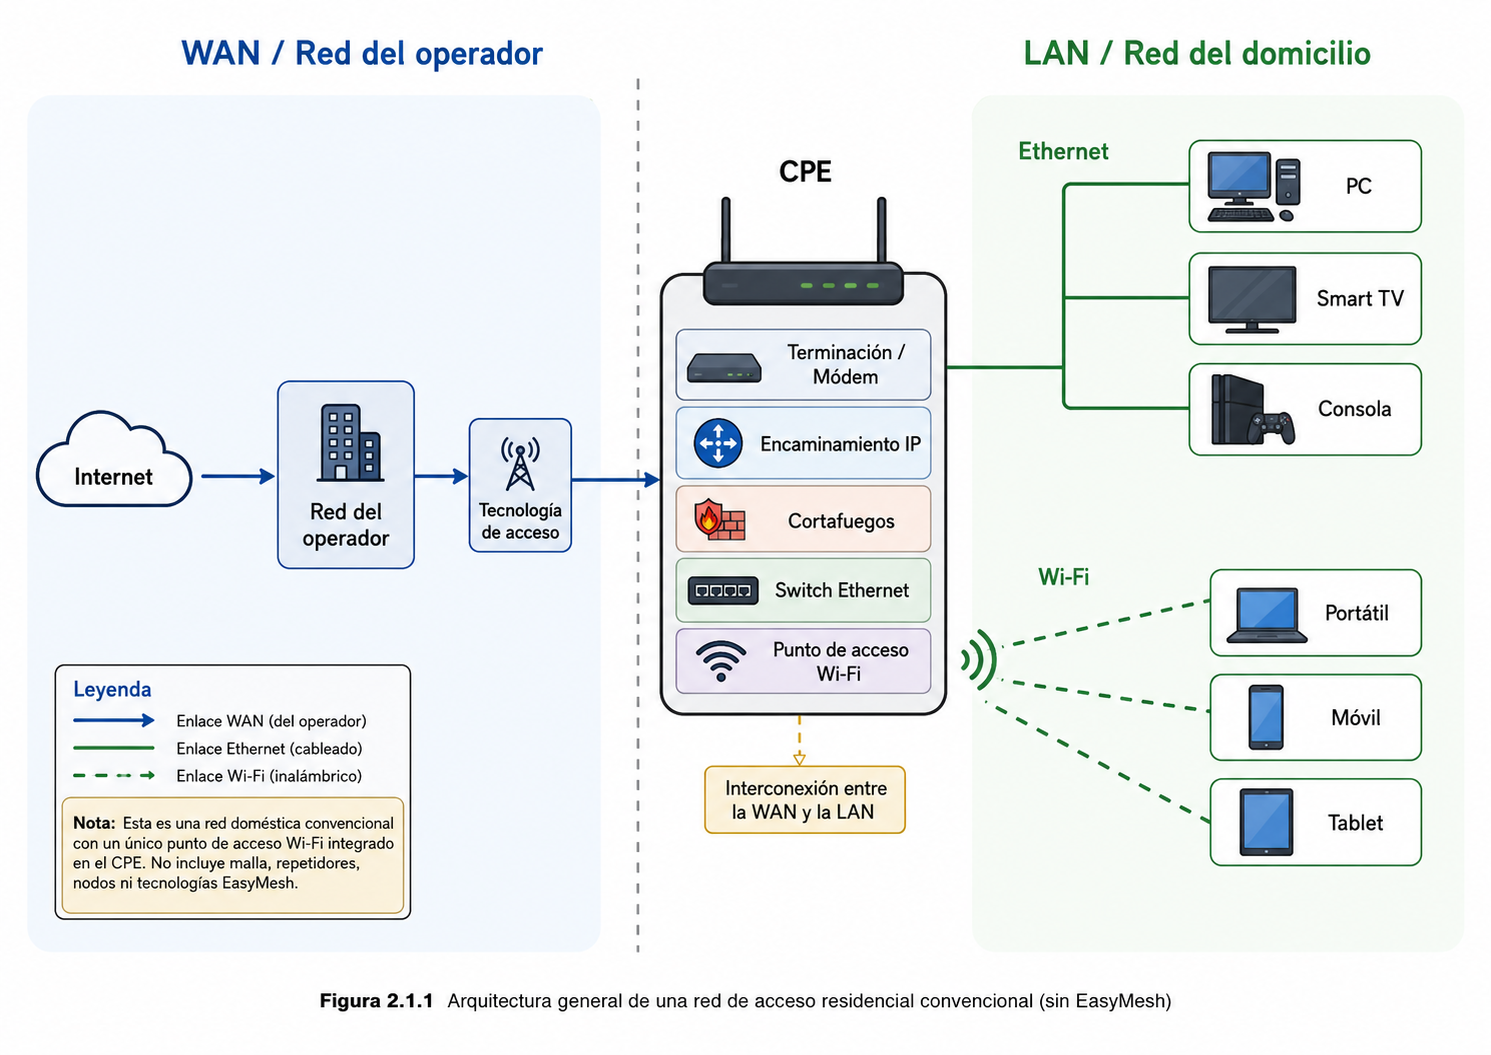
\includegraphics[width=0.90\textwidth]
    {figures/red_acceso_residencial.png}

    \caption[Arquitectura general de una red de acceso residencial.]
    {Arquitectura general de una red de acceso residencial. La red del
    operador proporciona conectividad mediante el enlace WAN, mientras
    que el CPE integra las funciones de terminación, encaminamiento,
    seguridad, conmutación y acceso inalámbrico necesarias para conectar
    los dispositivos de la red LAN.
    \textit{Fuente: imagen generada mediante ChatGPT (OpenAI) a partir
    de las indicaciones de la autora y basada en las arquitecturas
    descritas por Broadband Forum e ITU-T
    \cite{bbf_tr124_i9,itu_g9970}.}}

    \label{fig:red-acceso-residencial}
\end{figure}

La arquitectura representada permite diferenciar el ámbito de
responsabilidad del operador y el ámbito correspondiente a la red
interna. El proveedor administra la infraestructura de acceso y puede
gestionar remotamente el CPE, mientras que el rendimiento de la LAN
también depende de la distribución de los equipos, de los medios
utilizados y de las condiciones particulares del domicilio.

Esta separación resulta importante durante el diagnóstico de
incidencias. Una degradación observada por el usuario puede originarse en
la red del operador, en la interfaz WAN, en el propio CPE, en el segmento
LAN o en el terminal final. Por tanto, comprobar únicamente la
disponibilidad del enlace de acceso no permite determinar necesariamente
el estado completo del servicio.

En el contexto de este proyecto, el CPE adquiere una función adicional,
ya que integra el \textbf{controlador EasyMesh} y constituye el equipo
registrado en la plataforma de gestión. La información relacionada con
los agentes y los clientes conectados a la red mallada debe recopilarse y
exponerse a través de este dispositivo. En consecuencia, el CPE
representa tanto el \textbf{punto de interconexión entre la WAN y la LAN}
como el \textbf{punto principal de observación y gestión de la red
residencial}.

\subsection{Red interna del usuario}
\label{subsec:red-interna-usuario}

La \textbf{red interna del usuario} comprende el conjunto de dispositivos,
interfaces y enlaces situados dentro del domicilio y utilizados para
distribuir la conectividad proporcionada por el operador. Su función
consiste en permitir la comunicación entre los terminales locales y
facilitar su acceso a servicios externos a través del CPE.

Esta red puede estar formada por enlaces cableados, conexiones
inalámbricas o una combinación de ambos. Los enlaces cableados se
implementan habitualmente mediante \textbf{Ethernet}, mientras que la
conectividad inalámbrica se proporciona mediante tecnologías
\textbf{Wi-Fi}. Ambas tecnologías pertenecen a la familia de estándares
IEEE~802, aunque emplean mecanismos físicos y de acceso al medio
diferentes.

Ethernet se encuentra definido por la familia de estándares
\textbf{IEEE~802.3}, que especifica las funciones de la capa física y de
la subcapa de control de acceso al medio utilizadas en las redes locales
cableadas \cite{ieee_8023_2022}. En una red residencial, Ethernet permite
conectar directamente ordenadores, televisores, consolas, sistemas de
almacenamiento, puntos de acceso y otros equipos mediante enlaces
dedicados.

Los enlaces Ethernet proporcionan generalmente una conexión estable y
predecible, ya que cada dispositivo utiliza un medio físico delimitado.
No obstante, el rendimiento efectivo también depende de la velocidad
negociada por las interfaces, de la categoría del cableado, de la
capacidad del conmutador, del procesamiento realizado por el CPE y de la
carga existente en los enlaces compartidos.

La conectividad inalámbrica se basa en la familia de estándares
\textbf{IEEE~802.11}, que define las funciones MAC y PHY de las redes
WLAN (\textit{Wireless Local Area Network})
\cite{ieee_80211_2024}. A diferencia de Ethernet, los dispositivos Wi-Fi
comparten el medio radioeléctrico y deben coordinar el acceso al canal
antes de transmitir.

En una infraestructura Wi-Fi convencional, el
\textbf{punto de acceso o AP}
(\textit{Access Point}) actúa como elemento de conexión entre los
terminales inalámbricos y la red de distribución. Cuando el AP se
encuentra integrado en el CPE, los clientes asociados pueden comunicarse
con la red LAN y acceder a Internet a través de las funciones de
encaminamiento proporcionadas por el propio equipo.

El conjunto formado por un punto de acceso y los clientes asociados
constituye un \textbf{BSS}
(\textit{Basic Service Set}). Este conjunto se identifica mediante un
\textbf{BSSID}
(\textit{Basic Service Set Identifier}), normalmente asociado a una
dirección MAC utilizada por la interfaz radio del punto de acceso. Por
otro lado, el nombre lógico presentado al usuario se denomina
\textbf{SSID}
(\textit{Service Set Identifier}).

El SSID permite identificar una red inalámbrica desde la perspectiva del
usuario, pero no determina por sí solo el punto de acceso concreto que
proporciona conectividad al terminal. Varios puntos de acceso pueden
difundir el mismo SSID y pertenecer a una misma red lógica, aunque cada
uno utilice un BSSID diferente. Esta distinción resulta especialmente
relevante en arquitecturas con varios puntos de acceso y en redes Wi-Fi
Mesh.

La red interna también requiere mecanismos de configuración de red. El
CPE incorpora habitualmente un \textbf{servidor DHCP}
(\textit{Dynamic Host Configuration Protocol}) encargado de asignar a los
clientes parámetros como la dirección IP, la máscara de red, la puerta
de enlace y los servidores DNS. El funcionamiento básico de DHCP se
define en RFC~2131 \cite{rfc2131}.

En redes IPv4 residenciales se utilizan normalmente
\textbf{direcciones privadas}, que no se anuncian directamente en
Internet. RFC~1918 reserva para este propósito los bloques
\texttt{10.0.0.0/8}, \texttt{172.16.0.0/12} y
\texttt{192.168.0.0/16} \cite{rfc1918}. Estas direcciones permiten
identificar los dispositivos dentro de la red local sin consumir
direcciones IPv4 públicas.

Para facilitar el acceso simultáneo de varios dispositivos a Internet,
el CPE aplica habitualmente mecanismos de
\textbf{traducción de direcciones de red o NAT}
(\textit{Network Address Translation}). Mediante este procedimiento, las
direcciones privadas utilizadas en la LAN se traducen a una dirección
válida en la interfaz WAN. De esta forma, varios terminales pueden
compartir la conectividad externa proporcionada por el operador.

La \textbf{puerta de enlace predeterminada} de los terminales suele
corresponder a la dirección IP del CPE dentro de la LAN. Cuando un
dispositivo necesita comunicarse con una dirección que no pertenece a su
red local, entrega el tráfico al CPE para que este determine la ruta
correspondiente y lo reenvíe hacia la interfaz WAN.

La red interna puede incorporar además un
\textbf{conmutador Ethernet}, integrado en el CPE o instalado como un
equipo independiente. El conmutador reenvía las tramas en función de las
direcciones MAC aprendidas en sus puertos y permite ampliar el número de
dispositivos cableados conectados a la misma red local.

Desde el punto de vista lógico, los dispositivos de la vivienda pueden
pertenecer a una única subred o distribuirse entre varias redes
diferenciadas. Algunos CPE permiten separar la red principal, la red de
invitados, los dispositivos IoT y otros servicios mediante distintas
interfaces, identificadores SSID o redes virtuales. Esta separación
puede mejorar el aislamiento y el control del tráfico, aunque su
disponibilidad depende de las funciones proporcionadas por el equipo.

La Figura~\ref{fig:red-interna-usuario} representa los principales
elementos de una red interna residencial convencional. El CPE integra las
funciones de encaminamiento, DHCP, NAT, conmutación Ethernet y acceso
Wi-Fi. Los dispositivos cableados se conectan mediante el conmutador,
mientras que los terminales inalámbricos se asocian al punto de acceso.

\begin{figure}[H]
    \centering
    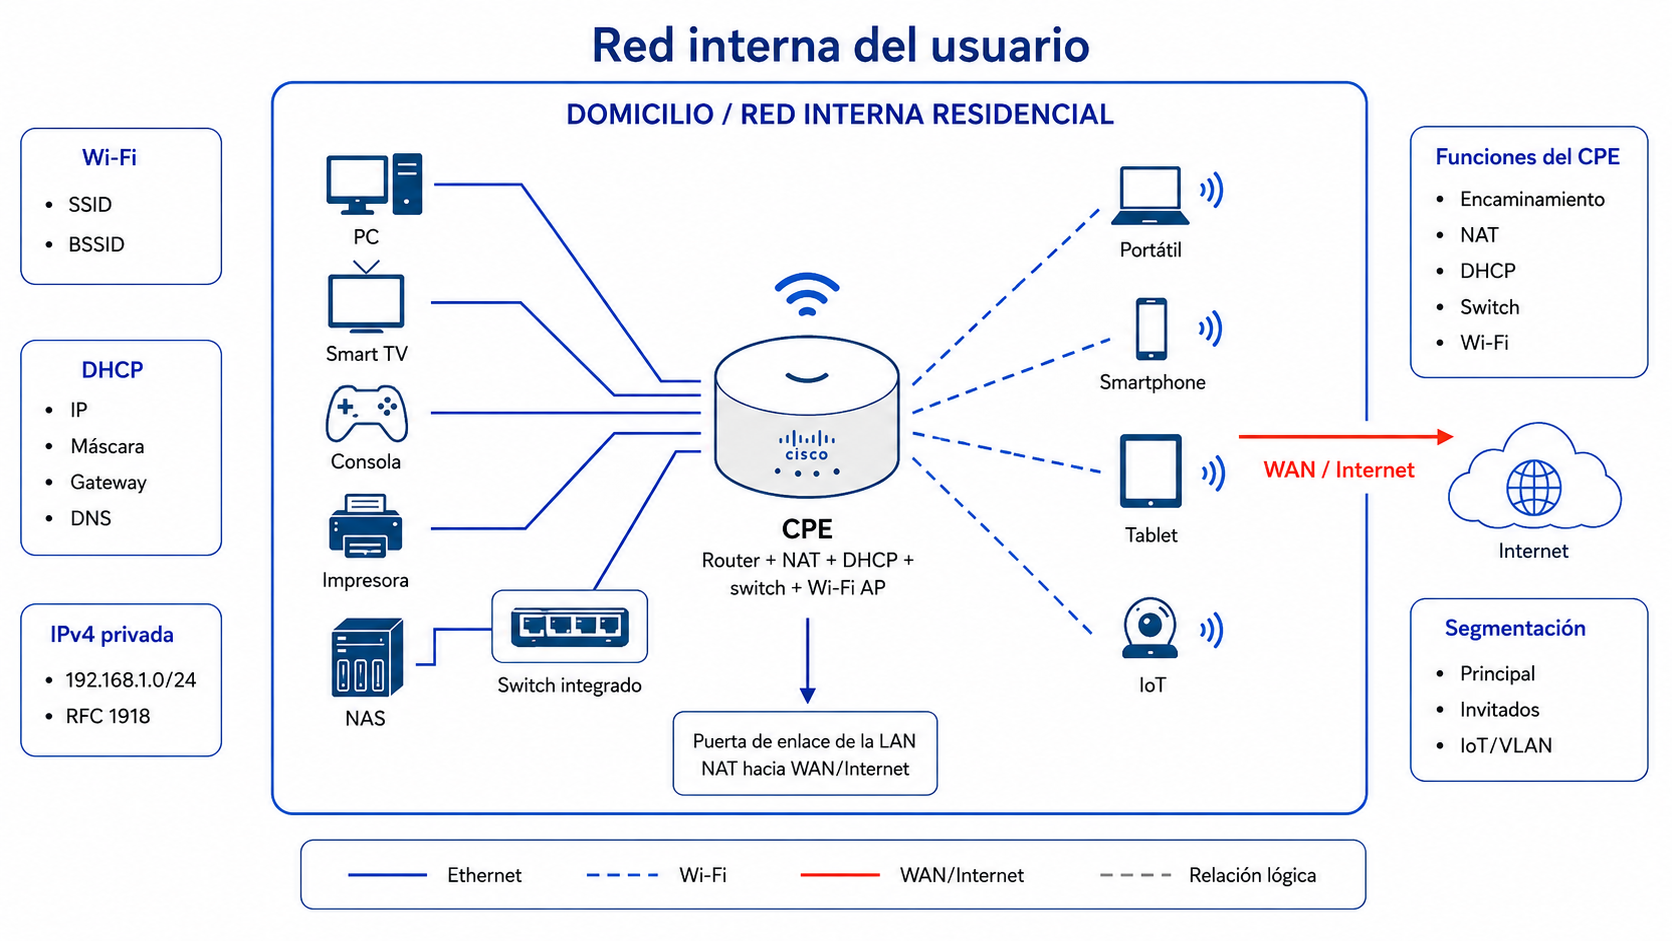
\includegraphics[width=0.90\textwidth]
    {figures/red_interna_usuario.png}

    \caption[Estructura de una red interna residencial convencional.]
    {Estructura de una red interna residencial convencional. El CPE
    integra las funciones de encaminamiento, traducción de direcciones,
    asignación de parámetros IP, conmutación Ethernet y acceso Wi-Fi. Los
    dispositivos finales se conectan mediante enlaces cableados o
    inalámbricos.
    \textit{Fuente: imagen generada mediante ChatGPT (OpenAI) a partir
    de las indicaciones de la autora y basada en las especificaciones
    IEEE~802.3, IEEE~802.11, RFC~1918 y RFC~2131
    \cite{ieee_8023_2022,ieee_80211_2024,rfc1918,rfc2131}.}}

    \label{fig:red-interna-usuario}
\end{figure}

La coexistencia de dispositivos cableados e inalámbricos provoca que el
rendimiento de la red interna dependa de varios segmentos. Un terminal
conectado mediante Ethernet puede disponer de un enlace estable con el
CPE, mientras que un cliente Wi-Fi queda condicionado por la cobertura,
las interferencias, la ocupación del canal y la calidad de su asociación
con el punto de acceso.

Por tanto, la \textbf{conectividad de la LAN no debe interpretarse como
una propiedad uniforme}. Cada cliente puede utilizar una tecnología,
banda de frecuencia, radio, punto de acceso y tasa de enlace diferente.
Estas diferencias deben considerarse al analizar el rendimiento y la
experiencia obtenida por los usuarios.

En el contexto del presente proyecto, esta distinción adquiere una mayor
relevancia porque la red interna no dispone únicamente del punto de
acceso integrado en el CPE. La cobertura se distribuye mediante varios
nodos EasyMesh, por lo que resulta necesario conocer no solo la identidad
del cliente, sino también el \textbf{nodo, el radio y el punto de acceso
que le proporcionan conectividad en cada instante}.

\subsection{Impacto de la cobertura, interferencia y saturación}
\label{subsec:impacto-cobertura-interferencia-saturacion}

El rendimiento de una red Wi-Fi residencial depende de las
\textbf{condiciones radioeléctricas}, de la configuración de los equipos
y de la actividad de los dispositivos que comparten el medio. A
diferencia de una conexión Ethernet, el enlace inalámbrico utiliza un
canal radio compartido y variable, por lo que su comportamiento puede
cambiar incluso cuando la configuración de la red permanece constante.

El Broadband Forum considera la \textbf{cobertura}, la
\textbf{capacidad}, el \textbf{ancho de banda}, la
\textbf{estabilidad} y la \textbf{robustez} como dimensiones relevantes
para evaluar el funcionamiento de los equipos Wi-Fi residenciales
\cite{bbf_tr398_i3c1}. Estas dimensiones están condicionadas por
múltiples factores que pueden actuar de forma simultánea.

Uno de los principales factores es la \textbf{distancia entre el cliente
y el punto de acceso}. La potencia recibida disminuye a medida que
aumenta la separación entre ambos dispositivos. Cuando el nivel de señal
se reduce, el enlace puede utilizar esquemas de modulación y codificación
más robustos, pero con una menor tasa física de transmisión.

La propagación también depende de los
\textbf{obstáculos presentes en el domicilio}. Paredes, techos, puertas,
muebles y estructuras metálicas atenúan o reflejan la señal. La magnitud
de esta atenuación depende del material, del grosor del obstáculo, de la
banda de frecuencia utilizada y de la posición relativa entre el emisor y
el receptor.

La reflexión de las ondas sobre diferentes superficies provoca la
\textbf{propagación multitrayecto}. En este fenómeno, varias versiones de
una misma señal alcanzan el receptor siguiendo recorridos distintos y
con diferentes retardos. Los sistemas Wi-Fi modernos incorporan técnicas
para aprovechar o compensar estos efectos, aunque las condiciones
desfavorables de propagación pueden reducir la estabilidad y la capacidad
del enlace.

La \textbf{banda de frecuencia} utilizada también condiciona la
cobertura. Las bandas con frecuencias más bajas presentan, en general,
una mayor capacidad de propagación y penetración a través de obstáculos.
Las bandas de frecuencia más elevadas pueden ofrecer más canales y mayor
capacidad, pero suelen presentar una menor cobertura efectiva dentro de
la vivienda.

Otro factor relevante es la \textbf{interferencia}. Esta puede proceder
de otras redes Wi-Fi que utilizan canales próximos o coincidentes, de
dispositivos que emplean la misma banda de frecuencia o de fuentes
electromagnéticas externas. La interferencia incrementa la probabilidad
de errores y puede obligar a repetir transmisiones, lo que reduce el
caudal útil disponible.

En un entorno residencial pueden distinguirse dos situaciones. La
\textbf{interferencia cocanal} se produce cuando varias redes utilizan el
mismo canal y deben compartir el tiempo de transmisión. La
\textbf{interferencia de canal adyacente} aparece cuando las emisiones de
canales próximos se solapan y dificultan la recepción correcta de las
tramas.

La selección del \textbf{ancho de canal} también afecta al rendimiento.
Un canal más ancho permite utilizar una mayor cantidad de espectro y
alcanzar tasas físicas superiores. Sin embargo, también incrementa la
probabilidad de solapamiento con otras redes y puede reducir el número de
canales no superpuestos disponibles en el entorno.

La \textbf{ocupación del canal} representa la proporción de tiempo durante
la cual el medio se encuentra ocupado por transmisiones Wi-Fi,
interferencias u otras fuentes detectadas por la radio. Cuando la
ocupación aumenta, los dispositivos deben esperar más tiempo antes de
transmitir, por lo que se incrementa la latencia y se reduce la capacidad
efectiva disponible para cada cliente.

El mecanismo de acceso al medio utilizado por IEEE~802.11 se basa en la
detección del canal antes de transmitir. Como consecuencia, los clientes
asociados a una misma radio compiten por el acceso al medio y comparten
el tiempo disponible. El aumento del número de dispositivos activos puede
provocar una reducción del rendimiento individual, aunque el nivel de
señal de cada cliente sea adecuado.

La \textbf{carga del punto de acceso} depende tanto del número de clientes
asociados como del tráfico generado por cada uno. Un dispositivo que
realiza una transferencia intensiva puede consumir una parte
significativa del tiempo de transmisión disponible y afectar al resto de
los terminales conectados a la misma radio.

Las retransmisiones también influyen en el rendimiento. Cuando una trama
no se recibe correctamente, debe enviarse de nuevo. Un aumento del número
de retransmisiones consume capacidad adicional, incrementa el tiempo
necesario para completar las transferencias y puede provocar variaciones
en la latencia y en el caudal observado.

La \textbf{tasa PHY} representa la velocidad física negociada entre el
cliente y el punto de acceso. Este valor depende de la modulación, la
codificación, el número de flujos espaciales, el ancho de canal y las
condiciones radioeléctricas. No obstante, la tasa PHY no equivale al
caudal útil de la aplicación, ya que no descuenta las cabeceras, los
tiempos de acceso al medio, las retransmisiones ni el tráfico de control.

El rendimiento también puede estar condicionado por el
\textbf{enlace de \textit{backhaul}}. En una red con varios puntos de
acceso, el nodo que proporciona conectividad al cliente debe transportar
el tráfico hasta el equipo principal. Si el \textit{backhaul} presenta
una baja capacidad, una señal deficiente, interferencias o una elevada
ocupación, puede convertirse en el principal cuello de botella de la
comunicación.

En un enlace de \textit{backhaul} inalámbrico, el tráfico del cliente
puede atravesar más de un salto antes de alcanzar el CPE. Cada salto
consume recursos radio y puede añadir retardos, retransmisiones y
variabilidad temporal. Por tanto, una buena conexión entre el cliente y
el punto de acceso no garantiza por sí sola un rendimiento extremo a
extremo adecuado.

Las degradaciones descritas no actúan necesariamente de forma aislada.
Por ejemplo, una señal reducida puede provocar una disminución de la tasa
PHY, un aumento de las retransmisiones y una mayor ocupación del canal.
Del mismo modo, una elevada interferencia puede afectar simultáneamente
al enlace del cliente y al \textit{backhaul} inalámbrico.

Por esta razón, el diagnóstico no debe basarse en una única métrica. La
evaluación requiere \textbf{correlacionar el nivel de señal, la tasa PHY,
la utilización del canal, las retransmisiones, la asociación del cliente
y el estado del \textit{backhaul}}. Esta correlación permite distinguir
entre una degradación localizada en el enlace de acceso del cliente y una
limitación que afecta a otro segmento de la red.

Además, los efectos de estas degradaciones se reflejan en indicadores
extremo a extremo. Una menor capacidad disponible puede reducir el
caudal, mientras que la contención, las retransmisiones y la congestión
pueden incrementar la latencia, el \textit{jitter} y la pérdida de
paquetes. Estos parámetros se utilizan habitualmente para caracterizar el
rendimiento de una comunicación y su impacto sobre aplicaciones
interactivas o multimedia \cite{itu_y1545}.

En el contexto del presente proyecto, estos factores justifican la
necesidad de recopilar métricas tanto del cliente como del nodo EasyMesh
que le proporciona servicio. La información debe permitir identificar si
la degradación se relaciona con la cobertura, la radio, la carga, el
enlace de \textit{backhaul} o la propia actualización de la telemetría.

\subsection{Diferencia entre QoS y QoE}
\label{subsec:diferencia-qos-qoe}

La evaluación del funcionamiento de una red residencial requiere
diferenciar entre la \textbf{calidad técnica proporcionada por la
infraestructura} y la \textbf{experiencia obtenida por el usuario durante
la utilización de un servicio}. Estos dos ámbitos se representan
mediante los conceptos de calidad de servicio y calidad de experiencia.

La \textbf{calidad de servicio o QoS}
(\textit{Quality of Service}) describe las prestaciones técnicas
proporcionadas por una red o servicio de telecomunicaciones. La
recomendación ITU-T E.800 establece un marco común para definir y evaluar
la QoS desde las perspectivas del usuario, del proveedor, del fabricante
y de los organismos reguladores \cite{itu_e800}.

En una red Wi-Fi residencial, la QoS puede caracterizarse mediante
\textbf{indicadores objetivos y cuantificables}. Entre ellos se
encuentran el caudal de transferencia, la latencia, la variación de la
latencia, la pérdida de paquetes, la disponibilidad, la tasa física del
enlace, el nivel de señal, la utilización del canal y el número de
retransmisiones.

El \textbf{caudal} representa la cantidad de información útil que puede
transmitirse durante un intervalo de tiempo. Aunque suele expresarse en
bits por segundo, su valor no debe confundirse con la tasa PHY negociada
entre el cliente y el punto de acceso. El caudal útil es inferior porque
la comunicación incorpora cabeceras, mensajes de control, tiempos de
espera, confirmaciones y posibles retransmisiones.

La \textbf{latencia} representa el tiempo necesario para que la
información viaje entre dos puntos de la comunicación. En redes
residenciales suele evaluarse mediante el tiempo de ida y vuelta o RTT
(\textit{Round-Trip Time}). Este indicador resulta especialmente
relevante en aplicaciones interactivas, como videoconferencias,
videojuegos en línea, telefonía IP y acceso remoto.

El \textbf{\textit{jitter}} describe la variación temporal de la
latencia entre paquetes sucesivos. Una latencia media moderada puede
resultar aceptable si permanece estable, mientras que una variación
elevada puede provocar interrupciones, desincronización o la necesidad de
utilizar búferes adicionales en aplicaciones de voz y vídeo.

La \textbf{pérdida de paquetes} representa la proporción de unidades de
información que no alcanzan correctamente su destino. La pérdida puede
producirse por interferencias, errores radioeléctricos, congestión,
desbordamiento de colas o fallos en alguno de los enlaces atravesados.
Dependiendo del protocolo utilizado, los paquetes perdidos pueden
retransmitirse o producir una degradación directamente visible para la
aplicación.

La \textbf{disponibilidad} indica si el servicio o el dispositivo se
encuentran accesibles durante un periodo determinado. En el contexto de
una red residencial, la falta de disponibilidad puede deberse a la
pérdida de conectividad WAN, a un fallo del CPE, a la indisponibilidad de
un agente, a la desconexión del cliente o a una interrupción temporal
durante un proceso de movilidad.

Estas métricas permiten describir el comportamiento técnico de la red,
pero no representan de forma completa la percepción del usuario. Por
este motivo, se utiliza el concepto de
\textbf{calidad de experiencia o QoE}
(\textit{Quality of Experience}), que incorpora el resultado percibido
durante la utilización de una aplicación o servicio
\cite{itu_p10_g100}.

La QoE depende de factores técnicos, humanos y contextuales. Entre los
factores técnicos se encuentran el caudal disponible, la latencia, la
pérdida de paquetes, la resolución multimedia y el tiempo de respuesta de
la aplicación. Los factores humanos incluyen las expectativas, la
experiencia previa y la sensibilidad del usuario. Los factores
contextuales comprenden el tipo de terminal, el entorno de uso, la
aplicación utilizada y la finalidad de la comunicación.

Por tanto, una misma condición de red puede producir experiencias
distintas. Una latencia elevada puede tener un efecto limitado durante
la descarga de un archivo, pero resultar claramente perceptible en una
videollamada o en un videojuego interactivo. De forma similar, una
reducción temporal del caudal puede pasar inadvertida durante la
navegación web y provocar interrupciones durante la reproducción de
vídeo de alta resolución.

La relación entre QoS y QoE no es lineal ni uniforme. Una degradación
técnica no produce necesariamente una degradación perceptible inmediata,
ya que las aplicaciones pueden incorporar mecanismos de adaptación,
almacenamiento en búfer, corrección de errores o modificación dinámica de
la calidad. Del mismo modo, una experiencia insatisfactoria puede estar
provocada por el servidor, la aplicación o el terminal, aunque la red
residencial presente valores técnicos adecuados.

En este proyecto, la QoE no se determina mediante encuestas subjetivas,
sino mediante \textbf{medidas activas ejecutadas desde el terminal}. Estas
medidas permiten obtener indicadores objetivos relacionados con la
experiencia, como el caudal de descarga y subida, la latencia, el
\textit{jitter}, la pérdida de paquetes y el comportamiento bajo carga.

Estas pruebas deben interpretarse como
\textbf{indicadores objetivos asociados a la experiencia} y no como una
evaluación subjetiva completa. La percepción real también depende de la
aplicación, del contenido, del terminal y de las expectativas del
usuario. No obstante, las medidas activas permiten comparar escenarios
bajo condiciones reproducibles y relacionar el comportamiento extremo a
extremo con la telemetría de la red.

La Figura~\ref{fig:relacion-qos-qoe} representa la relación general entre
las condiciones técnicas de la infraestructura, las métricas de QoS, el
comportamiento de las aplicaciones y la experiencia obtenida por el
usuario.

\begin{figure}[H]
    \centering
    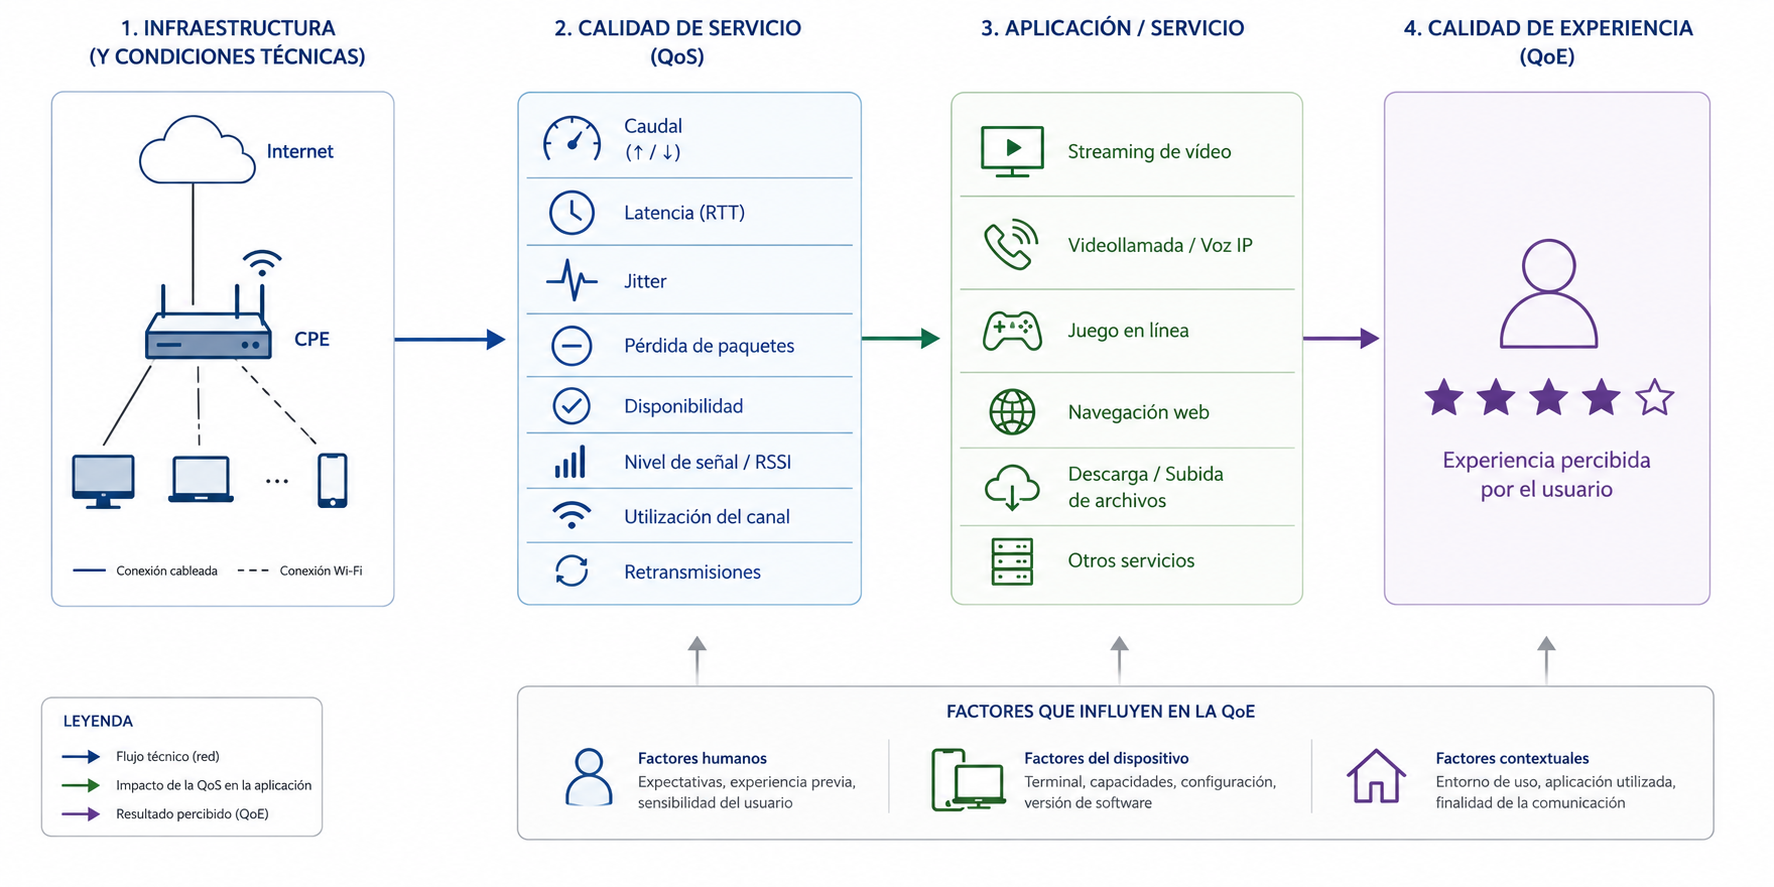
\includegraphics[width=0.90\textwidth]
    {figures/relacion_qos_qoe.png}

    \caption[Relación entre calidad de servicio y calidad de experiencia.]
    {Relación entre la calidad de servicio y la calidad de experiencia.
    Las condiciones técnicas de la red se reflejan en métricas objetivas
    de QoS, cuyo efecto sobre la experiencia depende de la aplicación,
    del terminal y del contexto de uso.
    \textit{Fuente: imagen generada mediante ChatGPT (OpenAI) a partir
    de las indicaciones de la autora y basada en las definiciones de las
    recomendaciones ITU-T E.800 y P.10/G.100
    \cite{itu_e800,itu_p10_g100}.}}

    \label{fig:relacion-qos-qoe}
\end{figure}

En el contexto de una red EasyMesh, la interpretación conjunta de QoS y
QoE requiere conocer el \textbf{nodo de asociación del cliente}, la
calidad del enlace radio, el estado del \textit{backhaul} y la antigüedad
de la telemetría. Sin esta información, una degradación observada desde el
terminal no puede relacionarse de forma fiable con el elemento de la red
que la origina.

Por esta razón, la plataforma desarrollada combina
\textbf{telemetría obtenida desde el CPE y la infraestructura EasyMesh}
con \textbf{medidas activas realizadas desde el terminal móvil}. La
correlación temporal de ambas fuentes permite analizar si una variación
de la experiencia coincide con cambios de asociación, disminuciones de
la señal, limitaciones de capacidad, interrupciones de conectividad o
degradaciones del enlace de \textit{backhaul}.

En consecuencia, la QoS proporciona la
\textbf{visión técnica del funcionamiento de la red}, mientras que las
medidas relacionadas con la QoE permiten aproximar el
\textbf{resultado experimentado por el usuario}. El análisis conjunto de
ambas dimensiones constituye uno de los fundamentos de la plataforma de
monitorización propuesta.

\section{Redes WiFi Mesh}
\label{sec:redes-wifi-mesh}

La cobertura proporcionada por un único punto de acceso puede resultar
insuficiente en viviendas con varias plantas, superficies amplias,
obstáculos constructivos o zonas alejadas del CPE. En estas condiciones,
el nivel de señal disminuye y el enlace inalámbrico puede experimentar
una reducción de la tasa física, un aumento de las retransmisiones y una
degradación del caudal disponible.

Una solución convencional consiste en incorporar
\textbf{puntos de acceso adicionales} o repetidores inalámbricos. Sin
embargo, cuando estos equipos funcionan de manera independiente, cada
uno puede requerir una configuración específica y proporcionar una
visión fragmentada de la red. Esta situación dificulta la coordinación
de las radios, la selección del punto de acceso y el seguimiento de los
clientes durante sus desplazamientos.

Las \textbf{redes Wi-Fi Mesh} permiten ampliar la cobertura mediante la
cooperación de varios nodos distribuidos dentro del domicilio. Estos
nodos forman una única infraestructura lógica y proporcionan
conectividad a los dispositivos finales desde diferentes ubicaciones. La
red puede adaptar la trayectoria seguida por el tráfico y mantener el
servicio cuando el cliente se desplaza entre las distintas zonas de
cobertura.

En una arquitectura Mesh se distinguen dos tipos principales de
conexiones. El \textbf{enlace de acceso o \textit{fronthaul}} conecta los
clientes Wi-Fi con el nodo que les proporciona servicio. Por otra parte,
el \textbf{enlace de \textit{backhaul}} conecta los nodos de la red entre
sí y permite transportar el tráfico hacia el equipo principal o hacia la
red del operador.

El \textit{backhaul} puede establecerse mediante Ethernet o de forma
inalámbrica. Un \textit{backhaul} cableado proporciona normalmente una
mayor estabilidad y evita utilizar recursos radio para transportar el
tráfico entre nodos. En cambio, el \textit{backhaul} inalámbrico facilita
el despliegue cuando no existe cableado disponible, aunque comparte el
medio radioeléctrico y puede verse afectado por la distancia, los
obstáculos, la interferencia y la ocupación del canal.

La utilización de varios puntos de acceso introduce además la necesidad
de coordinar la configuración de la red. Los nodos deben compartir
información sobre las radios, los canales, los clientes asociados, la
calidad de los enlaces y la topología disponible. Esta coordinación
permite aplicar mecanismos de selección de canal, gestión de potencia,
balanceo de carga y orientación de clientes hacia el punto de acceso más
adecuado.

Dentro de este ámbito, \textbf{Wi-Fi EasyMesh} define una arquitectura
interoperable para redes Wi-Fi formadas por varios puntos de acceso. La
especificación establece una organización basada en un
\textbf{controlador} y uno o varios \textbf{agentes}, así como los
mecanismos empleados para intercambiar información y coordinar el
funcionamiento de la red Multi-AP
\cite{wifi_alliance_easymesh}.

El \textbf{controlador EasyMesh} constituye la entidad lógica encargada
de coordinar la red. Entre sus funciones se encuentran la obtención de la
topología, la recopilación de información sobre los agentes, la
configuración de determinados parámetros y la toma de decisiones
relacionadas con la gestión de los clientes y de los recursos radio.

Los \textbf{agentes EasyMesh} se encuentran distribuidos en diferentes
ubicaciones del domicilio y proporcionan conectividad Wi-Fi a los
terminales. Cada agente puede disponer de una o varias radios, varios
puntos de acceso y uno o más enlaces de \textit{backhaul}. Los agentes
intercambian información con el controlador para mantener una visión
coordinada de la red.

La arquitectura EasyMesh se apoya en los mecanismos definidos por
\textbf{IEEE~1905.1}, que proporciona una capa de abstracción para redes
domésticas formadas por diferentes tecnologías de enlace. Este estándar
permite descubrir los dispositivos, representar la topología e
intercambiar mensajes de control entre los nodos que forman la
infraestructura Multi-AP \cite{ieee_1905_1}.

Desde la perspectiva del usuario, la red puede presentar un mismo
\textbf{SSID} en diferentes puntos de acceso. De esta forma, el terminal
percibe una única red lógica aunque la cobertura sea proporcionada por
varios nodos. Cada punto de acceso utiliza su propio BSSID, lo que permite
identificar de manera específica la radio y la interfaz con las que se
encuentra asociado el cliente.

Cuando el terminal se desplaza por el domicilio, puede cambiar su
asociación desde un punto de acceso hacia otro. Este proceso se relaciona
con el \textbf{\textit{roaming}} y puede estar apoyado por mecanismos de
\textit{client steering}. No obstante, la decisión final de asociación
también depende del comportamiento y de las capacidades implementadas por
el propio dispositivo cliente.

La Figura~\ref{fig:arquitectura-mesh-general} representa de forma
simplificada una red Wi-Fi Mesh residencial. El controlador se encuentra
integrado en el nodo principal, mientras que los agentes amplían la
cobertura y transportan el tráfico de los clientes mediante enlaces de
\textit{backhaul}.

\begin{figure}[H]
    \centering
    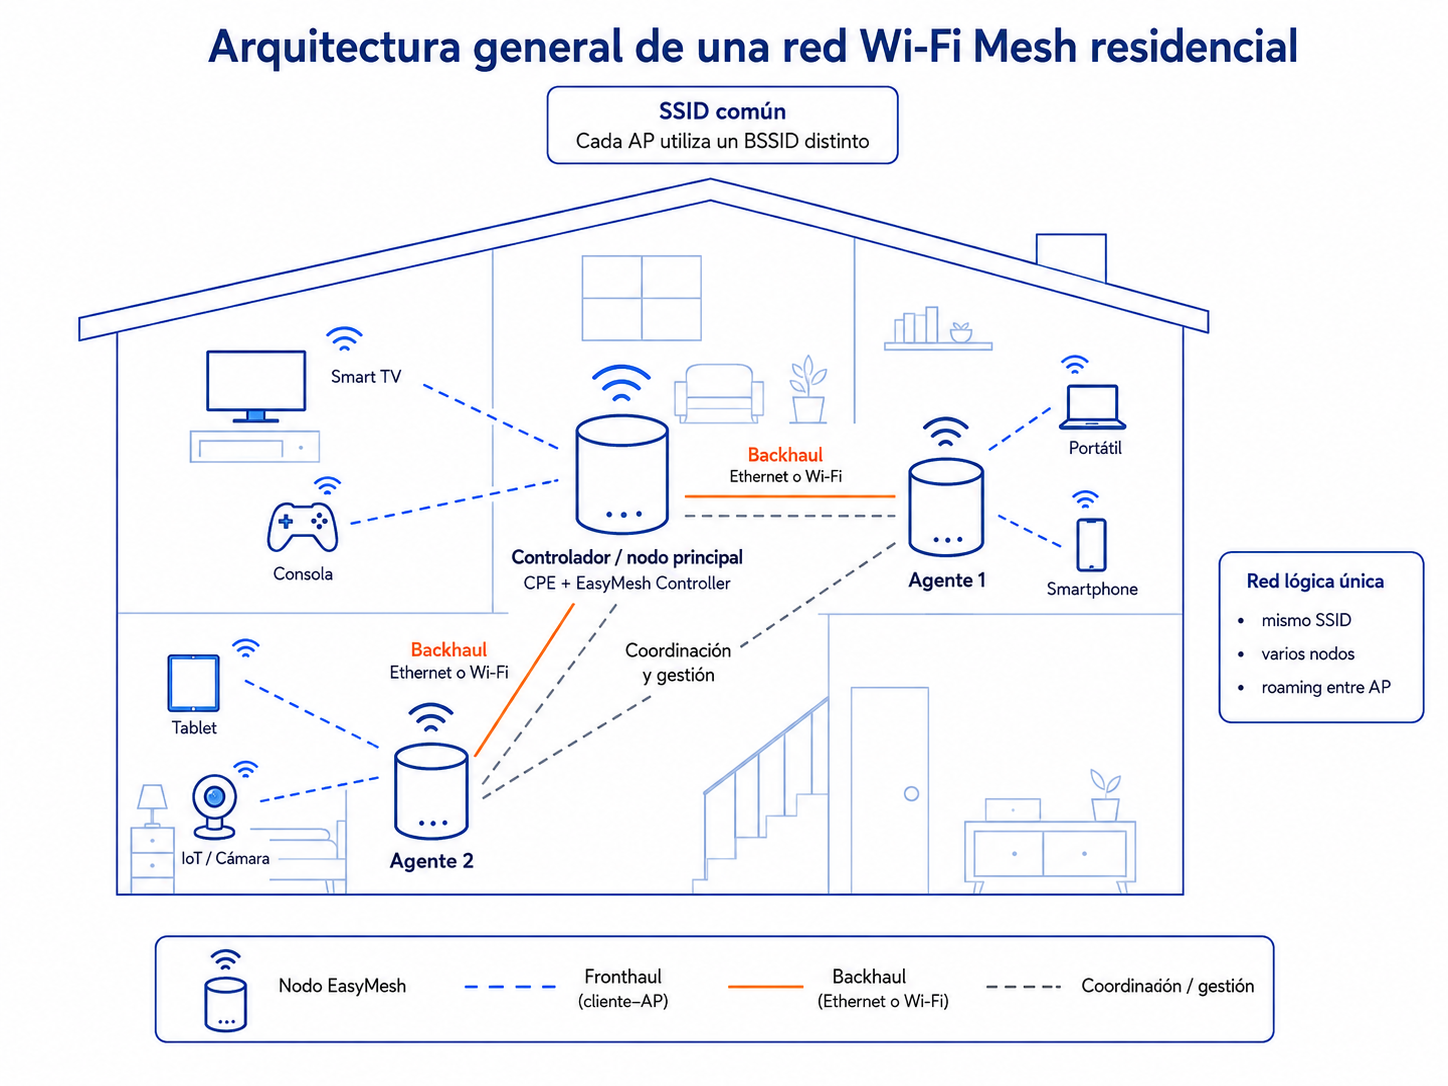
\includegraphics[width=0.90\textwidth]
    {figures/arquitectura_mesh_general.png}

    \caption[Arquitectura general de una red Wi-Fi Mesh residencial.]
    {Arquitectura general de una red Wi-Fi Mesh residencial. El
    controlador coordina los agentes distribuidos en el domicilio,
    mientras que los clientes se conectan mediante enlaces de acceso y
    el tráfico se transporta entre los nodos a través de enlaces de
    \textit{backhaul}.
    \textit{Fuente: imagen generada mediante ChatGPT (OpenAI) a partir
    de las indicaciones de la autora y basada en la especificación
    Wi-Fi EasyMesh y en IEEE~1905.1
    \cite{wifi_alliance_easymesh,ieee_1905_1}.}}

    \label{fig:arquitectura-mesh-general}
\end{figure}

La introducción de una arquitectura Mesh mejora la cobertura, pero
también incrementa la complejidad de la monitorización. La información
necesaria para caracterizar la conexión de un cliente ya no se encuentra
asociada únicamente al punto de acceso integrado en el CPE, sino que
puede corresponder a cualquiera de los agentes distribuidos en la red.

Por este motivo, la plataforma de gestión debe conocer la
\textbf{topología EasyMesh}, el \textbf{nodo de asociación del cliente},
la radio utilizada, el punto de acceso correspondiente y el estado del
enlace de \textit{backhaul}. La ausencia o la actualización tardía de
esta información puede producir una visión incompleta del servicio y
dificultar el diagnóstico de las degradaciones.

En el laboratorio desarrollado, el controlador EasyMesh se encuentra
integrado en el CPE y constituye el equipo gestionado mediante
TR-069/CWMP. Los agentes no se registran de forma independiente en el
ACS, por lo que la información relacionada con la topología, los nodos y
los clientes debe recopilarse y exponerse a través del controlador.

\subsection{Concepto de red mallada}
\label{subsec:concepto-red-mallada}

Una \textbf{red mallada} o red \textit{Mesh} está formada por varios
nodos de comunicación que cooperan para proporcionar conectividad dentro
de una misma infraestructura. A diferencia de una red inalámbrica
convencional, en la que todos los clientes dependen de un único punto de
acceso, una red mallada distribuye la cobertura entre varios equipos
situados en diferentes ubicaciones.

El objetivo principal de esta arquitectura consiste en
\textbf{ampliar la cobertura inalámbrica} y reducir las zonas en las que
la señal proporcionada por el nodo principal resulta insuficiente. Cada
nodo puede atender a los clientes que se encuentran dentro de su área de
cobertura y transportar posteriormente el tráfico hacia el equipo que
proporciona acceso a la red externa.

Desde la perspectiva del usuario, los distintos nodos pueden formar una
\textbf{única red lógica}. De este modo, los terminales visualizan un
mismo nombre de red y pueden mantener la conectividad mientras se
desplazan por el domicilio, aunque el punto de acceso que les proporciona
servicio cambie durante el recorrido.

La utilización de una red lógica común no implica que todos los nodos
sean equivalentes desde el punto de vista físico. Cada equipo dispone de
sus propias interfaces, radios y puntos de acceso, y cada interfaz
inalámbrica utiliza un identificador específico. Por tanto, aunque el
usuario perciba una única red, la infraestructura está formada por
\textbf{varios enlaces y puntos de asociación diferenciados}.

Los nodos de una red mallada deben disponer de algún mecanismo de
interconexión que permita transportar el tráfico entre ellos. Esta
interconexión puede establecerse mediante enlaces Ethernet, enlaces
inalámbricos o una combinación de ambos. La disponibilidad y la calidad
de estos enlaces condicionan el rendimiento extremo a extremo obtenido
por los clientes.

La topología formada por los nodos no tiene que corresponder
necesariamente a una malla completa. En una
\textbf{topología en estrella}, los nodos secundarios mantienen una
conexión directa con el equipo principal. En una
\textbf{topología en cascada}, un nodo puede alcanzar el equipo principal
a través de otro nodo intermedio. También pueden existir topologías
híbridas en las que se combinan conexiones directas e indirectas.

En una topología en estrella, el tráfico de cada nodo secundario alcanza
directamente el nodo principal. Esta disposición reduce el número de
saltos, pero requiere que todos los nodos dispongan de un enlace
suficientemente estable con el equipo central.

En una topología en cascada, el tráfico puede atravesar varios nodos antes
de alcanzar la salida de la red. Esta configuración permite extender la
cobertura hacia zonas más alejadas, aunque cada salto adicional puede
introducir una reducción de la capacidad disponible, un aumento de la
latencia y una mayor dependencia del estado de los enlaces intermedios.

Una red mallada también requiere mecanismos de
\textbf{coordinación entre los nodos}. La infraestructura debe conocer
los equipos disponibles, las interfaces que los conectan, la calidad de
los enlaces y los clientes asociados. Esta información permite mantener
la topología y adoptar decisiones relacionadas con la configuración y el
funcionamiento de la red.

La coordinación diferencia una red mallada de una instalación formada
únicamente por varios repetidores independientes. Un repetidor
convencional amplía la cobertura de una señal existente, pero puede
carecer de mecanismos comunes para intercambiar información sobre la
topología, gestionar las radios o mantener una visión conjunta de los
clientes.

En una red mallada coordinada, los nodos forman parte de una
\textbf{infraestructura administrada de manera conjunta}. Esta
coordinación permite reducir la fragmentación de la configuración y
facilita funciones como la distribución de la cobertura, la selección de
canales, el seguimiento de los clientes y la adaptación de la topología.

No obstante, una arquitectura Mesh no garantiza por sí sola una mejora
uniforme del rendimiento. La experiencia obtenida depende de la
ubicación de los nodos, de la calidad de sus enlaces, de la ocupación del
medio radioeléctrico, del número de saltos y de la carga soportada por
cada punto de acceso. Una distribución inadecuada puede ampliar la
cobertura sin proporcionar una capacidad suficiente.

Desde el punto de vista de la monitorización, la incorporación de varios
nodos aumenta la cantidad de información necesaria para caracterizar la
conexión. Ya no basta con determinar que un cliente pertenece a la red,
sino que también es necesario conocer el
\textbf{nodo que le proporciona servicio}, el enlace utilizado y la
trayectoria seguida por su tráfico.

En el ámbito residencial, estas funciones de coordinación pueden
implementarse mediante arquitecturas Multi-AP como
\textbf{Wi-Fi EasyMesh} \cite{wifi_alliance_easymesh}. EasyMesh concreta
las entidades y los procedimientos utilizados para organizar los nodos,
intercambiar información y administrar de forma coordinada la red
inalámbrica.

\subsection{Gateway, satélites y clientes WiFi}
\label{subsec:gateway-satelites-clientes-wifi}

En una red Wi-Fi Mesh residencial pueden distinguirse tres tipos de
elementos principales: el \textbf{\textit{gateway} o nodo principal}, los
\textbf{satélites o nodos secundarios} y los
\textbf{clientes Wi-Fi}. Cada uno desempeña una función diferente dentro
de la infraestructura y participa de distinta forma en el transporte del
tráfico.

El \textbf{\textit{gateway}} constituye el punto de interconexión entre
la red interna del domicilio y la red de acceso del operador. Este
elemento se encuentra normalmente integrado en el CPE y concentra
funciones como el encaminamiento IP, la traducción de direcciones, la
asignación de parámetros de red, la protección mediante cortafuegos y el
acceso inalámbrico \cite{bbf_tr124_i9}.

Desde el punto de vista del tráfico, el \textit{gateway} proporciona la
\textbf{salida de la red residencial hacia la interfaz WAN}. Los paquetes
generados por los dispositivos de la vivienda atraviesan este equipo
cuando su destino se encuentra fuera de la red local. Por tanto, el
\textit{gateway} actúa como puerta de enlace predeterminada de los
terminales y como punto de comunicación con los servicios externos.

El \textit{gateway} también puede incorporar uno o varios puntos de
acceso Wi-Fi. En este caso, los clientes situados dentro de su zona de
cobertura pueden asociarse directamente al nodo principal, sin necesidad
de utilizar un nodo intermedio para alcanzar la red local.

Los \textbf{satélites} son nodos secundarios distribuidos en diferentes
ubicaciones del domicilio con el objetivo de ampliar la cobertura de la
red inalámbrica. Cada satélite puede incorporar una o varias radios y
proporcionar uno o varios puntos de acceso a los clientes situados en su
zona de cobertura.

A diferencia del \textit{gateway}, un satélite no constituye normalmente
el punto de salida hacia la red del operador. El tráfico recibido desde
sus clientes debe transportarse hasta el nodo principal, directamente o
a través de otro nodo intermedio. Para clientes debe transportarse hasta el nodo principal, ello, el satélite mantiene un
\textbf{enlace de interconexión con el resto de la red mallada}.

Cuando un satélite se conecta directamente al \textit{gateway}, ambos
forman una estructura próxima a una topología en estrella. Cuando el
satélite utiliza otro nodo secundario para alcanzar el
\textit{gateway}, la trayectoria adopta una disposición en cascada. La
segunda configuración permite ampliar la cobertura hacia zonas más
alejadas, aunque introduce un mayor número de saltos.

Los satélites pueden conectarse mediante
\textbf{enlaces Ethernet} o mediante \textbf{enlaces inalámbricos}. La
interconexión cableada proporciona un medio dedicado y evita utilizar
capacidad radio para transportar el tráfico entre nodos. La conexión
inalámbrica facilita la instalación, pero queda condicionada por la
distancia, los obstáculos, la interferencia y la ocupación del canal.

El término \textbf{satélite} se utiliza habitualmente para describir el
equipo físico secundario de una red Mesh residencial. No obstante, no
debe confundirse automáticamente con las entidades lógicas definidas por
EasyMesh. En dicha arquitectura, las funciones de coordinación y
ejecución se representan formalmente mediante un
\textbf{controlador} y uno o varios \textbf{agentes}
\cite{wifi_alliance_easymesh}.

De manera similar, el término \textit{gateway} describe principalmente
la función de interconexión con la red WAN, mientras que
\textit{controlador EasyMesh} identifica una función lógica de
coordinación. Ambas funciones pueden encontrarse integradas en el mismo
dispositivo físico, como ocurre en el laboratorio desarrollado, pero
representan conceptos distintos.

Los \textbf{clientes Wi-Fi} son los terminales que utilizan la
infraestructura inalámbrica para acceder a la red local y a los servicios
externos. Entre ellos se encuentran teléfonos móviles, ordenadores
portátiles, tabletas, televisores, consolas, cámaras, sensores y otros
dispositivos conectados.

En la terminología de IEEE~802.11, un cliente inalámbrico se representa
mediante una \textbf{estación o STA} (\textit{Station}). El cliente
establece una asociación con un punto de acceso y utiliza las funciones
MAC y PHY definidas por IEEE~802.11 para intercambiar información a
través del medio radioeléctrico \cite{ieee_80211_2024}.

El punto de acceso y las estaciones asociadas forman un
\textbf{BSS} (\textit{Basic Service Set}). El punto de acceso concreto se
identifica mediante su \textbf{BSSID}, mientras que el
\textbf{SSID} representa el nombre lógico de la red presentado al
usuario. En una red mallada, varios nodos pueden anunciar el mismo SSID,
aunque cada punto de acceso mantenga un BSSID diferente.

Esta diferencia permite que el usuario perciba una única red lógica,
mientras que la infraestructura distingue el nodo, la radio y el punto
de acceso que atienden al cliente. Por tanto, conocer únicamente el SSID
no permite determinar desde qué elemento de la red se proporciona la
conectividad.

Los clientes Wi-Fi no presentan necesariamente las mismas capacidades.
Cada terminal puede admitir diferentes generaciones de IEEE~802.11,
bandas de frecuencia, anchos de canal, esquemas de modulación, números de
flujos espaciales y mecanismos de movilidad. Estas diferencias influyen
en la tasa física negociada y en el rendimiento obtenido por cada
dispositivo.

La elección del punto de acceso tampoco depende exclusivamente de la
distancia. El nivel de señal, la calidad del enlace, las capacidades del
terminal, la carga de las radios y los mecanismos de gestión de la red
pueden influir en la asociación. Sin embargo, el cliente conserva un
papel relevante en la decisión final de conexión.

Como se representa en la
Figura~\ref{fig:arquitectura-mesh-general}, el
\textit{gateway} proporciona la conexión con la red externa, los
satélites amplían la cobertura y los clientes se asocian al punto de
acceso disponible en cada zona. El tráfico de un cliente conectado a un
satélite debe recorrer posteriormente la infraestructura mallada hasta
alcanzar el nodo principal.

Desde el punto de vista de la monitorización, resulta necesario
\textbf{diferenciar la identidad del cliente de la identidad del nodo que
le proporciona servicio}. Un mismo terminal puede permanecer conectado a
la misma red lógica y aparecer asociado sucesivamente al
\textit{gateway} o a diferentes satélites.

Por esta razón, la observabilidad de una red Mesh requiere mantener una
relación temporal entre el \textbf{cliente}, el \textbf{punto de acceso},
la \textbf{radio} y el \textbf{nodo físico}. Esta asociación permite
interpretar correctamente las métricas y determinar en qué segmento de
la red puede originarse una degradación.

\subsection{Fronthaul y backhaul}
\label{subsec:fronthaul-backhaul}

En una red Wi-Fi Mesh deben diferenciarse los enlaces utilizados para
proporcionar conectividad a los terminales de aquellos que permiten
interconectar los nodos de la infraestructura. Esta separación se
representa mediante los conceptos de \textbf{\textit{fronthaul}} y
\textbf{\textit{backhaul}}.

El \textbf{\textit{fronthaul}} corresponde al enlace de acceso
establecido entre un \textbf{cliente Wi-Fi} y el punto de acceso al que
se encuentra asociado. A través de este enlace se transportan las tramas
intercambiadas entre el terminal y la infraestructura inalámbrica. Su
funcionamiento se basa en los mecanismos MAC y PHY definidos por la
familia de estándares IEEE~802.11 \cite{ieee_80211_2024}.

El enlace de \textit{fronthaul} queda condicionado por la distancia entre
el cliente y el punto de acceso, la presencia de obstáculos, la banda de
frecuencia, el ancho de canal, la potencia recibida, las interferencias,
la ocupación del medio y las capacidades implementadas por ambos
dispositivos. Estos factores determinan la modulación, la codificación,
el número de flujos espaciales y la tasa física utilizada durante la
comunicación.

Desde el punto de vista del cliente, el \textit{fronthaul} representa el
\textbf{primer tramo inalámbrico de la comunicación}. Una degradación en
este enlace puede manifestarse mediante una disminución de la tasa PHY,
un incremento de las retransmisiones, una mayor latencia o una reducción
del caudal útil obtenido por la aplicación.

Cada cliente establece su enlace de \textit{fronthaul} con un punto de
acceso concreto. Aunque varios puntos de acceso anuncien el mismo SSID,
cada uno utiliza su propio BSSID. Por tanto, para conocer el origen de la
conectividad no basta con identificar el nombre lógico de la red, sino
que es necesario determinar el \textbf{BSSID, la radio y el nodo} a los
que se encuentra asociado el terminal.

Por otra parte, el \textbf{\textit{backhaul}} corresponde al enlace o
conjunto de enlaces utilizados para interconectar los nodos de la red
mallada. Su función consiste en transportar el tráfico recibido por los
satélites hasta el \textit{gateway} o nodo principal, desde el que puede
alcanzar la red local cableada o la interfaz WAN.

El \textit{backhaul} también permite transportar tráfico de control y
coordinación entre los elementos de la infraestructura. En una
arquitectura EasyMesh, esta comunicación contribuye al descubrimiento de
los nodos, al conocimiento de la topología y al intercambio de
información necesaria para administrar la red Multi-AP
\cite{wifi_alliance_easymesh,ieee_1905_1}.

El enlace de \textit{backhaul} puede ser
\textbf{cableado}, \textbf{inalámbrico} o combinar ambas modalidades.
Cuando se utiliza Ethernet, los nodos se interconectan mediante un medio
físico independiente de las radios empleadas para atender a los
clientes. Esta configuración proporciona generalmente una mayor
estabilidad y evita consumir tiempo de transmisión Wi-Fi para transportar
el tráfico entre nodos.

En un \textbf{\textit{backhaul} inalámbrico}, la comunicación entre los
nodos se establece mediante una de sus interfaces Wi-Fi. Esta modalidad
simplifica el despliegue, ya que no requiere instalar cableado entre las
diferentes zonas del domicilio. Sin embargo, su rendimiento queda
condicionado por los mismos factores radioeléctricos que afectan al
enlace de acceso: distancia, obstáculos, interferencias, ocupación del
canal y carga soportada.

Una radio puede emplearse exclusivamente para el
\textit{backhaul} o compartir sus recursos con los clientes del
\textit{fronthaul}, dependiendo del diseño y de las capacidades del
equipo. Cuando ambos tipos de tráfico utilizan la misma radio o el mismo
canal, deben compartir el tiempo de transmisión disponible. Esta
situación puede reducir la capacidad efectiva proporcionada a los
clientes.

El \textbf{\textit{backhaul} dedicado} utiliza una radio, banda o enlace
reservado principalmente para la comunicación entre nodos. Esta
separación reduce la competencia directa con el tráfico de acceso,
aunque requiere que los dispositivos dispongan de interfaces adicionales
y de recursos radioeléctricos suficientes.

En cambio, el \textbf{\textit{backhaul} compartido} utiliza recursos que
también pueden emplearse para atender a los clientes. Su implementación
permite reducir la complejidad y el número de radios necesarias, pero el
rendimiento depende de la proporción de tiempo destinada a cada tipo de
tráfico.

La influencia del \textit{backhaul} resulta especialmente significativa
cuando el cliente se conecta a un satélite. En este caso, el tráfico debe
atravesar al menos dos segmentos:

\[
    \text{Cliente}
    \xrightarrow{\text{\textit{fronthaul}}}
    \text{Satélite}
    \xrightarrow{\text{\textit{backhaul}}}
    \text{\textit{Gateway}}.
\]

El rendimiento extremo a extremo queda limitado por el segmento que
presenta la menor capacidad o las peores condiciones. Por tanto, una
conexión de \textit{fronthaul} con un nivel de señal elevado no garantiza
un rendimiento adecuado cuando el enlace de \textit{backhaul} se
encuentra degradado.

En una topología en cascada, el tráfico puede atravesar varios enlaces de
\textit{backhaul} antes de alcanzar el nodo principal:

\[
    \text{Cliente}
    \xrightarrow{\text{\textit{fronthaul}}}
    \text{Satélite 2}
    \xrightarrow{\text{\textit{backhaul}}}
    \text{Satélite 1}
    \xrightarrow{\text{\textit{backhaul}}}
    \text{\textit{Gateway}}.
\]

Cada salto adicional puede incorporar tiempos de espera, contención,
retransmisiones y procesamiento. Como consecuencia, el número de saltos
y la calidad de los enlaces intermedios deben considerarse al analizar
el caudal, la latencia y la estabilidad de la conexión.

La diferencia entre ambos tipos de enlace también resulta relevante
durante el diagnóstico. Una degradación observada por un cliente puede
estar originada en el \textit{fronthaul}, en el \textit{backhaul} o en
otro segmento posterior de la comunicación. Para distinguir estas
situaciones es necesario relacionar la asociación del terminal con el
estado del nodo y de los enlaces utilizados para alcanzar el
\textit{gateway}.

Como se representa en la
Figura~\ref{fig:arquitectura-mesh-general}, los clientes utilizan enlaces
de \textit{fronthaul} para conectarse a los puntos de acceso, mientras
que los nodos emplean enlaces de \textit{backhaul} para transportar el
tráfico a través de la infraestructura mallada.

El Broadband Forum incluye la calidad y el rendimiento de los enlaces
inalámbricos entre los elementos relevantes para evaluar redes Wi-Fi
residenciales y sistemas con varios puntos de acceso
\cite{bbf_tr398_i3c1}. La capacidad disponible para un cliente debe
interpretarse considerando el recorrido completo y no únicamente el
enlace radio más próximo.

Desde el punto de vista de la monitorización, el
\textit{fronthaul} requiere observar información relacionada con el
\textbf{cliente, el BSSID, la radio, el nivel de señal y la tasa física}.
El análisis del \textit{backhaul} requiere conocer la
\textbf{topología, los nodos interconectados, el tipo de enlace, la
calidad de la conexión y el número de saltos}.

En el laboratorio del presente proyecto, los agentes utilizan enlaces de
\textit{backhaul} inalámbricos para alcanzar el controlador integrado en
el CPE. El terminal móvil establece el enlace de
\textit{fronthaul} con el controlador o con uno de los agentes,
dependiendo de su ubicación y de la asociación seleccionada por la red y
por el propio cliente.

Por tanto, el análisis de la experiencia del terminal requiere mantener
la relación entre el \textbf{enlace de acceso del cliente} y la
\textbf{trayectoria de \textit{backhaul}} utilizada en cada instante.
Esta correspondencia permite determinar si una degradación se origina en
la asociación del cliente o en la comunicación entre los nodos de la red
mallada.

\subsection{Roaming, steering y balanceo de clientes}
\label{subsec:roaming-steering-balanceo-clientes}
La utilización de varios puntos de acceso dentro de una misma red
inalámbrica requiere mecanismos que permitan mantener la conectividad del
cliente durante sus desplazamientos y distribuir los terminales entre los
recursos disponibles. Dentro de este contexto deben diferenciarse los
conceptos de \textbf{\textit{roaming}},
\textbf{\textit{client steering}} y
\textbf{balanceo de clientes}, ya que representan procesos relacionados,
pero no equivalentes.

El \textbf{\textit{roaming}} consiste en el cambio de asociación de una
estación Wi-Fi desde un punto de acceso de origen hacia otro punto de
acceso perteneciente a la misma red lógica. Este proceso permite que el
terminal continúe utilizando el mismo SSID mientras cambia el BSSID que
le proporciona conectividad.

Antes del cambio, el cliente se encuentra asociado a un BSS concreto.
Cuando las condiciones de la conexión varían, el terminal puede explorar
los puntos de acceso disponibles, seleccionar un candidato y completar
una nueva asociación. Desde el punto de vista lógico, el proceso puede
representarse mediante la siguiente secuencia:

\[
    \text{BSSID de origen}
    \longrightarrow
    \text{transición}
    \longrightarrow
    \text{BSSID de destino}.
\]

La necesidad de realizar \textit{roaming} aparece normalmente cuando el
cliente se desplaza y la calidad de su enlace actual disminuye. No
obstante, el cambio también puede estar motivado por la carga del punto de
acceso, la disponibilidad de otra banda de frecuencia o la existencia de
un nodo que ofrece mejores condiciones de servicio.

La decisión final de cambiar de punto de acceso corresponde
habitualmente al \textbf{dispositivo cliente}. La infraestructura puede
proporcionar información, recomendaciones o mecanismos de asistencia,
pero el comportamiento definitivo depende de las capacidades, los
algoritmos y las políticas implementadas por el terminal
\cite{ieee_80211_2024}.

Esta circunstancia puede provocar el fenómeno conocido como
\textbf{\textit{sticky client}}. En esta situación, el terminal mantiene
su asociación con un punto de acceso aunque exista otro nodo que
proporcione mejores condiciones radioeléctricas. Como consecuencia, el
cliente puede permanecer conectado con una señal reducida, una tasa PHY
inferior o un número elevado de retransmisiones.

La familia IEEE~802.11 incluye mecanismos que facilitan el proceso de
movilidad entre puntos de acceso. Entre ellos destacan las funciones
asociadas a \textbf{IEEE~802.11k}, \textbf{IEEE~802.11v} e
\textbf{IEEE~802.11r}, incorporadas en las revisiones posteriores del
estándar IEEE~802.11 \cite{ieee_80211_2024}.

IEEE~802.11k proporciona mecanismos de
\textbf{medición de recursos radioeléctricos}. Estas funciones permiten
que el cliente obtenga información sobre los puntos de acceso próximos y
sobre las condiciones de la red, reduciendo la necesidad de realizar una
exploración completa de todos los canales.

IEEE~802.11v incorpora mecanismos de
\textbf{gestión de la transición entre BSS}. Mediante estos
procedimientos, la red puede recomendar al cliente uno o varios puntos de
acceso candidatos. Sin embargo, la recomendación no implica
necesariamente que el terminal acepte el cambio.

IEEE~802.11r define mecanismos para realizar una
\textbf{transición rápida entre BSS}
(\textit{Fast BSS Transition}). Su finalidad consiste en reducir parte
del tiempo necesario para completar la autenticación y el establecimiento
de las claves de seguridad cuando un cliente cambia entre puntos de
acceso compatibles. El estándar especifica mecanismos para acelerar la
transición, pero el resultado obtenido también depende de la
compatibilidad y de la configuración de los dispositivos
\cite{ieee_80211_2024}.

El término \textbf{\textit{client steering}} describe las acciones
mediante las cuales la infraestructura intenta orientar a un cliente
hacia un punto de acceso, una radio o una banda de frecuencia
determinados. El objetivo consiste en mejorar las condiciones de la
asociación o distribuir de manera más adecuada los dispositivos entre
los recursos disponibles.

El \textit{steering} puede basarse en información como el nivel de señal,
la carga de las radios, la utilización del canal, las capacidades del
terminal, la banda de frecuencia disponible o la calidad estimada de los
enlaces. A partir de estos datos, la red puede identificar un punto de
acceso candidato y recomendar al cliente que realice la transición.

Debe distinguirse entre una \textbf{recomendación de transición} y una
\textbf{decisión obligatoria}. En condiciones normales, el terminal
puede aceptar, posponer o rechazar la propuesta de la infraestructura.
Por tanto, la emisión de una acción de \textit{steering} no garantiza que
el cambio de asociación llegue a producirse.

También pueden existir mecanismos menos directos, como la modificación
de la potencia de transmisión, la desconexión controlada de una estación
o la limitación temporal de determinadas asociaciones. Su utilización
depende de la implementación del fabricante y debe interpretarse con
precaución, ya que una acción demasiado agresiva puede provocar
interrupciones o asociaciones repetitivas entre distintos nodos.

El \textbf{balanceo de clientes} persigue distribuir los terminales entre
los puntos de acceso y las radios disponibles para evitar que una parte
de la infraestructura concentre una carga excesiva. Este proceso puede
considerar el número de clientes asociados, el tráfico generado, la
utilización del canal, la capacidad de cada radio y las condiciones
radioeléctricas de los terminales.

El número de clientes asociados no constituye por sí solo una medida
completa de la carga. Un punto de acceso puede atender a numerosos
dispositivos que generan poco tráfico, mientras que otro puede encontrarse
saturado por un número reducido de clientes que realizan transferencias
intensivas. Por este motivo, el balanceo debe considerar tanto la
\textbf{cantidad de estaciones} como el
\textbf{consumo real de recursos radioeléctricos}.

El balanceo tampoco implica que todos los puntos de acceso deban mantener
el mismo número de clientes. Las radios pueden disponer de capacidades,
anchos de canal, bandas de frecuencia y condiciones de propagación
diferentes. Una distribución adecuada debe tener en cuenta la capacidad
efectiva de cada nodo y la calidad que puede proporcionar a cada
terminal.

En una arquitectura EasyMesh, el controlador puede recopilar información
sobre los agentes, las radios, los BSS y los clientes asociados. Esta
visión coordinada permite aplicar políticas de
\textit{client steering} y gestión de los recursos entre diferentes
nodos de la red Multi-AP \cite{wifi_alliance_easymesh}.

La relación entre los tres conceptos puede resumirse de la siguiente
forma:

\begin{itemize}
    \item El \textbf{\textit{roaming}} representa el cambio efectivo de
    asociación realizado por el cliente.

    \item El \textbf{\textit{client steering}} representa la actuación
    de la red destinada a recomendar o favorecer dicho cambio.

    \item El \textbf{balanceo de clientes} representa la política general
    utilizada para distribuir las estaciones y la carga entre los
    recursos disponibles.
\end{itemize}

Desde el punto de vista de la monitorización, no basta con conocer que se
ha solicitado una transición. Es necesario comprobar si el cliente
abandona el BSSID de origen, si aparece asociado al BSSID de destino y si
mantiene la conectividad durante el proceso.

Para analizar un cambio de asociación deben registrarse, al menos, la
\textbf{identidad del cliente}, el \textbf{BSSID de origen}, el
\textbf{BSSID de destino}, el \textbf{nodo observado}, el instante de
cada actualización y las métricas de conectividad obtenidas durante la
transición.

También debe diferenciarse entre el
\textbf{tiempo físico de transición} y el
\textbf{tiempo de observación de la plataforma}. El primero corresponde
al intervalo durante el cual el terminal cambia realmente de punto de
acceso. El segundo incorpora además los retardos asociados a la
actualización de la información en los equipos, su adquisición por la
plataforma y su almacenamiento como telemetría.

Por esta razón, el instante en el que una plataforma de monitorización
detecta el nuevo BSSID no debe interpretarse automáticamente como el
instante exacto en el que se completa la transición radio. La precisión
de la observación depende de la frecuencia de actualización de los
parámetros y del intervalo de adquisición utilizado.

En el presente proyecto, el seguimiento del cliente se realiza mediante
un identificador estable y sucesivas observaciones de su asociación. La
plataforma debe permitir comprobar si el terminal permanece conectado al
nodo esperado, si cambia hacia otro punto de acceso y si conserva la
\textbf{trazabilidad de sus métricas durante todo el desplazamiento}.

La correlación entre asociación, disponibilidad, latencia,
\textit{jitter}, pérdida de paquetes y caudal permite evaluar el efecto
que produce el cambio de nodo sobre la experiencia del cliente. Esta
información resulta necesaria para distinguir una transición correcta de
una situación en la que se produce una interrupción, una actualización
tardía de la telemetría o una asociación con un nodo diferente del
esperado.

\section{EasyMesh y Multi-AP}
\label{sec:easymesh-multi-ap}

La utilización de varios puntos de acceso permite ampliar la cobertura
inalámbrica de una vivienda, pero no garantiza por sí sola que los equipos
puedan coordinarse o gestionarse como una única infraestructura. Las
soluciones Mesh propietarias pueden emplear mecanismos específicos de
cada fabricante, lo que limita la interoperabilidad y dificulta la
integración de dispositivos pertenecientes a implementaciones
diferentes.

Para abordar esta situación, la Wi-Fi Alliance define
\textbf{Wi-Fi EasyMesh}, una especificación orientada a la creación de
redes Wi-Fi formadas por varios puntos de acceso coordinados. Su finalidad
consiste en establecer una arquitectura común y los procedimientos
necesarios para incorporar, configurar, controlar y gestionar los
elementos que forman la red \cite{wifi_alliance_easymesh}.

La especificación utiliza el término \textbf{Multi-AP} para describir una
infraestructura Wi-Fi compuesta por múltiples puntos de acceso que
cooperan dentro de una misma red lógica. En el contexto de la
especificación, los términos \textbf{Multi-AP} y
\textbf{Wi-Fi EasyMesh} se emplean para hacer referencia al mismo modelo
de red coordinada \cite{wifi_alliance_easymesh}.

El objetivo de esta arquitectura no se limita a extender la cobertura.
La red debe mantener información sobre los dispositivos participantes,
las radios disponibles, los puntos de acceso configurados, los clientes
asociados y los enlaces utilizados para interconectar los nodos. Esta
información permite disponer de una
\textbf{visión conjunta de la infraestructura inalámbrica}.

EasyMesh establece una organización basada en dos tipos de entidades
lógicas: un \textbf{controlador EasyMesh} y uno o varios
\textbf{agentes EasyMesh}. El controlador incorpora la lógica necesaria
para coordinar el funcionamiento de la red, mientras que los agentes
ejecutan las funciones de control correspondientes y proporcionan
información sobre sus recursos y clientes asociados
\cite{wifi_alliance_easymesh}.

La separación entre entidades lógicas y dispositivos físicos resulta
relevante. Un mismo equipo puede contener funciones de controlador y de
agente, mientras que otros dispositivos pueden implementar únicamente la
función de agente. Por tanto, la arquitectura lógica de EasyMesh no debe
interpretarse necesariamente como una correspondencia directa entre una
función y un equipo físico independiente.

Los puntos de acceso gestionados por los agentes proporcionan
conectividad a los terminales mediante enlaces de
\textit{fronthaul}. Por otra parte, los dispositivos EasyMesh se
interconectan mediante enlaces de \textit{backhaul}, que pueden utilizar
Ethernet o Wi-Fi. La coordinación de ambos tipos de enlace permite
mantener una infraestructura Multi-AP coherente.

EasyMesh también define mecanismos para el
\textbf{descubrimiento e incorporación de nuevos dispositivos}, la
configuración de los puntos de acceso, la obtención de capacidades, la
recopilación de métricas y la ejecución de acciones de control. Estas
funciones permiten administrar los diferentes nodos como partes de una
misma red, en lugar de tratarlos como puntos de acceso independientes
\cite{wifi_alliance_easymesh}.

La comunicación de control entre las entidades EasyMesh se apoya en los
mecanismos proporcionados por \textbf{IEEE~1905.1}. Esta tecnología
ofrece una capa de abstracción para representar dispositivos, interfaces
y enlaces pertenecientes a una red doméstica heterogénea. Su función
dentro de EasyMesh se desarrolla posteriormente en la
Sección~\ref{sec:ieee-1905-1}.

Desde la perspectiva del usuario, los puntos de acceso de la red pueden
presentar un mismo SSID y proporcionar una
\textbf{única red inalámbrica lógica}. No obstante, cada punto de acceso
mantiene un BSSID propio, lo que permite identificar la interfaz concreta
a la que se encuentra asociado cada cliente.

Desde la perspectiva de la gestión, esta distinción obliga a mantener una
relación entre el cliente, el BSSID, la radio, el agente y el dispositivo
físico correspondiente. La plataforma de monitorización debe conservar
esta relación para interpretar correctamente los cambios de asociación y
las métricas obtenidas durante el funcionamiento de la red.

En el contexto del presente proyecto, EasyMesh proporciona la
\textbf{arquitectura de red que debe observarse}, mientras que TR-069,
TR-181 y la plataforma de monitorización proporcionan los mecanismos
necesarios para adquirir, representar y analizar la información expuesta
por el CPE.

\subsection{Arquitectura EasyMesh}
\label{subsec:arquitectura-easymesh}

La arquitectura \textbf{Wi-Fi EasyMesh} establece un modelo común para
coordinar varios puntos de acceso dentro de una misma red inalámbrica.
Su finalidad consiste en permitir que los diferentes nodos funcionen
como partes de una \textbf{infraestructura Multi-AP}, en lugar de actuar
como puntos de acceso configurados y administrados de manera
independiente \cite{wifi_alliance_easymesh}.

Desde el punto de vista lógico, una red EasyMesh está formada por:

\begin{itemize}
    \item un \textbf{controlador EasyMesh};
    \item uno o varios \textbf{agentes EasyMesh};
    \item una o varias radios administradas por cada agente;
    \item puntos de acceso utilizados por los clientes;
    \item enlaces de \textit{fronthaul} y \textit{backhaul};
    \item estaciones o clientes Wi-Fi asociados a la red.
\end{itemize}

El \textbf{controlador} y los \textbf{agentes} representan entidades
lógicas. Por tanto, estas funciones no tienen que corresponder
necesariamente a dispositivos físicos independientes. Un equipo
compatible con EasyMesh puede incorporar únicamente la función de
controlador, únicamente la función de agente o ambas funciones dentro del
mismo dispositivo \cite{wifi_alliance_easymesh}.

Esta separación entre entidad lógica y dispositivo físico resulta
especialmente relevante en los despliegues residenciales. El equipo
principal conectado a la red del operador puede integrar simultáneamente
las funciones de \textbf{\textit{gateway}}, CPE, punto de acceso,
controlador EasyMesh y agente EasyMesh. Los equipos secundarios
distribuidos por la vivienda implementan normalmente la función de
agente y amplían la cobertura inalámbrica.

La arquitectura incluye un único controlador lógico dentro de cada red
Multi-AP. Este elemento mantiene la coordinación general de la
infraestructura, mientras que los agentes administran los recursos
inalámbricos disponibles en los dispositivos donde se encuentran
implementados.

Un \textbf{dispositivo Multi-AP} representa el equipo físico que contiene
una o varias entidades EasyMesh. Cada dispositivo puede disponer de
varias interfaces de red, radios Wi-Fi, puntos de acceso y enlaces de
interconexión. Por consiguiente, no debe confundirse el dispositivo
físico con el agente lógico que administra sus recursos.

Cada agente puede gestionar una o varias \textbf{radios}. Una radio
representa la interfaz física capaz de operar en una determinada banda
de frecuencia y bajo unas condiciones de canal, ancho de banda y potencia
concretas. Un dispositivo puede incorporar, por ejemplo, radios
independientes para las bandas de 2,4~GHz, 5~GHz y 6~GHz.

Sobre cada radio pueden configurarse uno o varios
\textbf{puntos de acceso o BSS}
(\textit{Basic Service Set}). Cada BSS dispone de un
\textbf{BSSID} propio, que permite identificar la interfaz concreta a la
que se encuentra asociado un cliente. Varios BSS pueden anunciar el mismo
SSID y formar parte de una única red lógica.

La jerarquía general de estos elementos puede expresarse de la siguiente
forma:

\[
    \text{Dispositivo Multi-AP}
    \longrightarrow
    \text{Agente}
    \longrightarrow
    \text{Radio}
    \longrightarrow
    \text{BSS}
    \longrightarrow
    \text{Cliente}.
\]

Esta jerarquía resulta importante para la monitorización. La presencia de
un cliente en la red no puede describirse únicamente mediante su
dirección MAC o el SSID utilizado. También es necesario conocer el BSSID
al que se encuentra asociado, la radio correspondiente, el agente que la
administra y el dispositivo físico en el que se encuentra implementado.

La arquitectura distingue entre los puntos de acceso utilizados por los
clientes y las interfaces empleadas para interconectar los nodos. Un
\textbf{BSS de \textit{fronthaul}} proporciona conectividad a estaciones
Wi-Fi convencionales, mientras que un
\textbf{BSS de \textit{backhaul}} participa en la conexión inalámbrica
entre dispositivos Multi-AP.

Cuando el enlace de \textit{backhaul} utiliza Wi-Fi, el dispositivo
secundario incorpora una \textbf{estación de \textit{backhaul}} que se
asocia al BSS de \textit{backhaul} de otro nodo. De esta manera, un mismo
dispositivo puede actuar simultáneamente como cliente de un nodo superior
para el transporte de \textit{backhaul} y como punto de acceso para los
terminales de usuario.

El enlace de \textit{backhaul} también puede establecerse mediante
Ethernet. En este caso, los dispositivos Multi-AP se interconectan a
través de una interfaz cableada, mientras que las radios quedan
disponibles para proporcionar conectividad a los clientes o para otras
funciones de la red.

Los dispositivos que implementan agentes pueden organizarse mediante una
\textbf{topología en árbol}. En esta estructura existe una única
trayectoria activa de \textit{backhaul} entre cada nodo y el dispositivo
principal, aunque dicha trayectoria puede incluir uno o varios saltos
\cite{wifi_alliance_easymesh}.

Cuando todos los agentes disponen de un enlace directo con el nodo
principal, la red presenta una disposición próxima a una topología en
estrella. Cuando un agente utiliza otro agente intermedio para alcanzar
el nodo principal, la red adopta una disposición en cascada. Ambas
configuraciones pueden formar parte de una arquitectura EasyMesh.

La arquitectura dispone además de una
\textbf{interfaz lógica de control Multi-AP} entre el controlador y los
agentes. A través de esta interfaz se intercambia la información
necesaria para configurar, coordinar y supervisar los recursos de la
red.

La comunicación de control se apoya en la capa de abstracción definida
por \textbf{IEEE~1905.1}. Esta capa permite representar dispositivos,
interfaces y enlaces pertenecientes a distintas tecnologías de red y
proporciona mecanismos para el descubrimiento, la representación de la
topología y el intercambio de mensajes de control
\cite{ieee_1905_1}.

Dentro de la arquitectura pueden diferenciarse dos planos funcionales. El
\textbf{plano de datos} transporta el tráfico generado por los clientes a
través de los enlaces de \textit{fronthaul} y \textit{backhaul}. El
\textbf{plano de control} transporta la información y las órdenes
intercambiadas entre el controlador y los agentes.

Los clientes Wi-Fi convencionales no implementan las funciones de control
de EasyMesh. Desde su perspectiva, la comunicación se realiza mediante
los procedimientos habituales definidos por IEEE~802.11. La coordinación
Multi-AP se produce dentro de la infraestructura y puede resultar
transparente para el dispositivo final.

La Figura~\ref{fig:arquitectura-easymesh} representa los elementos
principales de la arquitectura. El dispositivo principal integra el
controlador y un agente, mientras que los dispositivos secundarios
incorporan agentes encargados de administrar sus radios y puntos de
acceso. Los clientes utilizan enlaces de \textit{fronthaul} y los nodos
se interconectan mediante enlaces de \textit{backhaul}.

\begin{figure}[H]
    \centering
    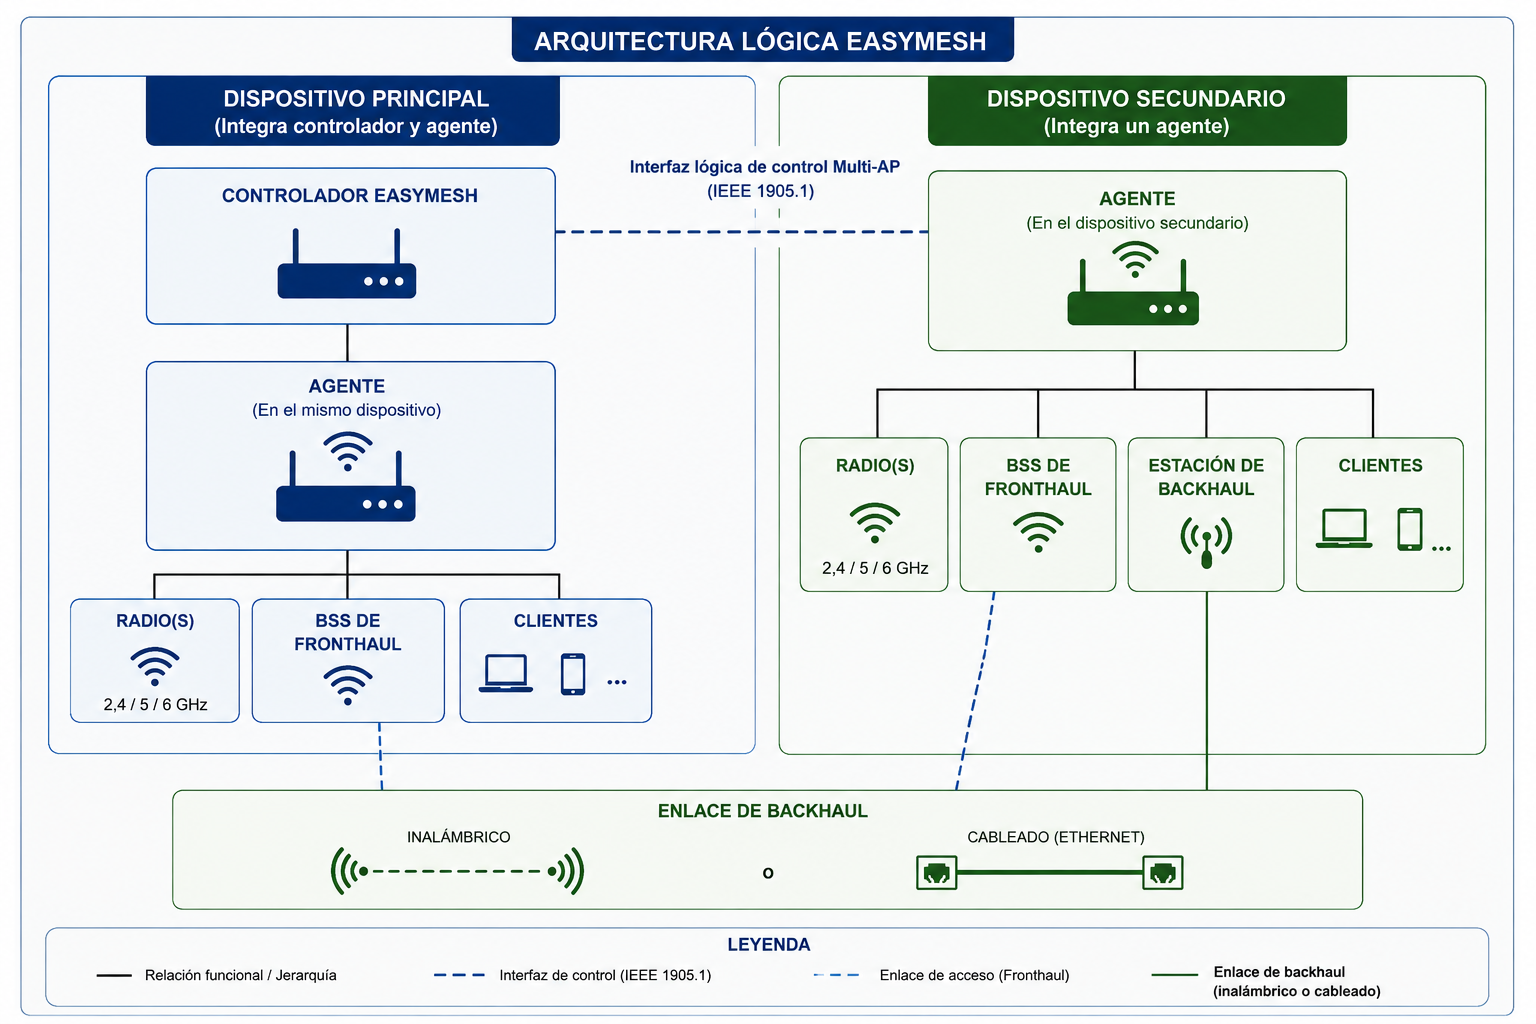
\includegraphics[width=0.92\textwidth]
    {figures/arquitectura_easymesh.png}

    \caption[Arquitectura lógica y física de una red EasyMesh.]
    {Arquitectura lógica y física de una red EasyMesh. El dispositivo
    principal integra el controlador y un agente, mientras que los
    dispositivos secundarios incorporan agentes que administran sus
    radios y puntos de acceso. Los clientes se conectan mediante enlaces
    de \textit{fronthaul} y los dispositivos Multi-AP se interconectan
    mediante enlaces de \textit{backhaul}.
    \textit{Fuente: imagen generada mediante ChatGPT (OpenAI) a partir
    de las indicaciones de la autora y basada en la especificación
    Wi-Fi EasyMesh y en IEEE~1905.1
    \cite{wifi_alliance_easymesh,ieee_1905_1}.}}

    \label{fig:arquitectura-easymesh}
\end{figure}

Desde el punto de vista de la observabilidad, la arquitectura obliga a
mantener una correspondencia entre diferentes niveles de información.
La plataforma debe relacionar el dispositivo físico, el agente, la
radio, el BSS y el cliente, además de identificar la trayectoria de
\textit{backhaul} utilizada para alcanzar el nodo principal.

Una representación incompleta de esta jerarquía puede provocar que la
plataforma detecte la presencia del cliente, pero no determine
correctamente el nodo que le proporciona servicio. Por tanto, la
\textbf{topología EasyMesh} y la
\textbf{asociación del cliente} constituyen dos elementos esenciales para
interpretar las métricas obtenidas de la red.

La arquitectura descrita proporciona el marco sobre el que actúan el
controlador y los agentes. Los apartados siguientes desarrollan por
separado las funciones de cada una de estas entidades.

\subsection{Controlador EasyMesh}
\label{subsec:controlador-easymesh}

El \textbf{controlador EasyMesh} es la entidad lógica encargada de
coordinar el funcionamiento de la red Multi-AP. Su encargada de
coordinar el funcionamiento función consiste en
mantener una visión conjunta de la infraestructura y utilizar la
información proporcionada por los agentes para aplicar las políticas de
configuración y gestión definidas para la red
\cite{wifi_alliance_easymesh}.

Dentro de una red EasyMesh existe un
\textbf{único controlador lógico}. Esta entidad puede encontrarse
integrada en el mismo dispositivo físico que uno de los agentes o
implementarse en un equipo independiente. Por tanto, el controlador no
debe interpretarse necesariamente como un dispositivo físico separado,
sino como una función específica dentro de la arquitectura.

En un despliegue residencial, el controlador se integra habitualmente en
el equipo principal conectado a la red del operador. Este dispositivo
puede desempeñar simultáneamente las funciones de
\textbf{CPE}, \textbf{\textit{gateway}}, punto de acceso,
controlador EasyMesh y agente EasyMesh. La coexistencia de estas
funciones permite concentrar la gestión de la red mallada en el equipo
principal.

El controlador mantiene información sobre la
\textbf{topología de la red}, los agentes disponibles, las interfaces de
interconexión, las radios, los puntos de acceso y los clientes asociados.
Esta información proporciona una representación lógica de los elementos
que forman la infraestructura y de las relaciones existentes entre
ellos.

La visión de la topología permite conocer qué agentes se encuentran
incorporados a la red y mediante qué enlaces alcanzan el nodo principal.
También permite distinguir entre conexiones directas y trayectorias que
atraviesan uno o varios agentes intermedios.

El controlador obtiene esta información mediante los mensajes y
procedimientos intercambiados con los agentes. La comunicación interna se
apoya en la capa de abstracción y en los mecanismos de descubrimiento
proporcionados por \textbf{IEEE~1905.1}, sobre los que EasyMesh incorpora
sus procedimientos específicos de control Multi-AP
\cite{ieee_1905_1,wifi_alliance_easymesh}.

Una de las funciones principales del controlador consiste en el
\textbf{descubrimiento y la incorporación de agentes}. Cuando un
dispositivo compatible se añade a la red, debe identificarse,
intercambiar sus capacidades y recibir la configuración necesaria para
integrarse en la infraestructura Multi-AP.

Durante este proceso, el controlador puede obtener información sobre las
interfaces disponibles, las bandas de frecuencia admitidas, los canales
soportados, las capacidades de las radios y las funciones implementadas
por el agente. Estos datos permiten adaptar la configuración a las
características reales de cada dispositivo.

El controlador también participa en la
\textbf{configuración de los puntos de acceso}. Esta configuración puede
incluir parámetros relacionados con los SSID, los mecanismos de
seguridad, las credenciales y las funciones asociadas a los BSS de
\textit{fronthaul} y \textit{backhaul}.

La aplicación de una configuración coordinada permite que varios puntos
de acceso presenten una misma red lógica a los usuarios. Aunque los BSS
compartan el mismo SSID, cada uno mantiene un BSSID propio y permanece
asociado a una radio y a un agente concretos.

Otra función relevante es la
\textbf{gestión de los recursos radioeléctricos}. El controlador puede
recopilar información sobre los canales admitidos, las preferencias de
los agentes, la utilización del medio y las condiciones observadas por
las radios. A partir de estos datos, la red puede aplicar decisiones
coordinadas de configuración.

La gestión de canales busca reducir situaciones de interferencia y
utilizar de forma más adecuada el espectro disponible. No obstante, las
acciones concretas dependen de las capacidades implementadas por los
dispositivos y de las funciones admitidas por la versión de EasyMesh
utilizada.

El controlador también puede intervenir en la
\textbf{gestión de los clientes asociados}. Para ello, recopila
información sobre las estaciones detectadas, el BSSID utilizado, la radio
correspondiente y determinadas métricas relacionadas con la calidad de
la conexión.

Esta visión permite identificar qué punto de acceso proporciona servicio
a cada cliente. Cuando un terminal cambia de asociación, el controlador
debe actualizar la relación entre la estación, el BSSID de origen y el
BSSID de destino.

La información recopilada puede utilizarse para apoyar mecanismos de
\textbf{\textit{client steering}}. Mediante estos procedimientos, el
controlador puede seleccionar un punto de acceso candidato y solicitar al
agente correspondiente que facilite o recomiende la transición del
cliente.

Sin embargo, el controlador no determina siempre de manera unilateral la
asociación final. El dispositivo cliente participa en la selección del
punto de acceso y puede aceptar, retrasar o rechazar una recomendación de
transición. Por tanto, una acción de \textit{steering} no implica
necesariamente que se produzca un cambio efectivo de asociación.

El controlador también puede utilizar la información disponible para
favorecer el \textbf{balanceo de clientes}. Este proceso busca distribuir
las estaciones y la carga entre las radios y los puntos de acceso de
acuerdo con las condiciones observadas en la red.

El balanceo no debe basarse únicamente en el número de clientes
asociados. También deben considerarse la utilización del canal, el
tráfico generado, la capacidad de cada radio, las condiciones del enlace
y las características de los terminales.

Además de las métricas relacionadas con los clientes, el controlador
recopila información sobre los
\textbf{enlaces de \textit{backhaul}}. Esta información permite conocer
la conectividad entre los nodos y evaluar la calidad de las trayectorias
utilizadas para transportar el tráfico hacia el dispositivo principal.

La calidad del \textit{backhaul} resulta especialmente importante cuando
un agente alcanza el controlador a través de otro nodo intermedio. En
este caso, el controlador debe mantener una representación de la
trayectoria completa para interpretar correctamente el rendimiento
obtenido por los clientes asociados al agente más alejado.

Desde un punto de vista funcional, el controlador participa
principalmente en el \textbf{plano de control}. Su misión consiste en
recopilar información, aplicar políticas y enviar instrucciones a los
agentes. Esto no implica necesariamente que todo el tráfico de usuario
sea procesado directamente por la entidad lógica de control.

El tráfico generado por los clientes pertenece al
\textbf{plano de datos} y atraviesa los enlaces de
\textit{fronthaul} y \textit{backhaul} correspondientes. Aunque la
función de controlador se encuentre integrada en el nodo principal, debe
diferenciarse la coordinación lógica de la red del encaminamiento de los
paquetes de usuario.

Como se representa en la
Figura~\ref{fig:arquitectura-easymesh}, el controlador mantiene una
relación lógica con todos los agentes de la infraestructura. A través de
esta relación obtiene información sobre los recursos disponibles y
coordina el funcionamiento de la red Multi-AP.

Desde el punto de vista de la observabilidad, el controlador constituye
una \textbf{fuente central de información sobre la red EasyMesh}. Su
visión debe permitir relacionar los agentes, las radios, los BSS, los
clientes y los enlaces de \textit{backhaul}.

No obstante, la información disponible para una plataforma externa
depende de que el controlador la recopile, la actualice y la exponga
mediante un modelo de datos accesible. La existencia de una métrica dentro
de la arquitectura interna de EasyMesh no garantiza que dicha métrica se
encuentre disponible mediante TR-181 o pueda consultarse desde el ACS.

En el laboratorio desarrollado, el
\textbf{controlador EasyMesh se encuentra integrado en el CPE TP-Link
HX141}. Este equipo constituye el nodo principal de la red mallada y el
único dispositivo registrado directamente en GenieACS mediante
TR-069/CWMP.

Los dos dispositivos TP-Link HX141 restantes actúan como agentes y no se
registran en el ACS como CPE independientes. En consecuencia, la
información relacionada con estos nodos debe ser recopilada por el
controlador y expuesta a través del modelo de datos del CPE.

Esta organización convierte al controlador en el
\textbf{punto principal de observación de la red interna}. La plataforma
de monitorización depende de la información expuesta por este elemento
para identificar la topología, localizar al cliente móvil y mantener la
trazabilidad de sus cambios de asociación.

Si el controlador no actualiza correctamente la información de un agente
o de un cliente, la conectividad puede continuar funcionando mientras la
plataforma conserva una representación incompleta o desactualizada. Esta
situación origina el punto ciego de visibilidad analizado en el presente
trabajo.

Por tanto, las funciones del controlador resultan relevantes tanto para
la coordinación de la red como para su monitorización. El controlador
debe mantener una representación coherente de la infraestructura y
proporcionar información suficiente para conocer
\textbf{qué agentes forman la red}, \textbf{cómo se encuentran
interconectados} y \textbf{qué nodo proporciona servicio a cada cliente}.

\subsection{Agentes EasyMesh}
\label{subsec:agentes-easymesh}

Los \textbf{agentes EasyMesh} son las entidades lógicas encargadas de
administrar los recursos de red disponibles en los dispositivos
Multi-AP. Cada agente mantiene información sobre sus interfaces, radios,
puntos de acceso, clientes asociados y enlaces de
\textit{backhaul}, y ejecuta las acciones de configuración y control
solicitadas por el controlador \cite{wifi_alliance_easymesh}.

Un agente puede encontrarse integrado en el mismo dispositivo físico que
el controlador o implementarse en un nodo secundario de la red. En un
despliegue residencial, el equipo principal suele incorporar
simultáneamente las funciones de controlador y agente, mientras que los
dispositivos distribuidos por la vivienda implementan normalmente la
función de agente.

La existencia de un agente en el dispositivo principal resulta necesaria
porque dicho equipo también puede disponer de radios, puntos de acceso y
clientes asociados. Por tanto, aunque el controlador coordine la red,
los recursos inalámbricos locales del dispositivo principal se
administran mediante su correspondiente entidad agente.

Cada agente puede gestionar una o varias \textbf{radios Wi-Fi}. Estas
radios pueden operar en distintas bandas de frecuencia y utilizar
diferentes canales, anchos de canal, niveles de potencia y capacidades
físicas. El agente mantiene información sobre estos recursos y la pone a
disposición del controlador mediante los procedimientos definidos por la
arquitectura EasyMesh.

Las radios representan las interfaces físicas sobre las que se configuran
los diferentes \textbf{BSS}. Un agente puede administrar varios BSS,
cada uno identificado mediante un BSSID propio. Algunos de ellos se
utilizan para proporcionar conectividad a los clientes, mientras que
otros pueden participar en el establecimiento de enlaces inalámbricos de
\textit{backhaul}.

Los BSS destinados a atender terminales convencionales se denominan
\textbf{BSS de \textit{fronthaul}}. Los teléfonos móviles, ordenadores,
tabletas y demás estaciones Wi-Fi se asocian a estos puntos de acceso para
acceder a la red local y a los servicios externos.

El agente mantiene la relación entre cada cliente y el BSS al que se
encuentra asociado. Esta relación permite conocer la dirección MAC de la
estación, el BSSID utilizado, la radio correspondiente y el dispositivo
Multi-AP que proporciona la conectividad.

Cuando el agente participa en un \textit{backhaul} inalámbrico, también
puede incorporar una \textbf{estación de \textit{backhaul}}. Esta
interfaz actúa como cliente de otro punto de acceso EasyMesh para
establecer la comunicación con un nodo situado en un nivel superior de la
topología.

Por tanto, un dispositivo secundario puede desempeñar simultáneamente dos
funciones dentro del plano de datos. Por una parte, actúa como estación
respecto al nodo que le proporciona el enlace de
\textit{backhaul}. Por otra, funciona como punto de acceso para los
clientes conectados mediante el \textit{fronthaul}.

Esta doble función puede representarse mediante la siguiente secuencia:

\[
    \text{Cliente}
    \xrightarrow{\text{\textit{fronthaul}}}
    \text{Agente secundario}
    \xrightarrow{\text{\textit{backhaul}}}
    \text{Nodo superior}.
\]

Cuando el agente utiliza otro agente intermedio para alcanzar el
dispositivo principal, la comunicación atraviesa varios enlaces de
\textit{backhaul}. En este caso, cada nodo participa en el transporte del
tráfico y forma parte de la trayectoria utilizada por los clientes
situados en niveles inferiores de la topología.

Los agentes proporcionan al controlador información sobre sus
\textbf{capacidades}. Esta información puede incluir las bandas de
frecuencia admitidas, los canales soportados, el número de radios, los
tipos de BSS disponibles y las funciones de gestión implementadas por el
dispositivo \cite{wifi_alliance_easymesh}.

El conocimiento de estas capacidades permite que el controlador adapte
las decisiones de configuración a los recursos reales de cada agente.
Dos dispositivos pertenecientes a la misma red pueden disponer de
diferentes generaciones de Wi-Fi, bandas de frecuencia, anchos de canal o
funciones opcionales.

Los agentes también informan sobre la
\textbf{configuración y el estado de sus radios}. Entre los datos
relevantes se encuentran el canal utilizado, el ancho de canal, el estado
operativo, los BSS configurados y las estaciones asociadas.

La disponibilidad concreta de estas métricas depende de la versión de la
especificación implementada y de las capacidades proporcionadas por el
fabricante. La existencia de una función dentro de EasyMesh no implica
necesariamente que toda su información se exponga posteriormente mediante
el modelo de datos TR-181.

Otra función de los agentes consiste en ejecutar las
\textbf{acciones de configuración} solicitadas por el controlador. Estas
acciones pueden afectar a los puntos de acceso, los canales, la potencia,
los parámetros de seguridad o determinadas funciones de gestión de
clientes.

El agente recibe la solicitud, aplica la operación cuando dispone de las
capacidades necesarias y comunica el resultado al controlador. Esta
separación permite que las decisiones se adopten desde una visión global,
mientras que su ejecución se realiza sobre los recursos locales de cada
dispositivo.

Los agentes participan además en el
\textbf{descubrimiento de la topología}. Mediante la comunicación con los
dispositivos vecinos, permiten identificar las interfaces y los enlaces
que forman la red. Esta información se transmite al controlador para
construir una representación conjunta de la infraestructura.

La comunicación interna utiliza mensajes transportados mediante los
mecanismos definidos por IEEE~1905.1. Esta capa permite identificar
dispositivos e interfaces y facilita el intercambio de información de
control entre elementos conectados mediante tecnologías diferentes
\cite{ieee_1905_1}.

Los agentes también recopilan información sobre los
\textbf{clientes asociados}. Esta información resulta necesaria para
determinar qué terminal recibe servicio desde cada punto de acceso y para
observar los cambios producidos durante los desplazamientos dentro de la
vivienda.

Entre los datos relacionados con una estación pueden encontrarse su
dirección MAC, el BSSID utilizado, el estado de asociación, el tráfico
transmitido y recibido y determinadas métricas de calidad radio. La
disponibilidad, semántica y frecuencia de actualización de estos valores
dependen de la implementación del dispositivo.

El agente puede participar en procedimientos de
\textbf{\textit{client steering}} cuando recibe una instrucción del
controlador. En este caso, utiliza los mecanismos disponibles para
recomendar o favorecer que el cliente abandone el punto de acceso actual
y se asocie a otro BSS candidato.

Sin embargo, el agente no controla de forma absoluta la decisión final
del terminal. El cliente puede aceptar o rechazar la transición según sus
propios algoritmos, capacidades y condiciones de conexión. Por tanto, la
ejecución de una acción de \textit{steering} debe diferenciarse del
cambio efectivo de asociación.

Los agentes también pueden recopilar
\textbf{métricas de los enlaces de \textit{backhaul}}. Estas métricas
permiten evaluar la comunicación entre los nodos y detectar si el enlace
utilizado por un agente puede limitar el rendimiento obtenido por sus
clientes.

La calidad del enlace de \textit{backhaul} debe analizarse junto con la
calidad del \textit{fronthaul}. Un cliente puede presentar un nivel de
señal adecuado respecto al agente y, al mismo tiempo, experimentar una
degradación debido a una conexión deficiente entre dicho agente y el nodo
superior.

Desde el punto de vista del plano de control, el agente actúa como
\textbf{intermediario entre los recursos locales y el controlador}. El
agente convierte el estado de sus radios, puntos de acceso, interfaces y
clientes en información que puede utilizarse para mantener y administrar
la red Multi-AP.

Desde el punto de vista del plano de datos, el dispositivo que incorpora
el agente proporciona conectividad a los clientes y transporta su tráfico
a través de la infraestructura. Deben diferenciarse ambas funciones, ya
que la entidad lógica agente participa en la gestión, mientras que las
interfaces físicas transportan las tramas de usuario.

Como se representa en la
Figura~\ref{fig:arquitectura-easymesh}, cada agente administra sus radios
y puntos de acceso, mientras que el controlador mantiene la coordinación
global. Esta relación permite distribuir las funciones de acceso por la
vivienda sin administrar cada nodo como una red independiente.

Desde el punto de vista de la observabilidad, cada agente constituye una
\textbf{fuente local de información}. Sin embargo, en la arquitectura
utilizada en este proyecto, la plataforma de gestión no consulta
directamente a los agentes mediante TR-069, sino que obtiene su
información a través del controlador integrado en el CPE.

En el laboratorio desarrollado, los dos dispositivos TP-Link HX141
secundarios desempeñan la función de
\textbf{agentes EasyMesh}. Cada uno amplía la cobertura inalámbrica y
puede proporcionar conectividad al terminal móvil utilizado durante las
pruebas.

Estos agentes no se registran en GenieACS como CPE independientes. Por
tanto, los datos relativos a sus radios, puntos de acceso, enlaces de
\textit{backhaul} y clientes asociados deben recopilarse por medio del
controlador y exponerse dentro del modelo de datos del dispositivo
principal.

Esta situación condiciona la monitorización. Si la información de un
agente no se incorpora correctamente al árbol de parámetros del CPE, la
plataforma puede detectar la presencia general del cliente, pero no
identificar con precisión el nodo que le proporciona servicio.

Por ello, la monitorización de los agentes requiere mantener una
correspondencia entre:

\begin{itemize}
    \item el \textbf{dispositivo físico};
    \item el \textbf{agente EasyMesh};
    \item las \textbf{radios administradas};
    \item los \textbf{BSS configurados};
    \item los \textbf{clientes asociados};
    \item los \textbf{enlaces de \textit{backhaul}}.
\end{itemize}

La conservación de esta jerarquía permite interpretar correctamente las
métricas y mantener la trazabilidad del terminal cuando cambia desde el
controlador hacia un agente o entre diferentes agentes de la red.

En consecuencia, los agentes no actúan únicamente como extensores de
cobertura. Constituyen entidades administradas que
\textbf{ejecutan configuraciones}, \textbf{recopilan telemetría},
\textbf{atienden a los clientes} y
\textbf{mantienen los enlaces necesarios para integrarse en la
topología EasyMesh}.

\subsection{Métricas relevantes en una red EasyMesh}
\label{subsec:metricas-relevantes-red-easymesh}

La monitorización de una red EasyMesh requiere recopilar información
procedente de diferentes niveles de la arquitectura. No basta con conocer
el estado general del CPE o la presencia de un cliente en la red, sino que
resulta necesario relacionar el \textbf{dispositivo físico}, el
\textbf{agente EasyMesh}, la \textbf{radio}, el
\textbf{BSS}, el \textbf{cliente asociado} y los enlaces utilizados para
transportar su tráfico.

La especificación EasyMesh contempla el intercambio de información sobre
la topología, las capacidades de los dispositivos, las radios, los
puntos de acceso, los clientes y los enlaces de la red Multi-AP
\cite{wifi_alliance_easymesh}. Parte de esta información puede
representarse posteriormente mediante el modelo de datos TR-181,
especialmente a través de la estructura
\texttt{Device.WiFi.DataElements}
\cite{bbf_tr181}.

Las métricas relevantes pueden organizarse en diferentes grupos según el
elemento de la red que describen y la finalidad con la que se utilizan.

\subsubsection*{Métricas de topología y dispositivos}

Las \textbf{métricas de topología} permiten identificar los equipos que
forman la red EasyMesh y las relaciones existentes entre ellos. Este
grupo incluye la identidad de los dispositivos, su estado operativo, el
tipo de entidad implementada y los enlaces empleados para conectarse con
el resto de la infraestructura.

Entre la información relevante se encuentran:

\begin{itemize}
    \item el identificador del dispositivo Multi-AP;
    \item el fabricante, el modelo y la versión de software;
    \item el estado activo o inactivo del dispositivo;
    \item la función desempeñada dentro de la red;
    \item el nodo superior mediante el que alcanza el
    \textit{gateway};
    \item el tipo de enlace utilizado para el \textit{backhaul};
    \item el número de saltos existente hasta el nodo principal.
\end{itemize}

Estas métricas permiten reconstruir la
\textbf{topología lógica de la red} y diferenciar entre conexiones
directas y trayectorias que atraviesan agentes intermedios. Esta
información resulta necesaria para interpretar el rendimiento de los
clientes conectados a nodos secundarios.

La identidad de cada nodo debe mantenerse mediante un
\textbf{identificador estable}. Las posiciones ocupadas por los
dispositivos dentro de una tabla o de un árbol de parámetros pueden
cambiar después de un reinicio o de una actualización de la topología.
Por tanto, no deben utilizarse por sí solas como identificadores
permanentes.

\subsubsection*{Métricas de radio}

Las \textbf{métricas de radio} describen las interfaces inalámbricas
administradas por cada agente. Estas métricas permiten conocer las
condiciones bajo las que operan los puntos de acceso y detectar posibles
limitaciones relacionadas con la configuración o con el entorno
radioeléctrico.

Entre los principales parámetros se encuentran:

\begin{itemize}
    \item la banda de frecuencia utilizada;
    \item el canal de operación;
    \item el ancho de canal;
    \item la potencia de transmisión;
    \item el estado operativo de la radio;
    \item el nivel de ruido;
    \item la utilización u ocupación del canal;
    \item las capacidades y estándares Wi-Fi admitidos.
\end{itemize}

La \textbf{banda de frecuencia}, el \textbf{canal} y el
\textbf{ancho de canal} permiten caracterizar la configuración de la
radio. El nivel de ruido y la utilización del canal aportan información
sobre las condiciones del medio, aunque su disponibilidad y significado
exacto dependen de la implementación realizada por el fabricante.

Estas métricas deben interpretarse conjuntamente. Una radio puede utilizar
un ancho de canal elevado y admitir tasas físicas altas, pero ofrecer un
rendimiento reducido si el canal presenta una ocupación intensa o unas
condiciones de interferencia desfavorables.

\subsubsection*{Métricas de BSS y puntos de acceso}

Cada radio puede alojar uno o varios BSS. Las
\textbf{métricas de BSS} permiten identificar los puntos de acceso
configurados y relacionarlos con las radios y los agentes que los
administran.

Entre la información relevante se encuentra:

\begin{itemize}
    \item el \textbf{SSID} anunciado;
    \item el \textbf{BSSID} del punto de acceso;
    \item el estado habilitado o deshabilitado;
    \item la radio sobre la que se encuentra configurado;
    \item su función de \textit{fronthaul} o
    \textit{backhaul};
    \item el número de clientes asociados;
    \item el instante del último cambio de estado.
\end{itemize}

El SSID identifica la red lógica presentada al usuario, mientras que el
BSSID permite determinar el punto de acceso concreto que proporciona
servicio. En una red EasyMesh, varios BSS pueden anunciar el mismo SSID,
por lo que la identificación del BSSID resulta imprescindible para
localizar correctamente al cliente.

La relación entre \textbf{BSSID, radio, agente y dispositivo físico}
constituye una de las asociaciones fundamentales para la monitorización.
Sin esta correspondencia, la plataforma puede detectar al terminal, pero
no determinar con precisión el nodo desde el que recibe conectividad.

\subsubsection*{Métricas de clientes asociados}

Las \textbf{métricas de cliente} describen las estaciones Wi-Fi
asociadas a los diferentes puntos de acceso. Su finalidad consiste en
identificar los terminales, conocer el estado de su enlace y mantener la
trazabilidad cuando cambian entre distintos nodos.

Entre las métricas más relevantes se encuentran:

\begin{itemize}
    \item la dirección MAC del cliente;
    \item el BSSID al que se encuentra asociado;
    \item el instante de asociación o última conexión;
    \item el nivel de señal recibido;
    \item la última tasa de transmisión en sentido ascendente;
    \item la última tasa de transmisión en sentido descendente;
    \item los bytes y paquetes transmitidos y recibidos;
    \item los errores de transmisión y recepción;
    \item el número de retransmisiones.
\end{itemize}

La \textbf{dirección MAC} se utiliza como identificador principal del
cliente, ya que permite relacionar su presencia en diferentes ramas,
radios y puntos de acceso. La dirección IP y el nombre del dispositivo
pueden utilizarse como atributos auxiliares, pero no siempre permanecen
constantes ni se encuentran disponibles.

El \textbf{nivel de señal} permite aproximar la calidad radioeléctrica
del enlace entre el cliente y el punto de acceso. Sin embargo, no debe
interpretarse de forma aislada, ya que una señal elevada no garantiza un
caudal útil alto cuando existen interferencias, congestión,
retransmisiones o limitaciones en el enlace de
\textit{backhaul}.

Las tasas de transmisión ascendente y descendente representan las
condiciones físicas recientes del enlace. Estas tasas no equivalen al
caudal obtenido por una aplicación, porque no descuentan el tráfico de
control, los tiempos de acceso al medio, las cabeceras ni las
retransmisiones.

Los contadores de bytes, paquetes, errores y retransmisiones permiten
analizar la actividad y la estabilidad de la conexión. Para convertir
estos contadores acumulados en indicadores temporales resulta necesario
calcular su variación entre observaciones sucesivas.

\subsubsection*{Métricas de \textit{backhaul}}

Las \textbf{métricas de \textit{backhaul}} permiten caracterizar los
enlaces utilizados para interconectar los nodos EasyMesh. Estas métricas
resultan especialmente relevantes cuando un cliente se encuentra
asociado a un agente secundario, ya que su tráfico debe atravesar uno o
varios enlaces antes de alcanzar el nodo principal.

Entre la información de interés se encuentra:

\begin{itemize}
    \item el tipo de enlace, cableado o inalámbrico;
    \item los dispositivos situados en cada extremo;
    \item la interfaz utilizada;
    \item la banda, el canal y el ancho de canal;
    \item la tasa física del enlace;
    \item el nivel de señal o la calidad del enlace;
    \item el estado operativo;
    \item el número de saltos hasta el nodo principal.
\end{itemize}

La calidad del \textit{backhaul} debe analizarse conjuntamente con la del
\textit{fronthaul}. Un cliente puede mantener una buena conexión con el
agente y experimentar una degradación debido a una capacidad insuficiente
o a unas condiciones radioeléctricas desfavorables entre dicho agente y
el nodo superior.

En una topología en cascada, la interpretación debe considerar la
\textbf{trayectoria completa}. La degradación de cualquiera de los
enlaces intermedios puede afectar a todos los clientes cuyo tráfico
atraviesa dicho segmento.

\subsubsection*{Métricas de movilidad y \textit{steering}}

Las \textbf{métricas de movilidad} permiten observar los cambios de
asociación realizados por los clientes. Estas métricas deben diferenciar
entre las acciones solicitadas por la infraestructura y las transiciones
que finalmente completa el terminal.

La información relevante puede incluir:

\begin{itemize}
    \item el cliente afectado;
    \item el BSSID de origen;
    \item el BSSID de destino;
    \item el instante de la solicitud;
    \item el resultado de la operación;
    \item la causa de la transición;
    \item el tiempo transcurrido hasta observar la nueva asociación;
    \item el número de intentos de \textit{steering}.
\end{itemize}

Una solicitud de \textit{steering} no representa necesariamente un
cambio efectivo de asociación. Por este motivo, la plataforma debe
comprobar si el cliente desaparece del BSS de origen y aparece
posteriormente en el BSS de destino.

La correlación temporal entre ambas observaciones permite reconstruir el
desplazamiento del terminal. No obstante, el intervalo observado incluye
los retardos de actualización y adquisición de la telemetría, por lo que
no debe interpretarse automáticamente como la duración exacta del proceso
radio.

\subsubsection*{Antigüedad y validez de la telemetría}

Toda métrica debe estar acompañada de información temporal que permita
determinar su \textbf{antigüedad}. Un valor puede ser técnicamente
correcto en el momento de su adquisición y dejar de representar el estado
actual después de un cambio de asociación, un reinicio o una
reconfiguración de la red.

Entre los elementos temporales relevantes se encuentran:

\begin{itemize}
    \item el instante de recopilación;
    \item el instante de la última actualización;
    \item el intervalo de adquisición;
    \item el tiempo transcurrido desde el último cambio;
    \item la edad del dato en el momento de su representación.
\end{itemize}

La antigüedad debe considerarse una parte inseparable de la métrica. Por
ejemplo, una asociación observada varios minutos antes no debe utilizarse
sin comprobar si continúa vigente. Esta consideración resulta
especialmente importante durante las pruebas de movilidad y
\textit{roaming}.

\subsubsection*{Métricas directas e indicadores derivados}

Las métricas recopiladas directamente de los dispositivos no siempre
proporcionan por sí solas la información necesaria para el diagnóstico.
Por esta razón, debe diferenciarse entre
\textbf{métricas directas} e \textbf{indicadores derivados}.

Las métricas directas corresponden a valores expuestos por el equipo,
como el nivel de señal, la tasa física, los bytes transmitidos o el
BSSID de asociación. Los indicadores derivados se obtienen mediante
operaciones aplicadas sobre una o varias métricas.

Entre los posibles indicadores derivados se encuentran:

\begin{itemize}
    \item la tasa de transferencia calculada a partir de contadores;
    \item la tasa de errores o retransmisiones;
    \item el tiempo de permanencia en cada nodo;
    \item el número de cambios de asociación;
    \item la antigüedad de la telemetría;
    \item la duración observada de una transición;
    \item la disponibilidad del cliente durante un intervalo;
    \item la identificación del nodo que proporciona servicio.
\end{itemize}

La obtención de estos indicadores requiere mantener una
\textbf{correlación temporal} entre las observaciones. También requiere
normalizar los identificadores para evitar que los cambios de posición
dentro del modelo de datos fragmenten las series correspondientes a un
mismo cliente.

La estructura \texttt{Device.WiFi.DataElements} de TR-181 permite
representar una red Wi-Fi formada por uno o varios dispositivos, junto
con sus radios, BSS y estaciones asociadas
\cite{bbf_tr181}. No obstante, la disponibilidad real de cada parámetro
depende de la versión del modelo de datos, del firmware y de la
implementación realizada por el fabricante.

Por tanto, el catálogo de métricas utilizado en una plataforma de
monitorización debe distinguir entre:

\begin{itemize}
    \item parámetros definidos por la especificación;
    \item parámetros realmente expuestos por el dispositivo;
    \item valores actualizados de manera fiable;
    \item métricas cuya unidad o semántica se encuentra documentada;
    \item indicadores que deben calcularse mediante procesamiento
    adicional.
\end{itemize}

En el presente proyecto, esta clasificación permite seleccionar las
métricas utilizadas para observar la
\textbf{topología EasyMesh}, la
\textbf{asociación del cliente}, la
\textbf{calidad del enlace radio}, la
\textbf{actividad de tráfico}, la
\textbf{movilidad entre nodos} y la
\textbf{antigüedad de la telemetría}.

El análisis detallado de la representación de estos elementos en
TR-181 se desarrolla en la Sección~\ref{sec:tr-181}. Posteriormente, el
catálogo definitivo establece para cada métrica su ruta, unidad,
procedimiento de adquisición, periodicidad, tratamiento y principales
limitaciones.

\section{IEEE 1905.1}
\label{sec:ieee-1905-1}

Las redes domésticas pueden combinar diferentes tecnologías de
comunicación, como Ethernet, Wi-Fi, redes sobre líneas eléctricas o
enlaces sobre cable coaxial. Cada tecnología utiliza sus propios
mecanismos de identificación, configuración y transporte, lo que
dificulta la construcción de una visión común de los dispositivos y de
los enlaces que forman la infraestructura.

El estándar \textbf{IEEE~1905.1} define una
\textbf{capa de abstracción para redes domésticas heterogéneas}. Su
finalidad consiste en proporcionar una interfaz común que permita
representar y coordinar diferentes tecnologías de comunicación sin
modificar el funcionamiento interno de cada una de ellas
\cite{ieee_1905_1}.

La capa de abstracción de IEEE~1905.1 se sitúa funcionalmente entre la
\textbf{capa de enlace} y la \textbf{capa de red}. Desde esta posición,
permite ocultar parte de las particularidades de las interfaces físicas y
presentar una representación conjunta de los dispositivos, las
interfaces y los enlaces disponibles en la red.

Entre las tecnologías consideradas por el estándar se encuentran
\textbf{IEEE~802.11}, utilizada por las redes Wi-Fi;
\textbf{Ethernet}, empleada en las conexiones cableadas;
\textbf{IEEE~1901}, destinada a comunicaciones sobre líneas eléctricas;
y \textbf{MoCA}, utilizada para transmitir información mediante cable
coaxial \cite{ieee_1905_1}.

IEEE~1905.1 no sustituye a estas tecnologías ni modifica sus
procedimientos MAC o PHY. Cada interfaz continúa operando conforme a su
propio estándar, mientras que la capa de abstracción proporciona
mecanismos comunes para identificarlas, descubrirlas y utilizarlas de
forma coordinada.

Un dispositivo compatible con IEEE~1905.1 puede disponer de varias
interfaces pertenecientes a tecnologías diferentes. Para representar el
equipo de manera unificada, el estándar utiliza un
\textbf{identificador lógico del dispositivo}, independiente de las
direcciones específicas asociadas a cada interfaz física.

Esta separación permite diferenciar entre:

\begin{itemize}
    \item el \textbf{dispositivo IEEE~1905.1};
    \item las \textbf{interfaces de red} disponibles en dicho
    dispositivo;
    \item las \textbf{tecnologías de enlace} utilizadas;
    \item los \textbf{dispositivos vecinos};
    \item los \textbf{enlaces} establecidos entre las interfaces.
\end{itemize}

La identificación conjunta de estos elementos permite construir una
\textbf{representación lógica de la topología}. Esta representación
describe qué dispositivos forman la red, qué interfaces pertenecen a
cada equipo y mediante qué enlaces se encuentran interconectados.

El estándar define mecanismos relacionados con el
\textbf{descubrimiento de dispositivos}, la
\textbf{obtención de información de topología}, la
\textbf{selección de trayectorias}, la
\textbf{autoconfiguración} y el intercambio de información asociada a la
calidad de los enlaces \cite{ieee_1905_1}.

La comunicación entre los dispositivos se realiza mediante
\textbf{mensajes de control IEEE~1905.1}. Estos mensajes permiten
solicitar, comunicar o actualizar información relacionada con el estado
de la red. La estructura de los mensajes facilita la incorporación de
diferentes tipos de información sin depender directamente del medio
físico utilizado para transportarlos.

Los mensajes de control se encapsulan en
\textbf{tramas CMDU}
(\textit{Control Message Data Unit}). Cada CMDU identifica el tipo de
operación realizada y puede contener uno o varios elementos de
información. Estos elementos se organizan mediante estructuras
\textbf{TLV} (\textit{Type-Length-Value}), que permiten indicar el tipo,
la longitud y el contenido de cada dato intercambiado.

Esta organización proporciona un formato extensible para transportar
información sobre dispositivos, interfaces, vecinos, enlaces y otras
características de la red. Las extensiones posteriores pueden incorporar
nuevos tipos de mensajes o TLV sin sustituir los mecanismos básicos
proporcionados por la capa IEEE~1905.1.

La arquitectura \textbf{Wi-Fi EasyMesh} utiliza IEEE~1905.1 como base
para la comunicación interna entre el controlador y los agentes. Sobre
los mecanismos generales del estándar, EasyMesh define mensajes,
procedimientos y objetos específicos para administrar una
\textbf{infraestructura Multi-AP}
\cite{wifi_alliance_easymesh,ieee_1905_1}.

De este modo, IEEE~1905.1 proporciona la capacidad de identificar los
dispositivos y representar sus interfaces y enlaces, mientras que
EasyMesh incorpora la lógica necesaria para coordinar radios, puntos de
acceso, clientes y enlaces de \textit{backhaul} dentro de una red Wi-Fi
mallada.

La relación entre ambos elementos puede resumirse de la siguiente forma:

\[
    \text{IEEE~1905.1}
    \longrightarrow
    \text{descubrimiento, abstracción y comunicación}
\]

\[
    \text{EasyMesh}
    \longrightarrow
    \text{coordinación y gestión de la red Multi-AP}
\]

La comunicación IEEE~1905.1 se produce
\textbf{dentro de la red doméstica}. Los mensajes se intercambian entre
los dispositivos que forman la infraestructura y no constituyen, por sí
mismos, un mecanismo de gestión remota entre el domicilio y la plataforma
del operador.

Esta diferencia resulta esencial para el presente proyecto. IEEE~1905.1
permite la coordinación interna entre el controlador y los agentes,
mientras que \textbf{TR-069/CWMP} se utiliza para la comunicación remota
entre el CPE y el ACS. Por otra parte, \textbf{TR-181} proporciona el
modelo de datos empleado para representar y exponer la información del
dispositivo.

Por tanto, cada tecnología desempeña una función diferente:

\begin{itemize}
    \item \textbf{IEEE~1905.1} permite descubrir los dispositivos,
    representar la topología e intercambiar información dentro de la red
    doméstica.

    \item \textbf{EasyMesh} define la organización y la coordinación de
    los elementos que forman la red Multi-AP.

    \item \textbf{TR-181} estructura los parámetros de configuración,
    estado y telemetría que expone el CPE.

    \item \textbf{TR-069/CWMP} permite consultar y gestionar remotamente
    dichos parámetros desde un ACS.
\end{itemize}

Desde el punto de vista de la observabilidad, IEEE~1905.1 constituye una
\textbf{fuente interna de información sobre la topología EasyMesh}. Sin
embargo, la plataforma de gestión no accede directamente a los mensajes
intercambiados entre el controlador y los agentes. Para que esta
información sea observable desde el exterior, el CPE debe recopilarla y
representarla mediante parámetros accesibles a través de su modelo de
datos.

En el laboratorio desarrollado, los dispositivos TP-Link HX141 utilizan
los mecanismos internos de la red EasyMesh para mantener la comunicación
entre el controlador y los agentes. La plataforma de monitorización
consulta posteriormente la información que el controlador expone
mediante TR-181 y TR-069/CWMP.

En consecuencia, IEEE~1905.1 forma parte del
\textbf{plano interno de coordinación de la red}, mientras que TR-181 y
TR-069/CWMP forman parte de la cadena utilizada para proporcionar
visibilidad a la plataforma externa. La correspondencia entre ambos
ámbitos determina qué información de la red mallada puede observarse,
con qué nivel de detalle y con qué frecuencia de actualización.

Los apartados siguientes desarrollan la
\textbf{función de IEEE~1905.1 dentro de EasyMesh}, la
\textbf{comunicación interna entre el controlador y los agentes}, la
\textbf{información intercambiada en la red Mesh} y las diferencias
existentes entre \textbf{IEEE~1905.1}, \textbf{TR-069} y
\textbf{TR-181}.

\subsection{Función de IEEE 1905.1 en EasyMesh}
\label{subsec:funcion-ieee-1905-1-easymesh}

La arquitectura \textbf{Wi-Fi EasyMesh} utiliza IEEE~1905.1 como base
para establecer la comunicación de control entre los dispositivos que
forman la red Multi-AP. Esta relación permite separar las funciones
generales de descubrimiento y representación de la red de los
procedimientos específicos utilizados para coordinar el controlador y
los agentes EasyMesh
\cite{ieee_1905_1,wifi_alliance_easymesh}.

IEEE~1905.1 proporciona una \textbf{capa de abstracción común} sobre las
diferentes tecnologías de enlace presentes en una red doméstica. Esta
capa permite identificar dispositivos, interfaces y enlaces sin depender
exclusivamente de las características particulares de Ethernet, Wi-Fi,
redes sobre líneas eléctricas o conexiones sobre cable coaxial
\cite{ieee_1905_1}.

La capa de abstracción no sustituye a las tecnologías subyacentes. Las
interfaces Ethernet continúan funcionando conforme a IEEE~802.3 y las
interfaces Wi-Fi mantienen los procedimientos MAC y PHY definidos por
IEEE~802.11. IEEE~1905.1 añade los mecanismos necesarios para
\textbf{representar estas interfaces dentro de una visión común de la
red}.

Esta capacidad resulta especialmente útil en EasyMesh, ya que los
dispositivos pueden interconectarse mediante enlaces de
\textit{backhaul} cableados o inalámbricos. El controlador debe mantener
una representación coherente de la topología con independencia del medio
físico empleado por cada enlace.

Por tanto, IEEE~1905.1 permite que la arquitectura EasyMesh trate los
diferentes enlaces como componentes de una misma infraestructura lógica.
Un agente conectado mediante Ethernet y otro conectado mediante Wi-Fi
pueden formar parte de la misma red Multi-AP y comunicarse con el
controlador a través de una interfaz de control común.

Una de las funciones principales de IEEE~1905.1 dentro de EasyMesh es el
\textbf{descubrimiento de los dispositivos}. Los nodos intercambian
información que permite identificar los equipos compatibles presentes en
la red y determinar las interfaces mediante las que se encuentran
conectados.

El descubrimiento constituye el primer paso para construir la
\textbf{topología de la red}. A partir de la información recibida, puede
determinarse qué dispositivos forman la infraestructura, qué interfaces
pertenecen a cada equipo y qué enlaces existen entre los diferentes
nodos.

Esta representación permite diferenciar entre un agente conectado
directamente al dispositivo principal y otro que utiliza un agente
intermedio para alcanzar el controlador. De este modo, pueden
representarse tanto topologías próximas a una estrella como
configuraciones en cascada con varios saltos de
\textit{backhaul}.

IEEE~1905.1 también proporciona el mecanismo utilizado para transportar
\textbf{mensajes de control} entre los elementos de la red. EasyMesh
utiliza esta capacidad para intercambiar la información y las órdenes
necesarias para gestionar la infraestructura Multi-AP
\cite{wifi_alliance_easymesh,ieee_1905_1}.

Sobre esta base, EasyMesh incorpora procedimientos específicos
relacionados con:

\begin{itemize}
    \item la incorporación y configuración de agentes;
    \item la consulta de las capacidades de los dispositivos;
    \item la configuración de radios y puntos de acceso;
    \item la obtención de información sobre la topología;
    \item la recopilación de métricas de radios, BSS y clientes;
    \item la supervisión de los enlaces de \textit{backhaul};
    \item la gestión de canales y recursos radioeléctricos;
    \item las operaciones de \textit{client steering}.
\end{itemize}

Por consiguiente, debe diferenciarse entre la
\textbf{infraestructura de comunicación proporcionada por IEEE~1905.1}
y la \textbf{lógica de gestión definida por EasyMesh}. IEEE~1905.1
proporciona los mecanismos comunes de identificación, descubrimiento,
representación e intercambio de mensajes, mientras que EasyMesh
especifica cómo se utilizan dichos mecanismos para administrar una red
Wi-Fi Multi-AP.

Esta relación puede representarse de forma simplificada mediante la
siguiente secuencia:

\[
    \text{Tecnologías de enlace}
    \longrightarrow
    \text{IEEE~1905.1}
    \longrightarrow
    \text{EasyMesh}
\]

En esta secuencia, las tecnologías de enlace proporcionan la conectividad
física y de nivel de enlace. IEEE~1905.1 ofrece una capa común para
representarlas y comunicarlas, mientras que EasyMesh incorpora las
funciones de coordinación necesarias para gestionar los puntos de acceso,
los agentes y los clientes.

Otra función relevante de IEEE~1905.1 consiste en permitir que la
comunicación de control sea relativamente independiente de la trayectoria
seguida por el tráfico. Los mensajes pueden transportarse a través de las
interfaces disponibles en la red, siempre que exista conectividad entre
los dispositivos participantes.

Esta independencia facilita que el controlador mantenga comunicación con
los agentes aunque la topología utilice diferentes tecnologías o cambie
la trayectoria de \textit{backhaul}. No obstante, la pérdida completa de
conectividad con un agente impide que el controlador reciba información
actualizada o envíe nuevas instrucciones.

La información intercambiada mediante IEEE~1905.1 pertenece al
\textbf{plano interno de control de la red doméstica}. Este plano debe
diferenciarse del tráfico de usuario, que circula a través de los enlaces
de \textit{fronthaul} y \textit{backhaul}, y de la gestión remota
realizada entre el CPE y la plataforma del operador.

En consecuencia, IEEE~1905.1 no establece por sí mismo la comunicación
entre el CPE y un ACS externo. Esta función corresponde a protocolos de
gestión remota como \textbf{TR-069/CWMP}. Del mismo modo, IEEE~1905.1 no
define el árbol de parámetros que consulta el ACS, ya que dicha
representación se realiza mediante modelos de datos como
\textbf{TR-181}.

La relación entre estos mecanismos puede resumirse de la siguiente
forma:

\begin{itemize}
    \item \textbf{IEEE~1905.1} proporciona comunicación y descubrimiento
    dentro de la red doméstica.

    \item \textbf{EasyMesh} utiliza esta base para coordinar el
    controlador, los agentes, las radios, los BSS y los clientes.

    \item \textbf{TR-181} representa mediante parámetros la información
    de configuración, estado y telemetría disponible en el CPE.

    \item \textbf{TR-069/CWMP} permite que el ACS consulte o modifique
    remotamente los parámetros expuestos por el CPE.
\end{itemize}

Desde el punto de vista de la monitorización, la información obtenida
internamente mediante IEEE~1905.1 no queda disponible automáticamente
para una plataforma externa. El controlador debe recopilar dicha
información, mantenerla actualizada y trasladarla a una estructura del
modelo de datos que pueda consultarse mediante los mecanismos de gestión
remota.

Esta correspondencia entre el plano interno y el modelo de datos
constituye un elemento esencial para la observabilidad. La red EasyMesh
puede disponer internamente de información correcta sobre los agentes y
los clientes, pero la plataforma de monitorización solo puede utilizar
aquellos datos que el CPE expone de forma accesible y suficientemente
actualizada.

En el laboratorio del presente proyecto, IEEE~1905.1 participa en la
\textbf{coordinación interna entre los dispositivos TP-Link HX141}. El
controlador integrado en el CPE utiliza la información procedente de los
agentes para mantener la topología EasyMesh y conocer los recursos y
clientes asociados a los diferentes nodos.

Sin embargo, GenieACS no consulta directamente los mensajes
IEEE~1905.1 intercambiados dentro de la red. La plataforma accede a la
representación que el controlador expone mediante TR-181 y la obtiene a
través de sesiones TR-069/CWMP.

Por tanto, la función de IEEE~1905.1 dentro de EasyMesh consiste en
proporcionar la \textbf{base de comunicación, descubrimiento y
representación interna de la topología} sobre la que se implementan los
procedimientos de coordinación Multi-AP. La calidad y actualización de
esta información condicionan posteriormente la visibilidad que puede
ofrecer el CPE a la plataforma de gestión.

\subsection{Comunicación interna entre controlador y agentes}
\label{subsec:comunicacion-interna-controlador-agentes}

La coordinación de una red EasyMesh requiere un
\textbf{canal de comunicación interno} mediante el cual el controlador y
los agentes intercambian información sobre la topología, las capacidades
de los dispositivos, el estado de las radios, los puntos de acceso, los
clientes asociados y los enlaces de \textit{backhaul}.

Esta comunicación se desarrolla dentro de la red residencial y utiliza
los mecanismos proporcionados por \textbf{IEEE~1905.1}. El estándar
establece una capa de abstracción común que permite intercambiar mensajes
de control con independencia de que los dispositivos se encuentren
conectados mediante Ethernet, Wi-Fi u otra tecnología compatible
\cite{ieee_1905_1}.

Sobre esta base, EasyMesh define los procedimientos específicos que
utilizan el controlador y los agentes para administrar la
\textbf{infraestructura Multi-AP}. IEEE~1905.1 proporciona el mecanismo
general de transporte y representación, mientras que EasyMesh determina
el significado y la utilización de los mensajes relacionados con la
gestión de la red inalámbrica
\cite{wifi_alliance_easymesh,ieee_1905_1}.

La comunicación se organiza mediante
\textbf{mensajes de control IEEE~1905.1}, denominados
\textbf{CMDU} (\textit{Control Message Data Unit}). Cada CMDU identifica
el tipo de operación realizada e incorpora la información necesaria para
procesar la solicitud, respuesta, notificación o informe correspondiente.

El contenido de una CMDU se estructura mediante uno o varios elementos
\textbf{TLV} (\textit{Type-Length-Value}). Cada TLV incluye:

\begin{itemize}
    \item un campo que identifica el \textbf{tipo de información};
    \item un campo que indica la \textbf{longitud del contenido};
    \item un campo que contiene el \textbf{valor transmitido}.
\end{itemize}

Esta organización permite incorporar diferentes tipos de información
dentro de un mismo mensaje y facilita la ampliación de los procedimientos
sin modificar la estructura general de la comunicación.

De forma simplificada, una comunicación entre el controlador y un agente
puede representarse mediante la siguiente secuencia:

\[
    \text{Controlador}
    \xrightarrow{\text{CMDU de solicitud}}
    \text{Agente}
    \xrightarrow{\text{CMDU de respuesta}}
    \text{Controlador}.
\]

El controlador inicia determinadas operaciones mediante el envío de una
solicitud. El agente recibe el mensaje, procesa los TLV incluidos, ejecuta
la acción correspondiente y devuelve una respuesta o un informe con el
resultado obtenido.

No todos los intercambios se originan en el controlador. Los agentes
también pueden transmitir \textbf{notificaciones asíncronas} cuando se
produce un cambio relevante en su estado. Estas notificaciones permiten
comunicar eventos sin esperar a una consulta previa del controlador.

Entre los intercambios que pueden producirse dentro de una red EasyMesh
se encuentran:

\begin{itemize}
    \item el \textbf{descubrimiento de dispositivos y vecinos};
    \item la \textbf{incorporación y configuración de agentes};
    \item la consulta de \textbf{capacidades radioeléctricas};
    \item la obtención de información sobre \textbf{radios y BSS};
    \item la consulta de \textbf{clientes asociados};
    \item la recopilación de \textbf{métricas de enlace};
    \item la configuración y selección de \textbf{canales};
    \item las solicitudes de \textbf{\textit{client steering}};
    \item la notificación de \textbf{cambios en la topología}.
\end{itemize}

Los mensajes de descubrimiento permiten identificar los dispositivos
IEEE~1905.1 presentes en la red y las interfaces mediante las que se
encuentran conectados. Esta información proporciona la base necesaria
para construir y mantener una
\textbf{representación actualizada de la topología}.

La incorporación de un agente requiere además un intercambio de
información sobre sus capacidades. El agente comunica al controlador las
radios, bandas, canales y funciones que admite. A partir de esta
información, el controlador puede seleccionar y aplicar una configuración
compatible con los recursos disponibles.

Una vez incorporado, el agente mantiene la comunicación con el
controlador para informar sobre el estado de sus interfaces y ejecutar
las acciones de gestión recibidas. La comunicación no se limita, por
tanto, a la fase inicial de configuración, sino que continúa durante el
funcionamiento de la red.

Las consultas de métricas permiten que el controlador obtenga información
sobre las radios, los puntos de acceso, las estaciones asociadas y los
enlaces de \textit{backhaul}. Dependiendo del procedimiento, la
información puede responder a una solicitud explícita o comunicarse como
consecuencia de un evento detectado por el agente.

La siguiente secuencia representa un ejemplo conceptual de consulta de
información:

\[
    \text{Controlador}
    \xrightarrow{\text{consulta de métricas}}
    \text{Agente}
    \xrightarrow{\text{informe de métricas}}
    \text{Controlador}.
\]

El controlador utiliza las respuestas recibidas para construir una visión
conjunta de la red. Esta visión puede incluir la identidad de los agentes,
la configuración de sus radios, los BSS disponibles, los clientes
asociados y la calidad de los enlaces utilizados para alcanzar el nodo
principal.

Según el tipo de procedimiento, los mensajes pueden dirigirse a un
\textbf{dispositivo concreto} o distribuirse mediante la dirección de
grupo reservada para el tráfico de control IEEE~1905.1. Los mensajes de
descubrimiento utilizan mecanismos que permiten alcanzar a los
dispositivos compatibles, mientras que las consultas y acciones
específicas se dirigen habitualmente al nodo correspondiente
\cite{ieee_1905_1}.

La comunicación entre el controlador y los agentes pertenece al
\textbf{plano de control}. Su finalidad consiste en intercambiar
información de configuración, estado y coordinación. Este tráfico debe
diferenciarse del \textbf{plano de datos}, que transporta los paquetes
generados por los clientes mediante los enlaces de
\textit{fronthaul} y \textit{backhaul}.

La separación entre ambos planos puede expresarse de la siguiente forma:

\[
\begin{aligned}
    \text{Plano de control:}\quad&
    \text{Controlador}
    \longleftrightarrow
    \text{Agentes},\\[0.2cm]
    \text{Plano de datos:}\quad&
    \text{Cliente}
    \longleftrightarrow
    \text{Punto de acceso}
    \longleftrightarrow
    \text{\textit{Gateway}}.
\end{aligned}
\]

El plano de control permite decidir y coordinar el funcionamiento de la
infraestructura, mientras que el plano de datos transporta el tráfico
correspondiente a las aplicaciones utilizadas por los clientes.

La Figura~\ref{fig:comunicacion-controlador-agentes} representa de forma
simplificada el intercambio interno de información. El controlador envía
consultas y acciones de configuración, mientras que los agentes
proporcionan respuestas, informes de métricas y notificaciones de
eventos.

\begin{figure}[H]
    \centering
    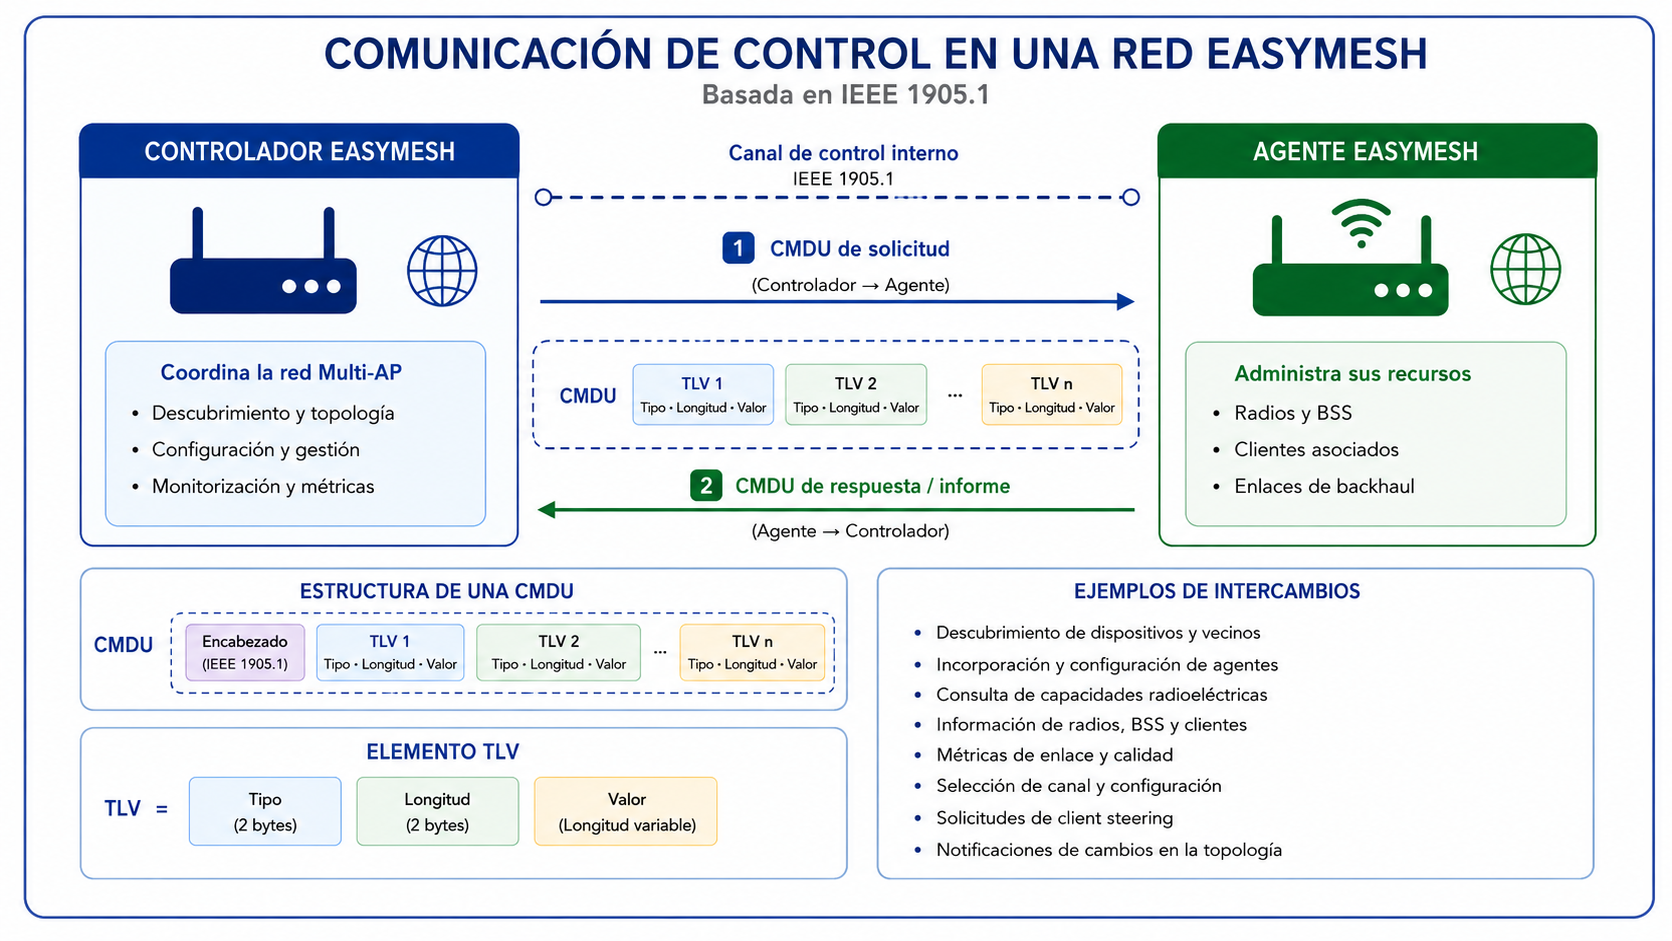
\includegraphics[width=0.90\textwidth]
    {figures/comunicacion_controlador_agentes.png}

    \caption[Comunicación interna entre el controlador y los agentes
    EasyMesh.]
    {Comunicación interna entre el controlador y los agentes EasyMesh.
    El intercambio se realiza mediante mensajes CMDU que contienen
    elementos TLV. El controlador envía consultas y acciones de
    configuración, mientras que los agentes transmiten respuestas,
    métricas y notificaciones relacionadas con el estado de la red.
    \textit{Fuente: imagen generada mediante ChatGPT (OpenAI) a partir
    de las indicaciones de la autora y basada en la especificación
    Wi-Fi EasyMesh y en IEEE~1905.1
    \cite{wifi_alliance_easymesh,ieee_1905_1}.}}

    \label{fig:comunicacion-controlador-agentes}
\end{figure}

La comunicación interna no implica que toda la información intercambiada
quede disponible automáticamente para una plataforma de monitorización
externa. Los mensajes CMDU pertenecen al funcionamiento interno de la red
EasyMesh y no constituyen parámetros que el ACS pueda consultar
directamente.

Para proporcionar visibilidad externa, el controlador debe
\textbf{recopilar, procesar y representar} la información recibida de los
agentes mediante un modelo de datos accesible desde el CPE. En el
presente proyecto, esta representación se obtiene principalmente mediante
TR-181.

También debe considerarse la diferencia entre el
\textbf{instante en el que el agente detecta un evento} y el
\textbf{instante en el que la plataforma externa puede observarlo}. El
primer instante corresponde al funcionamiento interno de EasyMesh,
mientras que el segundo incorpora los retardos asociados a la
actualización del modelo de datos y a la posterior adquisición mediante
TR-069/CWMP.

Por ejemplo, un agente puede detectar inmediatamente que un cliente ha
cambiado de punto de acceso y comunicarlo al controlador. Sin embargo, la
plataforma de gestión solo observa el cambio cuando el CPE actualiza el
parámetro correspondiente y este se consulta o se transmite al ACS.

En el laboratorio desarrollado, la comunicación interna se produce entre
el controlador y los agentes implementados por los dispositivos TP-Link
HX141. GenieACS no participa en este intercambio ni consulta directamente
las CMDU transmitidas dentro de la red.

La plataforma obtiene la información después de que el controlador la
incorpore al árbol de parámetros del CPE. Por tanto, la
\textbf{visibilidad externa depende de la correspondencia entre la
información interna de EasyMesh y los parámetros expuestos mediante
TR-181}.

Esta dependencia explica que la conectividad de la red pueda mantenerse
correctamente aunque la plataforma presente información incompleta o
desactualizada. El funcionamiento interno entre controlador y agentes y
la representación disponible para el ACS constituyen niveles diferentes
de la arquitectura.

En consecuencia, el análisis de la comunicación interna permite
comprender el origen de la información EasyMesh y diferenciarlo del
mecanismo utilizado posteriormente para su monitorización. IEEE~1905.1 y
EasyMesh coordinan la red dentro del domicilio, mientras que TR-181 y
TR-069/CWMP proporcionan la representación y el acceso remoto utilizados
por la plataforma.

\subsection{Información intercambiada en la red Mesh}
\label{subsec:informacion-intercambiada-red-mesh}

El funcionamiento coordinado de una red EasyMesh requiere que el
controlador y los agentes intercambien información sobre los elementos
que forman la infraestructura y sobre los el
controlador y los agentes intercambien información sobre cambios producidos durante su
operación. Esta comunicación permite mantener una
\textbf{representación actualizada de la topología}, conocer las
capacidades de los dispositivos y aplicar las acciones necesarias para
gestionar las radios, los puntos de acceso y los clientes
\cite{wifi_alliance_easymesh,ieee_1905_1}.

La información se transporta mediante los mensajes de control utilizados
por IEEE~1905.1 y EasyMesh. Estos mensajes se organizan mediante
\textbf{CMDU} (\textit{Control Message Data Unit}) y contienen elementos
\textbf{TLV} (\textit{Type-Length-Value}) que representan los distintos
datos intercambiados entre los dispositivos.

El contenido concreto depende del procedimiento ejecutado y de las
funciones implementadas por cada equipo. De forma general, la información
intercambiada puede agruparse en los siguientes ámbitos:

\begin{itemize}
    \item información de \textbf{identificación y descubrimiento};
    \item información de \textbf{topología};
    \item información sobre las \textbf{capacidades de los agentes};
    \item información de \textbf{configuración y estado de las radios};
    \item información sobre los \textbf{BSS y puntos de acceso};
    \item información sobre los \textbf{clientes asociados};
    \item métricas de los enlaces de \textit{fronthaul} y
    \textit{backhaul};
    \item información relacionada con \textit{roaming},
    \textit{steering} y eventos de la red.
\end{itemize}


\subsubsection*{Identificación y descubrimiento de dispositivos}

La información de \textbf{identificación y descubrimiento} permite
detectar los dispositivos compatibles presentes en la red y distinguir
las interfaces pertenecientes a cada uno de ellos. Este intercambio
constituye la base para construir una visión conjunta de la
infraestructura.

Cada dispositivo IEEE~1905.1 dispone de un identificador lógico que
permite reconocerlo dentro de la red con independencia de las
direcciones asociadas a sus interfaces físicas. A partir de este
identificador, el controlador puede diferenciar los dispositivos
Multi-AP y relacionarlos con sus correspondientes agentes.

La información de descubrimiento permite conocer:

\begin{itemize}
    \item la identidad del dispositivo;
    \item las interfaces de red disponibles;
    \item las tecnologías utilizadas por dichas interfaces;
    \item los dispositivos vecinos detectados;
    \item los enlaces existentes entre los distintos nodos.
\end{itemize}

Estos datos permiten determinar si un agente mantiene una conexión
directa con el dispositivo principal o si utiliza otro nodo intermedio
para alcanzar el controlador.


\subsubsection*{Información de topología}

La \textbf{información de topología} describe la organización de los
dispositivos y los enlaces que forman la red mallada. Su finalidad
consiste en representar las relaciones existentes entre el controlador,
los agentes y las interfaces utilizadas para el
\textit{backhaul}.

Entre los datos relevantes se encuentran:

\begin{itemize}
    \item los dispositivos que forman la red Multi-AP;
    \item las interfaces asociadas a cada dispositivo;
    \item los enlaces entre dispositivos vecinos;
    \item el tipo de tecnología utilizada en cada enlace;
    \item el nodo superior de cada agente;
    \item la trayectoria empleada para alcanzar el nodo principal.
\end{itemize}

Esta información permite distinguir entre una
\textbf{topología en estrella}, en la que los agentes se conectan
directamente con el nodo principal, y una
\textbf{topología en cascada}, en la que uno o varios agentes utilizan
nodos intermedios.

La topología puede cambiar durante el funcionamiento de la red. La
desconexión de un nodo, la pérdida de un enlace o la selección de una
nueva trayectoria de \textit{backhaul} pueden modificar las relaciones
entre los dispositivos. Por este motivo, la información debe actualizarse
cuando se detecta un cambio relevante.


\subsubsection*{Capacidades de los agentes}

El controlador necesita conocer las
\textbf{capacidades implementadas por cada agente} antes de aplicar una
configuración o solicitar una determinada operación. Los dispositivos
pueden admitir diferentes bandas, canales, anchos de canal, generaciones
de Wi-Fi y funciones opcionales.

La información sobre capacidades puede incluir:

\begin{itemize}
    \item el número de radios disponibles;
    \item las bandas de frecuencia admitidas;
    \item los canales y anchos de canal soportados;
    \item los estándares IEEE~802.11 implementados;
    \item el número de flujos espaciales;
    \item las capacidades de transmisión y recepción;
    \item las funciones de gestión y monitorización admitidas;
    \item los mecanismos de \textit{steering} compatibles.
\end{itemize}

El intercambio de capacidades evita que el controlador solicite
operaciones que el agente no puede ejecutar. También permite adaptar la
configuración a las características reales de cada dispositivo.


\subsubsection*{Configuración y estado de las radios}

La información de \textbf{radio} permite conocer y gestionar las
interfaces inalámbricas administradas por los agentes. Cada radio puede
operar en una banda determinada y utilizar una configuración específica
de canal, ancho de canal y potencia.

Entre los parámetros que pueden intercambiarse se encuentran:

\begin{itemize}
    \item el identificador de la radio;
    \item la banda de frecuencia;
    \item el canal de operación;
    \item el ancho de canal;
    \item la potencia de transmisión;
    \item el estado operativo;
    \item los canales permitidos o restringidos;
    \item las preferencias de selección de canal;
    \item la utilización observada del medio.
\end{itemize}

El controlador utiliza esta información para mantener una visión
coordinada de los recursos radioeléctricos. A partir de ella puede aplicar
decisiones relacionadas con la selección de canales, la configuración de
las radios o la distribución de los puntos de acceso.


\subsubsection*{Información sobre BSS y puntos de acceso}

Los agentes comunican información sobre los
\textbf{BSS configurados en sus radios}. Esta información permite
identificar los puntos de acceso disponibles y determinar la función que
desempeñan dentro de la red.

Los datos intercambiados pueden incluir:

\begin{itemize}
    \item el identificador de la radio;
    \item el \textbf{BSSID};
    \item el \textbf{SSID};
    \item el estado habilitado o deshabilitado;
    \item la configuración de seguridad;
    \item la función de \textit{fronthaul} o
    \textit{backhaul};
    \item el número de clientes asociados.
\end{itemize}

La relación entre el BSSID, la radio y el agente resulta necesaria para
determinar el punto de acceso concreto que proporciona conectividad a
cada cliente.

Varios BSS pueden anunciar el mismo SSID y formar parte de una única red
lógica. Sin embargo, cada BSS mantiene un BSSID diferente, por lo que el
SSID no resulta suficiente para identificar el nodo de asociación.


\subsubsection*{Información sobre clientes asociados}

La información de \textbf{clientes asociados} permite mantener una visión
actualizada de las estaciones Wi-Fi conectadas a los diferentes puntos
de acceso.

Entre los datos que pueden comunicarse se encuentran:

\begin{itemize}
    \item la dirección MAC del cliente;
    \item el BSSID utilizado;
    \item la radio y el agente correspondientes;
    \item el estado de asociación;
    \item el tiempo de permanencia en el BSS;
    \item las capacidades del terminal;
    \item los contadores de tráfico;
    \item determinadas métricas de calidad radio.
\end{itemize}

La dirección MAC permite identificar al cliente con independencia del
BSS al que se encuentra asociado. Esta característica resulta esencial
cuando el dispositivo cambia entre el controlador y los agentes o entre
dos agentes diferentes.

Cuando se produce un cambio de asociación, el cliente deja de aparecer
en el BSS de origen y pasa a formar parte del BSS de destino. La
actualización de esta información permite reconstruir la movilidad del
terminal dentro de la red mallada.


\subsubsection*{Métricas de enlace}

Los agentes pueden proporcionar
\textbf{métricas relacionadas con los enlaces} utilizados por los
clientes y por los propios nodos. Estas métricas permiten evaluar las
condiciones del \textit{fronthaul} y del \textit{backhaul}.

En el enlace entre el cliente y el punto de acceso pueden resultar
relevantes:

\begin{itemize}
    \item el nivel de señal;
    \item las tasas físicas de transmisión y recepción;
    \item los bytes y paquetes transferidos;
    \item los errores de transmisión;
    \item las retransmisiones;
    \item la duración de la asociación.
\end{itemize}

En los enlaces de \textit{backhaul} pueden intercambiarse datos sobre:

\begin{itemize}
    \item los dispositivos situados en cada extremo;
    \item la interfaz utilizada;
    \item el tipo de enlace;
    \item el estado operativo;
    \item la capacidad estimada;
    \item la calidad radioeléctrica;
    \item la trayectoria hasta el nodo principal.
\end{itemize}

La interpretación conjunta de estas métricas permite diferenciar una
degradación producida en el enlace de acceso del cliente de otra
originada en la comunicación entre los agentes.


\subsubsection*{Información de movilidad y \textit{steering}}

La gestión de los clientes requiere intercambiar información relacionada
con las operaciones de \textbf{\textit{client steering}} y con los
cambios de asociación observados en la red.

El controlador puede obtener información sobre:

\begin{itemize}
    \item el cliente afectado;
    \item el BSSID de origen;
    \item los BSSID candidatos;
    \item el BSSID de destino recomendado;
    \item la causa de la operación;
    \item el resultado de la solicitud;
    \item la asociación finalmente observada.
\end{itemize}

Una solicitud de \textit{steering} representa una actuación de la red,
pero no garantiza que el cliente realice la transición. El terminal puede
aceptar, posponer o rechazar la recomendación según sus propios
mecanismos de selección.

Por este motivo, el controlador debe diferenciar entre la
\textbf{acción solicitada} y el
\textbf{cambio efectivo de asociación}. La confirmación del cambio
requiere observar al cliente en el BSS de destino.


\subsubsection*{Notificaciones y cambios de estado}

Además de responder a consultas, los agentes pueden comunicar
\textbf{eventos y cambios de estado} detectados durante el funcionamiento
de la red.

Estas notificaciones pueden estar relacionadas con:

\begin{itemize}
    \item la incorporación o desconexión de un agente;
    \item la aparición o pérdida de un enlace;
    \item la conexión o desconexión de un cliente;
    \item un cambio de asociación;
    \item una modificación de canal;
    \item una variación en el estado operativo de una radio;
    \item el resultado de una acción de configuración.
\end{itemize}

Las notificaciones permiten que el controlador actualice su
representación de la red sin depender exclusivamente de consultas
periódicas. Sin embargo, la disponibilidad y el detalle de los eventos
dependen de las funciones implementadas por los dispositivos.


\subsubsection*{Relación con la monitorización externa}

La información intercambiada dentro de la red EasyMesh pertenece al
\textbf{plano interno de control}. Su existencia no implica que pueda
consultarse directamente desde una plataforma externa.

GenieACS no recibe las CMDU ni interpreta los TLV intercambiados entre el
controlador y los agentes. El ACS únicamente puede acceder a los
parámetros que el CPE incorpora a su modelo de datos y expone mediante
TR-069/CWMP.

La cadena de información puede representarse de forma simplificada como:

\[
    \text{Agentes}
    \xrightarrow{\text{IEEE~1905.1/EasyMesh}}
    \text{Controlador}
    \xrightarrow{\text{TR-181}}
    \text{CPE}
    \xrightarrow{\text{TR-069/CWMP}}
    \text{ACS}.
\]

En esta secuencia, IEEE~1905.1 y EasyMesh permiten recopilar y comunicar
la información dentro de la vivienda. TR-181 proporciona la estructura
utilizada para representarla, mientras que TR-069/CWMP permite que el ACS
consulte los parámetros expuestos por el CPE.

No toda la información disponible internamente tiene que aparecer en
TR-181. La visibilidad externa depende de:

\begin{itemize}
    \item los datos recopilados por el controlador;
    \item la información que el firmware incorpora al modelo de datos;
    \item los parámetros realmente expuestos por el CPE;
    \item la frecuencia con la que se actualizan dichos parámetros;
    \item el procedimiento empleado para consultarlos desde el ACS.
\end{itemize}

Por tanto, puede existir una diferencia entre el
\textbf{estado interno conocido por EasyMesh} y el
\textbf{estado observable desde la plataforma de gestión}. La red puede
mantener correctamente la conectividad de un cliente mientras el ACS
dispone de una asociación incompleta o desactualizada.

En el laboratorio desarrollado, esta diferencia resulta especialmente
importante durante las pruebas de movilidad. Los agentes y el controlador
pueden detectar internamente el cambio de nodo, pero la plataforma solo
lo observa cuando el CPE actualiza la información correspondiente y esta
se obtiene mediante TR-069/CWMP.

En consecuencia, el análisis de la información intercambiada en la red
Mesh permite identificar el origen de la telemetría y comprender las
limitaciones de su posterior exposición. Para mantener la trazabilidad
del cliente, la plataforma necesita que la información sobre
\textbf{topología}, \textbf{radios}, \textbf{BSS},
\textbf{clientes} y \textbf{enlaces} se represente de forma coherente,
estable y suficientemente actualizada.

\subsection{Diferencia entre IEEE 1905.1, TR-069 y TR-181}
\label{subsec:diferencia-ieee1905-tr069-tr181}

La monitorización de una red EasyMesh implica la utilización de
diferentes tecnologías que actúan en niveles distintos de la
arquitectura. En particular, deben diferenciarse
\textbf{IEEE~1905.1}, \textbf{TR-069/CWMP} y
\textbf{TR-181}, ya que cada uno desempeña una función específica y no
pueden interpretarse como mecanismos equivalentes.

IEEE~1905.1 proporciona una
\textbf{capa de abstracción y comunicación interna} para redes domésticas
formadas por tecnologías heterogéneas. TR-069/CWMP define un
\textbf{protocolo de gestión remota} entre un CPE y un ACS. Por su parte,
TR-181 establecetextbf{protocolo de gestión remota} entre un CPE un \textbf{modelo de datos} compuesto por objetos y
parámetros que representan la configuración, el estado y las
capacidades del dispositivo
\cite{ieee_1905_1,bbf_tr069,bbf_tr181}.

Por tanto, la diferencia fundamental puede expresarse de la siguiente
forma:

\begin{itemize}
    \item \textbf{IEEE~1905.1 comunica y coordina los dispositivos
    dentro de la red doméstica}.

    \item \textbf{TR-069/CWMP permite gestionar remotamente el CPE desde
    un ACS}.

    \item \textbf{TR-181 define cómo se estructura la información que
    expone el dispositivo}.
\end{itemize}


\subsubsection*{IEEE~1905.1 como mecanismo interno de comunicación}

IEEE~1905.1 define una capa de abstracción situada funcionalmente entre
la capa de enlace y la capa de red. Esta capa proporciona una interfaz
común para representar dispositivos e interfaces pertenecientes a
tecnologías como Wi-Fi, Ethernet, redes sobre líneas eléctricas y
conexiones sobre cable coaxial \cite{ieee_1905_1}.

Su ámbito de funcionamiento corresponde principalmente a la
\textbf{red interna del domicilio}. Los dispositivos compatibles
intercambian mensajes destinados al descubrimiento de nodos, la
representación de la topología, la identificación de interfaces y la
obtención de información sobre los enlaces existentes.

En una red EasyMesh, IEEE~1905.1 proporciona la base utilizada para la
\textbf{comunicación entre el controlador y los agentes}. Sobre esta
capa, la especificación EasyMesh incorpora procedimientos específicos
para configurar los puntos de acceso, consultar capacidades, recopilar
métricas y gestionar los clientes de la infraestructura Multi-AP
\cite{wifi_alliance_easymesh,ieee_1905_1}.

La comunicación se realiza mediante mensajes CMDU que contienen
elementos TLV. Estos mensajes circulan entre los dispositivos que forman
la red mallada y permiten transportar información sobre la topología,
las radios, los BSS, los clientes y los enlaces de
\textit{backhaul}.

IEEE~1905.1 no establece por sí mismo una sesión de gestión entre el
domicilio y la plataforma del operador. Tampoco define un árbol de
parámetros equivalente a \texttt{Device}. Su función se concentra en la
\textbf{comunicación y coordinación interna de los dispositivos de la
red doméstica}.


\subsubsection*{TR-069/CWMP como protocolo de gestión remota}

TR-069 define el
\textbf{CPE WAN Management Protocol o CWMP}, utilizado para establecer la
comunicación entre un CPE y un servidor de autoconfiguración o ACS
\cite{bbf_tr069}.

A diferencia de IEEE~1905.1, TR-069 actúa entre la
\textbf{red residencial y la plataforma externa de gestión}. Su finalidad
consiste en permitir que el operador configure, consulte, diagnostique y
mantenga remotamente los dispositivos instalados en las dependencias del
cliente.

La relación funcional se establece entre dos entidades:

\begin{itemize}
    \item el \textbf{CPE}, que contiene los parámetros y establece la
    comunicación con la plataforma;

    \item el \textbf{ACS}, que solicita operaciones de consulta,
    configuración o diagnóstico sobre el dispositivo.
\end{itemize}

TR-069 define los procedimientos utilizados para establecer las
\textbf{sesiones CWMP} y ejecutar operaciones remotas. Entre estas
operaciones se encuentran la notificación del estado del dispositivo, la
consulta de parámetros, la modificación de valores, la descarga de
archivos y la ejecución de determinados diagnósticos.

El protocolo no determina por sí solo qué parámetros Wi-Fi, EasyMesh o
de red debe contener un equipo. TR-069 proporciona el
\textbf{mecanismo de transporte y gestión}, mientras que la organización
de los parámetros se establece mediante un modelo de datos compatible,
como TR-181.

Esta separación permite que el mismo protocolo se utilice con diferentes
tipos de dispositivos y versiones del modelo de datos. El ACS consulta
rutas concretas, pero el significado, el tipo y la estructura de dichas
rutas se encuentran definidos fuera del protocolo CWMP.


\subsubsection*{TR-181 como modelo de datos}

TR-181 define el
\textbf{modelo de datos Device:2}, utilizado para representar las
funciones y capacidades de dispositivos de red, como pasarelas
residenciales, CPE y otros equipos gestionables
\cite{bbf_tr181}.

El modelo se organiza mediante un
\textbf{árbol jerárquico de objetos y parámetros} cuya raíz se identifica
como:

\[
    \texttt{Device.}
\]

A partir de esta raíz se definen ramas destinadas a representar
información sobre el propio equipo, las interfaces, la conectividad IP,
el encaminamiento, Ethernet, Wi-Fi, los dispositivos asociados, los
diagnósticos y otras funciones.

Por ejemplo, la información inalámbrica puede aparecer dentro de rutas
como:

\[
    \texttt{Device.WiFi.}
\]

La representación de elementos relacionados con redes Multi-AP puede
incorporarse mediante:

\[
    \texttt{Device.WiFi.DataElements.}
\]

TR-181 no establece directamente una comunicación entre dispositivos.
Tampoco consulta por sí mismo las radios, los agentes o los clientes. El
modelo únicamente define la \textbf{estructura, el significado y el tipo
de los datos que puede exponer el equipo}.

El firmware del CPE es responsable de recopilar la información interna,
actualizar los objetos correspondientes y proporcionar los valores
cuando son solicitados mediante un protocolo de gestión.

En el contexto de este proyecto, TR-181 representa el
\textbf{punto de unión entre el funcionamiento interno de EasyMesh y la
gestión remota mediante TR-069}. La información obtenida por el
controlador debe incorporarse a las ramas correspondientes del modelo
antes de que GenieACS pueda consultarla.


\subsubsection*{Relación funcional entre los tres mecanismos}

La relación completa puede representarse mediante la siguiente cadena:

\[
\boxed{
\begin{gathered}
\text{Agentes EasyMesh}
\overset{\text{IEEE~1905.1 / EasyMesh}}{\longleftrightarrow}
\text{Controlador integrado en el CPE}
\\[0.2cm]
\text{Controlador integrado en el CPE}
\overset{\text{TR-181}}{\longrightarrow}
\text{Árbol de parámetros del CPE}
\\[0.2cm]
\text{Árbol de parámetros del CPE}
\overset{\text{TR-069/CWMP}}{\longleftrightarrow}
\text{ACS}
\end{gathered}
}
\]

En la primera etapa, IEEE~1905.1 y EasyMesh permiten que el controlador
reciba información de los agentes y mantenga una visión coordinada de la
topología.

En la segunda etapa, el firmware del CPE transforma o incorpora esa
información a los objetos y parámetros definidos por TR-181.

En la tercera etapa, TR-069/CWMP permite que el ACS consulte los
parámetros expuestos por el CPE y almacene una representación remota del
estado del dispositivo.

Por tanto, los tres mecanismos actúan de forma complementaria:

\[
    \underbrace{\text{IEEE~1905.1}}_{\text{comunicación interna}}
    \quad+\quad
    \underbrace{\text{TR-181}}_{\text{representación de datos}}
    \quad+\quad
    \underbrace{\text{TR-069/CWMP}}_{\text{gestión remota}}
\]


\subsubsection*{Comparación de funciones}

La Tabla~\ref{tab:diferencias-ieee1905-tr069-tr181} resume las
principales diferencias entre los tres mecanismos.

\begin{table}[H]
    \centering
    \small
    \renewcommand{\arraystretch}{1.35}

    \caption[Diferencias entre IEEE~1905.1, TR-069/CWMP y TR-181.]
    {Diferencias funcionales entre IEEE~1905.1, TR-069/CWMP y TR-181.
    \textit{Fuente: elaboración propia a partir de IEEE~1905.1 y de las
    especificaciones del Broadband Forum
    \cite{ieee_1905_1,bbf_tr069,bbf_tr181}.}}

    \label{tab:diferencias-ieee1905-tr069-tr181}

    \begin{tabular}{
        p{0.15\textwidth}
        p{0.25\textwidth}
        p{0.25\textwidth}
        p{0.25\textwidth}
    }
        \hline
        \textbf{Aspecto}
        &
        \textbf{IEEE~1905.1}
        &
        \textbf{TR-069/CWMP}
        &
        \textbf{TR-181}
        \\
        \hline

        Tipo
        &
        Capa de abstracción y comunicación.
        &
        Protocolo de gestión remota.
        &
        Modelo de datos jerárquico.
        \\

        Ámbito
        &
        Interior de la red doméstica.
        &
        Comunicación entre el CPE y el ACS.
        &
        Representación de funciones y parámetros del dispositivo.
        \\

        Entidades
        &
        Dispositivos, interfaces y vecinos IEEE~1905.1.
        &
        CPE y ACS.
        &
        Objetos y parámetros bajo la raíz \texttt{Device.}
        \\

        Función principal
        &
        Descubrimiento, topología e intercambio interno de información.
        &
        Consulta, configuración, diagnóstico y mantenimiento remoto.
        &
        Organización de la configuración, el estado y la telemetría.
        \\

        En EasyMesh
        &
        Transporta la comunicación interna entre controlador y agentes.
        &
        Permite gestionar remotamente el CPE que contiene el controlador.
        &
        Representa agentes, radios, BSS, clientes y otras funciones.
        \\

        Unidad de información
        &
        Mensajes CMDU y elementos TLV.
        &
        Sesiones CWMP y llamadas RPC.
        &
        Objetos, tablas y parámetros.
        \\

        Acceso desde el ACS
        &
        No se consulta directamente.
        &
        Constituye el protocolo utilizado por el ACS.
        &
        Se consulta mediante las rutas expuestas por el CPE.
        \\

        Dependencia del firmware
        &
        Implementación interna de IEEE~1905.1 y EasyMesh.
        &
        Implementación del cliente CWMP.
        &
        Objetos y parámetros realmente implementados y actualizados.
        \\

        Ejemplo
        &
        Descubrimiento de un agente EasyMesh.
        &
        Ejecución de \texttt{GetParameterValues}.
        &
        Consulta de \texttt{Device.WiFi.DataElements.}
        \\

        \hline
    \end{tabular}
\end{table}

\subsubsection*{Diferencia entre información interna y observable}

La existencia de información dentro de IEEE~1905.1 no garantiza que
dicha información resulte visible mediante TR-181. El controlador puede
conocer internamente la asociación de un cliente o la calidad de un
enlace de \textit{backhaul}, pero el firmware debe trasladar esos datos
al modelo antes de que puedan consultarse remotamente.

Del mismo modo, la presencia de un parámetro dentro del árbol TR-181 no
garantiza que su valor se actualice inmediatamente. La frecuencia de
actualización depende de la implementación del fabricante y del
procedimiento utilizado por el CPE para incorporar la información
procedente de la red EasyMesh.

Finalmente, aunque el parámetro se encuentre actualizado en el CPE, el
ACS no recibe necesariamente el cambio de manera instantánea. La
plataforma debe obtenerlo durante una sesión CWMP, mediante una consulta
explícita o a través del mecanismo de notificación configurado.

Por tanto, pueden distinguirse tres instantes:

\begin{enumerate}
    \item el instante en el que se produce el
    \textbf{evento dentro de la red EasyMesh};

    \item el instante en el que el firmware
    \textbf{actualiza el parámetro TR-181};

    \item el instante en el que el ACS
    \textbf{obtiene el valor mediante TR-069/CWMP}.
\end{enumerate}

La diferencia temporal entre estos instantes explica por qué el momento
observado en la plataforma puede no coincidir con el instante exacto en
el que se produce un cambio radio o una modificación de la topología.


\subsubsection*{Aplicación en el laboratorio desarrollado}

En el laboratorio del presente proyecto, los agentes TP-Link HX141
intercambian información con el controlador mediante los mecanismos
internos de EasyMesh e IEEE~1905.1. Este intercambio permite mantener la
topología de la red y conocer los clientes asociados a los diferentes
nodos.

El controlador se encuentra integrado en el CPE principal. El firmware
del equipo representa parte de la información de la red mediante el
modelo TR-181, principalmente dentro de la rama:

\[
    \texttt{Device.WiFi.DataElements.}
\]

GenieACS actúa como ACS y se comunica con el CPE mediante TR-069/CWMP. La
plataforma no recibe directamente los mensajes IEEE~1905.1 ni consulta a
los agentes como CPE independientes.

En consecuencia, el flujo de información utilizado en el laboratorio es:

\[
    \text{Agentes}
    \xrightarrow{\text{IEEE~1905.1 / EasyMesh}}
    \text{Controlador}
    \xrightarrow{\text{TR-181}}
    \text{CPE}
    \xrightarrow{\text{TR-069/CWMP}}
    \text{GenieACS}.
\]

Esta arquitectura implica que la
\textbf{observabilidad externa depende de toda la cadena}. Una pérdida de
información, una actualización tardía o una implementación incompleta en
cualquiera de sus etapas puede provocar que GenieACS mantenga una visión
parcial o desactualizada de la red.

Por tanto, IEEE~1905.1, TR-181 y TR-069/CWMP no compiten entre sí, sino
que desempeñan funciones complementarias:

\begin{itemize}
    \item IEEE~1905.1 proporciona la
    \textbf{visibilidad y comunicación internas};

    \item TR-181 proporciona la
    \textbf{representación estructurada de la información};

    \item TR-069/CWMP proporciona el
    \textbf{acceso remoto desde la plataforma de gestión}.
\end{itemize}

La correcta integración de estos tres mecanismos permite trasladar el
estado interno de la red EasyMesh hasta la plataforma de monitorización.
Cuando esta integración resulta incompleta, aparece el punto ciego de
visibilidad que motiva el desarrollo del presente proyecto.

\section{TR-181}
\label{sec:tr-181}

La gestión y monitorización de un dispositivo de red requieren una
representación estructurada de sus funciones, capacidades, parámetros de
configuración y variables de estado. Sin un modelo común, cada fabricante
podría utilizar nombres, jerarquías y formatos diferentes, lo que
dificultaría la interoperabilidad con las plataformas de gestión.

El Broadband Forum define \textbf{TR-181} como el modelo de datos
\textbf{Device:2}, aplicable a dispositivos compatibles con TR-069/CWMP
o USP. Este modelo permite representar diferentes tipos de equipos,
entre ellos terminales, pasarelas residenciales y dispositivos de
infraestructura de red \cite{bbf_tr181}.

TR-181 no constituye un protocolo de comunicación. Su función consiste
en definir una \textbf{estructura jerárquica de objetos y parámetros}
que describe las capacidades y el estado del dispositivo. El acceso a
dicha estructura se realiza mediante un protocolo de gestión, como
TR-069/CWMP o USP.

En el contexto del presente proyecto, TR-181 se utiliza junto con
\textbf{TR-069/CWMP}. El modelo de datos determina qué información puede
representar el CPE, mientras que TR-069 establece el mecanismo mediante
el cual GenieACS solicita, recibe o modifica los valores expuestos por el
equipo.

La raíz del modelo Device:2 se identifica mediante el objeto:

\[
    \texttt{Device.}
\]

A partir de esta raíz se organizan diferentes ramas destinadas a
representar la identificación del equipo, las interfaces de red, la
conectividad IP, el encaminamiento, Ethernet, Wi-Fi, los dispositivos
conectados, los mecanismos de gestión, las estadísticas y las
operaciones de diagnóstico \cite{bbf_tr181}.

La organización jerárquica permite agrupar parámetros relacionados dentro
de un mismo objeto. Por ejemplo, la información correspondiente a la
conectividad inalámbrica se organiza principalmente bajo la rama:

\[
    \texttt{Device.WiFi.}
\]

Dentro de esta estructura pueden representarse las radios, los SSID, los
puntos de acceso, los clientes asociados y diferentes parámetros de
configuración y estado relacionados con la red inalámbrica.

Los elementos del modelo pueden clasificarse en
\textbf{objetos}, \textbf{tablas}, \textbf{instancias} y
\textbf{parámetros}. Los objetos agrupan información relacionada,
mientras que las tablas permiten representar conjuntos variables de
elementos, como interfaces, radios, puntos de acceso o estaciones
asociadas.

Cada elemento contenido en una tabla se identifica mediante un número de
\textbf{instancia}. De forma genérica, una ruta puede representarse como:

\[
    \texttt{Device.Objeto.\{i\}.Parametro}
\]

donde \texttt{\{i\}} representa la instancia concreta del elemento
consultado. Por ejemplo, distintas radios Wi-Fi pueden aparecer como
instancias separadas dentro de la tabla correspondiente.

Los parámetros representan los valores finales del modelo. Cada
parámetro dispone de un nombre, un tipo de dato, unas condiciones de
acceso y una descripción semántica. Dependiendo de su definición, puede
ser de \textbf{solo lectura} o permitir también su
\textbf{modificación desde la plataforma de gestión}.

Los parámetros de solo lectura permiten consultar información como el
estado operativo, los contadores de tráfico o determinados valores
medidos por el dispositivo. Los parámetros modificables permiten aplicar
configuraciones, siempre que el firmware implemente la operación y el
usuario de gestión disponga de los permisos necesarios.

TR-181 incorpora además un mecanismo de
\textbf{apilamiento de interfaces}. Las interfaces y las capas de
protocolo se representan mediante objetos independientes que pueden
relacionarse a través de referencias entre capas superiores e
inferiores. Este mecanismo permite describir configuraciones de red
formadas por varias tecnologías superpuestas \cite{bbf_tr181}.

Por ejemplo, una interfaz IP puede utilizar una interfaz Ethernet o
Wi-Fi como capa inferior. A su vez, una interfaz Wi-Fi puede
corresponder a un SSID configurado sobre una radio física. Esta
separación permite representar de manera estructurada la trayectoria
lógica seguida por la conectividad dentro del dispositivo.

El modelo también utiliza referencias entre objetos para establecer
relaciones. Un parámetro puede contener la ruta de otro elemento del árbol
y permitir así la asociación entre una interfaz, una radio, un punto de
acceso o un cliente.

Esta característica resulta relevante en redes Wi-Fi, donde es necesario
diferenciar entre:

\begin{itemize}
    \item la \textbf{radio física};
    \item el \textbf{SSID configurado};
    \item el \textbf{punto de acceso};
    \item el \textbf{BSSID};
    \item las \textbf{estaciones asociadas}.
\end{itemize}

La existencia de estos niveles permite representar con mayor precisión la
infraestructura inalámbrica. Sin embargo, también obliga a correlacionar
varias ramas del modelo para determinar qué radio y qué punto de acceso
proporcionan servicio a cada cliente.

Para representar información relacionada con redes formadas por varios
puntos de acceso, TR-181 incorpora la estructura:

\[
    \texttt{Device.WiFi.DataElements.}
\]

Esta rama permite organizar información sobre los dispositivos que
forman la red, sus radios, los BSS configurados y las estaciones
asociadas. Su estructura resulta especialmente relevante para la
observación de una topología EasyMesh y se desarrolla posteriormente en
el Apartado~\ref{subsec:device-wifi-dataelements}.

TR-181 también define la rama:

\[
    \texttt{Device.BulkData.}
\]

Esta estructura permite configurar perfiles destinados a recopilar y
enviar conjuntos de parámetros de forma periódica. Su finalidad consiste
en facilitar la generación de informes de telemetría sin depender
exclusivamente de consultas individuales realizadas por la plataforma.
Este mecanismo se analiza en el
Apartado~\ref{subsec:device-bulkdata} y en la
Sección~\ref{sec:bulkdata}.

Debe distinguirse entre los
\textbf{parámetros definidos por TR-181} y los
\textbf{parámetros realmente implementados por un dispositivo}. El
modelo especifica un conjunto amplio de objetos, pero un fabricante puede
implementar únicamente aquellos que resultan aplicables al equipo y a
las funciones proporcionadas por su firmware.

Por tanto, la presencia de un objeto en la especificación no garantiza
que aparezca en el árbol de parámetros del CPE. Del mismo modo, la
existencia de un parámetro en el dispositivo no garantiza que su valor se
encuentre actualizado, documentado o disponible con la periodicidad
necesaria para la monitorización.

Los fabricantes también pueden incorporar
\textbf{extensiones propietarias} para representar funciones no cubiertas
por el modelo normalizado. Estas extensiones utilizan identificadores
específicos del proveedor y pueden dificultar la portabilidad de una
plataforma entre dispositivos de diferentes fabricantes.

Desde el punto de vista de la monitorización, deben verificarse al menos
los siguientes aspectos:

\begin{itemize}
    \item la \textbf{existencia del objeto o parámetro};
    \item el \textbf{tipo de dato} proporcionado;
    \item la \textbf{unidad} utilizada;
    \item su condición de \textbf{lectura o escritura};
    \item la \textbf{frecuencia de actualización};
    \item la estabilidad de las \textbf{instancias};
    \item la correspondencia con el estado real de la red.
\end{itemize}

La estabilidad de las instancias resulta especialmente importante. Un
cliente puede aparecer en una posición diferente después de un cambio de
asociación, una actualización de la topología o un reinicio. Por este
motivo, la plataforma no debe utilizar únicamente el número de instancia
como identificador permanente.

La identidad del cliente debe establecerse mediante un atributo estable,
como su \textbf{dirección MAC}, y relacionarse posteriormente con la
radio, el BSS, el agente y el dispositivo correspondientes. Esta
normalización permite conservar la continuidad de las series temporales
aunque cambie la posición del elemento dentro del árbol TR-181.

También debe considerarse la \textbf{antigüedad de los valores}. El
modelo puede proporcionar una asociación técnicamente válida en el
momento de su actualización, pero dicha información puede quedar
obsoleta después de que el cliente cambie de punto de acceso.

En consecuencia, la interpretación de la telemetría requiere relacionar
cada valor con el instante de adquisición y con el momento de su última
actualización. Esta condición resulta esencial durante los procesos de
movilidad y \textit{roaming}, en los que el estado de asociación puede
cambiar en intervalos reducidos.

En el laboratorio desarrollado, el controlador EasyMesh se encuentra
integrado en el CPE TP-Link HX141. El firmware recopila información sobre
los agentes, las radios, los puntos de acceso y los clientes, y expone
parte de ella mediante el árbol TR-181 del dispositivo.

GenieACS consulta este árbol mediante TR-069/CWMP. Posteriormente, la
información almacenada en el ACS se obtiene mediante la API NBI y se
transforma en métricas compatibles con Prometheus.

El flujo general puede representarse de la siguiente forma:

\[
    \text{Red EasyMesh}
    \longrightarrow
    \text{objetos y parámetros TR-181}
    \longrightarrow
    \text{TR-069/CWMP}
    \longrightarrow
    \text{GenieACS}.
\]

TR-181 constituye, por tanto, la
\textbf{representación estructurada que conecta el estado interno de la
red con la plataforma de gestión}. Su correcta implementación determina
qué elementos pueden observarse, cómo se identifican y con qué nivel de
detalle se encuentran disponibles.

Los apartados siguientes desarrollan TR-181 como modelo de datos, la
estructura del árbol \texttt{Device.}, las ramas relacionadas con Wi-Fi,
los objetos \texttt{Device.WiFi.DataElements} y
\texttt{Device.BulkData}, y su aplicación para representar telemetría de
una red EasyMesh.

\subsection{TR-181 como modelo de datos}
\label{subsec:tr181-modelo-datos}

\textbf{TR-181} define un modelo normalizado para representar las
funciones, capacidades, configuraciones y variables de estado de un
dispositivo de red. Su finalidad consiste en proporcionar una
\textbf{estructura común de información} que pueda ser interpretada por
equipos y plataformas de gestión pertenecientes a implementaciones
diferentes \cite{bbf_tr181}.

El modelo recibe la denominación \textbf{Device:2} y puede aplicarse a
terminales, pasarelas residenciales, CPE y otros dispositivos de
infraestructura compatibles con TR-069/CWMP o USP. En el presente
proyecto, el modelo se utiliza mediante TR-069/CWMP para representar la
información expuesta por el controlador EasyMesh integrado en el CPE.

TR-181 no transporta información por sí mismo. El modelo especifica
\textbf{cómo se organizan y describen los datos}, mientras que el
protocolo de gestión determina cómo se consultan, modifican o notifican
los valores. Por tanto, deben diferenciarse claramente:

\begin{itemize}
    \item el \textbf{modelo de datos TR-181}, que define los objetos y
    parámetros;

    \item el \textbf{protocolo TR-069/CWMP}, que permite acceder
    remotamente a dichos elementos.
\end{itemize}

La información se organiza mediante un
\textbf{árbol jerárquico} cuya raíz corresponde al objeto:

\[
    \texttt{Device.}
\]

A partir de esta raíz se definen ramas destinadas a representar las
diferentes funciones del dispositivo. Cada rama puede contener otros
objetos, tablas, instancias y parámetros, formando rutas que identifican
de manera inequívoca cada elemento del modelo.

Una ruta TR-181 puede expresarse de forma genérica como:

\[
    \texttt{Device.Objeto.Subobjeto.Parametro}
\]

Por ejemplo, las funciones relacionadas con la conectividad inalámbrica
se agrupan bajo la rama:

\[
    \texttt{Device.WiFi.}
\]

Esta organización permite separar la información correspondiente a las
radios, los SSID, los puntos de acceso, las estaciones asociadas y otros
elementos relacionados con el funcionamiento de la red Wi-Fi.

Los componentes principales del modelo son los
\textbf{objetos} y los \textbf{parámetros}. Un objeto agrupa información
relacionada y puede contener otros objetos o parámetros. Un parámetro
representa un valor concreto, como un estado, un contador, un
identificador o una opción de configuración.

Los objetos pueden ser de
\textbf{instancia única} o de \textbf{instancias múltiples}. Un objeto
de instancia única representa un elemento que aparece una sola vez
dentro de su rama. En cambio, un objeto de instancias múltiples actúa
como una tabla capaz de contener un número variable de entradas.

Las tablas se representan mediante un identificador de instancia. De
forma genérica, su estructura se expresa como:

\[
    \texttt{Device.Objeto.\{i\}.Parametro}
\]

donde \texttt{\{i\}} representa el número de la entrada concreta. Por
ejemplo, una tabla de radios puede contener varias instancias:

\[
\begin{aligned}
    &\texttt{Device.WiFi.Radio.1.}\\
    &\texttt{Device.WiFi.Radio.2.}
\end{aligned}
\]

Cada instancia representa una radio diferente, aunque el significado
concreto de su posición depende de la implementación del dispositivo.

El número de instancia permite localizar un elemento dentro del árbol,
pero no debe considerarse necesariamente un
\textbf{identificador permanente}. Después de un reinicio, una
reconfiguración o un cambio en la topología, determinadas tablas pueden
presentar una organización diferente.

Por esta razón, cuando se requiere mantener la trazabilidad de un
elemento, deben utilizarse atributos estables, como una dirección MAC, un
BSSID o un identificador persistente. La instancia numérica se utiliza
para acceder al objeto, pero la identidad lógica debe obtenerse a partir
de los parámetros contenidos en él.

Cada parámetro dispone de un
\textbf{tipo de dato} que determina la forma en la que debe
interpretarse su valor. Entre los tipos habituales se encuentran:

\begin{itemize}
    \item cadenas de texto;
    \item valores booleanos;
    \item enteros con o sin signo;
    \item valores de fecha y hora;
    \item enumeraciones;
    \item referencias hacia otros objetos;
    \item contadores y valores estadísticos.
\end{itemize}

La definición de un parámetro también establece su
\textbf{semántica}, las posibles unidades, los valores admitidos y las
condiciones bajo las que debe encontrarse disponible. Esta información
resulta necesaria para evitar interpretaciones incorrectas durante la
transformación de la telemetría en métricas.

Los parámetros pueden clasificarse según sus permisos de acceso. Un
parámetro de \textbf{solo lectura} permite que la plataforma consulte su
valor, pero no autoriza su modificación. Estos parámetros se utilizan
habitualmente para representar estados, estadísticas, capacidades o
información de identificación.

Un parámetro de \textbf{lectura y escritura} puede modificarse mediante
el protocolo de gestión cuando el dispositivo implementa dicha función.
Este tipo de parámetro se utiliza para aplicar configuraciones, habilitar
servicios o modificar el comportamiento de una interfaz.

La condición de escritura definida por el modelo no garantiza que todas
las operaciones puedan ejecutarse en cualquier dispositivo. El firmware
debe implementar el parámetro y aceptar la modificación solicitada. Del
mismo modo, pueden existir restricciones derivadas del estado operativo,
de los permisos o de la configuración del equipo.

TR-181 utiliza además
\textbf{referencias entre objetos}. Un parámetro puede contener la ruta
de otro elemento del árbol, lo que permite establecer relaciones entre
interfaces, capas de protocolo, radios, SSID, puntos de acceso y otros
componentes.

Estas referencias son necesarias porque un mismo servicio puede estar
formado por varios elementos independientes. Por ejemplo, la
representación de una red inalámbrica puede requerir relacionar:

\[
    \text{Radio}
    \longrightarrow
    \text{SSID}
    \longrightarrow
    \text{Punto de acceso}
    \longrightarrow
    \text{Cliente asociado}.
\]

La existencia de estas relaciones evita representar toda la
infraestructura como un único objeto y permite describir de manera más
precisa la función desempeñada por cada elemento.

Uno de los mecanismos principales de Device:2 es el
\textbf{apilamiento de interfaces}. Las interfaces y las capas de
protocolo se modelan como objetos independientes que pueden relacionarse
para representar la configuración real del dispositivo
\cite{bbf_tr181}.

Mediante este mecanismo puede indicarse, por ejemplo, que una interfaz IP
utiliza una interfaz Ethernet o Wi-Fi como capa inferior. De esta forma,
el modelo representa no solo la presencia de las interfaces, sino también
la relación existente entre ellas.

De manera simplificada, una pila de interfaces puede representarse como:

\[
    \text{Interfaz IP}
    \longrightarrow
    \text{Interfaz de enlace}
    \longrightarrow
    \text{Interfaz física}.
\]

Esta separación facilita la representación de configuraciones complejas,
como puentes, redes virtuales, interfaces lógicas o servicios formados
por varias tecnologías superpuestas.

TR-181 también incorpora el concepto de
\textbf{perfil}. Un perfil identifica un conjunto de objetos y
parámetros que deben estar disponibles para proporcionar una función o
un nivel determinado de compatibilidad. De este modo, una plataforma
puede conocer qué grupos de funcionalidades declara implementar el
dispositivo.

No obstante, el modelo completo contiene un número muy amplio de objetos
y no todos resultan aplicables a todos los equipos. Cada fabricante
implementa las ramas necesarias para representar las funciones
disponibles en su producto.

Por tanto, deben diferenciarse tres niveles:

\begin{enumerate}
    \item los \textbf{objetos definidos por la especificación TR-181};

    \item los \textbf{objetos implementados por el firmware};

    \item los \textbf{objetos realmente actualizados y utilizables para
    la monitorización}.
\end{enumerate}

La existencia de un parámetro en la especificación no implica que el
dispositivo lo implemente. Del mismo modo, la presencia de una ruta en el
árbol del CPE no garantiza que su valor se actualice con la frecuencia
necesaria ni que su unidad se encuentre documentada.

Los fabricantes pueden incorporar
\textbf{extensiones propietarias} para representar funciones que no
aparecen en el modelo normalizado o para exponer información específica
de sus equipos. Estas extensiones permiten ampliar el árbol, pero
reducen la portabilidad de la solución entre dispositivos de diferentes
proveedores.

Desde el punto de vista de la plataforma de monitorización, cada
parámetro debe validarse antes de utilizarse. La validación debe
comprobar:

\begin{itemize}
    \item la existencia de la ruta;
    \item el tipo de dato;
    \item la unidad utilizada;
    \item el significado del valor;
    \item los permisos de acceso;
    \item la frecuencia de actualización;
    \item la estabilidad de la instancia;
    \item la correspondencia con el estado real de la red.
\end{itemize}

También resulta necesario conservar la
\textbf{marca temporal de adquisición}. Un parámetro puede contener un
valor correcto, pero representar un estado anterior si el dispositivo no
lo actualiza después de un cambio en la red.

Esta situación resulta especialmente relevante en una red EasyMesh. Un
cliente puede cambiar de punto de acceso mientras el árbol conserva
temporalmente la asociación anterior. Por tanto, la validez de la
información depende tanto del valor como de su antigüedad.

En el laboratorio desarrollado, GenieACS almacena una representación del
árbol TR-181 expuesto por el CPE. Esta información se consulta
posteriormente mediante la API NBI para transformarla en métricas
compatibles con Prometheus.

La transformación requiere normalizar las rutas y separar la
\textbf{posición del elemento dentro del árbol} de su
\textbf{identidad real}. En el caso de los clientes, la dirección MAC se
utiliza como identificador estable, mientras que la instancia TR-181 se
considera únicamente una ubicación temporal dentro del modelo.

Por tanto, TR-181 proporciona el
\textbf{vocabulario estructurado de la telemetría}, pero la plataforma
debe aplicar mecanismos adicionales de adquisición, validación,
normalización y correlación temporal para convertir los parámetros en
información útil para la observabilidad.

El apartado siguiente presenta la organización general del árbol
\texttt{Device.} y las principales ramas utilizadas para representar las
funciones del CPE.

\subsection{Árbol de parámetros Device}
\label{subsec:arbol-parametros-device}

El modelo de datos TR-181 organiza la información del equipo mediante un
\textbf{árbol jerárquico de objetos y parámetros}. La raíz de esta
estructura se identifica mediante:

\[
    \texttt{Device.}
\]

Todos los elementos implementados por el CPE se encuentran directa o
indirectamente bajo esta raíz. A partir de ella se distribuyen las ramas
que representan la identificación del dispositivo, sus interfaces, los
servicios de red, los mecanismos de gestión, las estadísticas y las
funciones de diagnóstico \cite{bbf_tr181}.

El árbol no representa únicamente una lista de valores. Su estructura
describe las relaciones lógicas existentes entre las funciones del
equipo. Cada ruta permite localizar un elemento concreto y determinar el
contexto al que pertenece.

Una ruta completa puede expresarse de forma genérica como:

\[
    \texttt{Device.Objeto.Subobjeto.Parametro}
\]

Por ejemplo, el parámetro que representa el número de serie del
dispositivo se encuentra dentro de la rama de identificación:

\[
    \texttt{Device.DeviceInfo.SerialNumber}
\]

En esta ruta pueden distinguirse tres niveles:

\begin{itemize}
    \item \texttt{Device.}, que constituye la \textbf{raíz del modelo};
    \item \texttt{DeviceInfo.}, que representa un \textbf{objeto};
    \item \texttt{SerialNumber}, que representa un \textbf{parámetro}.
\end{itemize}

Los objetos permiten agrupar parámetros relacionados. Algunos objetos
aparecen una sola vez, mientras que otros se definen como tablas capaces
de contener varias instancias.

Un objeto de instancia única presenta una ruta fija, como:

\[
    \texttt{Device.DeviceInfo.}
\]

Por el contrario, un objeto de instancias múltiples incorpora un
identificador numérico para diferenciar cada entrada:

\[
    \texttt{Device.Objeto.\{i\}.}
\]

La notación \texttt{\{i\}} utilizada en la especificación indica que el
objeto puede contener varias instancias. En el árbol real del CPE, esta
notación se sustituye por un número entero. Por ejemplo:

\[
\begin{aligned}
    &\texttt{Device.WiFi.Radio.1.}\\
    &\texttt{Device.WiFi.Radio.2.}
\end{aligned}
\]

Cada entrada representa un elemento diferente de la misma tabla. En este
caso, las instancias corresponden a dos radios inalámbricas administradas
por el dispositivo.

El número de instancia permite localizar el objeto, pero no debe
utilizarse necesariamente como un
\textbf{identificador permanente}. Algunas tablas pueden reorganizarse
después de un reinicio, una actualización del firmware o un cambio en la
configuración.

Por este motivo, la identidad de los elementos debe establecerse mediante
parámetros estables. En el caso de una radio puede utilizarse su dirección
MAC o un identificador persistente. En el caso de un cliente, la
dirección MAC permite mantener su trazabilidad aunque cambie de instancia
o de punto de acceso.

Las tablas de instancias múltiples suelen disponer de un parámetro
asociado que indica el número de entradas existentes. Su estructura
general se expresa mediante:

\[
    \texttt{Device.ObjetoNumberOfEntries}
\]

Este valor proporciona el número de instancias presentes en la tabla,
aunque no sustituye a la consulta de los objetos individuales ni
garantiza que los números de instancia sean consecutivos.

Las principales ramas utilizadas en el contexto de este proyecto se
resumen en la Tabla~\ref{tab:principales-ramas-device}.

\begin{table}[H]
    \centering
    \small
    \renewcommand{\arraystretch}{1.35}

    \caption[Principales ramas del árbol \texttt{Device.}]
    {Principales ramas del árbol \texttt{Device.} relevantes para la
    gestión y monitorización del CPE.
    \textit{Fuente: elaboración propia a partir del modelo de datos
    TR-181 \cite{bbf_tr181}.}}

    \label{tab:principales-ramas-device}

    \begin{tabular}{
        p{0.34\textwidth}
        p{0.57\textwidth}
    }
        \hline
        \textbf{Rama}
        &
        \textbf{Función principal}
        \\
        \hline

        \texttt{Device.DeviceInfo.}
        &
        Representa la identificación del equipo, el fabricante, el
        modelo, el número de serie, las versiones de hardware y software
        y los tiempos de funcionamiento.
        \\

        \texttt{Device.ManagementServer.}
        &
        Contiene la configuración utilizada por el cliente CWMP para
        comunicarse con el ACS, incluyendo la dirección del servidor,
        las credenciales y los intervalos de conexión.
        \\

        \texttt{Device.Ethernet.}
        &
        Representa las interfaces y enlaces Ethernet disponibles en el
        dispositivo, junto con su configuración, estado y estadísticas.
        \\

        \texttt{Device.WiFi.}
        &
        Agrupa la información relacionada con radios, SSID, puntos de
        acceso, estaciones asociadas y funciones avanzadas de la red
        inalámbrica.
        \\

        \texttt{Device.IP.}
        &
        Representa las interfaces IP, sus direcciones, estados y
        relaciones con las interfaces situadas en capas inferiores.
        \\

        \texttt{Device.Routing.}
        &
        Contiene la información relacionada con el encaminamiento y las
        tablas de rutas utilizadas por el dispositivo.
        \\

        \texttt{Device.Bridging.}
        &
        Representa los puentes de red, sus puertos y las relaciones entre
        las interfaces conectadas a cada puente.
        \\

        \texttt{Device.Hosts.}
        &
        Contiene información sobre los dispositivos detectados en la red
        local, como direcciones MAC, direcciones IP, nombres y estados de
        actividad.
        \\

        \texttt{Device.InterfaceStack.}
        &
        Representa las relaciones entre las interfaces de capas
        superiores e inferiores que forman la pila de conectividad.
        \\

        \texttt{Device.BulkData.}
        &
        Permite configurar perfiles para recopilar y transmitir
        periódicamente conjuntos de parámetros de telemetría.
        \\

        \hline
    \end{tabular}
\end{table}

La rama \texttt{Device.DeviceInfo.} proporciona información general sobre
el equipo. Entre sus parámetros se encuentran los identificadores
utilizados por el ACS para distinguir el CPE, así como las versiones del
firmware y el tiempo transcurrido desde el último arranque.

Estos valores permiten verificar la identidad del equipo y relacionar
cambios en la telemetría con reinicios o actualizaciones. Por ejemplo, el
parámetro de tiempo de funcionamiento puede utilizarse para detectar si
una disminución repentina de los contadores se debe a un reinicio del CPE.

La rama:

\[
    \texttt{Device.ManagementServer.}
\]

contiene los parámetros específicos de la gestión mediante
\textbf{TR-069/CWMP}. En ella se representa la configuración utilizada
por el CPE para establecer las sesiones con el ACS.

Esta rama puede incluir la dirección del servidor, los datos de
autenticación, la habilitación de las notificaciones periódicas y el
intervalo utilizado para iniciar nuevas sesiones. Su contenido pertenece
a la comunicación entre el CPE y el ACS y no debe confundirse con la
información interna de la red EasyMesh.

Las tecnologías de acceso y las interfaces físicas se representan
mediante ramas específicas. Por ejemplo:

\[
\begin{aligned}
    &\texttt{Device.Ethernet.}\\
    &\texttt{Device.WiFi.}\\
    &\texttt{Device.IP.}
\end{aligned}
\]

Cada una contiene los objetos necesarios para describir sus interfaces,
su configuración y sus estadísticas. Estas ramas no funcionan de forma
aislada, sino que pueden relacionarse para representar la conectividad
completa del dispositivo.

TR-181 utiliza el parámetro \texttt{LowerLayers} para indicar las
interfaces situadas inmediatamente por debajo de otra interfaz. El valor
de este parámetro contiene una o varias rutas hacia objetos del propio
árbol \cite{bbf_tr181}.

Por ejemplo, una interfaz IP puede incluir una referencia hacia la
interfaz de enlace que utiliza:

\[
\begin{aligned}
    \texttt{Device.IP.Interface.1.}
    \quad &\longrightarrow \quad
    \texttt{Device.Ethernet.Link.1.}
\end{aligned}
\]

Esta relación indica que la interfaz IP utiliza el enlace Ethernet como
capa inferior. De forma equivalente, una interfaz IP puede encontrarse
sobre una interfaz Wi-Fi u otra tecnología compatible.

Además de las referencias \texttt{LowerLayers}, TR-181 proporciona la
tabla:

\[
    \texttt{Device.InterfaceStack.\{i\}.}
\]

Esta tabla ofrece una representación de las relaciones existentes entre
las interfaces. Cada entrada identifica una interfaz de capa superior y
otra de capa inferior mediante los parámetros:

\[
\begin{aligned}
    &\texttt{HigherLayer}\\
    &\texttt{LowerLayer}
\end{aligned}
\]

La tabla \texttt{InterfaceStack} es generada por el CPE a partir de las
relaciones configuradas entre los objetos de interfaz. Su consulta permite
reconstruir la pila de conectividad sin recorrer individualmente todos
los parámetros \texttt{LowerLayers} \cite{bbf_tr181}.

La relación entre las ramas puede representarse conceptualmente mediante
la siguiente estructura:

\[
\begin{aligned}
    \texttt{Device.}
    &\longrightarrow \texttt{DeviceInfo.}\\
    &\longrightarrow \texttt{ManagementServer.}\\
    &\longrightarrow \texttt{Ethernet.}\\
    &\longrightarrow \texttt{WiFi.}\\
    &\longrightarrow \texttt{IP.}\\
    &\longrightarrow \texttt{Routing.}\\
    &\longrightarrow \texttt{Bridging.}\\
    &\longrightarrow \texttt{Hosts.}\\
    &\longrightarrow \texttt{InterfaceStack.}\\
    &\longrightarrow \texttt{BulkData.}
\end{aligned}
\]

Esta representación no muestra todas las ramas definidas por TR-181,
sino únicamente aquellas que presentan una relación directa con la
arquitectura y los objetivos del proyecto.

Desde el punto de vista de la monitorización, el árbol puede contener
\textbf{parámetros de configuración}, \textbf{parámetros de estado} y
\textbf{contadores estadísticos}.

Los parámetros de configuración describen el comportamiento deseado del
equipo, como la habilitación de una interfaz o la selección de un canal.
Los parámetros de estado indican la situación operativa observada, como
el estado activo de una radio. Los contadores acumulan eventos o tráfico,
como bytes, paquetes, errores o retransmisiones.

Esta diferencia resulta relevante porque los contadores requieren un
tratamiento adicional para convertirse en métricas temporales. Por
ejemplo, un contador acumulado de bytes no representa directamente una
tasa de transferencia. Para obtenerla debe calcularse la diferencia entre
dos observaciones sucesivas y dividirla por el intervalo transcurrido.

El árbol almacenado por GenieACS representa la información obtenida del
CPE durante las sesiones CWMP. Por tanto, debe diferenciarse entre:

\begin{itemize}
    \item el \textbf{valor actual existente en el dispositivo};
    \item el \textbf{valor almacenado por GenieACS};
    \item el \textbf{instante de la última actualización}.
\end{itemize}

Un parámetro puede existir en el árbol de GenieACS y conservar un valor
válido desde el punto de vista sintáctico, pero encontrarse
desactualizado respecto al estado real de la red. Esta situación puede
producirse cuando la rama no se consulta después de un cambio de
asociación o de topología.

Por este motivo, la plataforma debe conservar la marca temporal asociada
a la adquisición y comprobar la antigüedad del dato antes de utilizarlo
para representar el estado actual.

En el laboratorio desarrollado, el árbol \texttt{Device.} expuesto por
el TP-Link HX141 constituye la fuente principal de información para
GenieACS. El análisis inicial del árbol permite identificar qué ramas
implementa el firmware y qué parámetros resultan accesibles mediante
TR-069/CWMP.

Posteriormente, la API NBI proporciona acceso a la representación
almacenada por GenieACS. El exportador desarrollado recorre las rutas de
interés, extrae los valores, normaliza los identificadores y los
transforma en métricas compatibles con Prometheus.

La estructura jerárquica del árbol condiciona este proceso. Para
interpretar correctamente un valor no basta con conocer el nombre del
parámetro, sino que debe conservarse la ruta completa y la relación con
la instancia a la que pertenece.

En consecuencia, el árbol \texttt{Device.} constituye el
\textbf{mapa estructural de las funciones expuestas por el CPE}. Su
análisis permite determinar qué información se encuentra disponible, cómo
se relacionan los objetos y qué rutas deben consultarse para observar la
red EasyMesh.

\subsection{Ramas WiFi del modelo TR-181}
\label{subsec:ramas-wifi-modelo-tr181}

La conectividad inalámbrica del dispositivo se representa principalmente
mediante la rama:

\[
    \texttt{Device.WiFi.}
\]

Esta rama agrupa los objetos utilizados para describir las
\textbf{radios físicas}, las interfaces asociadas a los
\textbf{SSID}, los \textbf{puntos de acceso}, los
\textbf{clientes asociados} y las interfaces Wi-Fi que funcionan en modo
estación \cite{bbf_tr181}.

TR-181 separa estos elementos en objetos diferentes porque una misma
radio puede utilizarse para proporcionar varios servicios inalámbricos.
Por ejemplo, una radio física puede alojar varios SSID y cada uno de
ellos puede asociarse a un punto de acceso con una configuración de
seguridad diferente.

La organización general de la rama Wi-Fi puede representarse de forma
simplificada mediante:

\[
\begin{aligned}
    \texttt{Device.WiFi.}
    &\longrightarrow \texttt{Radio.\{i\}.}\\
    &\longrightarrow \texttt{SSID.\{i\}.}\\
    &\longrightarrow \texttt{AccessPoint.\{i\}.}\\
    &\longrightarrow \texttt{EndPoint.\{i\}.}\\
    &\longrightarrow \texttt{DataElements.}
\end{aligned}
\]

Los cuatro primeros objetos describen principalmente las funciones Wi-Fi
del dispositivo que implementa el modelo. En cambio,
\texttt{Device.WiFi.DataElements.} permite funciones Wi-Fi
del dispositivo que implement representar una visión más
amplia de la red inalámbrica, que puede incluir varios dispositivos,
radios, BSS y estaciones.

Esta distinción resulta especialmente importante en una red EasyMesh. La
estructura Wi-Fi nativa permite observar los recursos locales del CPE,
mientras que \texttt{Device.WiFi.DataElements.} puede incorporar
información procedente del controlador sobre el conjunto de la
infraestructura Multi-AP.


\subsubsection*{Objeto \texttt{Device.WiFi.Radio}}

La tabla:

\[
    \texttt{Device.WiFi.Radio.\{i\}.}
\]

representa las \textbf{radios físicas Wi-Fi} disponibles en el
dispositivo. Cada instancia corresponde a una interfaz radioeléctrica
capaz de operar en una o varias bandas de frecuencia, según las
capacidades del equipo \cite{bbf_tr181}.

Entre los parámetros que pueden aparecer en cada instancia se encuentran:

\begin{itemize}
    \item la habilitación de la radio;
    \item el estado operativo;
    \item la dirección MAC;
    \item las bandas de frecuencia admitidas;
    \item la banda utilizada;
    \item los estándares IEEE~802.11 soportados;
    \item los estándares utilizados durante la operación;
    \item el canal de operación;
    \item el ancho de canal;
    \item la potencia de transmisión;
    \item el dominio regulatorio;
    \item las estadísticas de tráfico y errores.
\end{itemize}

La diferencia entre \textbf{capacidad} y
\textbf{configuración operativa} debe conservarse durante la
monitorización. Un parámetro puede indicar las bandas o los canales
admitidos por la radio, mientras que otro representa la banda o el canal
utilizado en ese momento.

La información estadística se organiza habitualmente bajo una rama como:

\[
    \texttt{Device.WiFi.Radio.\{i\}.Stats.}
\]

Esta estructura puede contener contadores relacionados con el tráfico,
los paquetes, los errores y determinadas condiciones observadas por la
radio.

La ruta de la instancia permite localizar la radio dentro del árbol,
pero la plataforma debe utilizar un atributo estable para identificarla.
El número de instancia no debe considerarse suficiente para mantener la
continuidad de una serie temporal después de un reinicio o una
reconfiguración.


\subsubsection*{Objeto \texttt{Device.WiFi.SSID}}

La tabla:

\[
    \texttt{Device.WiFi.SSID.\{i\}.}
\]

representa las \textbf{interfaces Wi-Fi lógicas asociadas a un SSID}. Una
instancia de este objeto no representa directamente una radio física,
sino una interfaz configurada sobre una radio mediante el mecanismo de
apilamiento de interfaces de TR-181 \cite{bbf_tr181}.

La relación con la radio se establece mediante el parámetro:

\[
    \texttt{LowerLayers}
\]

Este parámetro contiene una referencia hacia la instancia
\texttt{Device.WiFi.Radio.\{i\}.} utilizada como capa inferior. De forma
simplificada:

\[
    \texttt{Device.WiFi.SSID.1.}
    \longrightarrow
    \texttt{Device.WiFi.Radio.1.}
\]

Entre los parámetros de una instancia SSID pueden encontrarse:

\begin{itemize}
    \item la habilitación de la interfaz;
    \item el estado operativo;
    \item el nombre del SSID;
    \item el BSSID;
    \item la dirección MAC;
    \item la referencia a la radio;
    \item el tiempo transcurrido desde el último cambio;
    \item las estadísticas de la interfaz.
\end{itemize}

El \textbf{SSID} identifica el nombre lógico de la red anunciado a los
usuarios. El \textbf{BSSID} identifica la interfaz concreta que
proporciona el servicio inalámbrico.

En una red EasyMesh, varios puntos de acceso pueden anunciar el mismo
SSID. Por este motivo, el valor del SSID no permite determinar por sí
solo el nodo al que se encuentra asociado un cliente. Para localizar la
conexión concreta debe utilizarse el BSSID y relacionarlo con la radio y
el dispositivo correspondientes.


\subsubsection*{Objeto \texttt{Device.WiFi.AccessPoint}}

La tabla:

\[
    \texttt{Device.WiFi.AccessPoint.\{i\}.}
\]

representa las funciones de \textbf{punto de acceso} implementadas por el
dispositivo. Cada instancia se relaciona con un objeto
\texttt{Device.WiFi.SSID.\{i\}.} mediante una referencia denominada
habitualmente:

\[
    \texttt{SSIDReference}
\]

La relación funcional puede representarse como:

\[
    \texttt{Radio}
    \longrightarrow
    \texttt{SSID}
    \longrightarrow
    \texttt{AccessPoint}.
\]

El objeto \texttt{SSID} representa la interfaz Wi-Fi lógica, mientras que
el objeto \texttt{AccessPoint} incorpora las funciones necesarias para
que dicha interfaz proporcione servicio a estaciones inalámbricas.

Dentro del punto de acceso pueden configurarse elementos relacionados
con:

\begin{itemize}
    \item la habilitación del servicio;
    \item el estado operativo;
    \item el modo de seguridad;
    \item los mecanismos de autenticación;
    \item las credenciales de acceso;
    \item las funciones WPS;
    \item el aislamiento de clientes;
    \item el número máximo de estaciones;
    \item las estaciones asociadas.
\end{itemize}

La separación entre \texttt{SSID} y \texttt{AccessPoint} permite que la
configuración de la interfaz y las funciones específicas del punto de
acceso se representen mediante objetos independientes.


\subsubsection*{Objeto \texttt{AssociatedDevice}}

Los clientes conectados a un punto de acceso se representan mediante la
tabla:

\[
\begin{split}
    \texttt{Device.WiFi.AccessPoint.\{i\}.}\\
    \texttt{AssociatedDevice.\{j\}.}
\end{split}
\]

Cada instancia corresponde a una
\textbf{estación asociada al punto de acceso}. Esta estructura permite
conocer los terminales que reciben servicio desde una instancia
determinada de \texttt{AccessPoint} \cite{bbf_tr181}.

Entre los parámetros relevantes pueden encontrarse:

\begin{itemize}
    \item la dirección MAC de la estación;
    \item el estado de autenticación;
    \item el tiempo de asociación;
    \item el nivel de señal;
    \item la última tasa de transmisión ascendente;
    \item la última tasa de transmisión descendente;
    \item los bytes y paquetes transferidos;
    \item los errores y las retransmisiones.
\end{itemize}

La dirección MAC constituye el principal identificador para mantener la
trazabilidad del terminal. El número de instancia indica su ubicación
dentro de la tabla, pero puede cambiar cuando el cliente se desconecta,
se vuelve a asociar o cambia de punto de acceso.

Las estadísticas de una estación pueden aparecer dentro de:

\[
\begin{split}
    \texttt{Device.WiFi.AccessPoint.\{i\}.}\\
    \texttt{AssociatedDevice.\{j\}.Stats.}
\end{split}
\]

Los contadores obtenidos de esta rama deben interpretarse teniendo en
cuenta su carácter acumulativo y el intervalo transcurrido entre
consultas.

Por ejemplo, una tasa de transferencia puede calcularse mediante:

\[
    R =
    \frac{
        C(t_2)-C(t_1)
    }{
        t_2-t_1
    },
\]

donde \(C(t)\) representa el valor de un contador de bytes en el instante
\(t\). El cálculo también debe considerar posibles reinicios o
desbordamientos del contador.

La asociación observada mediante esta tabla corresponde únicamente al
punto de acceso representado por la instancia superior. Por tanto, para
identificar el nodo que proporciona servicio al cliente debe mantenerse
la relación:

\[
    \text{Cliente}
    \longrightarrow
    \text{AccessPoint}
    \longrightarrow
    \text{SSID}
    \longrightarrow
    \text{Radio}
    \longrightarrow
    \text{Dispositivo}.
\]


\subsubsection*{Objeto \texttt{Device.WiFi.EndPoint}}

La tabla:

\[
    \texttt{Device.WiFi.EndPoint.\{i\}.}
\]

representa las interfaces Wi-Fi que funcionan como
\textbf{estaciones o puntos finales}, en lugar de proporcionar servicio
como puntos de acceso.

Este objeto puede utilizarse cuando el dispositivo se conecta como
cliente a una red Wi-Fi externa. Su estructura puede incluir perfiles de
conexión, parámetros de seguridad, referencias al SSID utilizado y
estadísticas del enlace.

La función representada por \texttt{EndPoint} debe diferenciarse de la
tabla \texttt{AssociatedDevice}. Un \texttt{EndPoint} corresponde a una
interfaz cliente perteneciente al propio dispositivo gestionado. En
cambio, una instancia \texttt{AssociatedDevice} representa un terminal
externo conectado a uno de sus puntos de acceso.

La relación conceptual es:

\[
\begin{aligned}
    \texttt{AccessPoint}
    &\longrightarrow
    \text{el dispositivo proporciona conectividad},\\
    \texttt{EndPoint}
    &\longrightarrow
    \text{el dispositivo recibe conectividad}.
\end{aligned}
\]

En determinados equipos, una interfaz utilizada como estación de
\textit{backhaul} inalámbrico puede estar relacionada con esta función.
Sin embargo, su exposición concreta dentro del árbol depende de la
implementación del firmware y no debe asumirse únicamente a partir de la
existencia del objeto \texttt{EndPoint}.


\subsubsection*{Objeto \texttt{Device.WiFi.DataElements}}

La rama:

\[
    \texttt{Device.WiFi.DataElements.}
\]

proporciona una representación orientada a los
\textbf{Wi-Fi Data Elements}. Su estructura permite describir una red
formada por un único punto de acceso o por varios dispositivos
coordinados \cite{bbf_tr181}.

Esta rama presenta cierto solapamiento con los objetos Wi-Fi nativos. Por
ejemplo, ambas estructuras pueden contener información relacionada con
radios, BSS, clientes y estadísticas.

Sin embargo, existe una diferencia fundamental:

\begin{itemize}
    \item la estructura formada por
    \texttt{Device.WiFi.Radio.},
    \texttt{Device.WiFi.SSID.} y
    \texttt{Device.WiFi.AccessPoint.} describe principalmente el
    \textbf{dispositivo que expone el modelo};

    \item \texttt{Device.WiFi.DataElements.Network.Device.} puede
    representar \textbf{todos los dispositivos que forman la red
    Wi-Fi}.
\end{itemize}

Esta diferencia convierte a \texttt{Device.WiFi.DataElements.} en una
rama especialmente relevante para la monitorización de redes EasyMesh,
ya que puede incorporar la jerarquía formada por dispositivos, radios,
BSS y estaciones.

Las antiguas funciones representadas bajo
\texttt{Device.WiFi.MultiAP.} se integran actualmente dentro de la
estructura de \texttt{Device.WiFi.DataElements.}. La rama
\texttt{MultiAP} anterior se encuentra obsoleta en las revisiones
recientes del modelo \cite{bbf_tr181}.


\subsubsection*{Relación entre las ramas Wi-Fi}

La relación principal entre los objetos Wi-Fi nativos puede resumirse
como:

\[
    \texttt{Radio}
    \longrightarrow
    \texttt{SSID}
    \longrightarrow
    \texttt{AccessPoint}
    \longrightarrow
    \texttt{AssociatedDevice}.
\]

La radio representa el recurso físico, el objeto SSID representa la
interfaz lógica, el punto de acceso proporciona conectividad y la tabla
\texttt{AssociatedDevice} contiene las estaciones conectadas.

La Tabla~\ref{tab:ramas-wifi-tr181} resume las principales funciones de
cada rama.

\begin{table}[H]
    \centering
    \small
    \renewcommand{\arraystretch}{1.35}

    \caption[Principales ramas Wi-Fi del modelo TR-181.]
    {Principales ramas Wi-Fi del modelo TR-181.
    \textit{Fuente: elaboración propia a partir del modelo Device:2
    \cite{bbf_tr181}.}}

    \label{tab:ramas-wifi-tr181}

    \begin{tabular}{
        p{0.38\textwidth}
        p{0.53\textwidth}
    }
        \hline
        \textbf{Rama}
        &
        \textbf{Información representada}
        \\
        \hline

        \texttt{Device.WiFi.Radio.\{i\}.}
        &
        Radios físicas, bandas, estándares, canales, potencia, estado y
        estadísticas.
        \\

        \texttt{Device.WiFi.SSID.\{i\}.}
        &
        Interfaces Wi-Fi lógicas, SSID, BSSID, estado y relación con la
        radio.
        \\

        \texttt{Device.WiFi.AccessPoint.\{i\}.}
        &
        Función de punto de acceso, seguridad, autenticación y
        configuración del servicio.
        \\

        \texttt{AccessPoint.\{i\}.AssociatedDevice.\{j\}.}
        &
        Clientes asociados, nivel de señal, tasas físicas, tráfico,
        errores y retransmisiones.
        \\

        \texttt{Device.WiFi.EndPoint.\{i\}.}
        &
        Interfaces del dispositivo que funcionan en modo estación o
        cliente Wi-Fi.
        \\

        \texttt{Device.WiFi.DataElements.}
        &
        Representación de la red Wi-Fi, incluidos dispositivos, radios,
        BSS, estaciones y funciones Multi-AP.
        \\

        \hline
    \end{tabular}
\end{table}

Desde el punto de vista de la observabilidad, estas ramas proporcionan
dos perspectivas complementarias. La estructura Wi-Fi nativa permite
consultar con detalle la configuración y el estado local del CPE,
mientras que \texttt{Device.WiFi.DataElements.} permite representar la
topología completa de una red Multi-AP.

En el laboratorio desarrollado, ambas perspectivas deben analizarse para
determinar dónde aparece el terminal móvil y qué información se conserva
cuando cambia entre los diferentes nodos TP-Link HX141.

La presencia del cliente únicamente en
\texttt{Device.WiFi.AccessPoint.\{i\}.AssociatedDevice.} permitiría
observar las asociaciones locales del CPE, pero podría no proporcionar
una visión completa de los clientes conectados a los agentes secundarios.

Por este motivo, la rama
\texttt{Device.WiFi.DataElements.} adquiere especial importancia. Su
jerarquía permite relacionar cada estación con el BSS, la radio y el
dispositivo EasyMesh correspondientes.

En consecuencia, la selección de las rutas utilizadas para la
monitorización no debe basarse únicamente en la disponibilidad de un
parámetro. También debe comprobarse el
\textbf{ámbito de información representado}: dispositivo local, punto de
acceso concreto o conjunto completo de la red Multi-AP.

\subsection{Device.WiFi.DataElements}
\label{subsec:device-wifi-dataelements}

%%%%%%%%%%%%%%%%%%%%%%%%%%%%%%%%%%%%%%%%%%%%%%%%%%%%%%%%%%%%%%%%%%%%%%%%%%%
% 2.5.4 Device.WiFi.DataElements
%%%%%%%%%%%%%%%%%%%%%%%%%%%%%%%%%%%%%%%%%%%%%%%%%%%%%%%%%%%%%%%%%%%%%%%%%%%

\subsection{\texttt{Device.WiFi.DataElements}}
\label{subsec:device-wifi-dataelements}

La rama:

\[
    \texttt{Device.WiFi.DataElements.}
\]

representa los \textbf{Wi-Fi Data Elements} definidos para describir de
forma normalizada el estado y las características de una red
inalámbrica. Su estructura permite modelar tanto una red formada por un
único punto de acceso como una infraestructura compuesta por varios
dispositivos coordinados \cite{bbf_tr181}.

Esta rama resulta especialmente relevante para EasyMesh porque permite
representar el conjunto de dispositivos que forman la red Multi-AP, en
lugar de limitarse a describir únicamente las interfaces Wi-Fi locales
del CPE.

La diferencia respecto a la estructura Wi-Fi nativa puede resumirse de
la siguiente forma:

\begin{itemize}
    \item \texttt{Device.WiFi.Radio.},
    \texttt{Device.WiFi.SSID.} y
    \texttt{Device.WiFi.AccessPoint.} describen principalmente los
    recursos inalámbricos del \textbf{dispositivo que expone el modelo};

    \item \texttt{Device.WiFi.DataElements.Network.} puede representar
    los recursos de \textbf{todos los dispositivos que forman la red
    Wi-Fi}.
\end{itemize}

Por tanto, \texttt{Device.WiFi.DataElements.} proporciona una visión
orientada a la \textbf{topología completa de la red}, mientras que las
ramas Wi-Fi nativas ofrecen una representación más centrada en la
configuración y operación local del dispositivo.

La jerarquía principal puede expresarse como:

\[
\begin{aligned}
    &\texttt{Device.WiFi.DataElements.Network.}\\
    &\quad\longrightarrow
    \texttt{Device.\{i\}.}\\
    &\    \texttt{Device.\{i\}.}\\
    &\qquad\longrightarrow
    \texttt{Radio.\{i\}.}\\
    &\qquad\quad\longrightarrow
    \texttt{BSS.\{i\}.}\\
    &\qquad\qquad\longrightarrow
    \texttt{STA.\{i\}.}
\end{aligned}
\]

Esta estructura establece una relación directa entre:

\[
    \text{Red}
    \longrightarrow
    \text{Dispositivo}
    \longrightarrow
    \text{Radio}
    \longrightarrow
    \text{BSS}
    \longrightarrow
    \text{Cliente}.
\]

La jerarquía resulta adecuada para la monitorización de una red EasyMesh,
ya que permite identificar no solo al cliente, sino también el BSS, la
radio y el dispositivo Multi-AP desde el que recibe conectividad.


\subsubsection*{Objeto \texttt{Network}}

El objeto:

\[
    \texttt{Device.WiFi.DataElements.Network.}
\]

representa una \textbf{red Wi-Fi formada por uno o varios dispositivos
de acceso}. Este objeto actúa como punto de entrada para la información
recopilada sobre el conjunto de la infraestructura inalámbrica
\cite{bbf_tr181}.

Entre los parámetros generales asociados a la red pueden encontrarse:

\begin{itemize}
    \item un identificador de la red;
    \item el instante de recopilación de la información;
    \item el identificador del controlador Multi-AP;
    \item el número de dispositivos representados.
\end{itemize}

La marca temporal de recopilación permite conocer cuándo se obtiene el
conjunto de datos representado bajo esta rama. Este valor resulta
importante porque la información puede conservarse durante un intervalo
después de que cambie el estado real de la red.

El identificador del controlador permite relacionar los datos con la
entidad EasyMesh encargada de mantener la visión global de la
infraestructura.

La tabla de dispositivos aparece bajo:

\[
    \texttt{Device.WiFi.DataElements.Network.Device.\{i\}.}
\]

Cada instancia representa un dispositivo de acceso perteneciente a la
red, como un agente EasyMesh o un punto de acceso independiente.


\subsubsection*{Objeto \texttt{Network.Device}}

Cada instancia de:

\[
    \texttt{Device.WiFi.DataElements.Network.Device.\{i\}.}
\]

representa un \textbf{dispositivo Wi-Fi individual} conocido por la
entidad que mantiene el modelo. En una red EasyMesh, cada instancia puede
corresponder al dispositivo principal o a uno de los agentes
\cite{bbf_tr181}.

La tabla debe permitir diferenciar los dispositivos mediante un
identificador propio de la red. También puede contener información
descriptiva y operativa, como:

\begin{itemize}
    \item el identificador del dispositivo;
    \item el fabricante;
    \item el modelo;
    \item el número de serie;
    \item la versión de software;
    \item el código de país;
    \item el intervalo de recopilación;
    \item el número de radios administradas;
    \item información específica de las funciones Multi-AP.
\end{itemize}

El identificador del dispositivo debe utilizarse para mantener una
correspondencia estable con el nodo físico. El número de instancia
\texttt{\{i\}} indica únicamente su posición dentro del árbol y puede no
resultar adecuado como identificador permanente.

La relación entre instancia e identidad puede expresarse como:

\[
    \texttt{Device.\{i\}}
    \longrightarrow
    \texttt{ID}
    \longrightarrow
    \text{dispositivo físico}.
\]

El parámetro relacionado con el intervalo de recopilación permite conocer
la periodicidad con la que se obtienen las medidas más frecuentemente
actualizadas del dispositivo. Este dato facilita la interpretación de la
antigüedad de la telemetría.

Dentro de cada dispositivo se representa una tabla de radios:

\[
\begin{split}
    \texttt{Device.WiFi.DataElements.Network.}\\
    \texttt{Device.\{i\}.Radio.\{j\}.}
\end{split}
\]


\subsubsection*{Objeto \texttt{Radio}}

Cada instancia de la tabla:

\[
\begin{split}
    \texttt{Device.WiFi.DataElements.Network.Device.\{i\}.}\\
    \texttt{Radio.\{j\}.}
\end{split}
\]

representa una \textbf{radio contenida en el dispositivo identificado por
la instancia superior}. Esta organización permite asociar cada recurso
radioeléctrico con el agente EasyMesh que lo administra
\cite{bbf_tr181}.

Entre la información que puede representarse se encuentra:

\begin{itemize}
    \item el identificador de la radio;
    \item su estado habilitado o deshabilitado;
    \item el nivel de ruido;
    \item la utilización del medio;
    \item sus capacidades radioeléctricas;
    \item las clases de operación admitidas;
    \item los canales utilizados;
    \item la potencia de transmisión;
    \item los resultados de exploraciones de canales;
    \item el número de BSS configurados.
\end{itemize}

Las \textbf{clases de operación} permiten representar conjuntamente la
banda de frecuencia, el ancho de canal y los canales disponibles. Esta
información proporciona una descripción más completa de las capacidades
y de la configuración operativa de la radio.

Debe diferenciarse entre:

\begin{itemize}
    \item las \textbf{capacidades}, que indican las configuraciones que
    puede admitir la radio;

    \item el \textbf{estado operativo}, que representa la configuración
    utilizada en el momento de la recopilación.
\end{itemize}

Una radio puede admitir varias bandas, canales o anchos de canal, aunque
en un instante concreto opere únicamente con una combinación
determinada.

Dentro de cada radio aparece la tabla de BSS:

\[
\begin{split}
    \texttt{Device.WiFi.DataElements.Network.Device.\{i\}.}\\
    \texttt{Radio.\{j\}.BSS.\{k\}.}
\end{split}
\]


\subsubsection*{Objeto \texttt{BSS}}

Cada instancia de:

\[
\begin{split}
    \texttt{Device.WiFi.DataElements.Network.Device.\{i\}.}\\
    \texttt{Radio.\{j\}.BSS.\{k\}.}
\end{split}
\]

representa un \textbf{BSS lógico que opera sobre una radio concreta}.
La posición del objeto dentro de la jerarquía permite determinar
directamente qué radio y qué dispositivo proporcionan dicho servicio
inalámbrico \cite{bbf_tr181}.

Entre los parámetros de interés pueden encontrarse:

\begin{itemize}
    \item el \textbf{BSSID};
    \item el \textbf{SSID};
    \item el estado habilitado o deshabilitado;
    \item el tiempo transcurrido desde el último cambio;
    \item los mecanismos de autenticación admitidos;
    \item la función de \textit{fronthaul} o
    \textit{backhaul};
    \item los contadores de tráfico;
    \item el número de estaciones asociadas.
\end{itemize}

El BSSID constituye el identificador fundamental del punto de acceso
concreto. Varios BSS pueden anunciar el mismo SSID, pero cada uno conserva
un BSSID diferente.

En una red EasyMesh, esta distinción permite separar los puntos de acceso
que pertenecen a una misma red lógica:

\[
\begin{aligned}
    \text{SSID común}
    &\longrightarrow \text{BSSID del nodo principal},\\
    &\longrightarrow \text{BSSID del agente 1},\\
    &\longrightarrow \text{BSSID del agente 2}.
\end{aligned}
\]

Por tanto, el SSID permite reconocer la red utilizada por el cliente,
mientras que el BSSID permite localizar el punto de acceso concreto al
que se encuentra asociado.

Dentro de cada BSS aparece la tabla de estaciones:

\[
\begin{split}
    \texttt{Device.WiFi.DataElements.Network.Device.\{i\}.}\\
    \texttt{Radio.\{j\}.BSS.\{k\}.STA.\{l\}.}
\end{split}
\]


\subsubsection*{Objeto \texttt{STA}}

Cada instancia de la tabla:

\[
\begin{split}
    \texttt{Device.WiFi.DataElements.Network.Device.\{i\}.}\\
    \texttt{Radio.\{j\}.BSS.\{k\}.STA.\{l\}.}
\end{split}
\]

representa una \textbf{estación asociada} al BSS identificado por la
instancia superior. Esta estructura permite relacionar directamente al
cliente con el punto de acceso, la radio y el dispositivo que le
proporcionan servicio \cite{bbf_tr181}.

Entre los parámetros de mayor interés para la monitorización se
encuentran:

\begin{itemize}
    \item la dirección MAC del cliente;
    \item el instante de la última conexión;
    \item el nivel de señal;
    \item la última tasa de transmisión ascendente;
    \item la última tasa de transmisión descendente;
    \item los bytes transmitidos y recibidos;
    \item los paquetes transmitidos y recibidos;
    \item los errores de transmisión y recepción;
    \item el número de retransmisiones.
\end{itemize}

La \textbf{dirección MAC} permite identificar al terminal
independientemente de su posición dentro del árbol. La instancia
\texttt{\{l\}} debe considerarse una ubicación temporal, mientras que la
dirección MAC se utiliza para conservar la continuidad del cliente entre
observaciones.

La relación utilizada para localizar al terminal puede expresarse como:

\[
\begin{aligned}
    \text{MAC del cliente}
    &\longrightarrow \text{STA}\\
    &\longrightarrow \text{BSSID}\\
    &\longrightarrow \text{Radio}\\
    &\longrightarrow \text{Dispositivo EasyMesh}.
\end{aligned}
\]

Cuando el terminal cambia de punto de acceso, puede desaparecer de una
tabla \texttt{STA} y aparecer en otra situada bajo un BSS diferente. La
plataforma debe reconocer que ambas instancias corresponden al mismo
cliente mediante su dirección MAC.

Por ejemplo, antes de una transición, el terminal puede encontrarse en:

\[
\begin{split}
    \texttt{Network.Device.1.Radio.1.BSS.1.STA.1.}
\end{split}
\]

y después del cambio aparecer en:

\[
\begin{split}
    \texttt{Network.Device.2.Radio.1.BSS.1.STA.3.}
\end{split}
\]

Aunque cambien las instancias y la ruta completa, la identidad del
terminal se conserva mediante el parámetro que contiene su dirección
MAC.

Esta característica convierte a
\texttt{Device.WiFi.DataElements.} en una fuente especialmente adecuada
para mantener la \textbf{trazabilidad del cliente móvil} dentro de una
red EasyMesh.


\subsubsection*{Objetos específicos de Multi-AP}

Además de los objetos procedentes de Wi-Fi Data Elements, TR-181
incorpora bajo esta misma jerarquía determinados objetos adicionales
relacionados con la gestión de redes Multi-AP.

Estos objetos se identifican mediante nombres que incluyen el término
\texttt{MultiAP}, como:

\[
    \texttt{MultiAPDevice}
\]

\[
    \texttt{MultiAPRadio}
\]

\[
    \texttt{MultiAPSTA}
\]

Estos elementos amplían la representación con información específica
sobre la topología, el \textit{backhaul}, las operaciones de
\textit{steering} y otras funciones asociadas a la coordinación
Multi-AP \cite{bbf_tr181}.

Debe señalarse que estos objetos adicionales se encuentran dentro de
\texttt{Device.WiFi.DataElements.} para evitar duplicidades en el modelo,
pero no todos forman parte de la especificación Wi-Fi Data Elements
original de la Wi-Fi Alliance.

Por ejemplo, un objeto asociado a una estación puede contener información
adicional sobre:

\begin{itemize}
    \item el tiempo de asociación;
    \item el ruido observado;
    \item los intentos de \textit{steering};
    \item el resultado de las transiciones;
    \item el BSSID de origen y de destino;
    \item las causas de una operación de movilidad.
\end{itemize}

La disponibilidad concreta de estos parámetros depende de la versión de
TR-181 y de las funciones implementadas por el firmware.


\subsubsection*{Procedencia de la información}

La información representada bajo
\texttt{Device.WiFi.DataElements.} puede obtenerse desde diferentes
componentes internos del dispositivo.

El Broadband Forum contempla como posibles fuentes:

\begin{itemize}
    \item una implementación de \textbf{IEEE~1905.1};
    \item el \textbf{controlador Multi-AP};
    \item un agente Wi-Fi Data Elements local;
    \item los controladores de las interfaces inalámbricas;
    \item una aplicación que mantenga una base de datos de topología.
\end{itemize}

En una red EasyMesh, el controlador constituye una de las principales
fuentes de información porque mantiene una visión conjunta de los
agentes, sus radios, los BSS y los clientes asociados.

El proceso interno puede representarse como:

\[
\begin{aligned}
    \text{Agentes EasyMesh}
    &\xrightarrow{\text{IEEE~1905.1 / EasyMesh}}
    \text{Controlador}\\
    &\xrightarrow{\text{actualización}}
    \texttt{Device.WiFi.DataElements.}
\end{aligned}
\]

El modelo no obliga a que toda la información proceda directamente de
IEEE~1905.1. El fabricante puede obtener los valores de diferentes
componentes internos, siempre que los represente conforme a la semántica
definida para los objetos Data Elements.


\subsubsection*{Correspondencia con las ramas Wi-Fi nativas}

Parte de la información disponible en
\texttt{Device.WiFi.DataElements.} también puede aparecer en las ramas
Wi-Fi nativas.

La correspondencia general se resume en la
Tabla~\ref{tab:correspondencia-dataelements-wifi}.

\begin{table}[H]
    \centering
    \small
    \renewcommand{\arraystretch}{1.35}

    \caption[Correspondencia entre Data Elements y las ramas Wi-Fi
    nativas.]
    {Correspondencia general entre
    \texttt{Device.WiFi.DataElements.} y las ramas Wi-Fi nativas de
    TR-181. \textit{Fuente: elaboración propia a partir del modelo
    Device:2 \cite{bbf_tr181}.}}

    \label{tab:correspondencia-dataelements-wifi}

    \begin{tabular}{
        p{0.47\textwidth}
        p{0.44\textwidth}
    }
        \hline
        \textbf{Data Elements}
        &
        \textbf{Rama Wi-Fi nativa}
        \\
        \hline

        \texttt{Network.Device.\{i\}.Radio.\{j\}.}
        &
        \texttt{Device.WiFi.Radio.\{i\}.}
        \\

        \texttt{Radio.\{j\}.BSS.\{k\}.}
        &
        \texttt{Device.WiFi.SSID.\{i\}.} y
        \texttt{AccessPoint.\{i\}.}
        \\

        \texttt{BSS.\{k\}.STA.\{l\}.}
        &
        \texttt{AccessPoint.\{i\}.AssociatedDevice.\{j\}.}
        \\

        \texttt{STA.\{l\}.MACAddress}
        &
        \texttt{AssociatedDevice.\{j\}.MACAddress}
        \\

        \texttt{STA.\{l\}.SignalStrength}
        &
        \texttt{AssociatedDevice.\{j\}.SignalStrength}
        \\

        \texttt{STA.\{l\}.LastDataUplinkRate}
        &
        \texttt{AssociatedDevice.\{j\}.LastDataUplinkRate}
        \\

        \texttt{STA.\{l\}.LastDataDownlinkRate}
        &
        \texttt{AssociatedDevice.\{j\}.LastDataDownlinkRate}
        \\

        \texttt{STA.\{l\}.BytesSent}
        &
        \texttt{AssociatedDevice.\{j\}.Stats.BytesSent}
        \\

        \texttt{STA.\{l\}.BytesReceived}
        &
        \texttt{AssociatedDevice.\{j\}.Stats.BytesReceived}
        \\

        \hline
    \end{tabular}
\end{table}

El solapamiento no implica que ambas ramas contengan siempre los mismos
valores ni que se actualicen simultáneamente. Cada estructura puede
obtener la información desde componentes internos diferentes y presentar
una periodicidad de actualización distinta.

Por tanto, durante la fase de validación debe comprobarse:

\begin{itemize}
    \item si el cliente aparece en ambas ramas;
    \item si las direcciones MAC coinciden;
    \item si las tasas y contadores presentan valores equivalentes;
    \item si los cambios de asociación se actualizan al mismo tiempo;
    \item qué estructura representa correctamente a los agentes
    secundarios.
\end{itemize}


\subsubsection*{Actualización y antigüedad de los datos}

La existencia de un objeto bajo
\texttt{Device.WiFi.DataElements.} no garantiza que su contenido
represente el estado actual de la red.

Para interpretar correctamente la información deben considerarse:

\begin{itemize}
    \item el instante general de recopilación;
    \item el intervalo de adquisición de cada dispositivo;
    \item la fecha de la última conexión del cliente;
    \item el tiempo transcurrido desde el último cambio;
    \item el instante en el que GenieACS obtiene el parámetro.
\end{itemize}

Pueden diferenciarse tres tiempos:

\begin{enumerate}
    \item el instante en el que se produce el evento en la red Wi-Fi;

    \item el instante en el que el controlador actualiza
    \texttt{Device.WiFi.DataElements.};

    \item el instante en el que GenieACS consulta y almacena el valor.
\end{enumerate}

La diferencia entre estos instantes determina el retardo con el que la
plataforma observa un cambio de asociación o de topología.

Por tanto, una ruta que todavía contiene la dirección MAC del cliente no
debe interpretarse automáticamente como una asociación activa. También
debe verificarse la antigüedad de la información y comprobar si el mismo
cliente aparece simultáneamente bajo otro BSS.

\subsubsection*{Aplicación en el laboratorio desarrollado}

En el laboratorio del presente proyecto, la rama
\texttt{Device.WiFi.DataElements.} se utiliza como fuente principal para
investigar la visibilidad de la red EasyMesh formada por los tres
dispositivos TP-Link HX141.

El CPE principal integra el controlador EasyMesh y expone mediante
TR-181 la información recopilada sobre:

\begin{itemize}
    \item el propio dispositivo principal;
    \item los dos agentes EasyMesh;
    \item las radios administradas por cada nodo;
    \item los BSS configurados;
    \item el cliente móvil utilizado durante las pruebas.
\end{itemize}

GenieACS consulta los parámetros expuestos por el CPE mediante
TR-069/CWMP. Posteriormente, el exportador obtiene la representación
almacenada en GenieACS mediante la API NBI.

Para localizar al cliente, el exportador debe recorrer la jerarquía:

\[
    \texttt{Network.Device.Radio.BSS.STA}
\]

y comparar el parámetro \texttt{MACAddress} de las instancias
\texttt{STA} con la dirección MAC del terminal utilizado en las pruebas.

Cuando encuentra una coincidencia, conserva las relaciones necesarias
para identificar:

\begin{itemize}
    \item el dispositivo EasyMesh;
    \item la radio utilizada;
    \item el BSSID de asociación;
    \item el SSID;
    \item las métricas del enlace;
    \item la marca temporal de la observación.
\end{itemize}

La posición numérica de la instancia no se utiliza como identidad
permanente. El exportador normaliza la dirección MAC y la emplea como
etiqueta estable para mantener la continuidad de las series temporales.

Esta normalización permite que Prometheus conserve una misma serie lógica
para el cliente aunque cambie desde el dispositivo principal hacia un
agente o entre los dos agentes EasyMesh.

En consecuencia, \texttt{Device.WiFi.DataElements.} constituye el
\textbf{punto principal de representación de la topología y de la
telemetría EasyMesh}. Su estructura permite relacionar cada estación con
el BSS, la radio y el dispositivo correspondientes, lo que proporciona la
base necesaria para mantener la trazabilidad del terminal y analizar su
experiencia dentro de la red mallada.

\subsection{Device.BulkData}
\label{subsec:device-bulkdata}

La rama:

\[
    \texttt{Device.BulkData.}
\]

proporciona los objetos necesarios para configurar la
\textbf{recopilación y transmisión periódica de conjuntos de parámetros}
desde el dispositivo hacia un servidor de recolección. Su finalidad
consiste en facilitar el envío de telemetría de forma estructurada, sin
depender exclusivamente de consultas individuales realizadas por el ACS
\cite{bbf_tr181}.

El mecanismo se basa en la creación de uno o varios
\textbf{perfiles de recopilación}. Cada perfil especifica qué parámetros
deben obtenerse, con qué periodicidad, mediante qué protocolo deben
transmitirse y qué formato debe utilizarse para codificar el informe.

La estructura general puede representarse como:

\[
\begin{aligned}
    \texttt{Device.BulkData.}
    &\longrightarrow \texttt{Profile.\{i\}.}\\
    &\qquad\longrightarrow \texttt{Parameter.\{j\}.}\\
    &\qquad\longrightarrow \texttt{HTTP.}\\
    &\qquad\longrightarrow \texttt{CSVEncoding.}\\
    &\qquad\longrightarrow \texttt{JSONEncoding.}
\end{aligned}
\]

No todos los subobjetos tienen que encontrarse implementados en un
dispositivo. Su disponibilidad depende de los protocolos y formatos
admitidos por el firmware.


\subsubsection*{Configuración global de \texttt{Device.BulkData}}

El objeto \texttt{Device.BulkData.} contiene la configuración general
que afecta al mecanismo de recopilación en el conjunto del dispositivo.
Entre los parámetros más relevantes pueden encontrarse:

\begin{itemize}
    \item \texttt{Enable};
    \item \texttt{Protocols};
    \item \texttt{EncodingTypes};
    \item \texttt{MinReportingInterval};
    \item \texttt{ProfileNumberOfEntries}.
\end{itemize}

El parámetro \texttt{Enable} permite habilitar o deshabilitar globalmente
la función de \textit{Bulk Data}. Aunque un perfil individual se
encuentre configurado y habilitado, la recopilación puede quedar
desactivada si el mecanismo global no se encuentra operativo.

El parámetro:

\[
    \texttt{Device.BulkData.Protocols}
\]

indica los protocolos de transmisión admitidos por el dispositivo. Según
la implementación, el equipo puede soportar mecanismos como
\textbf{HTTP}, protocolos IPDR o alternativas adicionales definidas por
la versión del modelo utilizada \cite{bbf_tr181}.

De forma equivalente:

\[
    \texttt{Device.BulkData.EncodingTypes}
\]

indica los formatos de codificación disponibles. Entre los formatos
habituales se encuentran \textbf{CSV} y \textbf{JSON} para transmisiones
mediante HTTP, y otros formatos asociados a protocolos específicos.

El parámetro:

\[
    \texttt{Device.BulkData.MinReportingInterval}
\]

representa el intervalo mínimo de generación de informes admitido por el
dispositivo. Este límite evita configurar una frecuencia de recopilación
inferior a la capacidad soportada por el equipo.

Por tanto, el intervalo seleccionado para un perfil debe cumplir:

\[
    T_{\mathrm{reporte}}
    \geq
    T_{\mathrm{mínimo}},
\]

donde \(T_{\mathrm{reporte}}\) corresponde al intervalo configurado en el
perfil y \(T_{\mathrm{mínimo}}\) al valor anunciado por el dispositivo.

El parámetro \texttt{ProfileNumberOfEntries} indica el número de perfiles
existentes bajo la tabla:

\[
    \texttt{Device.BulkData.Profile.\{i\}.}
\]


\subsubsection*{Perfiles de recopilación}

Cada instancia de:

\[
    \texttt{Device.BulkData.Profile.\{i\}.}
\]

representa un \textbf{informe de recopilación independiente}. La
existencia de varios perfiles permite agrupar parámetros diferentes y
asignar a cada grupo su propia configuración temporal y de transmisión
\cite{bbf_tr181}.

Por ejemplo, un dispositivo podría disponer de:

\begin{itemize}
    \item un perfil para información general del CPE;
    \item un perfil para estadísticas de las interfaces;
    \item un perfil para métricas Wi-Fi;
    \item un perfil específico para telemetría EasyMesh.
\end{itemize}

Esta separación permite utilizar frecuencias distintas según la
variabilidad y la importancia de la información. Los parámetros de
identificación pueden recopilarse con menor frecuencia, mientras que las
métricas de clientes o de calidad radio pueden requerir intervalos más
reducidos.

Entre los parámetros principales de un perfil se encuentran:

\begin{itemize}
    \item \texttt{Enable};
    \item \texttt{Alias};
    \item \texttt{Protocol};
    \item \texttt{EncodingType};
    \item \texttt{ReportingInterval};
    \item \texttt{TimeReference};
    \item \texttt{ParameterNumberOfEntries}.
\end{itemize}

El parámetro \texttt{Enable} activa o desactiva el perfil concreto. Esta
habilitación se combina con el estado global de
\texttt{Device.BulkData.Enable}.

El parámetro \texttt{Alias} proporciona un identificador alternativo para
la instancia. Su utilización permite reconocer el perfil sin depender
exclusivamente de su número de instancia.

El parámetro \texttt{Protocol} selecciona el mecanismo utilizado para
transmitir los informes. El valor elegido debe encontrarse dentro de las
capacidades anunciadas mediante:

\[
    \texttt{Device.BulkData.Protocols}
\]

De forma equivalente, \texttt{EncodingType} establece el formato
utilizado para codificar los parámetros y sus valores. El formato
seleccionado debe ser compatible con el protocolo configurado y con los
valores indicados mediante \texttt{EncodingTypes}.


\subsubsection*{Periodicidad de los informes}

El parámetro:

\[
\begin{split}
    \texttt{Device.BulkData.Profile.\{i\}.}\\
    \texttt{ReportingInterval}
\end{split}
\]

define el intervalo, expresado en segundos, entre las ejecuciones
periódicas del perfil.

Si se configura un valor de 60 segundos, el dispositivo intenta generar
y transmitir un informe por cada minuto de funcionamiento, siempre que
el perfil permanezca habilitado y no exista una condición que impida la
operación.

El instante exacto de ejecución puede alinearse mediante:

\[
\begin{split}
    \texttt{Device.BulkData.Profile.\{i\}.}\\
    \texttt{TimeReference}
\end{split}
\]

Este parámetro establece una referencia temporal utilizada para
determinar la fase de los intervalos de reporte. Los informes se
programan tomando dicha referencia y añadiendo múltiplos enteros de
\texttt{ReportingInterval} \cite{bbf_tr181}.

De forma conceptual, los instantes de reporte pueden expresarse como:

\[
    t_n =
    t_{\mathrm{ref}}
    +
    nT,
\]

donde:

\begin{itemize}
    \item \(t_{\mathrm{ref}}\) es el valor de
    \texttt{TimeReference};
    \item \(T\) es el valor de \texttt{ReportingInterval};
    \item \(n\) representa un número entero.
\end{itemize}

Esta alineación permite que varios dispositivos generen sus informes
siguiendo una referencia temporal común. No obstante, en un despliegue
con numerosos CPE puede resultar conveniente distribuir las
transmisiones para evitar que todos los equipos contacten con el servidor
al mismo tiempo.


\subsubsection*{Selección de parámetros}

Los parámetros incluidos en un perfil se configuran mediante la tabla:

\[
\begin{split}
    \texttt{Device.BulkData.Profile.\{i\}.}\\
    \texttt{Parameter.\{j\}.}
\end{split}
\]

Cada instancia representa un parámetro o un conjunto de parámetros que
debe recopilarse y añadirse al informe.

Los campos principales de una entrada son:

\begin{itemize}
    \item \texttt{Name};
    \item \texttt{Reference}.
\end{itemize}

El parámetro \texttt{Reference} contiene la ruta TR-181 del elemento que
debe consultarse. Por ejemplo:

\[
    \texttt{Device.DeviceInfo.UpTime}
\]

permitiría incluir el tiempo de funcionamiento del dispositivo en el
informe.

Para recopilar información Wi-Fi podría utilizarse una referencia como:

\[
    \texttt{Device.WiFi.Radio.1.Channel}
\]

o una ruta perteneciente a:

\[
    \texttt{Device.WiFi.DataElements.}
\]

El parámetro \texttt{Name} permite asignar una denominación al valor
dentro del informe. Esta denominación puede utilizarse para simplificar
la identificación del parámetro en el sistema receptor.

La relación entre ambos campos puede expresarse como:

\[
    \underbrace{\texttt{Name}}_{\text{nombre en el informe}}
    \longrightarrow
    \underbrace{\texttt{Reference}}_{\text{ruta TR-181 consultada}}.
\]

Cuando el dispositivo admite referencias parciales o comodines, una sola
entrada puede seleccionar varias instancias del modelo. Por ejemplo, una
referencia podría abarcar los clientes contenidos en varias tablas
\texttt{STA}.

Sin embargo, esta capacidad debe comprobarse mediante los parámetros
anunciados por el equipo. No debe asumirse que todos los dispositivos
admiten comodines o referencias hacia objetos completos
\cite{bbf_tr181}.


\subsubsection*{Transmisión mediante HTTP}

Cuando el perfil utiliza HTTP, la configuración del servidor de destino
se representa mediante el objeto:

\[
    \texttt{Device.BulkData.Profile.\{i\}.HTTP.}
\]

Este objeto puede contener información relacionada con:

\begin{itemize}
    \item la URL del servidor de recopilación;
    \item las credenciales de autenticación;
    \item el método HTTP utilizado;
    \item la compresión del contenido;
    \item los mecanismos de reintento;
    \item la conservación de informes no transmitidos.
\end{itemize}

La dirección del receptor se configura mediante una ruta como:

\[
\begin{split}
    \texttt{Device.BulkData.Profile.\{i\}.}\\
    \texttt{HTTP.URL}
\end{split}
\]

El CPE genera el informe y lo transmite hacia dicha dirección conforme a
la periodicidad establecida en el perfil.

Cuando se utiliza HTTP, el contenido puede codificarse habitualmente como
\textbf{CSV} o \textbf{JSON}. La configuración específica de estos
formatos se organiza bajo los objetos:

\[
\begin{aligned}
    &\texttt{Device.BulkData.Profile.\{i\}.CSVEncoding.}\\
    &\texttt{Device.BulkData.Profile.\{i\}.JSONEncoding.}
\end{aligned}
\]

Estos objetos permiten definir características como los separadores, la
representación de los nombres, la inclusión de marcas temporales o la
estructura general del informe.


\subsubsection*{Ejemplo conceptual de perfil}

Una configuración simplificada puede representarse de la siguiente
forma:

\begin{verbatim}
Device.BulkData.Enable = true

Device.BulkData.Profile.1.
    Enable = true
    Alias = "wifi-telemetry"
    Protocol = "HTTP"
    EncodingType = "JSON"
    ReportingInterval = 60
    HTTP.URL = "https://servidor/reports"

Device.BulkData.Profile.1.Parameter.1.
    Name = "uptime"
    Reference = "Device.DeviceInfo.UpTime"

Device.BulkData.Profile.1.Parameter.2.
    Name = "radio_channel"
    Reference = "Device.WiFi.Radio.1.Channel"
\end{verbatim}

Este ejemplo es únicamente conceptual. Los nombres de las instancias, los
protocolos, los formatos y las opciones disponibles deben comprobarse en
el árbol realmente expuesto por el CPE.

Al activarse el perfil, el dispositivo recopila los valores indicados por
las referencias, los codifica en el formato seleccionado y los transmite
al servidor configurado siguiendo el intervalo definido.


\subsubsection*{Diferencia respecto a las consultas CWMP}

La recopilación mediante \texttt{Device.BulkData.} debe diferenciarse de
una consulta convencional realizada mediante
\texttt{GetParameterValues}.

En una consulta convencional, el proceso se inicia desde la plataforma:

\[
    \text{ACS}
    \xrightarrow{\texttt{GetParameterValues}}
    \text{CPE}
    \xrightarrow{\text{respuesta}}
    \text{ACS}.
\]

En cambio, mediante un perfil de \textit{Bulk Data}, la configuración
queda almacenada en el dispositivo y el CPE genera los informes de forma
periódica:

\[
    \text{CPE}
    \xrightarrow{\text{informe periódico}}
    \text{servidor de recopilación}.
\]

Por tanto, TR-069/CWMP puede utilizarse para
\textbf{configurar el perfil}, mientras que la transmisión de la
telemetría se realiza mediante el protocolo seleccionado dentro de dicho
perfil.

Esta separación reduce la necesidad de iniciar una sesión CWMP para cada
grupo de métricas. También permite definir informes periódicos con un
conjunto estable de parámetros.


\subsubsection*{Aplicación a la telemetría EasyMesh}

La rama \texttt{Device.BulkData.} puede utilizarse para recopilar rutas
pertenecientes a:

\[
    \texttt{Device.WiFi.DataElements.}
\]

De esta forma, un perfil podría incluir información sobre:

\begin{itemize}
    \item los dispositivos que forman la red Multi-AP;
    \item las radios administradas por los agentes;
    \item los BSS configurados;
    \item los clientes asociados;
    \item los niveles de señal;
    \item las tasas físicas;
    \item los contadores de tráfico y retransmisiones.
\end{itemize}

Sin embargo, la utilidad real del mecanismo depende de que el firmware:

\begin{itemize}
    \item implemente \texttt{Device.BulkData.};
    \item admita el protocolo y el formato requeridos;
    \item permita referenciar las rutas de
    \texttt{Device.WiFi.DataElements.};
    \item actualice los parámetros antes de generar el informe;
    \item mantenga una periodicidad adecuada para observar los cambios.
\end{itemize}

La configuración de un intervalo reducido no garantiza que los valores
internos se actualicen con la misma frecuencia. El dispositivo puede
generar varios informes consecutivos que contengan el mismo valor si la
fuente interna de telemetría presenta una periodicidad mayor.

Por este motivo, deben diferenciarse:

\[
\begin{aligned}
    T_{\mathrm{actualización}}
    &=
    \text{intervalo de actualización interna del parámetro},\\
    T_{\mathrm{reporte}}
    &=
    \text{intervalo configurado en el perfil},\\
    T_{\mathrm{observación}}
    &=
    \text{intervalo con el que la plataforma recibe datos nuevos}.
\end{aligned}
\]

Para que la telemetría resulte útil, el intervalo de reporte debe
seleccionarse teniendo en cuenta la velocidad de actualización real de
los parámetros y la capacidad de procesamiento del CPE y del servidor.


\subsubsection*{Relación con el laboratorio desarrollado}

En el laboratorio del presente proyecto, la adquisición principal se
realiza mediante consultas sobre la información almacenada en GenieACS y
su posterior acceso a través de la API NBI. El exportador transforma los
valores obtenidos en métricas compatibles con Prometheus.

Por tanto, \texttt{Device.BulkData.} representa un
\textbf{mecanismo alternativo o complementario} para la adquisición de
telemetría, pero su utilización depende de las funciones realmente
implementadas por el TP-Link HX141.

Durante el análisis del árbol TR-181 debe comprobarse:

\begin{itemize}
    \item si existe la rama \texttt{Device.BulkData.};
    \item si permite crear perfiles;
    \item qué protocolos anuncia el equipo;
    \item qué formatos de codificación admite;
    \item cuál es el intervalo mínimo permitido;
    \item si acepta referencias a
    \texttt{Device.WiFi.DataElements.};
    \item si los informes reflejan correctamente los cambios de
    asociación del cliente.
\end{itemize}

En consecuencia, \texttt{Device.BulkData.} proporciona dentro de TR-181
la estructura necesaria para definir
\textbf{qué información se recopila}, \textbf{cuándo se recopila},
\textbf{cómo se codifica} y \textbf{hacia dónde se transmite}. Su
funcionamiento detallado, la configuración de los perfiles y la
comparación con las consultas individuales se desarrollan posteriormente
en la Sección~\ref{sec:bulkdata}.

\subsection{Uso de TR-181 para representar telemetría EasyMesh}
\label{subsec:uso-tr181-telemetria-easymesh}

La arquitectura EasyMesh mantiene internamente información sobre los
dispositivos, las radios, los puntos de acceso, los enlaces y los
clientes que forman la red Multi-AP. Sin embargo, esta información no
puede ser utilizada directamente por una plataforma externa mientras
permanezca limitada al intercambio interno entre el controlador y los
agentes.

Para proporcionar visibilidad desde el proporcionar visibilidad desde el exterior, el CPE debe transformar
el estado interno de la red en una
\textbf{representación estructurada y consultable}. TR-181 proporciona
el modelo de datos utilizado para realizar esta representación mediante
objetos, tablas y parámetros organizados bajo la raíz
\texttt{Device.} \cite{bbf_tr181}.

En este contexto, TR-181 actúa como una
\textbf{capa de representación entre EasyMesh y la plataforma de
gestión}. El modelo no sustituye a los mecanismos internos de
coordinación ni recopila por sí mismo la información. Su función consiste
en definir dónde se representa cada dato y cuál es su significado.

El proceso general puede expresarse como:

\[
    \text{Estado interno EasyMesh}
    \longrightarrow
    \text{objetos TR-181}
    \longrightarrow
    \text{plataforma de gestión}.
\]

La primera etapa depende del controlador EasyMesh y de los componentes
internos del firmware. La segunda depende de la implementación del modelo
TR-181. La tercera utiliza un protocolo de gestión, como
TR-069/CWMP, para obtener los valores expuestos por el dispositivo.


\subsubsection*{Origen de la telemetría}

La información representada mediante TR-181 puede proceder de diferentes
componentes internos del CPE. En el caso de
\texttt{Device.WiFi.DataElements.}, el Broadband Forum contempla como
posibles fuentes una implementación de IEEE~1905.1, un controlador
Multi-AP, los controladores de las interfaces inalámbricas o una
aplicación encargada de mantener la topología de la red
\cite{bbf_tr181}.

En una red EasyMesh, una parte importante de la información se obtiene
mediante la comunicación entre el controlador y los agentes. Los agentes
proporcionan datos sobre sus radios, BSS, estaciones y enlaces, mientras
que el controlador mantiene una visión conjunta de la infraestructura.

El firmware del CPE incorpora posteriormente esta información a las
ramas correspondientes del modelo TR-181. El flujo conceptual es:

\[
\begin{aligned}
    \text{Agentes EasyMesh}
    &\longrightarrow
    \text{controlador EasyMesh}\\
    &\longrightarrow
    \text{modelo de datos TR-181}\\
    &\longrightarrow
    \text{ACS}.
\end{aligned}
\]

Este proceso implica que TR-181 representa una
\textbf{vista del estado interno}, pero no necesariamente una copia
instantánea y completa de toda la información disponible en EasyMesh.

El contenido final depende de:

\begin{itemize}
    \item los datos recopilados por el controlador;
    \item las funciones implementadas por el firmware;
    \item las ramas TR-181 soportadas por el CPE;
    \item la periodicidad de actualización de los parámetros;
    \item las extensiones propietarias incorporadas por el fabricante;
    \item el procedimiento utilizado para obtener los valores desde el
    ACS.
\end{itemize}


\subsubsection*{Representación de la topología EasyMesh}

La rama:

\[
    \texttt{Device.WiFi.DataElements.Network.}
\]

permite representar una red Wi-Fi formada por uno o varios dispositivos.
Cada instancia de:

\[
    \texttt{Network.Device.\{i\}.}
\]

representa un agente EasyMesh o un dispositivo con un único punto de
acceso conocido por la entidad que mantiene el modelo
\cite{bbf_tr181}.

A partir de esta tabla puede construirse la jerarquía:

\[
    \text{Red}
    \longrightarrow
    \text{Dispositivo}
    \longrightarrow
    \text{Radio}
    \longrightarrow
    \text{BSS}
    \longrightarrow
    \text{STA}.
\]

Esta estructura permite relacionar cada elemento con el nivel superior
del que depende. Una estación aparece dentro de un BSS; el BSS aparece
dentro de una radio; y la radio pertenece a un dispositivo concreto.

La jerarquía constituye una ventaja respecto a una lista no estructurada
de clientes. No solo permite conocer que una estación está conectada,
sino también determinar:

\begin{itemize}
    \item qué dispositivo EasyMesh proporciona el servicio;
    \item qué radio se utiliza;
    \item cuál es el BSSID de asociación;
    \item qué SSID se anuncia;
    \item qué métricas corresponden al enlace del cliente.
\end{itemize}

La Tabla~\ref{tab:representacion-telemetria-easymesh} resume la
correspondencia general entre los elementos EasyMesh y su representación
mediante TR-181.

\begin{table}[H]
    \centering
    \small
    \renewcommand{\arraystretch}{1.35}

    \caption[Representación de telemetría EasyMesh mediante TR-181.]
    {Correspondencia general entre los elementos de una red EasyMesh y
    su representación mediante TR-181.
    \textit{Fuente: elaboración propia a partir del modelo Device:2
    \cite{bbf_tr181}.}}

    \label{tab:representacion-telemetria-easymesh}

    \begin{tabular}{
        p{0.20\textwidth}
        p{0.47\textwidth}
        p{0.24\textwidth}
    }
        \hline
        \textbf{Elemento}
        &
        \textbf{Objeto TR-181}
        &
        \textbf{Identificador relevante}
        \\
        \hline

        Red Wi-Fi
        &
        \texttt{Device.WiFi.DataElements.Network.}
        &
        Identificador de red o controlador.
        \\

        Dispositivo EasyMesh
        &
        \texttt{Network.Device.\{i\}.}
        &
        \texttt{ID}.
        \\

        Radio
        &
        \texttt{Device.\{i\}.Radio.\{j\}.}
        &
        Identificador de radio.
        \\

        BSS
        &
        \texttt{Radio.\{j\}.BSS.\{k\}.}
        &
        \texttt{BSSID}.
        \\

        Cliente
        &
        \texttt{BSS.\{k\}.STA.\{l\}.}
        &
        \texttt{MACAddress}.
        \\

        Configuración local
        &
        \texttt{Device.WiFi.Radio.},
        \texttt{SSID.} y
        \texttt{AccessPoint.}
        &
        Instancia y referencias internas.
        \\

        Informes periódicos
        &
        \texttt{Device.BulkData.Profile.\{i\}.}
        &
        \texttt{Alias} o instancia del perfil.
        \\

        \hline
    \end{tabular}
\end{table}

\subsubsection*{Representación de la asociación del cliente}

Para mantener la trazabilidad de un cliente resulta necesario identificar
la instancia \texttt{STA} que contiene su dirección MAC y conservar la
relación con los objetos superiores.

La localización del terminal puede representarse como:

\[
\begin{aligned}
    \texttt{MACAddress}
    &\longrightarrow \texttt{STA}\\
    &\longrightarrow \texttt{BSS}\\
    &\longrightarrow \texttt{Radio}\\
    &\longrightarrow \texttt{Device}.
\end{aligned}
\]

La \textbf{dirección MAC del cliente} se utiliza como identificador
estable. Los números de instancia empleados en el árbol solo indican la
posición ocupada por el elemento en una observación concreta.

Por ejemplo, una estación puede aparecer inicialmente bajo la ruta:

\[
\begin{split}
    \texttt{Network.Device.1.Radio.1.BSS.1.STA.2.}
\end{split}
\]

y, después de cambiar de punto de acceso, aparecer bajo:

\[
\begin{split}
    \texttt{Network.Device.3.Radio.2.BSS.1.STA.1.}
\end{split}
\]

Las rutas son diferentes, pero ambas instancias pueden corresponder al
mismo terminal cuando contienen la misma dirección MAC.

La plataforma debe interpretar esta modificación como un
\textbf{cambio de asociación}, no como la desaparición de un cliente y la
aparición de otro diferente.

Para detectar correctamente la transición deben compararse al menos:

\begin{itemize}
    \item la dirección MAC del cliente;
    \item el identificador del dispositivo;
    \item el identificador de la radio;
    \item el BSSID;
    \item la marca temporal de la observación.
\end{itemize}

Esta normalización permite construir una serie temporal continua para el
terminal aunque su ubicación dentro del árbol cambie durante las pruebas
de movilidad.


\subsubsection*{Representación de métricas radioeléctricas}

TR-181 puede representar métricas relacionadas con la calidad del enlace
entre el cliente y el punto de acceso. Entre las variables de interés se
encuentran:

\begin{itemize}
    \item el nivel de señal;
    \item la última tasa física de transmisión;
    \item la última tasa física de recepción;
    \item los bytes transmitidos y recibidos;
    \item los paquetes transmitidos y recibidos;
    \item los errores;
    \item las retransmisiones;
    \item el tiempo de asociación.
\end{itemize}

Estas métricas deben relacionarse siempre con el contexto proporcionado
por la jerarquía. Un valor de señal sin la identidad del cliente, el
BSSID y el dispositivo correspondientes no permite determinar qué enlace
se está evaluando.

La representación completa de una medida puede expresarse como:

\[
    M =
    \{
        \text{cliente},
        \text{dispositivo},
        \text{radio},
        \text{BSSID},
        \text{valor},
        \text{instante}
    \}.
\]

Por tanto, una métrica no está formada únicamente por su valor numérico.
También incluye los identificadores necesarios para localizarla y una
marca temporal que permite establecer su validez.


\subsubsection*{Parámetros instantáneos y contadores}

Los parámetros TR-181 utilizados para la monitorización pueden
clasificarse en \textbf{valores instantáneos}, \textbf{estados} y
\textbf{contadores acumulados}.

Los valores instantáneos describen una medida reciente, como el nivel de
señal o la última tasa física observada. Los estados representan una
condición operativa, como la habilitación de una radio o la asociación de
un cliente. Los contadores acumulan cantidades desde el inicio de una
interfaz, una asociación o un periodo de funcionamiento.

Entre los contadores habituales se encuentran:

\begin{itemize}
    \item bytes transmitidos;
    \item bytes recibidos;
    \item paquetes transmitidos;
    \item paquetes recibidos;
    \item errores;
    \item retransmisiones.
\end{itemize}

Un contador acumulado no representa directamente una tasa. Para calcular
una tasa de transferencia debe obtenerse su variación entre dos
observaciones sucesivas:

\[
    R(t_1,t_2)
    =
    \frac{
        C(t_2)-C(t_1)
    }{
        t_2-t_1
    },
\]

donde \(C(t)\) representa el valor del contador en el instante \(t\).

Si el contador representa bytes, el caudal en bits por segundo puede
calcularse mediante:

\[
    R_{\mathrm{bit/s}}
    =
    \frac{
        8\left[C(t_2)-C(t_1)\right]
    }{
        t_2-t_1
    }.
\]

Este cálculo solo resulta válido cuando:

\begin{itemize}
    \item ambas muestras pertenecen al mismo elemento;
    \item el intervalo temporal es conocido;
    \item el contador no se ha reiniciado;
    \item no se ha producido un desbordamiento;
    \item la semántica y la unidad del parámetro son correctas.
\end{itemize}

Si el valor actual es inferior al anterior, puede haberse producido un
reinicio del CPE, de la interfaz o de la asociación. En ese caso, la
diferencia no debe interpretarse como una tasa negativa.


\subsubsection*{Dimensión temporal de la telemetría}

La representación de la telemetría debe incluir la
\textbf{antigüedad del dato}. El valor contenido en TR-181 puede
corresponder a un estado anterior de la red si el firmware todavía no ha
actualizado el objeto después de un evento.

Durante la adquisición pueden distinguirse varios instantes:

\begin{enumerate}
    \item \(t_{\mathrm{evento}}\): instante en el que se produce el
    cambio dentro de la red Wi-Fi;

    \item \(t_{\mathrm{modelo}}\): instante en el que el firmware
    actualiza el parámetro TR-181;

    \item \(t_{\mathrm{ACS}}\): instante en el que GenieACS obtiene el
    valor mediante TR-069/CWMP;

    \item \(t_{\mathrm{exportador}}\): instante en el que la API NBI es
    consultada;

    \item \(t_{\mathrm{Prometheus}}\): instante en el que Prometheus
    almacena la métrica.
\end{enumerate}

El retardo total observado por la plataforma puede expresarse como:

\[
    D_{\mathrm{observación}}
    =
    t_{\mathrm{Prometheus}}
    -
    t_{\mathrm{evento}}.
\]

Este retardo incluye diferentes contribuciones:

\[
\begin{aligned}
    D_{\mathrm{observación}}
    ={}&
    D_{\mathrm{actualización}}
    +
    D_{\mathrm{CWMP}}
    +
    D_{\mathrm{exportación}}
    +
    D_{\mathrm{scrape}},
\end{aligned}
\]

donde cada término representa respectivamente el tiempo necesario para
actualizar TR-181, obtener el valor desde GenieACS, procesarlo mediante el
exportador y almacenarlo en Prometheus.

Por esta razón, el instante mostrado por la plataforma no coincide
necesariamente con el momento exacto en el que se produce un cambio de
asociación.

La plataforma debe conservar, siempre que sea posible:

\begin{itemize}
    \item la marca temporal proporcionada por el dispositivo;
    \item el instante de actualización almacenado en GenieACS;
    \item el instante de adquisición del exportador;
    \item el instante de almacenamiento en Prometheus.
\end{itemize}

Esta información permite calcular la antigüedad de la telemetría y
detectar valores que permanecen sin actualizar durante un intervalo
excesivo.


\subsubsection*{Normalización de identificadores}

Los identificadores expuestos por el dispositivo pueden utilizar formatos
diferentes. Por ejemplo, una dirección MAC puede contener letras
mayúsculas o minúsculas y utilizar dos puntos, guiones o ausencia de
separadores.

Antes de utilizar estos valores como etiquetas de series temporales deben
aplicarse reglas de \textbf{normalización}. Una representación común
puede consistir en convertir todas las letras a minúsculas y utilizar dos
puntos como separadores:

\[
    \texttt{AA-BB-CC-DD-EE-FF}
    \longrightarrow
    \texttt{aa:bb:cc:dd:ee:ff}.
\]

La misma normalización debe aplicarse a:

\begin{itemize}
    \item direcciones MAC de clientes;
    \item BSSID;
    \item identificadores de radios;
    \item identificadores de dispositivos EasyMesh.
\end{itemize}

La normalización evita que un mismo elemento genere varias series debido
únicamente a diferencias de formato.


\subsubsection*{Transformación en métricas temporales}

TR-181 representa objetos y parámetros, pero Prometheus trabaja con
\textbf{series temporales numéricas}. Por tanto, el exportador debe
transformar la estructura jerárquica en métricas acompañadas de
etiquetas.

Por ejemplo, un nivel de señal puede representarse conceptualmente como:

\begin{verbatim}
easymesh_client_signal_strength{
    client_mac="aa:bb:cc:dd:ee:ff",
    device_id="agent-1",
    radio_id="radio-5g",
    bssid="11:22:33:44:55:66"
} -58
\end{verbatim}

En esta representación:

\begin{itemize}
    \item el nombre identifica el tipo de métrica;
    \item las etiquetas conservan el contexto de la jerarquía TR-181;
    \item el valor representa la medida obtenida;
    \item Prometheus incorpora la dimensión temporal durante la
    adquisición.
\end{itemize}

Los valores de texto no pueden representarse directamente como muestras
numéricas. En estos casos pueden utilizarse como etiquetas de una métrica
informativa o transformarse en valores enumerados, siempre que se
documente claramente la correspondencia empleada.

También debe evitarse una
\textbf{cardinalidad excesiva}. Las rutas completas, los números de
instancia inestables y las marcas temporales no deben utilizarse
indiscriminadamente como etiquetas, ya que podrían generar un número
elevado de series.

Las etiquetas deben limitarse a identificadores necesarios para
distinguir las entidades de interés, como:

\begin{itemize}
    \item el CPE;
    \item el dispositivo EasyMesh;
    \item la radio;
    \item el BSSID;
    \item la dirección MAC del cliente.
\end{itemize}


\subsubsection*{Limitaciones de la representación}

La utilización de TR-181 para representar telemetría EasyMesh presenta
varias limitaciones.

En primer lugar, el modelo define numerosos objetos, pero el dispositivo
puede implementar únicamente una parte de ellos. La disponibilidad real
depende de la versión del firmware y de las decisiones del fabricante.

En segundo lugar, la existencia de un parámetro no garantiza que el valor
se actualice con la frecuencia requerida. Una ruta puede permanecer
accesible y conservar información obsoleta.

En tercer lugar, puede existir solapamiento entre las ramas Wi-Fi nativas
y \texttt{Device.WiFi.DataElements.}. Las dos estructuras pueden mostrar
valores distintos o actualizarse en momentos diferentes.

En cuarto lugar, los fabricantes pueden incluir extensiones propietarias.
Estas extensiones pueden proporcionar métricas adicionales, pero reducen
la interoperabilidad y requieren un tratamiento específico en el
exportador.

Finalmente, algunos valores no representan directamente la experiencia
del usuario. El nivel de señal, la tasa física o los contadores de
retransmisiones describen aspectos técnicos del enlace, pero deben
combinarse con otras medidas para obtener indicadores de calidad de
experiencia.


\subsubsection*{Aplicación en el laboratorio desarrollado}

En el laboratorio del presente proyecto, TR-181 constituye la fuente
estructurada utilizada para trasladar la información de la red EasyMesh
hacia la plataforma de observabilidad.

El CPE TP-Link HX141 integra el controlador EasyMesh y expone mediante su
árbol de parámetros parte de la información relativa a los dispositivos,
las radios, los BSS y las estaciones de la red mallada.

GenieACS obtiene estos parámetros mediante sesiones TR-069/CWMP y
mantiene una representación de sus valores. El exportador consulta
posteriormente la API NBI, recorre las ramas seleccionadas y transforma
la información en métricas compatibles con Prometheus.

El flujo completo utilizado para la telemetría es:

\[
\begin{aligned}
    \text{Red EasyMesh}
    &\longrightarrow
    \text{TR-181}\\
    &\longrightarrow
    \text{TR-069/CWMP}\\
    &\longrightarrow
    \text{GenieACS}\\
    &\longrightarrow
    \text{API NBI}\\
    &\longrightarrow
    \text{exportador}\\
    &\longrightarrow
    \text{Prometheus}\\
    &\longrightarrow
    \text{Grafana}.
\end{aligned}
\]

Para mantener la trazabilidad del cliente móvil, el exportador debe:

\begin{enumerate}
    \item localizar las instancias \texttt{STA};

    \item obtener la dirección MAC de cada estación;

    \item identificar el BSS, la radio y el dispositivo superiores;

    \item normalizar los identificadores;

    \item extraer las métricas disponibles;

    \item comprobar la antigüedad de la información;

    \item generar las series temporales correspondientes.
\end{enumerate}

Cuando el cliente cambia de nodo, la ruta TR-181 puede variar, pero su
dirección MAC permite conservar una identidad común. El cambio del
identificador del dispositivo o del BSSID se interpreta como una
transición dentro de la red EasyMesh.

Por tanto, TR-181 no se utiliza únicamente como un catálogo de
parámetros. Constituye la
\textbf{estructura de correlación entre el cliente, el punto de acceso,
la radio y el dispositivo EasyMesh}.

La utilidad del modelo para la observabilidad depende de tres
condiciones:

\begin{itemize}
    \item que la información interna se incorpore correctamente al árbol;
    \item que los parámetros se actualicen con una periodicidad adecuada;
    \item que la plataforma conserve las relaciones y marcas temporales
    necesarias para interpretarlos.
\end{itemize}

En consecuencia, TR-181 proporciona la base normalizada para representar
la telemetría EasyMesh, mientras que la plataforma desarrollada añade los
procesos de adquisición, normalización, almacenamiento temporal,
correlación y visualización necesarios para convertir dicha telemetría en
información útil para el análisis de la experiencia del cliente.

\section{TR-069 / CWMP}
\label{sec:tr-069-cwmp}

La gestión de los equipos instalados en las dependencias del usuario
requiere un mecanismo que permita configurar, supervisar y mantener los
dispositivos sin necesidad de acceder físicamente a ellos. En un
despliegue con numerosos clientes, la administración manual de cada
equipo resulta poco escalable y dificulta la aplicación uniforme de
configuraciones, actualizaciones y procedimientos de diagnóstico.

El Broadband Forum define \textbf{TR-069}, también denominado
\textbf{CPE WAN Management Protocol} o \textbf{CWMP}, como un protocolo
destinado a la gestión remota de dispositivos de usuario o
\textbf{CPE} (\textit{Customer Premises Equipment}) desde un
\textbf{ACS} (\textit{Auto-Configuration Server})
\cite{bbf_tr069}.

TR-069 establece los procedimientos utilizados para que el CPE y el ACS
intercambien información de configuración, estado, capacidades y
diagnóstico. Entre sus principales aplicaciones se encuentran:

\begin{itemize}
    \item el aprovisionamiento inicial del dispositivo;
    \item la aplicación remota de configuraciones;
    \item la consulta de parámetros de estado;
    \item la actualización del firmware;
    \item la ejecución de diagnósticos;
    \item la recopilación de información operativa;
    \item la notificación de eventos y cambios relevantes.
\end{itemize}

La arquitectura básica de CWMP está formada por dos entidades
principales:

\begin{itemize}
    \item el \textbf{CPE}, que implementa el cliente CWMP, mantiene el
    modelo de datos y ejecuta las operaciones solicitadas;

    \item el \textbf{ACS}, que centraliza la configuración y la gestión
    remota de los dispositivos registrados.
\end{itemize}

La relación entre ambas entidades puede representarse de forma
simplificada como:

\[
    \text{CPE}
    \overset{\text{TR-069/CWMP}}{\longleftrightarrow}
    \text{ACS}.
\]

El CPE se encuentra en la red del usuario y expone un conjunto de objetos
y parámetros relacionados con sus funciones. El ACS se encuentra en la
plataforma de gestión y utiliza CWMP para consultar o modificar dicha
información.

TR-069 no define por sí mismo todos los parámetros que debe contener un
dispositivo. El protocolo establece \textbf{cómo se realiza la gestión},
mientras que un modelo de datos, como \textbf{TR-181}, establece
\textbf{qué objetos y parámetros se encuentran disponibles} y cuál es su
significado \cite{bbf_tr069,bbf_tr181}.

La relación entre ambos mecanismos puede expresarse como:

\[
    \underbrace{\text{TR-069/CWMP}}_{\text{protocolo de gestión}}
    \quad+\quad
    \underbrace{\text{TR-181}}_{\text{modelo de datos}}.
\]

Por ejemplo, TR-181 puede definir un parámetro como:

\[
    \texttt{Device.WiFi.Radio.1.Channel}
\]

mientras que TR-069 proporciona la operación necesaria para que el ACS
solicite su valor al CPE o, cuando el parámetro lo permite, modifique su
configuración.

La comunicación se organiza mediante \textbf{sesiones CWMP}. Durante una
sesión, el CPE y el ACS intercambian mensajes y ejecutan una secuencia de
operaciones remotas. Estas operaciones se denominan
\textbf{RPC} (\textit{Remote Procedure Call})
\cite{bbf_tr069}.

Las llamadas RPC permiten realizar acciones como:

\begin{itemize}
    \item informar al ACS sobre la identidad y el estado del CPE;
    \item consultar uno o varios parámetros;
    \item modificar valores de configuración;
    \item descubrir los objetos disponibles;
    \item añadir o eliminar instancias;
    \item transferir archivos;
    \item reiniciar o restaurar el dispositivo;
    \item obtener el resultado de determinadas operaciones.
\end{itemize}

Los mensajes CWMP utilizan una representación estructurada basada en
\textbf{XML} y \textbf{SOAP}. Su transporte se realiza normalmente
mediante HTTP o HTTPS, lo que permite utilizar mecanismos habituales de
conectividad, autenticación y protección de las comunicaciones
\cite{bbf_tr069}.

De forma conceptual, la pila utilizada por CWMP puede representarse como:

\[
\begin{aligned}
    &\text{Operaciones RPC de CWMP}\\
    &\hspace{0.6cm}\downarrow\\
    &\text{SOAP y XML}\\
    &\hspace{0.6cm}\downarrow\\
    &\text{HTTP o HTTPS}\\
    &\hspace{0.6cm}\downarrow\\
    &\text{TCP/IP}.
\end{aligned}
\]

La utilización de HTTPS permite proteger la comunicación entre el CPE y
el ACS mediante cifrado y autenticación del servidor. Además, CWMP
contempla mecanismos de autenticación que permiten comprobar la identidad
de las entidades participantes.

Las sesiones son iniciadas normalmente por el CPE. Esta característica
facilita la comunicación cuando el dispositivo se encuentra detrás de
mecanismos de traducción de direcciones o de filtrado de conexiones
entrantes.

El CPE puede iniciar una sesión como consecuencia de diferentes eventos,
por ejemplo:

\begin{itemize}
    \item el arranque del dispositivo;
    \item el establecimiento de la conectividad;
    \item la expiración de un intervalo periódico;
    \item un cambio en un parámetro configurado para generar
    notificaciones;
    \item la finalización de una operación solicitada anteriormente;
    \item una petición de conexión realizada por el ACS.
\end{itemize}

Al comenzar la sesión, el CPE transmite habitualmente una llamada
\texttt{Inform}. Este mensaje comunica al ACS la identidad del equipo,
los eventos que provocan el establecimiento de la sesión y determinados
parámetros relevantes.

Después de procesar el \texttt{Inform}, el ACS puede solicitar la
ejecución de nuevas operaciones. Por ejemplo, puede consultar parámetros
mediante \texttt{GetParameterValues}, modificar valores mediante
\texttt{SetParameterValues} o solicitar la descarga de un archivo.

La secuencia general puede resumirse como:

\[
\begin{aligned}
    \text{CPE}
    &\xrightarrow{\texttt{Inform}}
    \text{ACS}\\
    \text{ACS}
    &\xrightarrow{\text{solicitud RPC}}
    \text{CPE}\\
    \text{CPE}
    &\xrightarrow{\text{respuesta RPC}}
    \text{ACS}.
\end{aligned}
\]

No obstante, una sesión CWMP no constituye una conexión permanente. El
CPE y el ACS intercambian las operaciones pendientes y finalizan la
sesión cuando no existen más solicitudes que procesar.

Esta característica diferencia TR-069 de un sistema de transmisión
continua de telemetría. Los valores almacenados por el ACS representan la
información obtenida durante las sesiones y consultas realizadas, pero no
necesariamente el estado instantáneo del dispositivo.

Desde el punto de vista de la observabilidad, deben diferenciarse:

\begin{itemize}
    \item el \textbf{valor existente en el CPE};
    \item el \textbf{valor obtenido durante la última sesión CWMP};
    \item el \textbf{valor almacenado por el ACS};
    \item el \textbf{instante de la última actualización}.
\end{itemize}

Un parámetro puede permanecer visible en el ACS aunque su contenido se
encuentre desactualizado respecto al estado real del equipo. Por tanto,
la presencia de un valor en la plataforma no garantiza que corresponda a
la situación actual de la red.

La antigüedad de la información depende de varios factores:

\begin{itemize}
    \item la frecuencia con la que el firmware actualiza el parámetro;
    \item la periodicidad con la que el CPE establece sesiones;
    \item la configuración de las notificaciones;
    \item las consultas solicitadas por el ACS;
    \item el tiempo transcurrido desde la última actualización.
\end{itemize}

Esta limitación resulta especialmente relevante en una red EasyMesh,
donde la asociación de un cliente puede cambiar en un intervalo reducido.
El controlador puede conocer internamente el nuevo punto de acceso, pero
el ACS solo observa el cambio después de que el firmware actualice el
modelo TR-181 y se obtenga nuevamente el parámetro mediante CWMP.

La cadena completa de observación puede representarse como:

\[
\begin{aligned}
    \text{Red EasyMesh}
    &\longrightarrow
    \text{controlador}\\
    &\longrightarrow
    \text{TR-181}\\
    &\longrightarrow
    \text{TR-069/CWMP}\\
    &\longrightarrow
    \text{ACS}.
\end{aligned}
\]

En esta cadena, EasyMesh e IEEE~1905.1 proporcionan la información
interna de la red. TR-181 la organiza mediante objetos y parámetros,
mientras que TR-069/CWMP permite trasladarla desde el CPE hasta la
plataforma de gestión.

TR-069 también permite configurar mecanismos de notificación asociados a
determinados parámetros. Dependiendo de la configuración y de las
capacidades del dispositivo, un cambio puede comunicarse al ACS sin
esperar a una consulta periódica ordinaria.

Sin embargo, la notificación no implica necesariamente que todos los
parámetros relacionados se transmitan automáticamente. El ACS puede
recibir el evento y solicitar posteriormente los valores necesarios para
actualizar su representación del dispositivo.

Por tanto, la adquisición mediante CWMP puede combinar:

\begin{itemize}
    \item sesiones periódicas iniciadas por el CPE;
    \item sesiones provocadas por eventos;
    \item notificaciones de cambios;
    \item consultas explícitas realizadas por el ACS;
    \item actualizaciones manuales solicitadas por el operador.
\end{itemize}

En el laboratorio desarrollado, el dispositivo TP-Link HX141 principal
implementa el cliente CWMP y se registra en
\textbf{GenieACS}, que desempeña la función de ACS.

Los dos agentes EasyMesh secundarios no establecen sesiones TR-069
independientes con GenieACS. La información correspondiente a estos
agentes debe llegar al controlador, incorporarse al árbol TR-181 del CPE
principal y exponerse posteriormente mediante CWMP.

La comunicación utilizada en el laboratorio puede resumirse como:

\[
    \text{TP-Link HX141 principal}
    \overset{\text{TR-069/CWMP}}{\longleftrightarrow}
    \text{GenieACS}.
\]

GenieACS almacena los parámetros obtenidos del CPE y permite consultarlos
mediante su interfaz de administración y mediante la API NBI. El
exportador desarrollado accede posteriormente a esta API para transformar
los datos en métricas compatibles con Prometheus.

En consecuencia, TR-069/CWMP constituye el
\textbf{canal de gestión remota entre el CPE y GenieACS}. Su función no
consiste en coordinar directamente la red EasyMesh, sino en proporcionar
acceso remoto a la información que el controlador y el firmware
representan mediante TR-181.

La utilidad de TR-069 para la monitorización depende, por tanto, de tres
condiciones principales:

\begin{itemize}
    \item que el CPE implemente y actualice los parámetros necesarios;
    \item que GenieACS solicite o reciba dichos valores;
    \item que la periodicidad de adquisición resulte adecuada para los
    eventos que se pretenden observar.
\end{itemize}

Los apartados siguientes desarrollan la gestión remota del CPE, la
relación entre el CPE y el ACS, el funcionamiento de las sesiones CWMP,
las operaciones \texttt{Inform} y
\texttt{GetParameterValues}, el procedimiento
\texttt{refreshObject} utilizado por GenieACS y la función concreta de
esta plataforma dentro del laboratorio.

\subsection{Gestión remota de CPE}
\label{subsec:gestion-remota-cpe}

Un \textbf{CPE} (\textit{Customer Premises Equipment}) es un equipo
instalado en las dependencias del usuario y gestionado por el proveedor
del servicio. Esta categoría puede incluir pasarelas residenciales,
routers, módems, puntos de acceso, terminales de acceso y otros
dispositivos utilizados para proporcionar conectividad.

La gestión de estos equipos debe realizarse de manera remota y
centralizada, especialmente cuando el operador administra un conjunto
elevado de dispositivos distribuidos entre diferentes clientes. La
intervención presencial sobre cada equipo incrementa los costes
operativos, prolonga los tiempos de resolución y dificulta la aplicación
uniforme de configuraciones.

El protocolo \textbf{TR-069/CWMP} proporciona los mecanismos necesarios
para gestionar el CPE durante las diferentes etapas de su ciclo de vida.
Estas funciones comprenden el aprovisionamiento inicial, la configuración,
la supervisión, el diagnóstico, la actualización del software y el
mantenimiento remoto del dispositivo \cite{bbf_tr069}.

La gestión remota puede organizarse en los siguientes grupos
funcionales:

\begin{itemize}
    \item \textbf{aprovisionamiento y puesta en servicio};
    \item \textbf{configuración de parámetros};
    \item \textbf{supervisión del estado};
    \item \textbf{ejecución de diagnósticos};
    \item \textbf{gestión del software};
    \item \textbf{tratamiento de eventos y notificaciones};
    \item \textbf{mantenimiento y recuperación}.
\end{itemize}


\subsubsection*{Aprovisionamiento y puesta en servicio}

El \textbf{aprovisionamiento} comprende las operaciones necesarias para
incorporar un CPE a la plataforma de gestión y aplicar la configuración
inicial requerida para proporcionar el servicio.

Cuando el dispositivo dispone de conectividad, establece comunicación
con el ACS y proporciona información que permite identificarlo. Esta
información puede incluir:

\begin{itemize}
    \item el fabricante;
    \item el identificador de clase del producto;
    \item el número de serie;
    \item la versión de hardware;
    \item la versión de software;
    \item los eventos que originan la comunicación.
\end{itemize}

A partir de estos datos, la plataforma puede reconocer el modelo del
equipo, seleccionar una política de configuración y determinar las
operaciones que deben aplicarse.

El aprovisionamiento remoto permite configurar automáticamente parámetros
relacionados con la conectividad, los servicios de red, la administración
del dispositivo y las funciones proporcionadas al usuario.

La configuración concreta depende del modelo de datos implementado por el
CPE. TR-069 define el mecanismo de comunicación, mientras que TR-181
establece las rutas utilizadas para representar las funciones y los
parámetros del equipo \cite{bbf_tr069,bbf_tr181}.


\subsubsection*{Configuración de parámetros}

La plataforma puede consultar y modificar los parámetros expuestos por el
CPE. Estas operaciones permiten aplicar de forma remota una configuración
uniforme sobre los dispositivos administrados.

Entre los elementos que pueden configurarse se encuentran:

\begin{itemize}
    \item las interfaces de red;
    \item los parámetros de direccionamiento;
    \item los servicios de la red local;
    \item las funciones Wi-Fi;
    \item los mecanismos de seguridad;
    \item la periodicidad de comunicación con el ACS;
    \item los perfiles de recopilación de telemetría;
    \item determinadas funciones de diagnóstico.
\end{itemize}

La posibilidad de modificar un parámetro depende de los permisos
definidos por el modelo de datos y de la implementación realizada por el
fabricante. Algunos parámetros son de \textbf{solo lectura}, mientras que
otros admiten operaciones de lectura y escritura.

Por ejemplo, un parámetro de estado operativo puede consultarse, pero no
modificarse directamente. En cambio, un parámetro de habilitación puede
permitir que la plataforma active o desactive una función.

La gestión remota debe diferenciar entre:

\begin{itemize}
    \item la \textbf{configuración deseada}, establecida por la
    plataforma;

    \item la \textbf{configuración aplicada}, aceptada por el CPE;

    \item el \textbf{estado operativo}, observado después de aplicar la
    modificación.
\end{itemize}

La aceptación de una operación no garantiza que el servicio alcance
inmediatamente el estado esperado. Algunas modificaciones requieren
reiniciar una interfaz, aplicar cambios internos o reiniciar el
dispositivo.


\subsubsection*{Supervisión del estado del dispositivo}

La gestión remota permite consultar información sobre el
\textbf{estado operativo del CPE}. Estos datos proporcionan visibilidad
sobre el funcionamiento del equipo y permiten detectar degradaciones o
comportamientos anómalos.

Entre los parámetros de supervisión pueden encontrarse:

\begin{itemize}
    \item el tiempo de funcionamiento;
    \item la versión del firmware;
    \item el estado de las interfaces;
    \item los contadores de tráfico;
    \item los errores de transmisión y recepción;
    \item la utilización de recursos;
    \item la conectividad de los servicios;
    \item el estado de las radios y puntos de acceso.
\end{itemize}

La supervisión se realiza mediante la consulta de los parámetros
representados en el modelo de datos. El ACS conserva los valores obtenidos
y puede utilizarlos para mostrar el estado del equipo, ejecutar reglas de
gestión o iniciar procedimientos de diagnóstico.

Sin embargo, el valor almacenado en la plataforma corresponde a la
última actualización recibida. Por tanto, debe conservarse la marca
temporal asociada a cada dato para determinar si representa una
observación reciente.

La existencia de un parámetro en el ACS no implica que su contenido
coincida con el estado actual del CPE. La validez depende de la
periodicidad con la que se actualiza internamente, de la frecuencia de las
sesiones CWMP y de las consultas realizadas por la plataforma.


\subsubsection*{Ejecución de diagnósticos}

TR-069 permite solicitar al CPE la ejecución de
\textbf{procedimientos de diagnóstico}. Estas operaciones ayudan a
determinar si una degradación se encuentra en el dispositivo, en la red
local, en el acceso del operador o en un servicio externo.

Los diagnósticos disponibles dependen de las funciones implementadas por
el equipo y pueden incluir:

\begin{itemize}
    \item pruebas de conectividad;
    \item resolución de nombres;
    \item trazado de rutas;
    \item medición de descarga o subida;
    \item comprobación de interfaces;
    \item recopilación de estadísticas;
    \item pruebas específicas de determinadas tecnologías de acceso.
\end{itemize}

La ejecución suele requerir la configuración previa de los parámetros de
la prueba. Después, la plataforma solicita el inicio del diagnóstico y
consulta posteriormente su estado y sus resultados.

De forma conceptual, el procedimiento se divide en:

\[
    \text{configuración}
    \longrightarrow
    \text{ejecución}
    \longrightarrow
    \text{resultado}.
\]

Estas operaciones no deben confundirse con la supervisión periódica. La
monitorización obtiene valores de forma continuada o recurrente, mientras
que un diagnóstico se ejecuta normalmente bajo demanda para investigar
una condición concreta.


\subsubsection*{Gestión y actualización del software}

La gestión remota también permite controlar el
\textbf{software instalado en el CPE}. La plataforma puede consultar la
versión disponible, solicitar la descarga de un archivo y verificar el
resultado de la operación.

La actualización remota facilita:

\begin{itemize}
    \item la corrección de errores;
    \item la incorporación de nuevas funciones;
    \item la aplicación de mejoras de seguridad;
    \item la actualización del modelo de datos;
    \item la modificación del comportamiento operativo.
\end{itemize}

La transferencia del archivo y su instalación constituyen operaciones
diferentes. El CPE debe descargar el contenido, comprobarlo y aplicar el
procedimiento definido por el fabricante.

Una actualización puede provocar el reinicio del dispositivo y la
interrupción temporal de los servicios. Por este motivo, la plataforma
debe conservar información sobre el resultado y comprobar posteriormente
la versión instalada.

Las actualizaciones también pueden modificar las ramas y los parámetros
expuestos por el equipo. Una nueva versión del firmware puede incorporar
objetos adicionales, eliminar extensiones anteriores o cambiar la
frecuencia con la que se actualiza una métrica.

Esta posibilidad debe considerarse en una plataforma de monitorización,
ya que el exportador no debe asumir que la estructura del árbol permanece
invariable durante toda la vida útil del dispositivo.


\subsubsection*{Eventos y notificaciones}

El CPE puede informar al ACS cuando se producen determinados
\textbf{eventos}. Estos eventos permiten conocer el motivo por el que se
establece una sesión y facilitan la ejecución de acciones específicas.

Entre los eventos relevantes se encuentran:

\begin{itemize}
    \item el arranque del equipo;
    \item un reinicio posterior;
    \item la conexión periódica;
    \item un cambio de valor;
    \item la finalización de una transferencia;
    \item la terminación de una operación programada;
    \item una solicitud de conexión iniciada desde la plataforma.
\end{itemize}

TR-069 permite además configurar notificaciones sobre determinados
parámetros. De esta forma, el CPE puede comunicar que se ha producido un
cambio sin esperar a la siguiente consulta periódica ordinaria.

No obstante, la notificación depende de que:

\begin{itemize}
    \item el parámetro admita el mecanismo;
    \item la notificación se encuentre configurada;
    \item el firmware detecte el cambio;
    \item el CPE pueda establecer comunicación con el ACS.
\end{itemize}

Además, la recepción de una notificación no implica necesariamente que la
plataforma disponga de todos los valores relacionados con el evento. El
ACS puede necesitar realizar nuevas consultas para actualizar las ramas
correspondientes del modelo.


\subsubsection*{Mantenimiento y recuperación}

La gestión remota permite ejecutar acciones destinadas al
\textbf{mantenimiento y recuperación del CPE}. Estas acciones pueden
utilizarse cuando el equipo presenta una configuración incorrecta, un
estado inestable o un funcionamiento diferente del esperado.

Entre las operaciones disponibles pueden encontrarse:

\begin{itemize}
    \item el reinicio del dispositivo;
    \item la restauración de la configuración;
    \item la reaplicación de parámetros;
    \item la descarga de archivos de configuración;
    \item la eliminación o creación de instancias;
    \item la actualización del firmware.
\end{itemize}

Estas operaciones deben ejecutarse de manera controlada porque pueden
interrumpir temporalmente la conectividad del usuario o modificar
servicios previamente configurados.

La plataforma debe registrar la acción solicitada, el instante de
ejecución y el resultado observado. Esta trazabilidad permite distinguir
entre una modificación automática, una intervención del operador y un
reinicio producido por una causa externa.


\subsubsection*{Gestión remota y seguridad}

La gestión remota proporciona acceso a parámetros sensibles y a
operaciones capaces de modificar el funcionamiento del equipo. Por tanto,
la comunicación entre el CPE y el ACS debe incorporar mecanismos de
\textbf{autenticación, confidencialidad e integridad}
\cite{bbf_tr069}.

La utilización de HTTPS permite cifrar el intercambio y comprobar la
identidad del servidor mediante certificados. CWMP también contempla
mecanismos para autenticar al CPE y limitar el acceso al ACS autorizado.

Las credenciales de gestión no deben compartirse con los servicios
ordinarios del usuario. Del mismo modo, la interfaz de administración
remota debe restringirse a las entidades necesarias para evitar accesos
no autorizados.

La seguridad no depende únicamente del protocolo. También debe
considerarse:

\begin{itemize}
    \item la protección de las credenciales;
    \item la validación de los certificados;
    \item el control de acceso a la plataforma;
    \item la protección de la API de gestión;
    \item el registro de las operaciones;
    \item la actualización del software del CPE y del ACS.
\end{itemize}


\subsubsection*{Aplicación a la observabilidad de EasyMesh}

En una red EasyMesh, la gestión remota se realiza sobre el CPE que integra
el controlador. El ACS no administra directamente la comunicación
IEEE~1905.1 ni las funciones internas de los agentes.

El flujo de gestión puede representarse como:

\[
\begin{aligned}
    \text{Agentes EasyMesh}
    &\xrightarrow{\text{comunicación interna}}
    \text{Controlador}\\
    \text{Controlador y CPE}
    &\overset{\text{TR-069/CWMP}}{\longleftrightarrow}
    \text{ACS}.
\end{aligned}
\]

El controlador obtiene información sobre la topología, las radios, los
BSS y las estaciones asociadas. El firmware representa posteriormente
parte de esta información mediante TR-181 y permite que el ACS la obtenga
mediante CWMP.

Por tanto, la plataforma de gestión puede observar la red EasyMesh
únicamente cuando se cumplen las siguientes condiciones:

\begin{enumerate}
    \item el controlador recopila la información de los agentes;

    \item el firmware actualiza los objetos TR-181 correspondientes;

    \item el ACS obtiene los valores mediante una sesión CWMP;

    \item la plataforma conserva la estructura y la marca temporal
    necesarias para interpretarlos.
\end{enumerate}

Una interrupción o un retardo en cualquiera de estas etapas puede
producir una diferencia entre el estado real de la red y el estado
mostrado por la plataforma.


\subsubsection*{Aplicación en el laboratorio desarrollado}

En el laboratorio del presente proyecto, el
\textbf{TP-Link HX141 principal actúa como CPE gestionado} e integra la
función de controlador EasyMesh. El dispositivo establece comunicación
con GenieACS mediante TR-069/CWMP.

GenieACS permite consultar el árbol de parámetros, actualizar objetos y
solicitar operaciones de gestión sobre el equipo. A través de esta
plataforma se comprueba qué ramas implementa el firmware y qué valores
resultan accesibles para la monitorización.

Los dos dispositivos secundarios actúan como agentes EasyMesh y no se
gestionan desde GenieACS como CPE independientes. En consecuencia, su
visibilidad depende de la información que el controlador principal
incorpore al modelo de datos.

La gestión remota utilizada en el laboratorio permite:

\begin{itemize}
    \item identificar el CPE;
    \item comprobar su conectividad con el ACS;
    \item consultar el árbol TR-181;
    \item actualizar las ramas seleccionadas;
    \item obtener información sobre la red Wi-Fi;
    \item acceder a la representación de la topología EasyMesh;
    \item recopilar los parámetros utilizados por el exportador.
\end{itemize}

El objetivo principal no consiste en modificar de forma continua la
configuración de la red, sino en utilizar las funciones de gestión remota
para obtener una representación actualizada y estructurada de su estado.

Sin embargo, TR-069 no constituye por sí mismo un sistema de
monitorización en tiempo real. La plataforma observa muestras obtenidas
durante sesiones concretas y debe considerar la antigüedad de los valores
almacenados.

En consecuencia, la gestión remota de CPE proporciona el
\textbf{mecanismo operativo para configurar, consultar, diagnosticar y
mantener el dispositivo}. En el presente proyecto, estas capacidades se
utilizan principalmente para acceder a la telemetría expuesta por el
controlador EasyMesh y trasladarla desde el entorno residencial hasta la
plataforma de observabilidad.

\subsection{Relación entre CPE y ACS}
\label{subsec:relacion-cpe-acs}

La arquitectura TR-069/CWMP establece una relación de gestión entre el
\textbf{CPE} instalado en la red del usuario y el
\textbf{ACS} situado en la plataforma del operador. Ambas entidades
desempeñan funciones diferentes, pero complementarias, dentro del proceso
de configuración, supervisión y mantenimiento remoto
\cite{bbf_tr069}.

El CPE implementa un \textbf{cliente CWMP} y mantiene localmente los
objetos y parámetros definidos por su modelo de datos. El ACS actúa como
plataforma central de gestión y utiliza las operaciones proporcionadas por
CWMP para consultar o modificar la información expuesta por el
dispositivo.

La relación general puede representarse como:

\[
    \text{CPE}
    \overset{\text{TR-069/CWMP}}{\longleftrightarrow}
    \text{ACS}.
\]

Aunque la comunicación es bidireccional durante una sesión, el
establecimiento de la conexión se inicia normalmente desde el CPE. El
dispositivo contacta con la dirección del ACS configurada en su modelo de
datos, establece la sesión CWMP y comunica los eventos que han provocado
la conexión.

Esta característica permite que el CPE sea gestionado aunque se
encuentre detrás de un mecanismo de traducción de direcciones, un
cortafuegos o una red residencial que limite las conexiones entrantes.
El dispositivo inicia una conexión de salida hacia la plataforma y
mantiene la sesión durante el intercambio de las operaciones pendientes.


\subsubsection*{Responsabilidades del CPE}

El CPE constituye la entidad gestionada. Entre sus responsabilidades
principales se encuentran:

\begin{itemize}
    \item almacenar la configuración necesaria para localizar al ACS;
    \item identificarse ante la plataforma;
    \item iniciar las sesiones CWMP;
    \item mantener el árbol de objetos y parámetros;
    \item ejecutar las operaciones solicitadas por el ACS;
    \item comunicar eventos y cambios de valor;
    \item devolver los resultados de las consultas y diagnósticos;
    \item informar sobre transferencias, reinicios y operaciones
    completadas.
\end{itemize}

El CPE no transmite necesariamente todo su árbol de parámetros al inicio
de cada sesión. En primer lugar, envía un mensaje
\texttt{Inform} con su identidad, los eventos que originan la conexión y
un conjunto de parámetros obligatorios o notificados.

Posteriormente, el ACS determina qué operaciones deben ejecutarse. Puede
solicitar parámetros concretos, actualizar una rama del árbol, modificar
una configuración o finalizar la sesión si no existe ninguna acción
pendiente.

El dispositivo debe interpretar las solicitudes recibidas y responder
conforme al resultado de cada operación. Cuando una solicitud no puede
ejecutarse, el CPE devuelve la información de error correspondiente
mediante los mecanismos definidos por CWMP \cite{bbf_tr069}.


\subsubsection*{Responsabilidades del ACS}

El ACS constituye la entidad encargada de centralizar la gestión de los
CPE. Entre sus funciones se encuentran:

\begin{itemize}
    \item identificar y registrar los dispositivos;
    \item conservar una representación de sus parámetros;
    \item aplicar políticas de configuración;
    \item programar operaciones;
    \item consultar el estado de los equipos;
    \item solicitar diagnósticos;
    \item distribuir archivos y actualizaciones;
    \item registrar eventos y resultados;
    \item proporcionar acceso a otras aplicaciones de gestión.
\end{itemize}

El ACS puede administrar un número elevado de dispositivos y aplicar
acciones diferentes según el fabricante, el modelo, la versión del
firmware, el cliente o el servicio contratado.

La plataforma utiliza los datos de identificación incluidos en el
\texttt{Inform} para distinguir los CPE registrados. La especificación
CWMP define una estructura de identificación formada por elementos como:

\begin{itemize}
    \item el fabricante;
    \item el identificador organizativo;
    \item la clase de producto;
    \item el número de serie.
\end{itemize}

La combinación de estos valores permite identificar de forma
suficientemente estable al dispositivo dentro de la plataforma. El ACS no
debe depender únicamente de la dirección IP, ya que esta puede cambiar
durante el funcionamiento del servicio.

En el laboratorio desarrollado, GenieACS utiliza la información recibida
durante las sesiones CWMP para registrar y diferenciar el TP-Link HX141
principal.


\subsubsection*{Configuración del servidor de gestión}

La información utilizada por el CPE para comunicarse con el ACS se
representa principalmente bajo la rama:

\[
    \texttt{Device.ManagementServer.}
\]

Esta rama puede contener parámetros relacionados con:

\begin{itemize}
    \item la dirección del ACS;
    \item las credenciales utilizadas por el CPE;
    \item la habilitación de las comunicaciones periódicas;
    \item el intervalo entre sesiones periódicas;
    \item la referencia temporal de dichas sesiones;
    \item la dirección utilizada para las solicitudes de conexión;
    \item las credenciales asociadas a estas solicitudes.
\end{itemize}

El parámetro:

\[
    \texttt{Device.ManagementServer.URL}
\]

indica la dirección a la que el CPE debe conectarse para establecer una
sesión CWMP.

Los parámetros de autenticación permiten que el ACS compruebe la
identidad del dispositivo y que el CPE controle el acceso a sus funciones
de gestión. Las credenciales concretas no deben mostrarse ni almacenarse
sin protección en los sistemas de monitorización.

La comunicación periódica se configura mediante parámetros como:

\[
\begin{aligned}
    &\texttt{PeriodicInformEnable}\\
    &\texttt{PeriodicInformInterval}\\
    &\texttt{PeriodicInformTime}
\end{aligned}
\]

Cuando la comunicación periódica se encuentra habilitada, el CPE inicia
una sesión después de cada intervalo configurado. Este mecanismo permite
mantener el contacto con el ACS aunque no se produzcan otros eventos.

El intervalo periódico no determina por sí solo la frecuencia de
actualización de todos los parámetros. El CPE puede establecer una sesión
periódica sin que el ACS solicite nuevamente las ramas utilizadas para la
monitorización.

Por tanto, deben diferenciarse:

\[
\begin{aligned}
    T_{\mathrm{Inform}}
    &=
    \text{intervalo entre sesiones periódicas},\\
    T_{\mathrm{consulta}}
    &=
    \text{intervalo entre consultas de parámetros},\\
    T_{\mathrm{actualización}}
    &=
    \text{intervalo de actualización interna del valor}.
\end{aligned}
\]


\subsubsection*{Inicio de la comunicación}

La comunicación ordinaria comienza cuando el CPE establece una conexión
con el ACS y envía una llamada:

\[
    \texttt{Inform}
\]

Este mensaje proporciona la información necesaria para identificar el
dispositivo y conocer el motivo de la sesión. La secuencia inicial puede
representarse como:

\[
\begin{aligned}
    \text{CPE}
    &\xrightarrow{\texttt{Inform}}
    \text{ACS}\\
    \text{ACS}
    &\xrightarrow{\texttt{InformResponse}}
    \text{CPE}.
\end{aligned}
\]

Después de confirmar el mensaje, el ACS puede enviar una o varias
solicitudes RPC. El CPE procesa cada operación y devuelve su respuesta
antes de que continúe el intercambio.

Entre los eventos que pueden originar una sesión se encuentran:

\begin{itemize}
    \item la primera conexión del dispositivo;
    \item el arranque del equipo;
    \item la comunicación periódica;
    \item un cambio de valor;
    \item la finalización de una descarga;
    \item la terminación de una operación programada;
    \item una solicitud de conexión procedente del ACS.
\end{itemize}

El evento comunicado permite que el ACS determine el contexto de la
sesión. Por ejemplo, después de un arranque puede comprobar la versión del
firmware, reaplicar configuraciones o actualizar parámetros de estado.


\subsubsection*{Solicitudes de conexión desde el ACS}

Aunque las sesiones CWMP son iniciadas normalmente por el CPE, el ACS
puede necesitar que el dispositivo establezca una sesión sin esperar al
siguiente evento periódico.

Para ello, TR-069 contempla un mecanismo denominado
\textbf{\textit{Connection Request}}. Mediante este procedimiento, el ACS
envía una solicitud a una dirección anunciada por el CPE. Al recibirla,
el dispositivo inicia una nueva sesión CWMP con el servidor
\cite{bbf_tr069}.

La solicitud no transporta directamente las operaciones de gestión. Su
función consiste únicamente en provocar que el CPE contacte con el ACS.

El procedimiento puede representarse como:

\[
\begin{aligned}
    \text{ACS}
    &\xrightarrow{\text{\textit{Connection Request}}}
    \text{CPE}\\
    \text{CPE}
    &\xrightarrow{\text{inicio de sesión CWMP}}
    \text{ACS}.
\end{aligned}
\]

La disponibilidad de este mecanismo depende de la conectividad existente
entre ambas entidades. Cuando el CPE se encuentra detrás de NAT o de un
cortafuegos, el ACS puede no alcanzar directamente la dirección de
solicitud.

En estos casos pueden utilizarse mecanismos adicionales de recorrido de
NAT o alternativas proporcionadas por la implementación. En el
laboratorio, debe comprobarse si GenieACS puede provocar una nueva sesión
o si resulta necesario esperar a que el TP-Link HX141 establezca la
comunicación periódica.


\subsubsection*{Modelo de datos compartido}

El CPE y el ACS deben utilizar una interpretación compatible del modelo
de datos. TR-181 establece las rutas, tipos y significados de los objetos
y parámetros, mientras que CWMP proporciona las operaciones necesarias
para acceder a ellos \cite{bbf_tr181}.

Por ejemplo, el ACS puede solicitar:

\[
    \texttt{Device.DeviceInfo.SoftwareVersion}
\]

El CPE localiza el parámetro dentro de su árbol, obtiene el valor y
devuelve una respuesta conforme al tipo definido por el modelo.

Sin embargo, no todos los dispositivos implementan las mismas ramas. El
ACS debe adaptar las consultas a las capacidades anunciadas por cada CPE
y tratar correctamente los parámetros inexistentes.

La interoperabilidad depende de tres elementos:

\begin{enumerate}
    \item que el CPE implemente el objeto;

    \item que ambas entidades utilicen una semántica compatible;

    \item que el ACS consulte la ruta correcta.
\end{enumerate}

Cuando el fabricante incorpora extensiones propietarias, el ACS necesita
conocer sus rutas y su significado. Estas extensiones pueden proporcionar
funciones adicionales, pero requieren un tratamiento específico.


\subsubsection*{Estado real y representación almacenada}

El ACS mantiene una representación de los parámetros obtenidos del CPE,
pero esta representación no constituye necesariamente una copia en
tiempo real del árbol existente en el dispositivo.

Deben distinguirse los siguientes niveles:

\[
\begin{aligned}
    \text{Estado real}
    &\longrightarrow
    \text{valor TR-181 en el CPE}\\
    &\longrightarrow
    \text{valor obtenido mediante CWMP}\\
    &\longrightarrow
    \text{valor almacenado en el ACS}.
\end{aligned}
\]

Cada transición puede introducir un retardo. Un cambio producido en la
red debe ser detectado por el firmware, trasladado al modelo de datos,
consultado durante una sesión y almacenado por la plataforma.

Por este motivo, la base de datos del ACS debe considerarse una
\textbf{representación temporal del dispositivo}. La validez de cada
parámetro depende de su instante de actualización.

En el caso de GenieACS, los objetos almacenados pueden incluir metadatos
relacionados con el instante en el que se obtiene cada valor. Esta
información permite diferenciar un parámetro actualizado recientemente de
otro que permanece sin consultar durante un intervalo prolongado.

Para la monitorización de una red EasyMesh, esta distinción resulta
fundamental. Un cliente puede haber cambiado de BSS mientras GenieACS
todavía conserva la asociación anterior.


\subsubsection*{Seguridad de la relación}

La relación entre el CPE y el ACS permite ejecutar operaciones con
capacidad para modificar el funcionamiento del dispositivo. Por ello,
debe protegerse mediante mecanismos de
\textbf{autenticación, confidencialidad e integridad}
\cite{bbf_tr069}.

La comunicación puede utilizar HTTPS para cifrar el tráfico y autenticar
al servidor. También pueden emplearse credenciales para identificar al
CPE ante el ACS y para proteger el mecanismo de
\textit{Connection Request}.

La plataforma debe limitar el acceso a las operaciones de gestión y
registrar las acciones ejecutadas. La exposición no controlada del ACS o
de sus interfaces auxiliares podría permitir la consulta o modificación
de dispositivos gestionados.

Además de proteger el canal CWMP, deben protegerse:

\begin{itemize}
    \item las credenciales almacenadas;
    \item la interfaz web del ACS;
    \item la API utilizada por aplicaciones externas;
    \item la base de datos;
    \item los archivos de configuración;
    \item los registros que contienen información de los CPE.
\end{itemize}


\subsubsection*{Comparación de responsabilidades}

La Tabla~\ref{tab:responsabilidades-cpe-acs} resume las responsabilidades
principales de las dos entidades.

\begin{table}[H]
    \centering
    \small
    \renewcommand{\arraystretch}{1.35}

    \caption[Responsabilidades del CPE y del ACS.]
    {Responsabilidades principales del CPE y del ACS dentro de la
    arquitectura TR-069/CWMP.
    \textit{Fuente: elaboración propia a partir de la especificación
    TR-069 \cite{bbf_tr069}.}}

    \label{tab:responsabilidades-cpe-acs}

    \begin{tabular}{
        p{0.43\textwidth}
        p{0.48\textwidth}
    }
        \hline
        \textbf{CPE}
        &
        \textbf{ACS}
        \\
        \hline

        Implementa el cliente CWMP.
        &
        Implementa la plataforma central de gestión.
        \\

        Inicia normalmente la sesión.
        &
        Recibe y procesa el mensaje \texttt{Inform}.
        \\

        Mantiene el modelo de datos local.
        &
        Mantiene una representación remota del dispositivo.
        \\

        Ejecuta las operaciones RPC.
        &
        Selecciona y solicita las operaciones RPC.
        \\

        Proporciona parámetros y estadísticas.
        &
        Consulta, almacena y procesa los valores recibidos.
        \\

        Aplica las configuraciones solicitadas.
        &
        Define políticas y configuraciones.
        \\

        Comunica eventos y resultados.
        &
        Registra eventos y programa acciones.
        \\

        Puede aceptar solicitudes de conexión.
        &
        Puede provocar el inicio de una nueva sesión.
        \\

        \hline
    \end{tabular}
\end{table}

\subsubsection*{Representación gráfica de la relación}

La Figura~\ref{fig:relacion-cpe-acs} representa la relación funcional
entre el CPE y el ACS. El dispositivo inicia la sesión y envía el mensaje
\texttt{Inform}. Durante la sesión, el ACS solicita operaciones RPC y el
CPE devuelve los resultados correspondientes.

\begin{figure}[H]
    \centering
    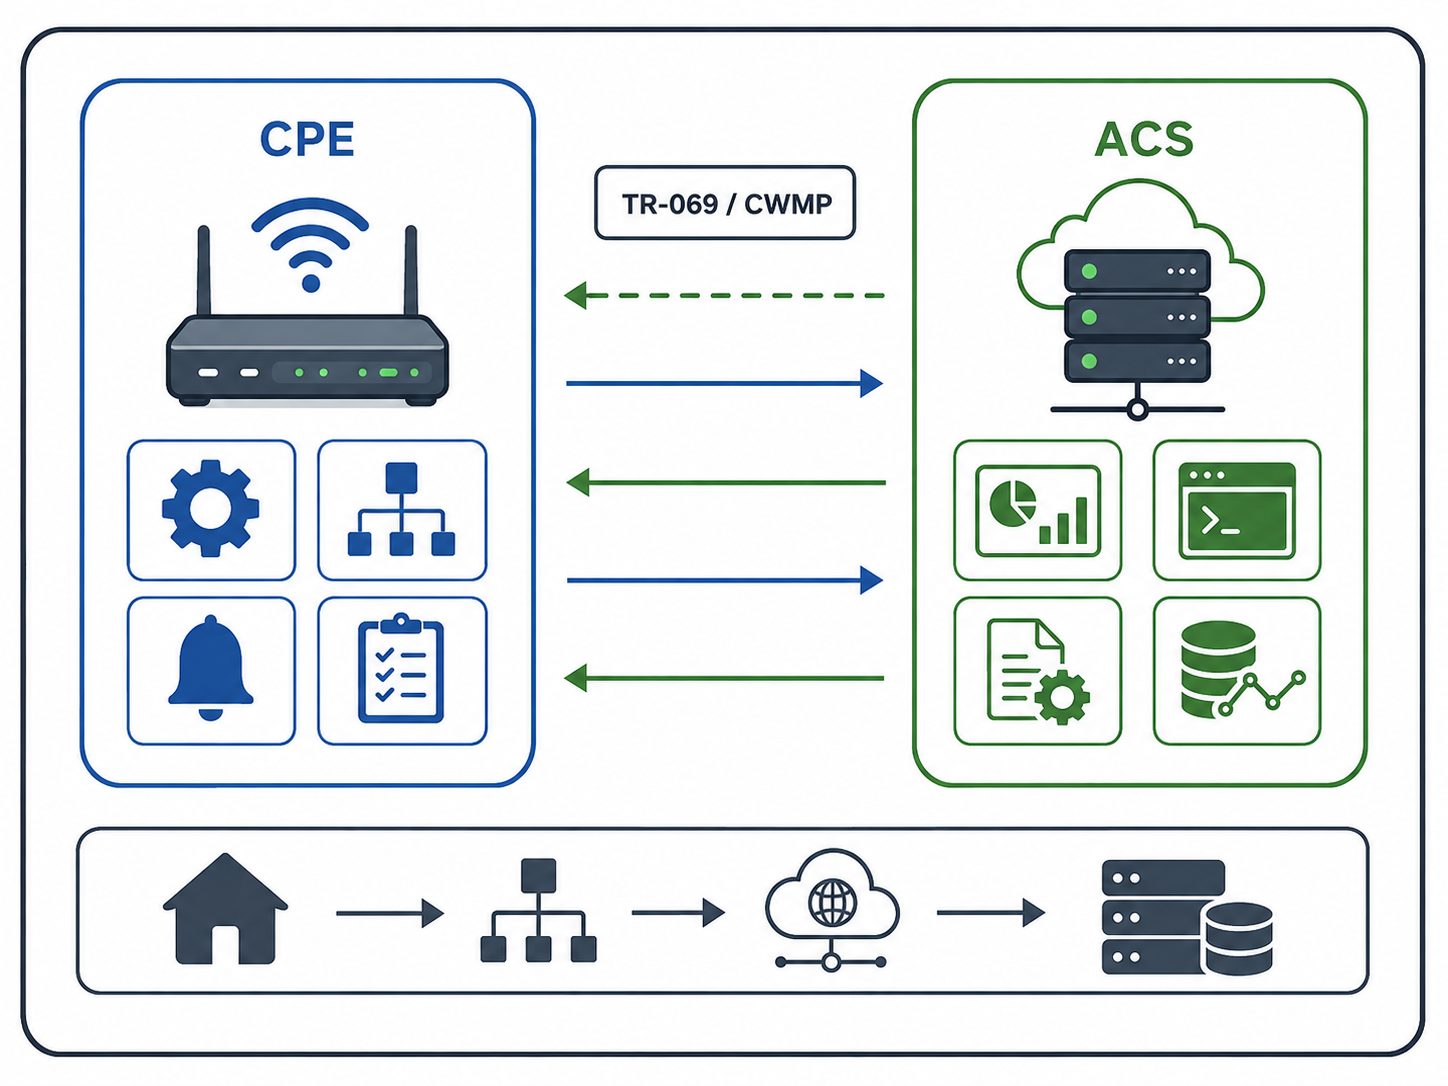
\includegraphics[width=0.88\textwidth]
    {figures/relacion_cpe_acs.png}

    \caption[Relación entre el CPE y el ACS mediante TR-069/CWMP.]
    {Relación entre el CPE y el ACS mediante TR-069/CWMP. El CPE inicia
    normalmente la sesión y comunica su identidad y los eventos mediante
    \texttt{Inform}. El ACS puede solicitar consultas, configuraciones o
    diagnósticos mediante operaciones RPC. Una solicitud de conexión
    permite provocar el establecimiento de una nueva sesión.
    \textit{Fuente: imagen generada mediante ChatGPT (OpenAI) a partir
    de las indicaciones de la autora y basada en la especificación
    TR-069 \cite{bbf_tr069}.}}

    \label{fig:relacion-cpe-acs}
\end{figure}

\subsubsection*{Relación establecida en el laboratorio}

En el laboratorio desarrollado, el TP-Link HX141 principal desempeña la
función de \textbf{CPE gestionado}, mientras que GenieACS actúa como
\textbf{ACS}.

El CPE contiene la configuración necesaria para localizar el servidor y
establece sesiones CWMP con GenieACS. Durante estas sesiones comunica su
identidad y permite que la plataforma consulte las ramas implementadas en
su árbol TR-181.

La relación puede representarse como:

\[
    \text{TP-Link HX141 principal}
    \overset{\text{TR-069/CWMP}}{\longleftrightarrow}
    \text{GenieACS}.
\]

Los agentes EasyMesh secundarios no participan directamente en esta
relación. No disponen de un registro independiente dentro de GenieACS,
sino que su información debe llegar al controlador integrado en el CPE
principal.

Por tanto, existen dos relaciones diferenciadas:

\[
\begin{aligned}
    \text{Controlador}
    &\overset{\text{EasyMesh/IEEE~1905.1}}{\longleftrightarrow}
    \text{Agentes},\\
    \text{CPE principal}
    &\overset{\text{TR-069/CWMP}}{\longleftrightarrow}
    \text{GenieACS}.
\end{aligned}
\]

La primera relación coordina la red mallada dentro del entorno
residencial. La segunda proporciona acceso remoto a la información
expuesta por el dispositivo principal.

GenieACS conserva los valores obtenidos durante las sesiones y permite
consultarlos mediante su interfaz y su API NBI. El exportador utiliza
esta API para acceder a la representación almacenada y convertir los
parámetros seleccionados en métricas de Prometheus.

En consecuencia, la relación entre el CPE y el ACS constituye el
\textbf{enlace entre el entorno residencial y la plataforma de gestión}.
Su correcto funcionamiento resulta imprescindible para trasladar la
telemetría EasyMesh hacia el sistema de observabilidad, aunque la
actualidad de los datos continúa dependiendo de la frecuencia de
actualización del modelo y de las consultas realizadas durante las
sesiones CWMP.

\subsection{Sesiones CWMP}
\label{subsec:sesiones-cwmp}

La comunicación entre el CPE y el ACS se organiza mediante
\textbf{sesiones CWMP}. Una sesión corresponde a un intercambio temporal
de mensajes durante el cual el dispositivo comunica su estado y ambas
entidades ejecutan las operaciones de gestión pendientes
\cite{bbf_tr069}.

A diferencia de otros mecanismos de monitorización, TR-069 no mantiene
necesariamente una conexión permanente entre el dispositivo y la
plataforma. El CPE inicia una sesión cuando se produce un evento que
requiere comunicación con el ACS y la finaliza cuando ambas entidades
dejan de tener mensajes pendientes.

La secuencia general de una sesión puede resumirse mediante las
siguientes etapas:

\begin{enumerate}
    \item el CPE establece una conexión con el ACS;

    \item el CPE envía una llamada \texttt{Inform};

    \item el ACS confirma la recepción mediante
    \texttt{InformResponse};

    \item el ACS envía las solicitudes RPC pendientes;

    \item el CPE ejecuta las operaciones y devuelve sus respuestas;

    \item la sesión finaliza cuando no quedan mensajes por intercambiar.
\end{enumerate}

El flujo simplificado puede representarse como:

\[
\begin{aligned}
    \text{CPE}
    &\xrightarrow{\text{conexión HTTP/HTTPS}}
    \text{ACS}\\
    \text{CPE}
    &\xrightarrow{\texttt{Inform}}
    \text{ACS}\\
    \text{ACS}
    &\xrightarrow{\texttt{InformResponse}}
    \text{CPE}\\
    \text{ACS}
    &\xrightarrow{\text{solicitud RPC}}
    \text{CPE}\\
    \text{CPE}
    &\xrightarrow{\text{respuesta RPC}}
    \text{ACS}.
\end{aligned}
\]


\subsubsection*{Inicio de la sesión}

Las sesiones CWMP son iniciadas normalmente por el
\textbf{CPE}. El dispositivo utiliza la URL configurada en su rama de
gestión para establecer la conexión con el ACS:

\[
    \texttt{Device.ManagementServer.URL}
\]

La conexión utiliza habitualmente HTTP o HTTPS como mecanismo de
transporte. Sobre esta conexión se intercambian mensajes SOAP codificados
mediante XML, dentro de los cuales se incluyen las llamadas y respuestas
RPC definidas por CWMP \cite{bbf_tr069}.

El inicio desde el CPE facilita la gestión de dispositivos situados detrás
de mecanismos de traducción de direcciones o de cortafuegos. El equipo
genera una conexión saliente hacia una dirección previamente configurada,
en lugar de requerir que el ACS mantenga una conexión entrante permanente.

Una sesión puede comenzar como consecuencia de distintos eventos. Entre
los más habituales se encuentran:

\begin{itemize}
    \item la primera conexión del dispositivo con el ACS;
    \item el arranque o reinicio del CPE;
    \item la expiración del intervalo periódico;
    \item la modificación de un parámetro sujeto a notificación;
    \item la finalización de una transferencia;
    \item la terminación de una operación programada;
    \item una solicitud de conexión procedente del ACS.
\end{itemize}

El evento que origina la comunicación se incluye en el mensaje
\texttt{Inform}. El ACS utiliza esta información para determinar el
contexto de la sesión y seleccionar las operaciones que deben ejecutarse.


\subsubsection*{Mensaje inicial \texttt{Inform}}

La primera operación CWMP de una sesión iniciada por el CPE es
habitualmente:

\[
    \texttt{Inform}
\]

Esta llamada permite que el dispositivo comunique:

\begin{itemize}
    \item su identidad;
    \item los eventos que provocan la sesión;
    \item el instante actual del dispositivo;
    \item el número de reintentos realizados;
    \item determinados parámetros de identificación o notificación.
\end{itemize}

La identidad del CPE se representa mediante una estructura que puede
incluir el fabricante, el identificador organizativo, la clase de
producto y el número de serie.

El ACS responde mediante:

\[
    \texttt{InformResponse}
\]

Esta respuesta confirma que el mensaje inicial ha sido recibido y permite
continuar la sesión.

La secuencia inicial es:

\[
\begin{aligned}
    \text{CPE}
    &\xrightarrow{\texttt{Inform}}
    \text{ACS}\\
    \text{ACS}
    &\xrightarrow{\texttt{InformResponse}}
    \text{CPE}.
\end{aligned}
\]

La recepción del \texttt{Inform} no implica que el ACS haya actualizado
automáticamente todo el árbol del dispositivo. El mensaje contiene un
conjunto limitado de información, por lo que la plataforma debe solicitar
posteriormente los objetos y parámetros adicionales que necesite.


\subsubsection*{Eventos asociados a la sesión}

El mensaje \texttt{Inform} incluye uno o varios códigos que indican las
circunstancias que han provocado la comunicación. Algunos eventos
representativos son:

\begin{itemize}
    \item \texttt{0 BOOTSTRAP}, asociado al establecimiento inicial de
    la relación con el ACS o a una modificación relevante de su
    configuración;

    \item \texttt{1 BOOT}, generado después del arranque del
    dispositivo;

    \item \texttt{2 PERIODIC}, generado cuando vence el intervalo de
    comunicación periódica;

    \item \texttt{4 VALUE CHANGE}, relacionado con la modificación de
    parámetros configurados para producir una notificación;

    \item \texttt{6 CONNECTION REQUEST}, generado después de una
    solicitud de conexión procedente del ACS;

    \item \texttt{7 TRANSFER COMPLETE}, relacionado con la finalización
    de una transferencia previamente solicitada.
\end{itemize}

Una misma sesión puede incluir varios eventos. Por ejemplo, después de un
reinicio pueden aparecer simultáneamente códigos asociados al arranque y
a la finalización de una operación anterior.

El ACS no debe interpretar todos los eventos de la misma forma. Una sesión
\texttt{PERIODIC} puede utilizarse para ejecutar consultas rutinarias,
mientras que una sesión \texttt{BOOT} puede requerir comprobar la versión
del firmware, el tiempo de funcionamiento y la configuración aplicada.


\subsubsection*{Comunicación periódica}

TR-069 permite configurar sesiones periódicas mediante los parámetros:

\[
\begin{aligned}
    &\texttt{Device.ManagementServer.PeriodicInformEnable}\\
    &\texttt{Device.ManagementServer.PeriodicInformInterval}\\
    &\texttt{Device.ManagementServer.PeriodicInformTime}
\end{aligned}
\]

Cuando la función se encuentra habilitada, el CPE inicia una sesión cada
vez que vence el intervalo configurado.

La periodicidad puede expresarse como:

\[
    t_n =
    t_{\mathrm{ref}}
    +
    nT_{\mathrm{Inform}},
\]

donde \(t_{\mathrm{ref}}\) representa la referencia temporal,
\(T_{\mathrm{Inform}}\) el intervalo periódico y \(n\) un número entero.

La sesión periódica permite comprobar que el dispositivo mantiene
conectividad con el ACS y proporciona oportunidades recurrentes para
ejecutar operaciones de gestión.

Sin embargo, el establecimiento de una sesión periódica no implica que
todos los parámetros del árbol se consulten nuevamente. La actualización
real depende de las tareas y solicitudes programadas en el ACS.

Por tanto, deben distinguirse:

\[
\begin{aligned}
    T_{\mathrm{sesión}}
    &=
    \text{intervalo entre sesiones CWMP},\\
    T_{\mathrm{consulta}}
    &=
    \text{intervalo entre consultas de un objeto},\\
    T_{\mathrm{modelo}}
    &=
    \text{intervalo de actualización interna del parámetro}.
\end{aligned}
\]

Una sesión puede producirse cada minuto y, aun así, una rama permanecer
desactualizada si el ACS no solicita su contenido o si el firmware no
renueva internamente los valores.


\subsubsection*{Intercambio de operaciones RPC}

Después de confirmar el \texttt{Inform}, el ACS puede enviar
\textbf{operaciones RPC} al CPE. Estas operaciones permiten consultar,
modificar o administrar los elementos expuestos por el dispositivo.

Entre las operaciones disponibles se encuentran:

\begin{itemize}
    \item \texttt{GetParameterValues};
    \item \texttt{SetParameterValues};
    \item \texttt{GetParameterNames};
    \item \texttt{GetParameterAttributes};
    \item \texttt{SetParameterAttributes};
    \item \texttt{AddObject};
    \item \texttt{DeleteObject};
    \item \texttt{Download};
    \item \texttt{Upload};
    \item \texttt{Reboot};
    \item \texttt{FactoryReset}.
\end{itemize}

No todas las operaciones tienen que estar disponibles en todos los
equipos. Su ejecución depende de la versión de CWMP, del modelo de datos,
de las funciones implementadas y de los permisos establecidos por el
firmware.

El intercambio de una operación sigue normalmente el patrón:

\[
\begin{aligned}
    \text{ACS}
    &\xrightarrow{\text{solicitud RPC}}
    \text{CPE}\\
    \text{CPE}
    &\xrightarrow{\text{respuesta RPC}}
    \text{ACS}.
\end{aligned}
\]

Por ejemplo:

\[
\begin{aligned}
    \text{ACS}
    &\xrightarrow{\texttt{GetParameterValues}}
    \text{CPE}\\
    \text{CPE}
    &\xrightarrow{\texttt{GetParameterValuesResponse}}
    \text{ACS}.
\end{aligned}
\]

Las solicitudes y respuestas se procesan dentro de la misma sesión. El
ACS puede encadenar varias operaciones antes de cerrar la comunicación.


\subsubsection*{Procesamiento secuencial}

La sesión CWMP sigue un intercambio ordenado de mensajes. Cada entidad
debe respetar la secuencia del protocolo y responder a las operaciones
recibidas antes de continuar con el resto de las solicitudes.

Este procesamiento secuencial simplifica la asociación entre una
solicitud y su respuesta, pero puede incrementar la duración de la sesión
cuando se consultan numerosos parámetros o ramas extensas.

La duración total puede aproximarse mediante:

\[
    T_{\mathrm{sesión}}
    =
    T_{\mathrm{conexión}}
    +
    T_{\mathrm{Inform}}
    +
    \sum_{i=1}^{N} T_{\mathrm{RPC},i}
    +
    T_{\mathrm{cierre}},
\]

donde \(N\) representa el número de operaciones ejecutadas.

El tiempo de cada operación depende de:

\begin{itemize}
    \item la latencia entre el CPE y el ACS;
    \item el tamaño de la solicitud y de la respuesta;
    \item el número de parámetros consultados;
    \item el tiempo requerido por el firmware para obtener los valores;
    \item la carga del CPE y del ACS.
\end{itemize}

La consulta de un objeto amplio puede generar respuestas de mayor tamaño
y requerir más tiempo que la obtención de un conjunto reducido de
parámetros.


\subsubsection*{Respuestas de error}

Cuando el CPE no puede ejecutar una solicitud, devuelve una
\textbf{respuesta de error o \textit{fault}}. Esta respuesta incluye un
código y una descripción que permiten identificar la causa de la
incidencia \cite{bbf_tr069}.

Una operación puede fallar por motivos como:

\begin{itemize}
    \item la inexistencia del parámetro;
    \item la utilización de una ruta incorrecta;
    \item un tipo de dato incompatible;
    \item la ausencia de permisos de escritura;
    \item un valor situado fuera del rango permitido;
    \item la indisponibilidad temporal de la función;
    \item un error interno del dispositivo.
\end{itemize}

La plataforma debe tratar estos errores de forma explícita. La ausencia
de una respuesta válida no debe interpretarse automáticamente como un
valor igual a cero o como la desactivación de la función.

En una plataforma de monitorización resulta conveniente distinguir entre:

\begin{itemize}
    \item una métrica cuyo valor es cero;
    \item una métrica no implementada;
    \item una consulta fallida;
    \item una métrica sin actualizar;
    \item un CPE sin conectividad con el ACS.
\end{itemize}


\subsubsection*{Finalización de la sesión}

La sesión finaliza cuando el CPE y el ACS dejan de tener mensajes
pendientes. El cierre indica que la comunicación CWMP actual ha
terminado, pero no modifica necesariamente la conectividad ordinaria del
CPE ni el funcionamiento de sus servicios.

Después del cierre, el ACS conserva los valores obtenidos y el CPE
continúa operando hasta que se produce un nuevo evento que requiere otra
sesión.

Por tanto, el funcionamiento general sigue un ciclo discontinuo:

\[
    \text{evento}
    \longrightarrow
    \text{sesión CWMP}
    \longrightarrow
    \text{intercambio de operaciones}
    \longrightarrow
    \text{cierre}
    \longrightarrow
    \text{espera}.
\]

Este comportamiento explica que la información almacenada por el ACS
corresponda a muestras obtenidas en instantes concretos y no a una
transmisión continua del estado del dispositivo.


\subsubsection*{Reintentos de conexión}

El establecimiento de la sesión puede fallar debido a una pérdida de
conectividad, a la indisponibilidad del ACS, a un error de autenticación
o a un problema durante el transporte.

En estos casos, el CPE puede realizar nuevos intentos conforme al
procedimiento de reintento definido por CWMP. El mensaje
\texttt{Inform} incluye un contador que permite comunicar al ACS el número
de intentos efectuados.

La política de reintentos debe evitar que un conjunto elevado de
dispositivos genere conexiones continuas contra una plataforma
indisponible. Para ello, el intervalo entre intentos aumenta conforme se
repiten los fallos y puede incorporar variaciones temporales.

Desde el punto de vista de la observabilidad, los reintentos prolongan la
antigüedad de los parámetros almacenados. Si el CPE no consigue
establecer una sesión, el ACS mantiene los últimos valores conocidos,
aunque el estado real de la red continúe cambiando.


\subsubsection*{Sesiones provocadas por el ACS}

El ACS no abre directamente una sesión CWMP ordinaria contra el CPE. Para
solicitar una comunicación antes del siguiente evento periódico, utiliza
el mecanismo de \textit{Connection Request}.

Después de recibir esta solicitud, el CPE inicia una sesión y comunica el
evento correspondiente mediante \texttt{Inform}:

\[
\begin{aligned}
    \text{ACS}
    &\xrightarrow{\text{\textit{Connection Request}}}
    \text{CPE}\\
    \text{CPE}
    &\xrightarrow{\texttt{Inform}}
    \text{ACS}.
\end{aligned}
\]

Este mecanismo permite reducir el tiempo de espera cuando el operador
necesita consultar o modificar inmediatamente un parámetro.

Sin embargo, su funcionamiento depende de que la dirección de solicitud
sea alcanzable y de que las credenciales se encuentren correctamente
configuradas. En redes con NAT o filtrado de conexiones entrantes puede
no encontrarse disponible de forma directa.


\subsubsection*{Sesiones y actualización de telemetría}

Una sesión CWMP no equivale necesariamente a una actualización completa
de la telemetría. Para que un valor almacenado por el ACS represente el
estado actual deben cumplirse varias condiciones:

\begin{enumerate}
    \item el evento debe ser detectado por el dispositivo;

    \item el firmware debe actualizar el parámetro TR-181;

    \item debe establecerse una sesión CWMP;

    \item el ACS debe solicitar el parámetro o recibirlo mediante una
    notificación;

    \item la plataforma debe almacenar el nuevo valor.
\end{enumerate}

El retardo de adquisición puede expresarse como:

\[
    D_{\mathrm{CWMP}}
    =
    t_{\mathrm{ACS}}
    -
    t_{\mathrm{modelo}},
\]

donde \(t_{\mathrm{modelo}}\) representa el instante en el que el valor se
actualiza en el CPE y \(t_{\mathrm{ACS}}\) el momento en el que queda
almacenado en la plataforma.

Este retardo depende de la periodicidad de las sesiones, de las consultas
programadas y de la duración de cada intercambio.


\subsubsection*{Aplicación en el laboratorio desarrollado}

En el laboratorio del presente proyecto, el TP-Link HX141 principal
establece sesiones CWMP con GenieACS. Durante estas sesiones, el
dispositivo comunica su identidad y permite que la plataforma ejecute
operaciones sobre el árbol TR-181.

La secuencia utilizada puede representarse como:

\[
\begin{aligned}
    \text{TP-Link HX141}
    &\xrightarrow{\texttt{Inform}}
    \text{GenieACS}\\
    \text{GenieACS}
    &\xrightarrow{\text{consulta de parámetros}}
    \text{TP-Link HX141}\\
    \text{TP-Link HX141}
    &\xrightarrow{\text{valores TR-181}}
    \text{GenieACS}.
\end{aligned}
\]

Las sesiones permiten actualizar las ramas relacionadas con la red
Wi-Fi y con la topología EasyMesh. No obstante, la aparición del CPE como
conectado en GenieACS no garantiza que todas estas ramas se hayan
consultado recientemente.

Para mantener una representación actualizada resulta necesario programar
o ejecutar las operaciones de actualización correspondientes. En
GenieACS, estas acciones pueden materializarse mediante tareas que
solicitan la renovación de un objeto concreto.

La plataforma debe conservar al menos:

\begin{itemize}
    \item el instante de la última sesión;
    \item el último evento comunicado;
    \item el estado de las tareas ejecutadas;
    \item el instante de actualización de los parámetros;
    \item los errores producidos durante las consultas.
\end{itemize}

Esta información permite diferenciar una pérdida de conectividad CWMP de
una ausencia real de clientes o agentes en la red EasyMesh.

En consecuencia, las sesiones CWMP constituyen el
\textbf{marco temporal y operativo dentro del cual el CPE y el ACS
intercambian información}. Su frecuencia y contenido determinan la
actualidad de la representación almacenada en GenieACS y condicionan el
retardo con el que la plataforma de observabilidad detecta los cambios
producidos en la red mallada.

\subsection{Inform, GetParameterValues y refreshObject}
\label{subsec:inform-getparametervalues-refreshobject}

La actualización de los parámetros almacenados en el ACS requiere
diferenciar tres operaciones relacionadas, pero pertenecientes a niveles
distintos de la arquitectura: \texttt{Inform},
\texttt{GetParameterValues} y \texttt{refreshObject}.

Las operaciones \texttt{Inform} y \texttt{GetParameterValues} forman
parte del protocolo \textbf{TR-069/CWMP}. En cambio,
\texttt{refreshObject} no es una llamada RPC definida por TR-069, sino
una \textbf{tarea interna de GenieACS} utilizada para solicitar la
actualización de un objeto del modelo de datos
\cite{bbf_tr069,genieacs_api}.

La relación general entre las tres operaciones puede resumirse mediante:

\[
\begin{aligned}
    \text{CPE}
    &\xrightarrow{\texttt{Inform}}
    \text{GenieACS}\\
    \text{GenieACS}
    &\xrightarrow{\texttt{GetParameterValues}}
    \text{CPE}\\
    \text{Operador o aplicación}
    &\xrightarrow{\texttt{refreshObject}}
    \text{GenieACS}.
\end{aligned}
\]

El mensaje \texttt{Inform} permite establecer la sesión y comunicar
eventos. La llamada \texttt{GetParameterValues} obtiene valores concretos
del dispositivo. La tarea \texttt{refreshObject} indica a GenieACS qué
rama debe actualizar mediante las operaciones CWMP necesarias.


\subsubsection*{Operación \texttt{Inform}}

La llamada:

\[
    \texttt{Inform}
\]

es enviada por el CPE al ACS al comienzo de una sesión CWMP. Su finalidad
consiste en identificar al dispositivo, comunicar los eventos que
originan la sesión y proporcionar un conjunto inicial de parámetros
\cite{bbf_tr069}.

El contenido de la llamada incluye estructuras como:

\begin{itemize}
    \item \texttt{DeviceId};
    \item \texttt{Event};
    \item \texttt{MaxEnvelopes};
    \item \texttt{CurrentTime};
    \item \texttt{RetryCount};
    \item \texttt{ParameterList}.
\end{itemize}

La estructura \texttt{DeviceId} contiene los datos utilizados para
identificar al equipo, como el fabricante, el identificador organizativo,
la clase de producto y el número de serie.

La estructura \texttt{Event} contiene uno o varios códigos que explican
por qué el dispositivo ha establecido la sesión. Entre los eventos más
habituales se encuentran:

\begin{itemize}
    \item \texttt{0 BOOTSTRAP};
    \item \texttt{1 BOOT};
    \item \texttt{2 PERIODIC};
    \item \texttt{4 VALUE CHANGE};
    \item \texttt{6 CONNECTION REQUEST};
    \item \texttt{7 TRANSFER COMPLETE}.
\end{itemize}

El campo \texttt{ParameterList} contiene determinados parámetros que el
CPE debe comunicar o que se encuentran configurados para generar
notificaciones.

Sin embargo, el mensaje \texttt{Inform} no contiene necesariamente todos
los objetos y parámetros implementados por el dispositivo. Su recepción
tampoco provoca por sí sola la actualización completa del árbol
almacenado en GenieACS.

La secuencia inicial de la sesión es:

\[
\begin{aligned}
    \text{CPE}
    &\xrightarrow{\texttt{Inform}}
    \text{ACS}\\
    \text{ACS}
    &\xrightarrow{\texttt{InformResponse}}
    \text{CPE}.
\end{aligned}
\]

La respuesta \texttt{InformResponse} confirma que el ACS ha procesado el
mensaje inicial. A continuación, GenieACS puede enviar las operaciones
RPC necesarias para ejecutar las tareas pendientes.

Por tanto, debe diferenciarse entre:

\begin{itemize}
    \item la \textbf{recepción de un \texttt{Inform}}, que confirma la
    comunicación del CPE y comunica determinados eventos;

    \item la \textbf{actualización de parámetros}, que requiere que el
    ACS solicite sus valores o que estos se incluyan en el propio
    mensaje.
\end{itemize}

Un dispositivo puede aparecer recientemente conectado en GenieACS porque
ha enviado un \texttt{Inform}, mientras que algunas ramas de su modelo de
datos conservan valores obtenidos durante sesiones anteriores.


\subsubsection*{Operación \texttt{GetParameterValues}}

La llamada:

\[
    \texttt{GetParameterValues}
\]

es una operación RPC enviada por el ACS para solicitar al CPE los valores
de uno o varios parámetros de su modelo de datos
\cite{bbf_tr069}.

La solicitud contiene una lista denominada \texttt{ParameterNames}. Esta
lista puede incluir rutas correspondientes a parámetros concretos o rutas
parciales pertenecientes a un objeto.

Un ejemplo de consulta de un parámetro individual es:

\[
    \texttt{Device.DeviceInfo.SoftwareVersion}
\]

Otro ejemplo aplicado a la red Wi-Fi es:

\[
    \texttt{Device.WiFi.Radio.1.Channel}
\]

El intercambio puede representarse como:

\[
\begin{aligned}
    \text{ACS}
    &\xrightarrow{\texttt{GetParameterValues}}
    \text{CPE}\\
    \text{CPE}
    &\xrightarrow{\texttt{GetParameterValuesResponse}}
    \text{ACS}.
\end{aligned}
\]

La respuesta contiene una lista de parámetros con:

\begin{itemize}
    \item la ruta completa;
    \item el valor actual;
    \item el tipo de dato correspondiente.
\end{itemize}

De forma conceptual, una respuesta puede contener:

\begin{verbatim}
Device.WiFi.Radio.1.Channel = 36
Device.WiFi.Radio.1.Status = "Up"
Device.WiFi.Radio.1.OperatingFrequencyBand = "5GHz"
\end{verbatim}

El ACS utiliza esta respuesta para actualizar los valores almacenados en
su base de datos.

Cuando se solicita una ruta parcial, el CPE puede devolver los parámetros
incluidos bajo dicha rama. Por ejemplo, una consulta sobre:

\[
    \texttt{Device.WiFi.Radio.1.}
\]

puede recuperar los parámetros legibles pertenecientes a la primera
instancia de la tabla de radios.

La consulta de una rama extensa puede generar una respuesta de gran
tamaño. Dependiendo de la capacidad del dispositivo y del servidor, puede
ser necesario dividir la adquisición en varias operaciones.

La duración de la consulta depende de:

\begin{itemize}
    \item el número de parámetros solicitados;
    \item el tamaño de los valores;
    \item la latencia entre el CPE y el ACS;
    \item la capacidad de procesamiento del dispositivo;
    \item el tiempo necesario para obtener los valores internos;
    \item los límites de tamaño admitidos por la implementación.
\end{itemize}

Si el CPE no reconoce una ruta o no puede procesar la solicitud, devuelve
una respuesta de error. Esta situación debe diferenciarse de un parámetro
que existe y cuyo valor es igual a cero.

Para una plataforma de monitorización, deben distinguirse al menos los
siguientes estados:

\begin{itemize}
    \item parámetro obtenido correctamente;
    \item parámetro con valor cero;
    \item parámetro no implementado;
    \item ruta desconocida;
    \item consulta fallida;
    \item valor almacenado sin actualizar.
\end{itemize}


\subsubsection*{Descubrimiento y consulta de parámetros}

Para obtener valores de un objeto, el ACS debe conocer previamente las
rutas implementadas por el dispositivo. Esta información puede
descubrirse mediante la llamada:

\[
    \texttt{GetParameterNames}
\]

Esta operación permite consultar los nombres de los objetos y parámetros
disponibles bajo una ruta determinada.

Por tanto, el proceso de actualización de una rama puede requerir dos
tipos de operaciones:

\begin{enumerate}
    \item descubrir los objetos, instancias y parámetros existentes;

    \item solicitar los valores de los parámetros descubiertos.
\end{enumerate}

La secuencia conceptual es:

\[
\begin{aligned}
    \text{ACS}
    &\xrightarrow{\texttt{GetParameterNames}}
    \text{CPE}\\
    \text{CPE}
    &\xrightarrow{\text{nombres disponibles}}
    \text{ACS}\\
    \text{ACS}
    &\xrightarrow{\texttt{GetParameterValues}}
    \text{CPE}\\
    \text{CPE}
    &\xrightarrow{\text{valores}}
    \text{ACS}.
\end{aligned}
\]

Esta fase resulta especialmente importante en tablas dinámicas, como las
que representan clientes asociados. La aparición o desaparición de una
estación puede modificar el número y la posición de las instancias
existentes.

Consultar únicamente los valores de las instancias almacenadas
previamente puede impedir detectar nuevas entradas. Por ello, la
actualización debe considerar tanto la estructura de la tabla como los
valores de sus parámetros.


\subsubsection*{Tarea \texttt{refreshObject} de GenieACS}

La operación:

\[
    \texttt{refreshObject}
\]

es una \textbf{tarea propia de GenieACS}. No forma parte del conjunto de
llamadas RPC definido por TR-069/CWMP
\cite{genieacs_api}.

Su finalidad consiste en indicar a GenieACS que debe renovar la
información almacenada bajo un objeto determinado. La tarea puede
generarse desde la interfaz de GenieACS o mediante su API NBI.

Una tarea presenta una estructura similar a:

\begin{verbatim}
{
    "name": "refreshObject",
    "objectName": "Device.WiFi.DataElements."
}
\end{verbatim}

El campo \texttt{name} identifica el tipo de tarea y
\texttt{objectName} especifica la rama que debe actualizarse.

GenieACS procesa esta instrucción y determina las operaciones CWMP
necesarias para sincronizar el objeto con el dispositivo. Dependiendo de
la información almacenada y de la estructura de la rama, la actualización
puede requerir descubrir objetos e instancias y solicitar posteriormente
sus valores.

Por tanto, no debe representarse la comunicación como:

\[
    \text{ACS}
    \xrightarrow{\texttt{refreshObject}}
    \text{CPE},
\]

porque el CPE no recibe una llamada RPC denominada
\texttt{refreshObject}.

La representación correcta es:

\[
\begin{aligned}
    \text{Operador o aplicación}
    &\xrightarrow{\texttt{refreshObject}}
    \text{GenieACS}\\
    \text{GenieACS}
    &\xrightarrow{\text{operaciones CWMP}}
    \text{CPE}\\
    \text{CPE}
    &\xrightarrow{\text{respuestas CWMP}}
    \text{GenieACS}.
\end{aligned}
\]

Entre las operaciones CWMP utilizadas por GenieACS pueden encontrarse
consultas de nombres y valores, según el estado del modelo almacenado y
las características del objeto solicitado.


\subsubsection*{Ejecución inmediata o diferida}

Cuando se crea una tarea \texttt{refreshObject}, esta puede quedar
almacenada hasta la siguiente sesión iniciada por el CPE.

La API de GenieACS permite solicitar además una
\textbf{\textit{Connection Request}} para intentar provocar que el
dispositivo establezca inmediatamente una nueva sesión
\cite{genieacs_api}.

Sin solicitud de conexión, la secuencia es:

\[
\begin{aligned}
    \text{Aplicación}
    &\xrightarrow{\text{crear tarea}}
    \text{GenieACS}\\
    \text{CPE}
    &\xrightarrow{\text{siguiente \texttt{Inform}}}
    \text{GenieACS}\\
    \text{GenieACS}
    &\xrightarrow{\text{ejecución de la tarea}}
    \text{CPE}.
\end{aligned}
\]

Cuando se solicita una conexión inmediata, la secuencia conceptual es:

\[
\begin{aligned}
    \text{GenieACS}
    &\xrightarrow{\text{\textit{Connection Request}}}
    \text{CPE}\\
    \text{CPE}
    &\xrightarrow{\texttt{Inform}}
    \text{GenieACS}\\
    \text{GenieACS}
    &\xrightarrow{\text{operaciones de actualización}}
    \text{CPE}.
\end{aligned}
\]

La ejecución inmediata depende de que el mecanismo de
\textit{Connection Request} sea alcanzable y se encuentre correctamente
configurado. Cuando no puede utilizarse, la tarea permanece pendiente
hasta que el CPE inicia una nueva sesión.


\subsubsection*{Actualización completa o selectiva}

La tarea puede aplicarse a una rama concreta:

\begin{verbatim}
{
    "name": "refreshObject",
    "objectName": "Device.WiFi.DataElements."
}
\end{verbatim}

También puede solicitarse la actualización de una subrama más reducida:

\begin{verbatim}
{
    "name": "refreshObject",
    "objectName":
    "Device.WiFi.DataElements.Network.Device.1.Radio.1."
}
\end{verbatim}

La selección de una rama concreta reduce el número de parámetros que
deben consultarse y disminuye la carga sobre el dispositivo, la red y el
ACS.

La API también permite solicitar una actualización general utilizando un
nombre de objeto vacío. No obstante, actualizar periódicamente todo el
modelo puede resultar costoso cuando el árbol contiene numerosas
instancias y parámetros.

Por este motivo, una estrategia de monitorización debe priorizar las
ramas necesarias para los objetivos del proyecto:

\begin{itemize}
    \item dispositivos EasyMesh;
    \item radios;
    \item BSS;
    \item estaciones asociadas;
    \item métricas del cliente seleccionado;
    \item marcas temporales relevantes.
\end{itemize}

La actualización selectiva evita consultar de forma reiterada parámetros
de configuración que permanecen estables y no intervienen en el análisis.


\subsubsection*{Base de datos de GenieACS y estado del CPE}

GenieACS conserva en su base de datos una representación de los objetos y
parámetros obtenidos del dispositivo. La consulta de esta base de datos
mediante la API NBI no provoca automáticamente una nueva comunicación con
el CPE \cite{genieacs_api}.

Por tanto, una consulta realizada por el exportador sigue la secuencia:

\[
    \text{Exportador}
    \xrightarrow{\text{consulta NBI}}
    \text{base de datos de GenieACS}.
\]

No debe interpretarse como:

\[
    \text{Exportador}
    \longrightarrow
    \text{GenieACS}
    \longrightarrow
    \text{consulta inmediata al CPE}.
\]

La API devuelve los valores que GenieACS tiene almacenados en ese
momento. La actualidad de dichos valores depende de que se haya ejecutado
previamente una tarea de actualización o una consulta equivalente durante
una sesión CWMP.

Deben diferenciarse, por tanto:

\begin{itemize}
    \item el \textbf{estado actual de la red EasyMesh};
    \item el \textbf{valor actual dentro del CPE};
    \item el \textbf{valor obtenido durante la última sesión CWMP};
    \item el \textbf{valor almacenado en GenieACS};
    \item el \textbf{valor leído por el exportador mediante la API NBI}.
\end{itemize}

Esta distinción resulta esencial para interpretar correctamente la
telemetría.


\subsubsection*{Secuencia completa de actualización}

La actualización de una rama puede representarse mediante la siguiente
secuencia:

\[
\begin{aligned}
    \text{Aplicación}
    &\xrightarrow{\texttt{refreshObject}}
    \text{GenieACS}\\
    \text{GenieACS}
    &\xrightarrow{\text{tarea pendiente}}
    \text{cola de tareas}\\
    \text{CPE}
    &\xrightarrow{\texttt{Inform}}
    \text{GenieACS}\\
    \text{GenieACS}
    &\xrightarrow{\text{RPC de consulta}}
    \text{CPE}\\
    \text{CPE}
    &\xrightarrow{\text{valores}}
    \text{GenieACS}\\
    \text{GenieACS}
    &\xrightarrow{\text{actualización}}
    \text{base de datos}.
\end{aligned}
\]

Una vez completado el proceso, el exportador puede consultar los nuevos
valores:

\[
\begin{aligned}
    \text{Exportador}
    &\xrightarrow{\text{API NBI}}
    \text{GenieACS}\\
    \text{GenieACS}
    &\xrightarrow{\text{datos almacenados}}
    \text{Exportador}.
\end{aligned}
\]

Finalmente, el exportador transforma los parámetros en métricas y los
expone para que Prometheus los recopile.


\subsubsection*{Actualización de tablas dinámicas}

Las tablas de clientes asociados presentan una estructura dinámica. Un
cliente puede conectarse, desconectarse o cambiar de BSS, provocando la
aparición o desaparición de instancias.

En estas tablas no basta con actualizar únicamente el valor de parámetros
conocidos. También debe renovarse la estructura para descubrir:

\begin{itemize}
    \item nuevas instancias;
    \item instancias eliminadas;
    \item cambios en la posición del cliente;
    \item modificaciones en la relación entre STA, BSS, radio y
    dispositivo.
\end{itemize}

En el caso de \texttt{Device.WiFi.DataElements.}, una actualización debe
permitir comprobar la jerarquía:

\[
    \texttt{Network.Device.Radio.BSS.STA}.
\]

Después de un cambio de asociación, la dirección MAC del cliente puede
desaparecer de una instancia y aparecer bajo otro BSS. Si GenieACS no
renueva la estructura, puede conservar temporalmente la posición
anterior.

Por tanto, la tarea de actualización debe abarcar el nivel necesario para
redescubrir las instancias relacionadas con el cliente.


\subsubsection*{Periodicidad y carga de las consultas}

La ejecución frecuente de \texttt{refreshObject} mejora la actualidad de
los datos, pero aumenta la carga sobre:

\begin{itemize}
    \item el cliente CWMP del CPE;
    \item la conectividad entre el CPE y el ACS;
    \item el servicio CWMP de GenieACS;
    \item la base de datos;
    \item la cola de tareas.
\end{itemize}

La periodicidad debe seleccionarse equilibrando la
\textbf{actualidad de la telemetría} y el
\textbf{coste de adquisición}.

Si \(T_r\) representa el intervalo entre actualizaciones, una reducción
de \(T_r\) permite detectar los cambios con menor retardo, pero incrementa
el número de sesiones y operaciones ejecutadas.

Además, la frecuencia de consulta no debe ser inferior de forma
significativa a la frecuencia con la que el firmware actualiza
internamente los parámetros. De lo contrario, varias consultas
consecutivas pueden devolver el mismo valor.

Deben considerarse al menos tres intervalos:

\[
\begin{aligned}
    T_{\mathrm{interno}}
    &=
    \text{actualización del parámetro en el CPE},\\
    T_{\mathrm{refresh}}
    &=
    \text{ejecución de \texttt{refreshObject}},\\
    T_{\mathrm{scrape}}
    &=
    \text{adquisición realizada por Prometheus}.
\end{aligned}
\]

La configuración debe evitar que Prometheus consulte el exportador con
una frecuencia elevada mientras GenieACS conserva valores que no han sido
renovados.


\subsubsection*{Aplicación en el laboratorio desarrollado}

En el laboratorio, el TP-Link HX141 principal envía mensajes
\texttt{Inform} a GenieACS para establecer las sesiones CWMP. Durante
estas sesiones, GenieACS puede ejecutar las tareas pendientes y obtener
los parámetros solicitados.

La tarea \texttt{refreshObject} se utiliza para renovar las ramas
relacionadas con la topología y la telemetría EasyMesh, especialmente:

\[
    \texttt{Device.WiFi.DataElements.}
\]

El flujo utilizado puede resumirse como:

\[
\begin{aligned}
    \text{TP-Link HX141}
    &\xrightarrow{\texttt{Inform}}
    \text{GenieACS}\\
    \text{GenieACS}
    &\xrightarrow{\text{consultas CWMP}}
    \text{TP-Link HX141}\\
    \text{TP-Link HX141}
    &\xrightarrow{\text{valores TR-181}}
    \text{GenieACS}\\
    \text{Exportador}
    &\xrightarrow{\text{API NBI}}
    \text{GenieACS}.
\end{aligned}
\]

El exportador no utiliza \texttt{GetParameterValues} directamente contra
el CPE. Su fuente de datos es la representación almacenada por GenieACS.

Por esta razón, la plataforma debe comprobar:

\begin{itemize}
    \item el instante de la última sesión CWMP;
    \item el estado de la tarea \texttt{refreshObject};
    \item el instante de actualización de la rama;
    \item la existencia de errores de consulta;
    \item la antigüedad de los valores obtenidos mediante la API NBI.
\end{itemize}

Una métrica ausente no debe interpretarse automáticamente como la
desaparición del cliente. Puede deberse a que la tarea permanece
pendiente, la sesión no se ha establecido, la consulta ha fallado o la
rama no se ha actualizado correctamente.

En consecuencia, las tres operaciones desempeñan funciones
complementarias:

\begin{itemize}
    \item \texttt{Inform} establece la sesión y comunica los eventos del
    CPE;

    \item \texttt{GetParameterValues} obtiene los valores de los
    parámetros solicitados;

    \item \texttt{refreshObject} indica a GenieACS qué objeto debe
    sincronizar con el dispositivo.
\end{itemize}

La correcta coordinación de estas operaciones determina la actualidad de
la información almacenada en GenieACS y, por extensión, el retardo con el
que Prometheus y Grafana muestran los cambios producidos en la red
EasyMesh.

\subsection{Función de GenieACS como ACS}
\label{subsec:funcion-genieacs-acs}

\textbf{GenieACS} es una plataforma de gestión que implementa las
funciones de un \textbf{ACS} para dispositivos compatibles con
TR-069/CWMP. Su finalidad consiste en recibir las sesiones iniciadas por
los CPE, ejecutar operaciones de gestión remota y mantener una
representación de los objetos y parámetros obtenidos de cada dispositivo
\cite{genieacs_documentation,bbf_tr069}.

Dentro de la arquitectura desarrollada, GenieACS constituye el punto de
unión entre el CPE TP-Link HX141 y el sistema de observabilidad. La
plataforma recibe la información expuesta mediante TR-181, la almacena y
permite que otras aplicaciones accedan a ella mediante su interfaz
\textbf{NBI} (\textit{Northbound Interface}).

Su función general puede representarse como:

\[
\begin{aligned}
    \text{CPE}
    &\overset{\text{TR-069/CWMP}}{\longleftrightarrow}
    \text{GenieACS}\\
    \text{Aplicaciones externas}
    &\overset{\text{API NBI}}{\longleftrightarrow}
    \text{GenieACS}.
\end{aligned}
\]

GenieACS no participa directamente en la comunicación interna entre el
controlador y los agentes EasyMesh. Su ámbito comienza cuando el CPE
principal establece una sesión CWMP y proporciona acceso a los objetos y
parámetros de su modelo de datos.

Por tanto, deben diferenciarse dos planos de comunicación:

\[
\begin{aligned}
    \text{Controlador EasyMesh}
    &\overset{\text{EasyMesh/IEEE~1905.1}}{\longleftrightarrow}
    \text{Agentes},\\
    \text{CPE principal}
    &\overset{\text{TR-069/CWMP}}{\longleftrightarrow}
    \text{GenieACS}.
\end{aligned}
\]

El primer intercambio se produce dentro de la red residencial y permite
coordinar la infraestructura Multi-AP. El segundo permite trasladar hacia
la plataforma de gestión la información que el firmware incorpora al
modelo TR-181.


\subsubsection*{Componentes principales de GenieACS}

GenieACS se organiza mediante varios servicios independientes, cada uno
destinado a una función concreta. Los componentes principales son
\cite{genieacs_documentation}:

\begin{itemize}
    \item \texttt{genieacs-cwmp};
    \item \texttt{genieacs-nbi};
    \item \texttt{genieacs-fs};
    \item \texttt{genieacs-ui}.
\end{itemize}

La Tabla~\ref{tab:componentes-genieacs} resume la función de estos
servicios.

\begin{table}[H]
    \centering
    \small
    \renewcommand{\arraystretch}{1.35}

    \caption[Componentes principales de GenieACS.]
    {Componentes principales de GenieACS y función desempeñada dentro de
    la plataforma.
    \textit{Fuente: elaboración propia a partir de la documentación de
    GenieACS \cite{genieacs_documentation}.}}

    \label{tab:componentes-genieacs}

    \begin{tabular}{
        p{0.28\textwidth}
        p{0.62\textwidth}
    }
        \hline
        \textbf{Componente}
        &
        \textbf{Función}
        \\
        \hline

        \texttt{genieacs-cwmp}
        &
        Recibe las conexiones TR-069, procesa los mensajes
        \texttt{Inform} y gestiona las operaciones RPC intercambiadas con
        los CPE.
        \\

        \texttt{genieacs-nbi}
        &
        Proporciona una API REST para consultar dispositivos, tareas,
        configuraciones y otros elementos almacenados por GenieACS.
        \\

        \texttt{genieacs-fs}
        &
        Proporciona el servicio de archivos utilizado en operaciones como
        la descarga de firmware o de configuraciones hacia los CPE.
        \\

        \texttt{genieacs-ui}
        &
        Ofrece la interfaz web utilizada para consultar dispositivos,
        revisar parámetros, crear tareas y administrar la plataforma.
        \\

        \hline
    \end{tabular}
\end{table}

Los servicios pueden ejecutarse en un mismo sistema o distribuirse entre
varios servidores. Esta separación permite adaptar el despliegue a las
necesidades de capacidad, disponibilidad y escalabilidad de la
plataforma \cite{genieacs_documentation}.


\subsubsection*{Servicio \texttt{genieacs-cwmp}}

El componente:

\[
    \texttt{genieacs-cwmp}
\]

implementa la interfaz utilizada para recibir y procesar las
\textbf{sesiones TR-069/CWMP}. El CPE se conecta a este servicio mediante
la URL configurada en:

\[
    \texttt{Device.ManagementServer.URL}
\]

Cuando el dispositivo inicia una sesión, el servicio recibe el mensaje
\texttt{Inform}, identifica el CPE y determina las operaciones que deben
ejecutarse.

Entre sus responsabilidades se encuentran:

\begin{itemize}
    \item recibir las conexiones de los CPE;
    \item procesar los mensajes SOAP y XML;
    \item identificar los eventos de la sesión;
    \item ejecutar las tareas pendientes;
    \item enviar solicitudes RPC;
    \item procesar las respuestas del dispositivo;
    \item registrar errores y resultados;
    \item actualizar la representación almacenada del modelo de datos.
\end{itemize}

El componente CWMP no consulta de manera continua al dispositivo. Las
operaciones se ejecutan dentro de las sesiones iniciadas por el CPE o
provocadas mediante una solicitud de conexión.

La secuencia general es:

\[
\begin{aligned}
    \text{CPE}
    &\xrightarrow{\texttt{Inform}}
    \texttt{genieacs-cwmp}\\
    \texttt{genieacs-cwmp}
    &\xrightarrow{\text{solicitud RPC}}
    \text{CPE}\\
    \text{CPE}
    &\xrightarrow{\text{respuesta RPC}}
    \texttt{genieacs-cwmp}.
\end{aligned}
\]

Cuando una tarea \texttt{refreshObject} se encuentra pendiente, este
servicio ejecuta las operaciones CWMP necesarias para descubrir y
actualizar el objeto solicitado.


\subsubsection*{Persistencia de la información}

GenieACS utiliza una base de datos para conservar la información
relacionada con los dispositivos, los parámetros, las tareas, las
configuraciones y otros elementos de la plataforma.

La información almacenada sobre un dispositivo incluye:

\begin{itemize}
    \item su identificador;
    \item los parámetros descubiertos;
    \item los valores obtenidos;
    \item los tipos de datos;
    \item las marcas temporales de actualización;
    \item las tareas pendientes;
    \item las etiquetas asignadas;
    \item determinados datos relacionados con las sesiones.
\end{itemize}

Esta representación constituye una \textbf{copia persistente del último
estado conocido} por GenieACS. No debe confundirse con una consulta en
tiempo real del dispositivo.

El flujo de actualización puede expresarse como:

\[
\begin{aligned}
    \text{CPE}
    &\xrightarrow{\text{respuesta CWMP}}
    \text{GenieACS}\\
    \text{GenieACS}
    &\xrightarrow{\text{almacenamiento}}
    \text{base de datos}.
\end{aligned}
\]

Posteriormente, la interfaz web y la API NBI consultan esta representación
almacenada.

Por tanto, una lectura realizada mediante la API sigue la secuencia:

\[
    \text{Aplicación}
    \xrightarrow{\text{consulta NBI}}
    \text{base de datos de GenieACS}.
\]

La consulta NBI no provoca automáticamente una nueva operación
\texttt{GetParameterValues} contra el CPE. Para obtener información
actualizada debe haberse ejecutado previamente una tarea o una
declaración que fuerce la sincronización con el dispositivo
\cite{genieacs_api}.


\subsubsection*{Descubrimiento del modelo de datos}

GenieACS mantiene una representación de las rutas implementadas por cada
CPE. Sin embargo, por motivos de rendimiento, no obtiene necesariamente
todo el árbol del dispositivo en cada sesión.

La plataforma descubre y actualiza los objetos necesarios para satisfacer
las tareas, provisiones y consultas configuradas. Cuando se necesita
explorar una rama adicional puede solicitarse su actualización desde la
interfaz web o mediante una tarea \texttt{refreshObject}
\cite{genieacs_documentation,genieacs_api}.

Esta característica resulta importante porque la ausencia de una ruta en
la interfaz de GenieACS puede tener varios significados:

\begin{itemize}
    \item el dispositivo no implementa el objeto;
    \item GenieACS todavía no ha descubierto la ruta;
    \item la rama no se ha actualizado después de una reconfiguración;
    \item la consulta anterior ha producido un error;
    \item el objeto ha desaparecido del modelo del CPE.
\end{itemize}

Por tanto, antes de concluir que una métrica no se encuentra disponible,
debe comprobarse si el objeto correspondiente ha sido descubierto y
actualizado correctamente.

Esta consideración resulta especialmente relevante para las tablas
dinámicas de clientes:

\[
    \texttt{Device.WiFi.DataElements.Network.Device.Radio.BSS.STA}
\]

La estructura de estas tablas puede cambiar cuando un cliente se conecta,
se desconecta o modifica su punto de asociación. GenieACS debe redescubrir
las instancias para reflejar correctamente la nueva organización.


\subsubsection*{Tareas de gestión}

GenieACS permite crear \textbf{tareas} asociadas a un dispositivo. Estas
tareas representan operaciones que deben ejecutarse durante una sesión
CWMP.

Entre las tareas disponibles se encuentran acciones destinadas a:

\begin{itemize}
    \item actualizar un objeto;
    \item establecer valores de parámetros;
    \item reiniciar el dispositivo;
    \item restaurar su configuración;
    \item descargar archivos;
    \item añadir o eliminar instancias.
\end{itemize}

Una tarea puede permanecer pendiente hasta que el CPE establece una nueva
sesión. Cuando resulta necesario reducir el tiempo de espera, GenieACS
puede intentar enviar una solicitud de conexión para provocar que el
dispositivo contacte con el ACS.

En el contexto de la monitorización, la tarea principal es:

\[
    \texttt{refreshObject}
\]

Esta tarea indica a GenieACS que debe renovar una rama determinada. Por
ejemplo:

\begin{verbatim}
{
    "name": "refreshObject",
    "objectName": "Device.WiFi.DataElements."
}
\end{verbatim}

La creación de la tarea no garantiza su ejecución inmediata. El resultado
depende de:

\begin{itemize}
    \item la disponibilidad del CPE;
    \item el establecimiento de una sesión CWMP;
    \item el funcionamiento de la solicitud de conexión;
    \item la existencia del objeto;
    \item la capacidad del dispositivo para responder;
    \item la ausencia de errores durante la consulta.
\end{itemize}

Por este motivo, la aplicación que crea una tarea debe comprobar
posteriormente su estado y verificar que los parámetros presentan una
marca temporal reciente.


\subsubsection*{Provisiones y reglas automáticas}

GenieACS permite definir \textbf{provisiones}, que consisten en programas
ejecutados en el servidor para aplicar lógica de configuración y
sincronización sobre los dispositivos.

Las provisiones pueden utilizarse para:

\begin{itemize}
    \item declarar parámetros que deben mantenerse actualizados;
    \item aplicar configuraciones;
    \item comprobar valores;
    \item crear o eliminar instancias;
    \item ejecutar acciones según el modelo del CPE;
    \item invocar extensiones externas.
\end{itemize}

La función \texttt{declare} permite especificar los parámetros necesarios
y establecer restricciones sobre la antigüedad aceptada para sus valores.
Cuando el dato almacenado no cumple la condición temporal, GenieACS
solicita su actualización durante la sesión
\cite{genieacs_documentation}.

De forma conceptual:

\[
    \text{valor almacenado antiguo}
    \longrightarrow
    \text{declaración de actualización}
    \longrightarrow
    \text{consulta al CPE}.
\]

Las provisiones pueden asociarse a los dispositivos mediante
\textbf{presets}. Un preset determina bajo qué condiciones debe ejecutarse
una provisión, por ejemplo según el fabricante, el modelo, una etiqueta o
un evento recibido.

Estas funciones permiten automatizar la gestión de un conjunto elevado de
CPE. No obstante, las provisiones deben diseñarse de manera controlada
para evitar consultas innecesarias o modificaciones repetidas sobre el
dispositivo.


\subsubsection*{Interfaz de administración}

El componente:

\[
    \texttt{genieacs-ui}
\]

proporciona la interfaz web de administración. Desde ella pueden
consultarse los dispositivos registrados y examinarse los objetos y
parámetros almacenados.

La interfaz permite realizar tareas como:

\begin{itemize}
    \item buscar y seleccionar dispositivos;
    \item consultar parámetros;
    \item revisar las marcas temporales;
    \item actualizar objetos;
    \item modificar parámetros escribibles;
    \item crear tareas;
    \item consultar errores;
    \item administrar presets, provisiones y configuraciones.
\end{itemize}

En el laboratorio, esta interfaz se utiliza durante la fase de
exploración para comprobar las ramas implementadas por el TP-Link HX141 y
verificar la información disponible bajo:

\[
    \texttt{Device.WiFi.DataElements.}
\]

La interfaz web facilita la inspección manual, pero no constituye el
mecanismo utilizado para la adquisición automática de métricas. Esta
función corresponde a la API NBI y al exportador desarrollado.


\subsubsection*{API NBI}

El componente:

\[
    \texttt{genieacs-nbi}
\]

expone una \textbf{API REST} que permite a otras aplicaciones acceder a
la información gestionada por GenieACS
\cite{genieacs_api}.

La interfaz permite consultar colecciones como:

\begin{itemize}
    \item dispositivos;
    \item tareas;
    \item presets;
    \item objetos;
    \item archivos.
\end{itemize}

La consulta de dispositivos devuelve una representación en formato JSON
de los elementos almacenados en la base de datos. La API permite aplicar
filtros y seleccionar los campos necesarios para reducir el volumen de
información transferida.

El flujo utilizado por una aplicación externa es:

\[
\begin{aligned}
    \text{Aplicación}
    &\xrightarrow{\text{petición HTTP}}
    \texttt{genieacs-nbi}\\
    \texttt{genieacs-nbi}
    &\xrightarrow{\text{consulta}}
    \text{base de datos}\\
    \texttt{genieacs-nbi}
    &\xrightarrow{\text{respuesta JSON}}
    \text{Aplicación}.
\end{aligned}
\]

La API también permite crear tareas asociadas a un dispositivo. De esta
forma, una aplicación puede solicitar la actualización de un objeto y
consultar posteriormente los nuevos valores.

La NBI debe considerarse una interfaz de integración y no un protocolo de
comunicación directa con el CPE. Su función consiste en proporcionar
acceso a la información y a las operaciones gestionadas por GenieACS.


\subsubsection*{GenieACS como fuente para el exportador}

En la arquitectura desarrollada, el exportador consulta GenieACS mediante
la API NBI y transforma los parámetros almacenados en
\textbf{métricas compatibles con Prometheus}.

El flujo de información es:

\[
\begin{aligned}
    \text{CPE}
    &\xrightarrow{\text{TR-069/CWMP}}
    \text{GenieACS}\\
    \text{GenieACS}
    &\xrightarrow{\text{API NBI}}
    \text{exportador}\\
    \text{exportador}
    &\xrightarrow{\text{formato Prometheus}}
    \text{Prometheus}.
\end{aligned}
\]

El exportador no establece una sesión CWMP con el CPE ni interpreta
directamente mensajes SOAP. Su responsabilidad consiste en:

\begin{itemize}
    \item consultar la representación almacenada por GenieACS;
    \item localizar las rutas de interés;
    \item extraer los valores;
    \item comprobar su antigüedad;
    \item normalizar los identificadores;
    \item convertir los datos en métricas numéricas;
    \item exponerlas para la adquisición de Prometheus.
\end{itemize}

Esta separación simplifica el diseño. GenieACS se ocupa de la gestión
TR-069 y del almacenamiento del modelo de datos, mientras que el
exportador se concentra en la normalización y transformación de la
telemetría.


\subsubsection*{Diferencia entre ACS y plataforma de observabilidad}

GenieACS proporciona capacidades de gestión y almacenamiento, pero no
sustituye a una plataforma de series temporales.

El ACS está orientado a:

\begin{itemize}
    \item administrar dispositivos;
    \item ejecutar operaciones CWMP;
    \item almacenar el último estado conocido;
    \item mantener tareas y configuraciones;
    \item proporcionar acceso a los parámetros del CPE.
\end{itemize}

Prometheus y Grafana se orientan a:

\begin{itemize}
    \item recopilar métricas periódicamente;
    \item conservar series temporales;
    \item calcular tasas e indicadores derivados;
    \item consultar la evolución histórica;
    \item representar los datos mediante paneles.
\end{itemize}

La diferencia puede resumirse como:

\[
\begin{aligned}
    \text{GenieACS}
    &\longrightarrow
    \text{gestión y último estado conocido},\\
    \text{Prometheus}
    &\longrightarrow
    \text{almacenamiento temporal de métricas},\\
    \text{Grafana}
    &\longrightarrow
    \text{visualización y análisis}.
\end{aligned}
\]

La combinación de estas herramientas permite conservar el historial que
GenieACS no proporciona como sistema de monitorización temporal
especializado.


\subsubsection*{Antigüedad y validez de la información}

La presencia de un parámetro en GenieACS no garantiza que represente el
estado actual del CPE. Para interpretar un valor deben considerarse:

\begin{itemize}
    \item el instante de la última sesión;
    \item el instante de actualización del objeto;
    \item el instante de actualización del valor;
    \item el estado de las tareas pendientes;
    \item la frecuencia de actualización interna del CPE.
\end{itemize}

La edad de un dato puede expresarse como:

\[
    A_{\mathrm{dato}}
    =
    t_{\mathrm{actual}}
    -
    t_{\mathrm{última\ actualización}}.
\]

Cuando esta edad supera el límite establecido para una métrica, el valor
debe marcarse como desactualizado y no interpretarse automáticamente como
el estado actual de la red.

Por ejemplo, una instancia \texttt{STA} puede conservar la dirección MAC
de un cliente que ya ha cambiado de BSS. La plataforma debe comprobar si
la rama se ha actualizado después del movimiento antes de presentar la
asociación como vigente.


\subsubsection*{Seguridad de la plataforma}

GenieACS permite ejecutar operaciones con capacidad para consultar y
modificar los CPE. Por tanto, sus interfaces deben protegerse mediante
medidas de seguridad adecuadas.

Entre los elementos que deben protegerse se encuentran:

\begin{itemize}
    \item el servicio CWMP;
    \item la interfaz de administración;
    \item la API NBI;
    \item las credenciales de los dispositivos;
    \item la conexión con la base de datos;
    \item los archivos de configuración;
    \item los registros de actividad.
\end{itemize}

La comunicación puede protegerse mediante TLS, mientras que la interfaz
de administración debe aplicar autenticación y control de permisos. La
API NBI no debe exponerse sin restricciones a redes no confiables
\cite{genieacs_documentation}.

En el laboratorio, los servicios se limitan al entorno de pruebas y a los
componentes que necesitan acceder a ellos. Esta separación reduce la
superficie de exposición y evita que las funciones de gestión queden
accesibles desde redes no autorizadas.


\subsubsection*{Aplicación en el laboratorio desarrollado}

En el laboratorio, GenieACS se despliega dentro del entorno Docker y
actúa como ACS para el TP-Link HX141 principal.

El dispositivo establece sesiones CWMP con el servicio
\texttt{genieacs-cwmp}. Durante estas sesiones, GenieACS obtiene los
objetos y parámetros TR-181 expuestos por el CPE y almacena sus valores.

La interfaz web se utiliza para:

\begin{itemize}
    \item verificar el registro del CPE;
    \item comprobar la recepción de sesiones;
    \item inspeccionar el árbol de parámetros;
    \item actualizar ramas;
    \item revisar tareas y errores;
    \item validar los valores proporcionados por el dispositivo.
\end{itemize}

La API NBI se utiliza para:

\begin{itemize}
    \item localizar el CPE;
    \item obtener los parámetros almacenados;
    \item consultar las ramas EasyMesh;
    \item crear tareas de actualización;
    \item proporcionar los datos de entrada al exportador.
\end{itemize}

El flujo completo de la arquitectura es:

\[
\begin{aligned}
    \text{Agentes EasyMesh}
    &\xrightarrow{\text{IEEE~1905.1 / EasyMesh}}
    \text{controlador}\\
    \text{Controlador integrado en el CPE}
    &\xrightarrow{\text{TR-181}}
    \text{modelo de datos}\\
    \text{CPE}
    &\xrightarrow{\text{TR-069/CWMP}}
    \text{GenieACS}\\
    \text{GenieACS}
    &\xrightarrow{\text{API NBI}}
    \text{exportador}\\
    \text{Exportador}
    &\xrightarrow{\text{métricas}}
    \text{Prometheus}\\
    \text{Prometheus}
    &\xrightarrow{\text{consultas}}
    \text{Grafana}.
\end{aligned}
\]

GenieACS constituye, por tanto, el
\textbf{componente de adquisición y gestión remota del CPE}. La
plataforma recibe las sesiones CWMP, mantiene el último estado conocido
del modelo TR-181 y proporciona una interfaz de acceso para el
exportador.

Su principal limitación para la observabilidad reside en que la base de
datos no representa necesariamente el estado instantáneo de la red. La
actualidad de la información depende de la actualización interna del CPE,
de las sesiones CWMP y de las tareas ejecutadas.

En consecuencia, GenieACS proporciona el enlace necesario entre el CPE y
el sistema de monitorización, pero la interpretación de la telemetría
requiere comprobar la antigüedad de los valores, normalizar los
identificadores y conservar su evolución mediante una plataforma de
series temporales.

\section{BulkData}
\label{sec:bulkdata}

La monitorización de un CPE mediante TR-069/CWMP puede realizarse
consultando individualmente los parámetros de su modelo de datos. Sin
embargo, este procedimiento requiere establecer una sesión CWMP y
ejecutar las operaciones necesarias cada vez que la plataforma necesita
obtener nuevos valores.

Cuando se recopila un número elevado de parámetros o se requieren
observaciones periódicas, las consultas individuales pueden incrementar
la carga de procesamiento del CPE, el número de operaciones intercambiadas
con el ACS y el volumen de tráfico asociado a la gestión.

El mecanismo de \textbf{\textit{Bulk Data Collection}} proporciona una
alternativa orientada a la recopilación periódica de telemetría. Su
finalidad consiste en permitir que el dispositivo obtenga un conjunto
previamente seleccionado de parámetros, genere un informe y lo transmita
hacia un servidor de recolección conforme a una configuración temporal
determinada \cite{bbf_tr181}.

Dentro del modelo TR-181, esta función se representa mediante la rama:

\[
    \texttt{Device.BulkData.}
\]

Esta rama contiene la configuración global del mecanismo y una tabla de
\textbf{perfiles de recopilación}. Cada perfil representa un informe
independiente y define:

\begin{itemize}
    \item los parámetros que deben recopilarse;
    \item el intervalo de generación del informe;
    \item la referencia temporal utilizada para alinear los reportes;
    \item el protocolo de transmisión;
    \item el formato de codificación;
    \item el servidor al que deben enviarse los datos.
\end{itemize}

La estructura principal puede expresarse como:

\[
\begin{aligned}
    \texttt{Device.BulkData.}
    &\longrightarrow
    \texttt{Profile.\{i\}.}\\
    &\qquad\longrightarrow
    \texttt{Parameter.\{j\}.}
\end{aligned}
\]

Cada instancia de:

\[
    \texttt{Device.BulkData.Profile.\{i\}.}
\]

representa un perfil de recopilación diferente. Esta organización permite
configurar varios informes con conjuntos de parámetros y periodicidades
distintas \cite{bbf_tr181}.

Por ejemplo, el dispositivo puede disponer de un perfil destinado a
recopilar información general del CPE y de otro perfil específico para
obtener métricas Wi-Fi. Los parámetros de identificación, que presentan
pocos cambios, pueden recopilarse con menor frecuencia que las métricas
relacionadas con clientes, tráfico o calidad radioeléctrica.

El funcionamiento conceptual de \textit{Bulk Data} puede representarse
mediante la siguiente secuencia:

\[
\begin{aligned}
    \text{Selección de parámetros}
    &\longrightarrow
    \text{recopilación periódica}\\
    &\longrightarrow
    \text{generación del informe}\\
    &\longrightarrow
    \text{codificación}\\
    &\longrightarrow
    \text{transmisión al servidor}.
\end{aligned}
\]

La configuración del perfil puede realizarse mediante un protocolo de
gestión como TR-069/CWMP. Una vez configurado, el CPE ejecuta
periódicamente la recopilación y transmite los informes mediante el
mecanismo seleccionado en el propio perfil.

Por tanto, deben diferenciarse dos funciones:

\begin{itemize}
    \item la \textbf{configuración del perfil}, realizada desde la
    plataforma de gestión;

    \item la \textbf{generación y transmisión del informe}, realizada
    periódicamente por el dispositivo.
\end{itemize}

La relación puede expresarse como:

\[
\begin{aligned}
    \text{ACS}
    &\xrightarrow{\text{configuración}}
    \text{perfil BulkData del CPE}\\
    \text{CPE}
    &\xrightarrow{\text{informes periódicos}}
    \text{servidor de recopilación}.
\end{aligned}
\]

El servidor de recopilación no tiene que coincidir necesariamente con el
ACS. La arquitectura puede utilizar una misma plataforma para ambas
funciones o separar la gestión remota de la recepción y procesamiento de
telemetría.

Esta separación resulta relevante porque el ACS está orientado a la
configuración y administración del dispositivo, mientras que el servidor
de recopilación debe recibir y procesar un flujo periódico de informes
generados por uno o varios CPE.

Cada perfil contiene una tabla destinada a seleccionar los parámetros
incluidos en el informe:

\[
\begin{split}
    \texttt{Device.BulkData.Profile.\{i\}.}\\
    \texttt{Parameter.\{j\}.}
\end{split}
\]

Cada entrada puede contener una referencia hacia un parámetro o un objeto
del modelo TR-181. De esta forma, el perfil puede incluir valores
procedentes de diferentes ramas del dispositivo.

Por ejemplo, un informe puede incorporar parámetros de:

\[
\begin{aligned}
    &\texttt{Device.DeviceInfo.}\\
    &\texttt{Device.Ethernet.}\\
    &\texttt{Device.WiFi.}\\
    &\texttt{Device.WiFi.DataElements.}
\end{aligned}
\]

En una red EasyMesh, la referencia a
\texttt{Device.WiFi.DataElements.} permite plantear la recopilación de
información relacionada con los dispositivos Multi-AP, las radios, los
BSS y las estaciones asociadas.

No obstante, la posibilidad de seleccionar objetos completos, rutas
parciales o instancias dinámicas depende de las capacidades implementadas
por el firmware. La existencia del modelo normalizado no garantiza que
todos los dispositivos admitan las mismas referencias o mecanismos de
selección.

El perfil también establece un
\textbf{intervalo de reporte}. Este intervalo determina con qué
periodicidad debe completarse una nueva recopilación y generarse el
informe correspondiente.

La periodicidad puede representarse como:

\[
    t_n =
    t_{\mathrm{ref}}
    +
    nT_{\mathrm{reporte}},
\]

donde \(t_{\mathrm{ref}}\) representa la referencia temporal,
\(T_{\mathrm{reporte}}\) el intervalo configurado y \(n\) un número
entero.

La referencia temporal permite alinear la generación de los informes con
instantes determinados. Esta función facilita la comparación entre
medidas obtenidas por varios dispositivos, aunque debe evitarse que un
número elevado de CPE transmita simultáneamente todos sus informes.

El intervalo de reporte no debe confundirse con la frecuencia de
actualización interna de los parámetros. Pueden distinguirse tres
intervalos:

\[
\begin{aligned}
    T_{\mathrm{interno}}
    &=
    \text{actualización del valor dentro del CPE},\\
    T_{\mathrm{reporte}}
    &=
    \text{generación del informe BulkData},\\
    T_{\mathrm{recepción}}
    &=
    \text{disponibilidad del informe en el servidor}.
\end{aligned}
\]

La configuración de un informe cada diez segundos no garantiza que las
métricas incluidas cambien con esa misma frecuencia. Si el firmware
actualiza internamente un parámetro cada minuto, varios informes
consecutivos pueden contener el mismo valor.

Por esta razón, la periodicidad debe seleccionarse teniendo en cuenta:

\begin{itemize}
    \item la frecuencia real de actualización de la fuente;
    \item la variabilidad de la métrica;
    \item la capacidad de procesamiento del CPE;
    \item el número de parámetros seleccionados;
    \item el tamaño del informe;
    \item la capacidad del servidor de recopilación;
    \item el retardo máximo admitido por la aplicación.
\end{itemize}

Los informes pueden codificarse mediante formatos estructurados como
\textbf{JSON} o \textbf{CSV}, siempre que estos mecanismos se encuentren
soportados por el dispositivo y por el protocolo seleccionado
\cite{bbf_tr181}.

La codificación debe conservar la información necesaria para interpretar
cada valor. Además del dato medido, el servidor puede necesitar conocer
la ruta original, el nombre asignado, la marca temporal y la identidad del
dispositivo que genera el informe.

De forma conceptual, una muestra incluida en un informe puede
representarse como:

\[
    M =
    \{
        \text{dispositivo},
        \text{parámetro},
        \text{valor},
        \text{instante}
    \}.
\]

En el caso de una métrica EasyMesh, también deben conservarse los
identificadores que permitan relacionarla con el dispositivo Multi-AP, la
radio, el BSS y el cliente correspondientes.

La recopilación mediante \textit{Bulk Data} ofrece varias ventajas frente
a las consultas individuales:

\begin{itemize}
    \item reduce la necesidad de ejecutar repetidamente operaciones RPC;
    \item permite agrupar varios parámetros dentro de un mismo informe;
    \item proporciona una periodicidad definida en el propio CPE;
    \item facilita la alineación temporal de las muestras;
    \item separa la gestión del dispositivo de la recepción de
    telemetría;
    \item mejora la escalabilidad cuando se administran numerosos CPE.
\end{itemize}

Sin embargo, también presenta limitaciones. Su utilización depende de que
el firmware implemente la rama \texttt{Device.BulkData.}, admita los
protocolos y formatos requeridos y permita referenciar los parámetros de
interés.

Además, deben considerarse posibles problemas relacionados con:

\begin{itemize}
    \item informes no transmitidos;
    \item reintentos y duplicados;
    \item pérdida de conectividad con el servidor;
    \item valores internos desactualizados;
    \item tablas cuyas instancias cambian entre informes;
    \item diferencias de formato entre fabricantes;
    \item consumo de recursos en el CPE.
\end{itemize}

La transmisión periódica también debe protegerse mediante mecanismos de
autenticación, confidencialidad e integridad. El informe puede contener
identificadores de dispositivos, direcciones MAC, información de
topología y métricas de uso que no deben exponerse a entidades no
autorizadas.

Desde el punto de vista de la observabilidad, una de las principales
ventajas de \textit{Bulk Data} consiste en que la recopilación queda
programada dentro del dispositivo. La plataforma no necesita iniciar una
consulta individual para cada observación.

La diferencia básica puede resumirse como:

\[
\begin{aligned}
    \text{Consulta individual:}\quad&
    \text{ACS}
    \longrightarrow
    \text{CPE}
    \longrightarrow
    \text{respuesta},\\[0.2cm]
    \text{Reporte periódico:}\quad&
    \text{CPE}
    \longrightarrow
    \text{servidor de recopilación}.
\end{aligned}
\]

No obstante, el mecanismo de \textit{Bulk Data} no convierte
automáticamente los parámetros en series temporales utilizables. El
servidor receptor debe validar los informes, interpretar los formatos,
normalizar los identificadores y almacenar las muestras en una
plataforma adecuada.

En el presente proyecto, la cadena principal de adquisición utiliza
GenieACS y su API NBI:

\[
\begin{aligned}
    \text{CPE}
    &\xrightarrow{\text{TR-069/CWMP}}
    \text{GenieACS}\\
    \text{GenieACS}
    &\xrightarrow{\text{API NBI}}
    \text{exportador}\\
    \text{Exportador}
    &\xrightarrow{\text{métricas}}
    \text{Prometheus}.
\end{aligned}
\]

Por tanto, \texttt{Device.BulkData.} se analiza como un
\textbf{mecanismo alternativo o complementario} para la adquisición de
telemetría. Su posible utilización depende de las capacidades realmente
expuestas por el TP-Link HX141.

Durante la validación debe comprobarse:

\begin{itemize}
    \item si el CPE implementa la rama
    \texttt{Device.BulkData.};

    \item si permite crear y habilitar perfiles;

    \item qué protocolos de transmisión admite;

    \item qué formatos de codificación soporta;

    \item cuál es el intervalo mínimo permitido;

    \item si admite referencias hacia
    \texttt{Device.WiFi.DataElements.};

    \item si los informes reflejan los cambios producidos en la red
    EasyMesh.
\end{itemize}

La comparación entre ambos procedimientos permite determinar si la
telemetría EasyMesh debe obtenerse mediante consultas gestionadas por
GenieACS, mediante reportes periódicos generados por el CPE o mediante una
combinación de ambas alternativas.

Los apartados siguientes desarrollan el
\textbf{concepto de \textit{Bulk Data}}, la configuración del perfil
\texttt{Device.BulkData.Profile}, la periodicidad de la recopilación y
las diferencias existentes entre una consulta individual y un reporte
periódico.

\subsection{Concepto de BulkData}
\label{subsec:concepto-bulkdata}

El mecanismo de \textbf{\textit{Bulk Data Collection}} permite recopilar
de forma periódica un conjunto de parámetros del modelo de datos del CPE
y transmitirlos hacia una plataforma externa. Su finalidad consiste en
facilitar la adquisición recurrente de telemetría sin ejecutar una
consulta individual desde el ACS para cada parámetro y cada instante de
observación \cite{bbf_tr181}.

El término \textit{Bulk Data} hace referencia a la
\textbf{recopilación agrupada de datos}. El dispositivo obtiene los
valores de varias rutas, los incorpora a un mismo informe, los codifica
en un formato determinado y los envía hacia un servidor configurado como
destino.

El proceso general puede representarse mediante:

\[
\begin{aligned}
    \text{Parámetros TR-181}
    &\longrightarrow
    \text{recopilación}\\
    &\longrightarrow
    \text{generación del informe}\\
    &\longrightarrow
    \text{codificación}\\
    &\longrightarrow
    \text{transmisión}\\
    &\longrightarrow
    \text{servidor de recopilación}.
\end{aligned}
\]

A diferencia de una operación
\texttt{GetParameterValues}, el inicio de cada adquisición no depende de
una nueva solicitud enviada por el ACS. Una vez configurado el perfil, el
propio CPE ejecuta el proceso conforme al intervalo de reporte
establecido.

Por tanto, el mecanismo sigue un modelo de
\textbf{envío iniciado por el dispositivo}:

\[
    \text{CPE}
    \xrightarrow{\text{informe periódico}}
    \text{servidor de recopilación}.
\]

Este comportamiento debe diferenciarse del modelo de consulta utilizado
habitualmente mediante TR-069/CWMP:

\[
    \text{ACS}
    \xrightarrow{\text{solicitud}}
    \text{CPE}
    \xrightarrow{\text{respuesta}}
    \text{ACS}.
\]

En ambos casos, los valores proceden del modelo de datos del dispositivo.
La diferencia se encuentra en el procedimiento utilizado para iniciar,
agrupar y transmitir la adquisición.


\subsubsection*{Elementos del mecanismo}

Una solución basada en \textit{Bulk Data Collection} comprende
principalmente los siguientes elementos:

\begin{itemize}
    \item el \textbf{CPE}, que obtiene los valores y genera los
    informes;

    \item el \textbf{modelo de datos}, que contiene los parámetros
    seleccionados;

    \item el \textbf{perfil de recopilación}, que define el
    comportamiento del proceso;

    \item el \textbf{informe}, que agrupa los valores obtenidos;

    \item el \textbf{servidor de recopilación}, que recibe y procesa la
    telemetría.
\end{itemize}

El CPE constituye la fuente inmediata de los datos. El dispositivo debe
implementar la rama \texttt{Device.BulkData.}, mantener actualizados los
parámetros seleccionados y disponer de los mecanismos necesarios para
generar y transmitir los informes.

El modelo de datos proporciona las rutas de referencia utilizadas para
seleccionar la información. Estas rutas pueden pertenecer a diferentes
ramas de TR-181, como:

\[
\begin{aligned}
    &\texttt{Device.DeviceInfo.}\\
    &\texttt{Device.Ethernet.}\\
    &\texttt{Device.IP.}\\
    &\texttt{Device.WiFi.}\\
    &\texttt{Device.WiFi.DataElements.}
\end{aligned}
\]

El perfil de recopilación define qué parámetros forman parte del
informe, cuándo se recopilan, cómo se codifican y hacia qué servidor se
transmiten. La estructura concreta de este perfil se desarrolla en el
Apartado~\ref{subsec:perfil-device-bulkdata-profile}.

El servidor de recopilación recibe los informes, comprueba su validez y
extrae las muestras. Posteriormente, los datos pueden almacenarse,
normalizarse o transformarse para incorporarlos a una plataforma de
series temporales.


\subsubsection*{Recopilación agrupada de parámetros}

La característica principal de \textit{Bulk Data} consiste en que
\textbf{varios parámetros se recopilan dentro de una misma operación
lógica}. En lugar de realizar una comunicación independiente para cada
valor, el dispositivo construye un informe con el conjunto definido en
el perfil.

Supóngase que una plataforma necesita obtener periódicamente:

\begin{itemize}
    \item el tiempo de funcionamiento del CPE;
    \item el canal utilizado por una radio;
    \item el nivel de señal de un cliente;
    \item los bytes transmitidos y recibidos;
    \item el BSSID de asociación.
\end{itemize}

Mediante consultas individuales, el ACS debe solicitar estos valores
durante una sesión CWMP. Mediante \textit{Bulk Data}, el CPE los obtiene
de acuerdo con el perfil configurado y los incorpora a un informe común.

Conceptualmente, el contenido puede representarse como:

\[
    I_n =
    \{
        P_1(t_n),
        P_2(t_n),
        \ldots,
        P_m(t_n)
    \},
\]

donde:

\begin{itemize}
    \item \(I_n\) representa el informe generado en el instante
    \(t_n\);

    \item \(P_1,\ldots,P_m\) representan los parámetros seleccionados;

    \item \(m\) representa el número de valores incluidos.
\end{itemize}

Esta agrupación reduce el número de intercambios necesarios y permite
tratar las muestras como parte de una misma recopilación temporal.


\subsubsection*{Muestra e informe}

Debe diferenciarse entre una \textbf{muestra} y un
\textbf{informe}. Una muestra representa el valor de un parámetro en un
instante determinado. Un informe contiene una o varias muestras
recopiladas y codificadas para su transmisión.

Una muestra puede expresarse como:

\[
    M =
    \{
        \text{nombre},
        \text{valor},
        \text{instante}
    \}.
\]

Cuando el valor pertenece a una estructura dinámica, también deben
conservarse los identificadores necesarios para establecer su contexto:

\[
    M_{\mathrm{Wi-Fi}} =
    \{
        \text{CPE},
        \text{dispositivo},
        \text{radio},
        \text{BSSID},
        \text{cliente},
        \text{valor},
        \text{instante}
    \}.
\]

El informe agrupa estas muestras:

\[
    I =
    \{
        M_1,
        M_2,
        \ldots,
        M_n
    \}.
\]

La plataforma receptora debe poder determinar qué parámetro representa
cada valor y a qué dispositivo corresponde el informe. Si se pierden
estos identificadores, la telemetría no puede relacionarse correctamente
con los elementos de la red.


\subsubsection*{Configuración y ejecución}

El funcionamiento de \textit{Bulk Data} comprende dos fases
diferenciadas:

\begin{enumerate}
    \item la \textbf{configuración del mecanismo};

    \item la \textbf{ejecución periódica del perfil}.
\end{enumerate}

Durante la configuración se seleccionan los parámetros, el intervalo, el
formato y el servidor de destino. Esta configuración puede aplicarse
mediante TR-069/CWMP cuando el dispositivo permite modificar los
parámetros correspondientes.

Una vez activado el perfil, el CPE ejecuta el proceso sin requerir una
nueva operación de gestión para cada informe.

La secuencia puede representarse como:

\[
\begin{aligned}
    \text{ACS}
    &\xrightarrow{\text{configuración}}
    \text{CPE}\\
    \text{CPE}
    &\xrightarrow{\text{ejecución periódica}}
    \text{servidor de recopilación}.
\end{aligned}
\]

Por tanto, TR-069 puede utilizarse para configurar el comportamiento,
pero no tiene que transportar los informes generados posteriormente.

Esta separación permite utilizar un servidor especializado para recibir
telemetría, diferente del ACS encargado de administrar los dispositivos.


\subsubsection*{Modelo de envío de telemetría}

La recopilación mediante \textit{Bulk Data} se aproxima a un modelo
\textbf{\textit{push}}, porque el CPE transmite los informes hacia el
servidor conforme a su programación.

En cambio, las consultas de parámetros realizadas por el ACS siguen un
modelo próximo a \textbf{\textit{pull}}, porque la plataforma solicita
los valores cuando los necesita.

La distinción puede resumirse como:

\[
\begin{aligned}
    \text{\textit{Pull}:}\quad&
    \text{la plataforma solicita los valores},\\
    \text{\textit{Push}:}\quad&
    \text{el dispositivo envía informes programados}.
\end{aligned}
\]

No obstante, el mecanismo de \textit{Bulk Data} requiere una
configuración previa. El dispositivo no decide de forma autónoma qué
telemetría debe enviar, sino que aplica el perfil establecido mediante el
modelo de datos.

En el laboratorio desarrollado, Prometheus también sigue un modelo
\textit{pull}, ya que consulta periódicamente el punto de métricas del
exportador. Por tanto, pueden coexistir diferentes mecanismos:

\[
\begin{aligned}
    \text{CPE}
    &\xrightarrow{\text{\textit{push} BulkData}}
    \text{recolector},\\
    \text{Prometheus}
    &\xrightarrow{\text{\textit{pull}}}
    \text{exportador}.
\end{aligned}
\]


\subsubsection*{Ventajas de la recopilación agrupada}

El uso de \textit{Bulk Data Collection} puede proporcionar las siguientes
ventajas:

\begin{itemize}
    \item \textbf{reducción del número de consultas CWMP};

    \item \textbf{agrupación de múltiples parámetros} en un mismo
    informe;

    \item \textbf{periodicidad controlada desde el CPE};

    \item \textbf{separación entre gestión y telemetría};

    \item \textbf{mejor adaptación a despliegues con numerosos
    dispositivos};

    \item \textbf{posibilidad de alinear temporalmente los informes};

    \item \textbf{utilización de formatos estructurados} para el
    intercambio de datos.
\end{itemize}

La reducción de consultas resulta especialmente relevante cuando deben
recopilarse numerosas métricas de forma recurrente. En lugar de mantener
una secuencia frecuente de sesiones y operaciones RPC, el CPE puede
generar un informe con todos los valores seleccionados.

La separación entre el ACS y el servidor de telemetría también permite
dimensionar ambos componentes conforme a cargas diferentes. El ACS
gestiona sesiones y configuraciones, mientras que el recolector procesa
un flujo continuo de informes.


\subsubsection*{Limitaciones del mecanismo}

La utilización de \textit{Bulk Data} también presenta limitaciones. En
primer lugar, depende de la
\textbf{implementación realizada por el fabricante}. La existencia del
objeto en TR-181 no garantiza que el firmware lo incluya o permita
configurarlo.

En segundo lugar, el dispositivo puede admitir únicamente determinados
protocolos, formatos o intervalos. La plataforma debe consultar las
capacidades anunciadas y adaptar el perfil a los valores soportados.

En tercer lugar, la generación frecuente de informes consume recursos
del CPE:

\begin{itemize}
    \item tiempo de procesamiento;
    \item memoria;
    \item ancho de banda;
    \item conexiones hacia el servidor;
    \item operaciones de codificación.
\end{itemize}

En cuarto lugar, la transmisión periódica no garantiza que el valor
incluido sea reciente. El informe puede contener un parámetro que no se
ha actualizado internamente desde la recopilación anterior.

Por tanto, deben diferenciarse:

\[
\begin{aligned}
    t_{\mathrm{medida}}
    &=
    \text{instante de obtención interna del valor},\\
    t_{\mathrm{informe}}
    &=
    \text{instante de generación del informe},\\
    t_{\mathrm{recepción}}
    &=
    \text{instante de llegada al servidor}.
\end{aligned}
\]

La diferencia:

\[
    t_{\mathrm{recepción}} - t_{\mathrm{medida}}
\]

representa la antigüedad efectiva de la muestra cuando queda disponible
en la plataforma.


\subsubsection*{Tratamiento de fallos de transmisión}

La comunicación con el servidor puede fallar debido a una pérdida de
conectividad, un error de resolución, un rechazo de autenticación o una
indisponibilidad temporal del receptor.

La respuesta ante estos fallos depende de las capacidades y de la
configuración del dispositivo. El CPE puede:

\begin{itemize}
    \item descartar el informe;
    \item conservarlo temporalmente;
    \item volver a intentar la transmisión;
    \item sustituirlo por un informe posterior;
    \item acumular varios reportes pendientes.
\end{itemize}

El servidor debe considerar además la posibilidad de recibir
\textbf{informes duplicados} después de un reintento. Para evitar
registrar varias veces la misma muestra resulta conveniente utilizar
identificadores, números de secuencia o marcas temporales.

Cuando se produce una interrupción prolongada, pueden aparecer huecos en
las series temporales. La plataforma no debe sustituir automáticamente
las muestras ausentes por valores iguales a cero, porque la ausencia del
informe no implica que la métrica real tenga dicho valor.


\subsubsection*{Tablas e instancias dinámicas}

La recopilación de ramas que contienen tablas dinámicas requiere un
tratamiento especial. En una red Wi-Fi, los clientes asociados pueden
aparecer y desaparecer, y sus números de instancia pueden cambiar después
de una reconexión o una transición entre BSS.

Una referencia dirigida a una instancia concreta, como:

\[
    \texttt{BSS.1.STA.2.SignalStrength}
\]

puede dejar de corresponder al mismo cliente en un informe posterior.

Por este motivo, cada muestra debe conservar un identificador estable,
como:

\[
    \texttt{MACAddress}
\]

El servidor de recopilación debe relacionar el valor con la identidad
real del cliente, no únicamente con la posición que ocupa dentro del
árbol.

En una red EasyMesh, también deben conservarse:

\begin{itemize}
    \item el identificador del dispositivo Multi-AP;
    \item el identificador de la radio;
    \item el BSSID;
    \item la dirección MAC de la estación.
\end{itemize}

Esta información permite detectar que un mismo cliente aparece en un BSS
diferente y mantener la continuidad de su historial.


\subsubsection*{Seguridad y privacidad}

Los informes pueden contener información sensible sobre el dispositivo y
la red del usuario. Entre los datos transmitidos pueden encontrarse:

\begin{itemize}
    \item identificadores del CPE;
    \item direcciones MAC;
    \item topología de la red;
    \item dispositivos asociados;
    \item estadísticas de tráfico;
    \item información de calidad radioeléctrica.
\end{itemize}

Por tanto, la transmisión debe proteger la
\textbf{confidencialidad}, la \textbf{integridad} y la
\textbf{autenticidad} de los informes.

El CPE debe verificar la identidad del servidor de destino y evitar el
envío de telemetría a receptores no autorizados. La plataforma debe
proteger las credenciales utilizadas y controlar el acceso a la
información almacenada.

También resulta conveniente limitar el contenido del informe a los
parámetros necesarios para el objetivo de monitorización. La recopilación
indiscriminada incrementa el volumen de datos y puede incluir información
que no resulta necesaria para el análisis.


\subsubsection*{Aplicación a la red EasyMesh}

En una red EasyMesh, \textit{Bulk Data} puede utilizarse para recopilar
parámetros pertenecientes a:

\[
    \texttt{Device.WiFi.DataElements.}
\]

Un informe puede incluir información sobre:

\begin{itemize}
    \item los dispositivos de la red Multi-AP;
    \item las radios disponibles;
    \item los BSS configurados;
    \item los clientes asociados;
    \item los niveles de señal;
    \item las tasas físicas;
    \item los contadores de tráfico;
    \item los errores y las retransmisiones.
\end{itemize}

El flujo conceptual sería:

\[
\begin{aligned}
    \text{Agentes EasyMesh}
    &\longrightarrow
    \text{controlador}\\
    &\longrightarrow
    \texttt{Device.WiFi.DataElements.}\\
    &\longrightarrow
    \text{informe BulkData}\\
    &\longrightarrow
    \text{servidor de recopilación}.
\end{aligned}
\]

Este procedimiento puede reducir la dependencia de las tareas
\texttt{refreshObject} y de las consultas
\texttt{GetParameterValues}. Sin embargo, solo resulta útil cuando el CPE
actualiza correctamente la información EasyMesh antes de generar cada
informe.

Si el controlador conserva información obsoleta sobre un cliente, el
reporte transmitirá esa misma información. Por tanto, \textit{Bulk Data}
mejora el mecanismo de adquisición, pero no corrige por sí mismo las
limitaciones existentes en la fuente interna de telemetría.


\subsubsection*{Aplicación en el laboratorio desarrollado}

En el laboratorio, la adquisición principal se realiza mediante
GenieACS, la API NBI y el exportador. La secuencia utilizada es:

\[
\begin{aligned}
    \text{CPE}
    &\xrightarrow{\text{TR-069/CWMP}}
    \text{GenieACS}\\
    \text{GenieACS}
    &\xrightarrow{\text{API NBI}}
    \text{exportador}\\
    \text{Exportador}
    &\xrightarrow{\text{métricas}}
    \text{Prometheus}.
\end{aligned}
\]

El mecanismo \textit{Bulk Data} se considera una alternativa o un
complemento para obtener la telemetría directamente mediante informes
periódicos generados por el CPE.

Su utilización requiere comprobar experimentalmente:

\begin{itemize}
    \item la existencia de \texttt{Device.BulkData.};
    \item la posibilidad de crear perfiles;
    \item los protocolos y formatos admitidos;
    \item la periodicidad mínima disponible;
    \item la selección de parámetros EasyMesh;
    \item la actualización de las tablas dinámicas;
    \item el comportamiento ante fallos de transmisión.
\end{itemize}

En consecuencia, \textit{Bulk Data Collection} constituye un mecanismo
orientado a la \textbf{adquisición periódica, agrupada y escalable de
telemetría}. Su principal diferencia respecto a las consultas CWMP
individuales consiste en que la programación queda almacenada en el CPE
y el dispositivo genera los informes conforme al perfil configurado.

\subsection{Perfil Device.BulkData.Profile}
\label{subsec:perfil-device-bulkdata-profile}

La configuración de la recopilación periódica se organiza mediante la
tabla:

\[
    \texttt{Device.BulkData.Profile.\{i\}.}
\]

Cada instancia de esta tabla representa un
\textbf{perfil independiente de recopilación y reporte}. El perfil
determina qué parámetros se incluyen, cuándo se recopilan, cómo se
codifican y mediante qué mecanismo se transmiten al servidor de destino
\cite{bbf_tr181}.

La utilización de varias instancias permite definir informes diferentes
para grupos de datos con características distintas. Por ejemplo, puede
configurarse un perfil destinado a recopilar información general del CPE
y otro específico para las métricas Wi-Fi y EasyMesh.

La estructura conceptual del perfil puede representarse como:

\[
\begin{aligned}
    \texttt{Device.BulkData.Profile.\{i\}.}
    &\longrightarrow
    \text{configuración general}\\
    &\longrightarrow
    \text{configuración temporal}\\
    &\longrightarrow
    \text{selección de parámetros}\\
    &\longrightarrow
    \text{codificación}\\
    &\longrightarrow
    \text{transmisión}.
\end{aligned}
\]

Cada perfil funciona de manera independiente. Por tanto, puede disponer
de su propio intervalo de reporte, conjunto de parámetros, formato y
servidor de recopilación.


\subsubsection*{Parámetros principales del perfil}

Los parámetros principales de una instancia pueden incluir:

\begin{itemize}
    \item \texttt{Enable};
    \item \texttt{Alias};
    \item \texttt{Name};
    \item \texttt{Protocol};
    \item \texttt{EncodingType};
    \item \texttt{ReportingInterval};
    \item \texttt{TimeReference};
    \item \texttt{ParameterNumberOfEntries}.
\end{itemize}

La Tabla~\ref{tab:parametros-perfil-bulkdata} resume la función de estos
elementos.

\begin{table}[H]
    \centering
    \small
    \renewcommand{\arraystretch}{1.35}

    \caption[Parámetros principales de un perfil BulkData.]
    {Parámetros principales de
    \texttt{Device.BulkData.Profile.\{i\}.}.
    \textit{Fuente: elaboración propia a partir del modelo de datos
    TR-181 \cite{bbf_tr181}.}}

    \label{tab:parametros-perfil-bulkdata}

    \begin{tabular}{
        p{0.31\textwidth}
        p{0.60\textwidth}
    }
        \hline
        \textbf{Parámetro}
        &
        \textbf{Función}
        \\
        \hline

        \texttt{Enable}
        &
        Habilita o deshabilita la ejecución del perfil.
        \\

        \texttt{Alias}
        &
        Proporciona un identificador persistente para referenciar la
        instancia sin depender exclusivamente de su número.
        \\

        \texttt{Name}
        &
        Asigna una denominación descriptiva al perfil.
        \\

        \texttt{Protocol}
        &
        Selecciona el mecanismo utilizado para transmitir el informe al
        servidor de recopilación.
        \\

        \texttt{EncodingType}
        &
        Determina el formato utilizado para codificar los parámetros y
        sus valores.
        \\

        \texttt{ReportingInterval}
        &
        Establece el intervalo entre ejecuciones periódicas del perfil.
        \\

        \texttt{TimeReference}
        &
        Define la referencia temporal empleada para alinear los
        intervalos de reporte.
        \\

        \texttt{ParameterNumberOfEntries}
        &
        Indica el número de entradas configuradas en la tabla de
        parámetros del perfil.
        \\

        \hline
    \end{tabular}
\end{table}


\subsubsection*{Habilitación del perfil}

El parámetro:

\[
    \texttt{Device.BulkData.Profile.\{i\}.Enable}
\]

controla la ejecución del perfil. Cuando su valor es
\texttt{true}, el dispositivo puede recopilar y transmitir los datos
conforme a la configuración establecida. Cuando su valor es
\texttt{false}, el perfil permanece configurado, pero no genera informes.

La habilitación individual debe combinarse con el estado global de:

\[
    \texttt{Device.BulkData.Enable}
\]

Por tanto, para que un perfil funcione deben encontrarse habilitados tanto
el mecanismo global como la instancia correspondiente:

\[
    E_{\mathrm{operativo}}
    =
    E_{\mathrm{global}}
    \land
    E_{\mathrm{perfil}}.
\]

Si cualquiera de los dos valores es falso, el perfil no debe producir
informes.

Esta separación permite desactivar temporalmente toda la recopilación sin
eliminar los perfiles configurados o detener únicamente un informe
concreto.


\subsubsection*{Identificación mediante \texttt{Alias} y \texttt{Name}}

El parámetro \texttt{Alias} proporciona un
\textbf{identificador persistente} para la instancia. Su finalidad
consiste en permitir que el ACS reconozca y referencie el perfil sin
depender del número asignado dentro de la tabla.

Por ejemplo, una instancia puede identificarse mediante:

\[
    \texttt{wifi-telemetry}
\]

mientras que otra puede utilizar:

\[
    \texttt{device-status}
\]

El número de instancia puede indicar la posición actual del perfil:

\[
    \texttt{Device.BulkData.Profile.1.}
\]

pero el alias permite mantener una referencia lógica aunque la
organización de la tabla cambie.

El parámetro \texttt{Name} proporciona una denominación descriptiva. A
diferencia de \texttt{Alias}, su finalidad principal consiste en facilitar
la interpretación humana del perfil.

La diferencia puede resumirse como:

\[
\begin{aligned}
    \texttt{Alias}
    &\longrightarrow
    \text{referencia persistente de la instancia},\\
    \texttt{Name}
    &\longrightarrow
    \text{descripción funcional del informe}.
\end{aligned}
\]

En una plataforma de gestión resulta conveniente utilizar nombres y alias
que indiquen claramente la finalidad de cada perfil.


\subsubsection*{Selección del protocolo}

El parámetro:

\[
    \texttt{Device.BulkData.Profile.\{i\}.Protocol}
\]

selecciona el mecanismo utilizado para poner el informe a disposición del
servidor de recopilación.

El valor elegido debe encontrarse entre los protocolos anunciados
globalmente por el dispositivo mediante:

\[
    \texttt{Device.BulkData.Protocols}
\]

Por tanto, antes de configurar un perfil, el ACS debe comprobar qué
mecanismos implementa el CPE. No debe asumirse que todos los equipos
admiten los mismos protocolos.

Cuando se utiliza HTTP, el perfil dispone de una configuración específica
bajo el objeto:

\[
    \texttt{Device.BulkData.Profile.\{i\}.HTTP.}
\]

Esta rama puede contener la dirección del servidor, las credenciales, el
método de transmisión y los parámetros relacionados con los reintentos.

La selección del protocolo afecta a:

\begin{itemize}
    \item el establecimiento de la comunicación;
    \item la autenticación;
    \item la protección del canal;
    \item la codificación admitida;
    \item el tratamiento de errores;
    \item la política de reintentos.
\end{itemize}


\subsubsection*{Selección del formato de codificación}

El parámetro:

\[
    \texttt{Device.BulkData.Profile.\{i\}.EncodingType}
\]

determina el formato utilizado para representar los parámetros dentro del
informe.

El formato seleccionado debe ser compatible con los valores anunciados
mediante:

\[
    \texttt{Device.BulkData.EncodingTypes}
\]

Entre las codificaciones utilizadas para transmisiones HTTP pueden
encontrarse \textbf{JSON} y \textbf{CSV}, dependiendo de las capacidades
del dispositivo \cite{bbf_tr181}.

Cuando se selecciona JSON, las opciones específicas se organizan bajo:

\[
    \texttt{Device.BulkData.Profile.\{i\}.JSONEncoding.}
\]

Cuando se selecciona CSV, se utiliza:

\[
    \texttt{Device.BulkData.Profile.\{i\}.CSVEncoding.}
\]

La configuración puede determinar aspectos como:

\begin{itemize}
    \item la representación de los nombres de los parámetros;
    \item la inclusión de marcas temporales;
    \item la estructura de los registros;
    \item los separadores utilizados;
    \item la forma de representar las filas y columnas.
\end{itemize}

El servidor receptor debe conocer el formato configurado para interpretar
correctamente el informe.


\subsubsection*{Intervalo de reporte}

El parámetro:

\[
\begin{split}
    \texttt{Device.BulkData.Profile.\{i\}.}\\
    \texttt{ReportingInterval}
\end{split}
\]

establece el intervalo, expresado en segundos, entre las ejecuciones
periódicas del perfil.

Por ejemplo:

\[
    \texttt{ReportingInterval} = 60
\]

indica que el dispositivo intenta generar un informe cada sesenta
segundos, siempre que el perfil se encuentre habilitado y exista
conectividad con el servidor.

El intervalo seleccionado debe respetar el límite anunciado mediante:

\[
    \texttt{Device.BulkData.MinReportingInterval}
\]

De forma general:

\[
    T_{\mathrm{perfil}}
    \geq
    T_{\mathrm{mínimo}}.
\]

La configuración de un intervalo inferior al admitido puede ser rechazada
por el dispositivo o ajustada conforme al comportamiento definido por la
implementación.

La selección del intervalo debe considerar:

\begin{itemize}
    \item la frecuencia de actualización interna de los parámetros;
    \item el número de valores incluidos;
    \item la capacidad de procesamiento del CPE;
    \item el tamaño del informe;
    \item la capacidad del servidor receptor;
    \item el retardo máximo admitido para observar un cambio.
\end{itemize}

Un intervalo muy reducido aumenta el volumen de informes y el consumo de
recursos. Un intervalo demasiado elevado puede impedir observar
transiciones rápidas, como los cambios de asociación de un cliente.


\subsubsection*{Referencia temporal}

El parámetro:

\[
\begin{split}
    \texttt{Device.BulkData.Profile.\{i\}.}\\
    \texttt{TimeReference}
\end{split}
\]

define la referencia utilizada para alinear las ejecuciones periódicas.

Los instantes de reporte pueden expresarse conceptualmente como:

\[
    t_n =
    t_{\mathrm{ref}}
    +
    nT,
\]

donde:

\begin{itemize}
    \item \(t_{\mathrm{ref}}\) representa
    \texttt{TimeReference};

    \item \(T\) representa \texttt{ReportingInterval};

    \item \(n\) representa un número entero.
\end{itemize}

Esta configuración permite generar informes siguiendo una referencia
temporal común. Por ejemplo, puede alinearse un reporte de cinco minutos
con los minutos múltiplos de cinco de cada hora.

La alineación facilita la comparación entre dispositivos, pero puede
provocar que numerosos CPE transmitan simultáneamente. En un despliegue
amplio resulta conveniente distribuir las referencias temporales para
evitar concentrar toda la carga sobre el servidor.


\subsubsection*{Tabla de parámetros}

Los valores incluidos en el perfil se seleccionan mediante la tabla:

\[
\begin{split}
    \texttt{Device.BulkData.Profile.\{i\}.}\\
    \texttt{Parameter.\{j\}.}
\end{split}
\]

Cada instancia representa un parámetro o conjunto de parámetros que deben
formar parte del informe.

Los campos fundamentales son:

\begin{itemize}
    \item \texttt{Name};
    \item \texttt{Reference}.
\end{itemize}

El parámetro \texttt{Reference} contiene la ruta del elemento del modelo
de datos que debe recopilarse. Puede hacer referencia a un parámetro
concreto, como:

\[
    \texttt{Device.DeviceInfo.UpTime}
\]

o a un objeto, como:

\[
    \texttt{Device.WiFi.Radio.1.}
\]

Cuando la referencia corresponde a un objeto, el perfil puede incluir los
parámetros contenidos bajo dicha ruta, conforme a las capacidades y
reglas implementadas por el dispositivo \cite{bbf_tr181}.

El parámetro \texttt{Name} permite asignar una denominación al dato dentro
del informe. La relación puede expresarse como:

\[
    \underbrace{\texttt{Name}}_{\text{identificación en el informe}}
    \longrightarrow
    \underbrace{\texttt{Reference}}_{\text{ruta del modelo de datos}}.
\]

Por ejemplo:

\begin{verbatim}
Name      = "uptime"
Reference = "Device.DeviceInfo.UpTime"
\end{verbatim}

El servidor recibe el nombre \texttt{uptime}, mientras que el CPE obtiene
el valor desde la ruta TR-181 indicada.


\subsubsection*{Selección de tablas dinámicas}

La selección de parámetros pertenecientes a tablas dinámicas presenta una
dificultad adicional. En una red Wi-Fi, las estaciones pueden conectarse,
desconectarse o cambiar de punto de acceso, modificando las instancias
presentes dentro del modelo.

Una referencia dirigida a una instancia fija, como:

\[
\begin{split}
    \texttt{Device.WiFi.DataElements.Network.Device.1.}\\
    \texttt{Radio.1.BSS.1.STA.1.SignalStrength}
\end{split}
\]

puede dejar de corresponder al mismo cliente después de un cambio de
asociación.

Cuando el dispositivo admite referencias parciales o comodines, el
perfil puede seleccionar un conjunto variable de instancias. La
disponibilidad de este mecanismo se anuncia mediante parámetros como:

\[
    \texttt{Device.BulkData.ParameterWildCardSupported}
\]

Si esta capacidad se encuentra habilitada, pueden utilizarse patrones en
las posiciones correspondientes a números de instancia, conforme a las
reglas definidas por el modelo \cite{bbf_tr181}.

No obstante, el servidor receptor debe seguir utilizando atributos
estables para identificar cada elemento. En el caso de una estación
Wi-Fi, el informe debe incluir su dirección MAC, porque el número de
instancia puede variar.

Para mantener la trazabilidad EasyMesh deben incluirse, como mínimo:

\begin{itemize}
    \item el identificador del dispositivo Multi-AP;
    \item el identificador de la radio;
    \item el BSSID;
    \item la dirección MAC del cliente;
    \item las métricas asociadas;
    \item la marca temporal de la recopilación.
\end{itemize}


\subsubsection*{Configuración HTTP}

Cuando el protocolo seleccionado es HTTP, la configuración se encuentra
bajo:

\[
    \texttt{Device.BulkData.Profile.\{i\}.HTTP.}
\]

Entre los elementos relevantes pueden encontrarse:

\begin{itemize}
    \item la URL del servidor;
    \item las credenciales de autenticación;
    \item el método utilizado;
    \item la compresión del informe;
    \item la política de reintentos;
    \item el tratamiento de transmisiones fallidas.
\end{itemize}

La dirección de destino se configura mediante:

\[
\begin{split}
    \texttt{Device.BulkData.Profile.\{i\}.}\\
    \texttt{HTTP.URL}
\end{split}
\]

El dispositivo transmite el informe hacia esta dirección siguiendo el
intervalo definido por el perfil.

La utilización de HTTPS permite proteger la confidencialidad y la
integridad de los datos. Esta protección resulta especialmente importante
cuando los informes contienen direcciones MAC, información de topología
o estadísticas de actividad.


\subsubsection*{Ejemplo conceptual de configuración}

Un perfil destinado a recopilar métricas Wi-Fi puede representarse de
forma simplificada como:

\begin{verbatim}
Device.BulkData.Enable = true

Device.BulkData.Profile.1.
    Enable = true
    Alias = "wifi-telemetry"
    Name = "EasyMesh WiFi telemetry"
    Protocol = "HTTP"
    EncodingType = "JSON"
    ReportingInterval = 60
    HTTP.URL = "https://collector.example/reports"

Device.BulkData.Profile.1.Parameter.1.
    Name = "uptime"
    Reference = "Device.DeviceInfo.UpTime"

Device.BulkData.Profile.1.Parameter.2.
    Name = "radio_channel"
    Reference = "Device.WiFi.Radio.1.Channel"

Device.BulkData.Profile.1.Parameter.3.
    Name = "wifi_data_elements"
    Reference = "Device.WiFi.DataElements."
\end{verbatim}

El ejemplo muestra la lógica general del perfil, pero no garantiza que el
TP-Link HX141 admita exactamente estas referencias o formatos. La
configuración definitiva debe basarse en las capacidades expuestas por el
firmware.


\subsubsection*{Proceso de ejecución}

Una vez habilitado, el perfil sigue conceptualmente la siguiente
secuencia:

\begin{enumerate}
    \item comprueba que ha vencido el intervalo de reporte;

    \item resuelve las referencias configuradas;

    \item obtiene los valores disponibles;

    \item construye el informe;

    \item aplica el formato de codificación;

    \item transmite el contenido al servidor;

    \item procesa el resultado de la transmisión;

    \item programa la siguiente ejecución.
\end{enumerate}

El proceso puede representarse como:

\[
\begin{aligned}
    \text{Perfil habilitado}
    &\longrightarrow
    \text{resolución de referencias}\\
    &\longrightarrow
    \text{obtención de valores}\\
    &\longrightarrow
    \text{codificación}\\
    &\longrightarrow
    \text{transmisión}.
\end{aligned}
\]

La obtención de los valores se realiza en el CPE. Por tanto, el servidor
no necesita iniciar una sesión CWMP para cada informe.


\subsubsection*{Tratamiento de errores}

La ejecución del perfil puede verse afectada por errores en diferentes
etapas. Entre las incidencias posibles se encuentran:

\begin{itemize}
    \item una referencia inexistente;
    \item un parámetro temporalmente no disponible;
    \item un formato no admitido;
    \item una URL incorrecta;
    \item un fallo de autenticación;
    \item la pérdida de conectividad;
    \item la indisponibilidad del servidor;
    \item un error interno del CPE.
\end{itemize}

El tratamiento concreto depende de la implementación y de la
configuración del perfil. El dispositivo puede reintentar la transmisión,
conservar temporalmente el informe o descartarlo.

El servidor debe diferenciar entre:

\begin{itemize}
    \item una métrica cuyo valor es cero;
    \item un parámetro ausente del informe;
    \item un informe no generado;
    \item un informe perdido durante la transmisión;
    \item un reporte recibido de forma duplicada.
\end{itemize}

La ausencia de una muestra no debe convertirse automáticamente en un
valor igual a cero.


\subsubsection*{Aplicación a la telemetría EasyMesh}

Un perfil orientado a EasyMesh debe seleccionar rutas pertenecientes a:

\[
    \texttt{Device.WiFi.DataElements.}
\]

La jerarquía de interés es:

\[
    \texttt{Network.Device.Radio.BSS.STA}.
\]

El informe debe conservar la relación entre estas entidades para que el
servidor pueda determinar qué nodo proporciona servicio al cliente.

Una muestra puede representarse como:

\[
    M =
    \{
        \text{CPE},
        \text{dispositivo},
        \text{radio},
        \text{BSSID},
        \text{cliente},
        \text{métrica},
        \text{valor},
        \text{instante}
    \}.
\]

La dirección MAC del cliente debe utilizarse como identificador estable,
mientras que los números de instancia se consideran ubicaciones
temporales dentro del árbol.

Cuando el cliente cambia de BSS, el perfil debe reflejar la nueva
instancia y conservar los identificadores necesarios para que el
recolector interprete el cambio como una transición del mismo terminal.


\subsubsection*{Aplicación en el laboratorio desarrollado}

En el laboratorio, debe comprobarse si el TP-Link HX141 implementa la
tabla:

\[
    \texttt{Device.BulkData.Profile.\{i\}.}
\]

y permite modificar sus parámetros mediante TR-069/CWMP.

La validación debe incluir:

\begin{itemize}
    \item la creación de una instancia de perfil;
    \item la asignación de un alias y un nombre;
    \item la habilitación de la instancia;
    \item la selección del protocolo;
    \item la selección del formato;
    \item la configuración del intervalo;
    \item la incorporación de parámetros;
    \item la recepción del informe;
    \item la comprobación de los cambios de asociación.
\end{itemize}

También debe verificarse si el dispositivo permite referenciar
\texttt{Device.WiFi.DataElements.} y si resuelve correctamente las tablas
dinámicas de estaciones.

Cuando alguna función no se encuentra disponible, la adquisición debe
mantenerse mediante el procedimiento principal basado en GenieACS, su API
NBI y el exportador.

En consecuencia, el perfil
\texttt{Device.BulkData.Profile.\{i\}.} constituye la
\textbf{unidad de configuración de un informe periódico}. En él se
establecen el conjunto de parámetros, la planificación temporal, el
formato y el mecanismo de transmisión utilizados para trasladar la
telemetría desde el CPE hasta el servidor de recopilación.

\subsection{Periodicidad de recolección}
\label{subsec:periodicidad-recoleccion}

La periodicidad de recolección determina la frecuencia con la que un
perfil BulkData obtiene y transmite los valores seleccionados. Este
parámetro condiciona la \textbf{resolución temporal} de la telemetría, el
número de informes generados y la carga introducida sobre el CPE, la red
de transporte y el servidor de recopilación.

En TR-181, la planificación temporal de cada perfil se define
principalmente mediante:

\[
\begin{split}
    \texttt{Device.BulkData.Profile.\{i\}.}\\
    \texttt{ReportingInterval}
\end{split}
\]

y:

\[
\begin{split}
    \texttt{Device.BulkData.Profile.\{i\}.}\\
    \texttt{TimeReference}.
\end{split}
\]

El primer parámetro establece la separación temporal entre reportes
consecutivos. El segundo proporciona una referencia utilizada para
alinear las ejecuciones del perfil \cite{bbf_tr181}.

La periodicidad no debe seleccionarse únicamente con el objetivo de
obtener el mayor número posible de muestras. Debe establecerse como un
compromiso entre la rapidez con la que se desea observar un cambio y los
recursos necesarios para recopilar, codificar, transmitir y almacenar la
información.


\subsubsection*{Intervalo de reporte}

El parámetro:

\[
\begin{split}
    \texttt{Device.BulkData.Profile.\{i\}.}\\
    \texttt{ReportingInterval}
\end{split}
\]

establece el intervalo nominal, expresado en segundos, entre las
ejecuciones periódicas del perfil.

Si el intervalo configurado se representa mediante \(T\), dos instantes
consecutivos de reporte pueden expresarse como:

\[
    t_{n+1}
    =
    t_n
    +
    T.
\]

Por ejemplo:

\[
    \texttt{ReportingInterval} = 60
\]

indica que el dispositivo intenta generar un nuevo informe cada sesenta
segundos, siempre que el perfil se encuentre habilitado y las condiciones
de funcionamiento permitan completar el proceso.

Un intervalo reducido aumenta la frecuencia de observación:

\[
    T \downarrow
    \quad \Longrightarrow \quad
    \text{mayor resolución temporal},
\]

mientras que un intervalo elevado reduce el número de informes:

\[
    T \uparrow
    \quad \Longrightarrow \quad
    \text{menor carga de recopilación}.
\]

La reducción del intervalo no garantiza, por sí sola, que los parámetros
incluidos cambien entre dos reportes. La aparición de información nueva
depende también de la frecuencia interna con la que el CPE actualiza cada
valor.


\subsubsection*{Intervalo mínimo admitido}

El dispositivo puede anunciar el menor intervalo que admite mediante:

\[
    \texttt{Device.BulkData.MinReportingInterval}
\]

Este parámetro representa una restricción de capacidad del CPE. La
configuración debe cumplir:

\[
    T_{\mathrm{reporte}}
    \geq
    T_{\mathrm{min}}.
\]

El límite puede estar condicionado por:

\begin{itemize}
    \item la capacidad de procesamiento del dispositivo;
    \item la memoria disponible;
    \item el número de parámetros incluidos;
    \item el tamaño del informe;
    \item el protocolo y el formato de codificación;
    \item la política implementada por el fabricante.
\end{itemize}

Cuando el ACS intenta configurar un intervalo inferior al admitido, el
CPE puede rechazar el valor o mantener una configuración compatible con
sus capacidades. Por este motivo, la plataforma de gestión debe comprobar
las restricciones anunciadas antes de activar el perfil.


\subsubsection*{Referencia temporal}

El parámetro:

\[
\begin{split}
    \texttt{Device.BulkData.Profile.\{i\}.}\\
    \texttt{TimeReference}
\end{split}
\]

define la referencia utilizada para alinear las ejecuciones periódicas.

Los instantes de reporte pueden expresarse conceptualmente como:

\[
    t_n
    =
    t_{\mathrm{ref}}
    +
    nT,
\]

donde:

\begin{itemize}
    \item \(t_{\mathrm{ref}}\) representa
    \texttt{TimeReference};

    \item \(T\) representa \texttt{ReportingInterval};

    \item \(n\) representa un número entero.
\end{itemize}

Esta configuración permite que los informes sigan una referencia temporal
común. Por ejemplo, un intervalo de cinco minutos puede alinearse con los
minutos múltiplos de cinco de cada hora.

La alineación facilita la comparación de muestras procedentes de varios
dispositivos. Sin embargo, si numerosos CPE utilizan la misma referencia,
pueden producirse picos de tráfico y procesamiento. En despliegues amplios
resulta conveniente distribuir temporalmente los perfiles para evitar que
todos los informes se transmitan de forma simultánea.


\subsubsection*{Frecuencia de actualización y frecuencia de reporte}

Debe diferenciarse entre la frecuencia con la que un parámetro cambia
dentro del CPE y la frecuencia con la que dicho valor se incluye en un
informe.

La relación puede representarse como:

\[
\begin{aligned}
    T_{\mathrm{actualizacion}}
    &\longrightarrow
    \text{periodicidad interna del parámetro},\\
    T_{\mathrm{reporte}}
    &\longrightarrow
    \text{periodicidad de generación del informe}.
\end{aligned}
\]

Si el dispositivo actualiza una estadística cada sesenta segundos y el
perfil genera un informe cada quince segundos, varios reportes
consecutivos pueden contener el mismo valor.

La resolución efectiva queda limitada por la etapa más lenta:

\[
    T_{\mathrm{novedad}}
    \geq
    \max
    \left(
        T_{\mathrm{actualizacion}},
        T_{\mathrm{reporte}}
    \right).
\]

Por tanto, la marca temporal del informe no debe interpretarse
automáticamente como el instante exacto en el que se produjo la medición.
Cuando el modelo o el formato lo permitan, resulta conveniente conservar
tanto el instante de obtención del valor como el instante de generación y
recepción del informe.


\subsubsection*{Muestreo y reporte}

En algunos sistemas puede existir una diferencia adicional entre el
\textbf{muestreo} y el \textbf{reporte}. El muestreo representa la
obtención interna de una medida, mientras que el reporte representa su
incorporación a un mensaje enviado al servidor.

La secuencia conceptual es:

\[
\begin{aligned}
    \text{fuente interna}
    &\longrightarrow
    \text{muestreo}\\
    &\longrightarrow
    \text{almacenamiento temporal}\\
    &\longrightarrow
    \text{generación del informe}\\
    &\longrightarrow
    \text{transmisión}.
\end{aligned}
\]

Un informe puede contener únicamente el último valor disponible o varias
muestras obtenidas durante el intervalo. El comportamiento concreto
depende del modelo, del protocolo seleccionado y de la implementación del
fabricante.

Por este motivo, antes de interpretar un reporte debe comprobarse si el
valor representa:

\begin{itemize}
    \item una medida instantánea;
    \item un contador acumulativo;
    \item una media calculada durante el intervalo;
    \item el último valor disponible;
    \item un conjunto de muestras temporales.
\end{itemize}


\subsubsection*{Periodicidad según el tipo de información}

No todos los parámetros requieren la misma frecuencia de recopilación.
La información puede clasificarse, de forma general, en tres grupos:

\begin{itemize}
    \item información estática;
    \item información operativa;
    \item información dinámica.
\end{itemize}

La información estática incluye valores como el fabricante, el modelo, el
número de serie o la versión de hardware. Estos parámetros cambian con muy
poca frecuencia.

La información operativa describe el estado general del equipo, como el
tiempo de actividad, la versión de software o el estado de una interfaz.

La información dinámica puede variar rápidamente. En una red Wi-Fi se
incluyen en este grupo:

\begin{itemize}
    \item el nivel de señal de un cliente;
    \item la utilización de una radio;
    \item el ruido radioeléctrico;
    \item las tasas de enlace;
    \item el número de estaciones asociadas;
    \item los contadores de bytes y paquetes;
    \item el punto de acceso asociado;
    \item el estado del enlace de \textit{backhaul}.
\end{itemize}

La existencia de diferentes velocidades de variación justifica la
utilización de varios perfiles. Cada perfil puede agrupar parámetros con
necesidades temporales similares y aplicarles una periodicidad diferente.


\subsubsection*{Criterios de selección}

La selección del intervalo debe considerar simultáneamente las
necesidades de monitorización y las capacidades de la infraestructura.

La Tabla~\ref{tab:criterios-periodicidad-recoleccion} resume los criterios
principales.

\begin{table}[H]
    \centering
    \small
    \renewcommand{\arraystretch}{1.35}

    \caption[Criterios para seleccionar la periodicidad de recolección.]
    {Criterios para seleccionar la periodicidad de recolección.
    \textit{Fuente: elaboración propia a partir del modelo de datos
    TR-181 \cite{bbf_tr181}.}}

    \label{tab:criterios-periodicidad-recoleccion}

    \begin{tabular}{
        p{0.31\textwidth}
        p{0.60\textwidth}
    }
        \hline

        \textbf{Criterio}
        &
        \textbf{Consideración}
        \\

        \hline

        Velocidad de variación
        &
        Las métricas dinámicas requieren una observación más frecuente
        que la información estática.
        \\

        Tiempo de detección
        &
        El intervalo debe permitir detectar una incidencia dentro del
        tiempo requerido por la plataforma.
        \\

        Número de parámetros
        &
        Un perfil con numerosas referencias genera informes de mayor
        tamaño y requiere más procesamiento.
        \\

        Capacidad del CPE
        &
        El dispositivo puede imponer una frecuencia mínima y límites de
        memoria o procesamiento.
        \\

        Capacidad del colector
        &
        El servidor debe poder recibir, interpretar y almacenar los
        informes generados.
        \\

        Escala del despliegue
        &
        La carga total aumenta con el número de CPE y perfiles activos.
        \\

        Duración del almacenamiento
        &
        Una frecuencia elevada incrementa el número de muestras
        conservadas.
        \\

        Criticidad del evento
        &
        Los cambios relevantes para la continuidad del servicio pueden
        requerir intervalos menores o mecanismos orientados a eventos.
        \\

        \hline
    \end{tabular}
\end{table}


\subsubsection*{Número de informes generados}

El número aproximado de informes generados por un perfil durante un
periodo de observación puede calcularse mediante:

\[
    N_{\mathrm{informes}}
    =
    \frac{
        T_{\mathrm{observacion}}
    }{
        T_{\mathrm{reporte}}
    }.
\]

Si existen \(D\) dispositivos con la misma configuración:

\[
    N_{\mathrm{total}}
    =
    D
    \frac{
        T_{\mathrm{observacion}}
    }{
        T_{\mathrm{reporte}}
    }.
\]

La expresión muestra que la reducción del intervalo incrementa de forma
proporcional el número de informes.

El volumen total depende además de:

\begin{itemize}
    \item el número de parámetros incluidos;
    \item la longitud de los nombres;
    \item el formato de codificación;
    \item la inclusión de marcas temporales;
    \item la compresión utilizada;
    \item la sobrecarga del protocolo de transporte.
\end{itemize}


\subsubsection*{Eventos de corta duración}

Un evento cuya duración sea inferior al intervalo efectivo de
recolección puede no quedar representado.

Si un evento comienza en \(t_a\), finaliza en \(t_b\) y cumple:

\[
    t_b - t_a
    <
    T_{\mathrm{reporte}},
\]

existe la posibilidad de que ningún informe se genere mientras el evento
permanece activo.

Esta limitación resulta relevante para cambios como:

\begin{itemize}
    \item una desconexión breve;
    \item una degradación puntual de la señal;
    \item una saturación de corta duración;
    \item una transición entre puntos de acceso;
    \item una pérdida temporal de conectividad.
\end{itemize}

Para reducir este riesgo pueden utilizarse intervalos menores, contadores
acumulativos o notificaciones orientadas a eventos. La elección depende de
la importancia operativa del cambio y de las capacidades del CPE.


\subsubsection*{Repetición y ausencia de valores}

Cuando la frecuencia de reporte es superior a la frecuencia de
actualización interna, pueden recibirse valores repetidos. Esta repetición
no implica necesariamente un error, pero debe tenerse en cuenta durante
el análisis temporal.

También puede producirse la ausencia de un informe debido a:

\begin{itemize}
    \item el perfil se encuentra deshabilitado;
    \item el CPE no dispone de conectividad;
    \item el servidor de recopilación no está disponible;
    \item la transmisión ha fallado;
    \item el dispositivo no ha podido resolver una referencia;
    \item el informe ha sido descartado después de varios reintentos.
\end{itemize}

El servidor debe diferenciar entre:

\[
\begin{aligned}
    \text{valor igual a cero}
    &\neq
    \text{valor ausente},\\
    \text{informe vacío}
    &\neq
    \text{informe no recibido},\\
    \text{valor repetido}
    &\neq
    \text{valor actualizado}.
\end{aligned}
\]

La ausencia de una muestra no debe convertirse automáticamente en un
valor igual a cero.


\subsubsection*{Relación con las sesiones CWMP}

La periodicidad de un perfil BulkData no debe confundirse con el
intervalo utilizado para iniciar sesiones CWMP.

En TR-069, el parámetro:

\[
\begin{split}
    \texttt{Device.ManagementServer.}\\
    \texttt{PeriodicInformInterval}
\end{split}
\]

establece la frecuencia nominal con la que el CPE intenta iniciar una
sesión periódica con el ACS \cite{bbf_tr069}.

La diferencia puede expresarse como:

\[
\begin{aligned}
    \texttt{PeriodicInformInterval}
    &\longrightarrow
    \text{periodicidad de la sesión de gestión},\\
    \texttt{ReportingInterval}
    &\longrightarrow
    \text{periodicidad del informe BulkData}.
\end{aligned}
\]

Ambos temporizadores pueden utilizar valores diferentes. La apertura de
una sesión CWMP no implica que se genere un informe BulkData, y el envío
de un informe BulkData no requiere que el ACS ejecute una consulta
individual en ese instante.


\subsubsection*{Aplicación a la telemetría EasyMesh}

En una red EasyMesh, la periodicidad condiciona la capacidad para seguir
la evolución de:

\begin{itemize}
    \item el estado del controlador y de los agentes;
    \item las radios disponibles;
    \item los BSS activos;
    \item los enlaces de \textit{backhaul};
    \item las estaciones asociadas;
    \item las métricas de señal y tráfico;
    \item los cambios de asociación de los clientes.
\end{itemize}

Las métricas de identificación y configuración pueden recopilarse con una
frecuencia reducida. En cambio, las métricas relacionadas con la
movilidad, la señal, la utilización y la asociación del cliente requieren
una observación más frecuente.

La periodicidad debe permitir conservar la relación entre:

\[
    \texttt{Network.Device.Radio.BSS.STA}
\]

y el instante en el que se obtuvo cada valor.

Una muestra puede representarse como:

\[
    M
    =
    \{
        \text{entidad},
        \text{métrica},
        \text{valor},
        \text{instante}
    \}.
\]

La marca temporal permite ordenar las observaciones y analizar la
evolución de la topología y del estado radioeléctrico.


\subsubsection*{Aplicación en el laboratorio desarrollado}

En el laboratorio real se comprobó que la periodicidad de observación no
dependía de un único temporizador. La información seguía la secuencia:

\[
\begin{aligned}
    \text{HX141}
    &\longrightarrow
    \text{TR-069/CWMP}\\
    &\longrightarrow
    \text{GenieACS}\\
    &\longrightarrow
    \text{API NBI}\\
    &\longrightarrow
    \text{exportador}\\
    &\longrightarrow
    \text{Prometheus}.
\end{aligned}
\]

El intervalo mínimo de \texttt{Inform} admitido por el firmware utilizado
fue de trescientos segundos. Esta frecuencia resultó insuficiente para
seguir con detalle los cambios de asociación producidos durante las
pruebas de movilidad.

Para actualizar la topología EasyMesh fue necesario ejecutar operaciones
de refresco sobre:

\[
    \texttt{Device.WiFi.DataElements.}
\]

La utilización del punto final indica que la referencia corresponde a un
objeto. La actualización debía completarse antes de interpretar el nodo
asociado y las marcas temporales de sus parámetros.

También se comprobó que una consulta frecuente del exportador no obliga
al CPE a generar datos nuevos. Prometheus puede almacenar varias muestras
consecutivas mientras GenieACS conserva el mismo valor y la misma marca
temporal de origen.

El firmware analizado no expuso una configuración operativa de:

\[
    \texttt{Device.BulkData.}
\]

Por este motivo, la periodicidad real del laboratorio no se implementó
mediante \texttt{ReportingInterval}, sino mediante la combinación de
sesiones CWMP, tareas de actualización, consultas a la API NBI y
\textit{scraping} del exportador.

Esta diferencia debe conservarse en la interpretación del proyecto:

\[
\begin{aligned}
    \text{periodicidad de observación}
    &\neq
    \text{periodicidad de actualización},\\
    \text{periodicidad de actualización}
    &\neq
    \text{periodicidad BulkData nativa}.
\end{aligned}
\]

En consecuencia, la periodicidad de recolección constituye un parámetro
fundamental para interpretar la frescura de la telemetría. Su selección
debe proporcionar una resolución suficiente para el objetivo de
monitorización, sin superar las capacidades del CPE ni confundir el
instante de consulta con el instante real de actualización del dato.

\subsection{Diferencia entre consulta individual y reporte periódico}
\label{subsec:diferencia-consulta-individual-reporte-periodico}

La obtención de información desde un CPE puede realizarse mediante una
\textbf{consulta individual} o mediante un \textbf{reporte periódico}.
Ambos mecanismos permiten recuperar parámetros del modelo de datos, pero
difieren en el componente que inicia la comunicación, en la planificación
temporal y en la forma de seleccionar y transmitir los valores.

En una consulta individual, el sistema de gestión solicita uno o varios
parámetros cuando necesita conocer su estado. En un reporte periódico, el
conjunto de referencias y la frecuencia de transmisión se configuran
previamente, y el CPE genera los informes de forma autónoma.

La diferencia conceptual puede representarse como:

\[
\begin{aligned}
    \text{consulta individual}
    &\longrightarrow
    \text{solicitud iniciada por el ACS},\\
    \text{reporte periódico}
    &\longrightarrow
    \text{envío programado iniciado por el CPE}.
\end{aligned}
\]

Estos procedimientos no son excluyentes. Una plataforma puede utilizar
consultas puntuales para tareas de gestión y diagnóstico, y reportes
periódicos para la recopilación continuada de telemetría.


\subsubsection*{Consulta individual mediante CWMP}

TR-069 define operaciones que permiten al ACS solicitar información del
CPE durante una sesión CWMP. Entre ellas se encuentra:

\[
    \texttt{GetParameterValues}
\]

Esta operación permite recuperar el valor de uno o varios parámetros
especificados por el sistema de gestión \cite{bbf_tr069}.

La secuencia conceptual es:

\[
\begin{aligned}
    \text{ACS}
    &\longrightarrow
    \texttt{GetParameterValues}\\
    &\longrightarrow
    \text{CPE}\\
    &\longrightarrow
    \texttt{GetParameterValuesResponse}\\
    &\longrightarrow
    \text{ACS}.
\end{aligned}
\]

La solicitud contiene una lista de parámetros:

\[
    P
    =
    \{
        p_1,
        p_2,
        \ldots,
        p_n
    \}.
\]

La respuesta contiene las parejas formadas por el nombre y el valor:

\[
    R
    =
    \{
        (p_1,v_1),
        (p_2,v_2),
        \ldots,
        (p_n,v_n)
    \}.
\]

La consulta individual permite que el ACS determine:

\begin{itemize}
    \item el dispositivo que debe consultarse;
    \item el instante de ejecución;
    \item los parámetros solicitados;
    \item el alcance de la lectura;
    \item la necesidad de repetir la operación.
\end{itemize}

Este mecanismo resulta adecuado para operaciones puntuales de
comprobación, configuración y diagnóstico.


\subsubsection*{Selección de parámetros en una consulta}

La consulta puede dirigirse a parámetros concretos, como:

\[
    \texttt{Device.DeviceInfo.UpTime}
\]

o a rutas pertenecientes a objetos más amplios, como:

\[
    \texttt{Device.WiFi.Radio.}
\]

La posibilidad de consultar una rama completa depende del procedimiento
utilizado, de las capacidades del CPE y de la forma en la que el ACS
construye las operaciones necesarias.

La selección se realiza en el momento de la solicitud. Por tanto, dos
consultas consecutivas pueden recuperar conjuntos de parámetros
diferentes.

Esta flexibilidad permite adaptar cada lectura a la necesidad operativa,
pero requiere que el ACS participe en la planificación y ejecución de la
adquisición.


\subsubsection*{Dependencia de la sesión CWMP}

La consulta individual se ejecuta dentro de una sesión CWMP. Para que el
ACS pueda solicitar los valores, debe existir una comunicación activa con
el CPE.

La sesión puede iniciarse:

\begin{itemize}
    \item durante el arranque del dispositivo;
    \item como consecuencia de un mensaje \texttt{Inform};
    \item mediante una petición de conexión realizada por el ACS;
    \item durante una operación de gestión ya iniciada.
\end{itemize}

Si el CPE no se encuentra accesible, la consulta puede retrasarse hasta
la siguiente sesión disponible.

La latencia total puede representarse como:

\[
\begin{aligned}
    L_{\mathrm{consulta}}
    &=
    L_{\mathrm{espera}}
    +
    L_{\mathrm{sesion}}\\
    &\quad+
    L_{\mathrm{lectura}}
    +
    L_{\mathrm{respuesta}}.
\end{aligned}
\]

La lectura no debe considerarse inmediata cuando existe una tarea
pendiente o cuando el dispositivo no puede atender una petición de
conexión.


\subsubsection*{Consulta del estado almacenado}

Debe diferenciarse entre solicitar un valor al CPE y leer una copia ya
almacenada por la plataforma de gestión.

La primera operación implica una interacción con el dispositivo:

\[
    \text{ACS}
    \longrightarrow
    \text{CPE}
    \longrightarrow
    \text{valor actualizado}.
\]

La segunda recupera la última representación disponible:

\[
    \text{aplicación}
    \longrightarrow
    \text{base de datos del ACS}
    \longrightarrow
    \text{valor almacenado}.
\]

Una respuesta correcta del servidor no garantiza que el parámetro se
haya actualizado en ese mismo instante. La frescura debe evaluarse
mediante la marca temporal asociada al valor.

Si \(t_c\) representa el instante de consulta y \(t_p\) el instante de
actualización del parámetro, su antigüedad es:

\[
    A
    =
    t_c
    -
    t_p.
\]

Esta diferencia resulta esencial cuando se analizan asociaciones de
clientes, cambios de nodo o métricas que pueden permanecer almacenadas
después de haber dejado de representar el estado actual.


\subsubsection*{Reporte periódico mediante BulkData}

El reporte periódico se configura mediante una instancia de:

\[
    \texttt{Device.BulkData.Profile.\{i\}.}
\]

El perfil determina:

\begin{itemize}
    \item los parámetros incluidos;
    \item el intervalo de reporte;
    \item la referencia temporal;
    \item el formato de codificación;
    \item el protocolo de transmisión;
    \item el servidor de destino.
\end{itemize}

Una vez habilitado, el CPE ejecuta de forma autónoma la secuencia:

\[
\begin{aligned}
    \text{vencimiento del intervalo}
    &\longrightarrow
    \text{obtención de valores}\\
    &\longrightarrow
    \text{construcción del informe}\\
    &\longrightarrow
    \text{codificación}\\
    &\longrightarrow
    \text{transmisión}.
\end{aligned}
\]

El servidor no necesita construir una solicitud diferente para cada
periodo. La configuración permanece almacenada en el dispositivo y se
reutiliza en cada ejecución.


\subsubsection*{Selección de parámetros en BulkData}

Los parámetros incluidos en el informe se definen mediante la tabla:

\[
\begin{split}
    \texttt{Device.BulkData.Profile.\{i\}.}\\
    \texttt{Parameter.\{j\}.}
\end{split}
\]

Cada entrada utiliza el parámetro:

\[
    \texttt{Reference}
\]

para indicar la ruta que debe recopilarse \cite{bbf_tr181}.

Por ejemplo:

\begin{verbatim}
Device.BulkData.Profile.1.Parameter.1.
    Name = "uptime"
    Reference = "Device.DeviceInfo.UpTime"
\end{verbatim}

A diferencia de la consulta individual, la selección no se establece en
cada ejecución. El CPE reutiliza el conjunto de referencias configurado
hasta que el perfil sea modificado.

Esta persistencia reduce la intervención del ACS, aunque también implica
que cualquier cambio en el conjunto de métricas requiere modificar la
configuración del perfil.


\subsubsection*{Diferencia respecto a \texttt{PeriodicInform}}

El reporte periódico BulkData no debe confundirse con el mensaje
\texttt{PeriodicInform} de TR-069.

El \texttt{PeriodicInform} permite que el CPE inicie una sesión CWMP de
forma periódica. Su finalidad principal consiste en notificar eventos y
establecer una sesión de gestión con el ACS \cite{bbf_tr069}.

El flujo es:

\[
    \text{CPE}
    \longrightarrow
    \texttt{Inform}
    \longrightarrow
    \text{ACS}
    \longrightarrow
    \text{sesión CWMP}.
\]

BulkData, en cambio, genera un informe compuesto por los parámetros
definidos en el perfil:

\[
    \text{CPE}
    \longrightarrow
    \text{informe BulkData}
    \longrightarrow
    \text{servidor de recopilación}.
\]

La diferencia puede resumirse como:

\[
\begin{aligned}
    \texttt{PeriodicInform}
    &\longrightarrow
    \text{inicio periódico de una sesión de gestión},\\
    \texttt{BulkData}
    &\longrightarrow
    \text{envío periódico de un informe de telemetría}.
\end{aligned}
\]

El mensaje \texttt{Inform} puede incluir determinados parámetros y
eventos, pero no constituye automáticamente un reporte con todas las
referencias de un perfil BulkData.


\subsubsection*{Iniciador y destino de la comunicación}

En la consulta individual, el ACS decide cuándo necesita la información.
El modelo se encuentra orientado a la solicitud:

\[
    \text{ACS}
    \longrightarrow
    \text{CPE}.
\]

En el reporte periódico, el CPE inicia la transmisión cuando vence el
intervalo:

\[
    \text{CPE}
    \longrightarrow
    \text{colector}.
\]

El destino también puede ser diferente. La consulta individual devuelve
los valores al ACS que participa en la sesión. El informe BulkData puede
enviarse a un servidor especializado en recepción, procesamiento y
almacenamiento de telemetría.

Esta separación permite distinguir entre:

\[
\begin{aligned}
    \text{plataforma de gestión}
    &\longrightarrow
    \text{configuración y diagnóstico},\\
    \text{plataforma de recopilación}
    &\longrightarrow
    \text{recepción masiva de telemetría}.
\end{aligned}
\]


\subsubsection*{Comparación de los mecanismos}

La Tabla~\ref{tab:consulta-individual-reporte-periodico} resume las
principales diferencias.

\begin{table}[H]
    \centering
    \scriptsize
    \renewcommand{\arraystretch}{1.35}

    \caption[Consulta individual y reporte periódico.]
    {Comparación entre consulta individual y reporte periódico.
    \textit{Fuente: elaboración propia a partir de TR-069 y TR-181
    \cite{bbf_tr069,bbf_tr181}.}}

    \label{tab:consulta-individual-reporte-periodico}

    \begin{tabular}{
        p{0.21\textwidth}
        p{0.33\textwidth}
        p{0.36\textwidth}
    }
        \hline

        \textbf{Característica}
        &
        \textbf{Consulta individual}
        &
        \textbf{Reporte periódico}
        \\

        \hline

        Iniciador
        &
        ACS o plataforma de gestión.
        &
        CPE, conforme al perfil configurado.
        \\

        Momento de ejecución
        &
        Cuando el sistema solicita la información.
        &
        Cuando vence el intervalo de reporte.
        \\

        Selección de datos
        &
        Se determina en cada solicitud.
        &
        Se define previamente en el perfil.
        \\

        Comunicación
        &
        Requiere una sesión de gestión con el CPE.
        &
        El dispositivo genera y transmite el informe.
        \\

        Configuración temporal
        &
        Depende del instante en el que se realiza la consulta.
        &
        Se establece mediante
        \texttt{ReportingInterval} y
        \texttt{TimeReference}.
        \\

        Flexibilidad
        &
        Permite modificar los parámetros en cada operación.
        &
        Utiliza un conjunto persistente de referencias.
        \\

        Uso principal
        &
        Diagnóstico, verificación y lectura puntual.
        &
        Telemetría continua y recopilación masiva.
        \\

        Escalabilidad
        &
        Puede aumentar el número de sesiones y solicitudes.
        &
        Reduce la necesidad de consultas repetidas desde el ACS.
        \\

        Tratamiento de errores
        &
        El ACS recibe el resultado de una operación concreta.
        &
        Depende de la transmisión y de la política de reintentos.
        \\

        Destino
        &
        El propio ACS.
        &
        El servidor de recopilación configurado.
        \\

        \hline
    \end{tabular}
\end{table}


\subsubsection*{Carga de señalización}

La consulta individual requiere una interacción entre el ACS y el CPE.
Cada ciclo puede incluir:

\begin{itemize}
    \item el establecimiento de la sesión;
    \item la autenticación;
    \item el mensaje \texttt{Inform};
    \item la solicitud de parámetros;
    \item la respuesta con los valores;
    \item la finalización de la comunicación.
\end{itemize}

Si \(D\) dispositivos se consultan cada \(T_c\) segundos durante un
periodo \(T_o\), el número aproximado de ciclos es:

\[
    N_c
    =
    D
    \frac{
        T_o
    }{
        T_c
    }.
\]

En BulkData, el número aproximado de informes es:

\[
    N_r
    =
    D
    \frac{
        T_o
    }{
        T_r
    },
\]

donde \(T_r\) representa el intervalo de reporte.

Aunque el número de comunicaciones pueda ser similar, el reporte
periódico evita que el ACS tenga que construir una consulta interactiva
para cada dispositivo y periodo.


\subsubsection*{Frescura y contexto temporal}

La consulta individual puede utilizarse cuando se necesita conocer un
valor en un instante concreto. Sin embargo, su frescura depende de que la
operación alcance al CPE y de que el dispositivo actualice el parámetro.

En el reporte periódico, la frescura queda condicionada por:

\begin{itemize}
    \item la frecuencia interna de actualización;
    \item el intervalo de reporte;
    \item el tiempo de construcción del informe;
    \item el retardo de transmisión;
    \item la disponibilidad del servidor.
\end{itemize}

El retardo nominal puede representarse como:

\[
    L_{\mathrm{reporte}}
    =
    L_{\mathrm{espera}}
    +
    L_{\mathrm{generacion}}
    +
    L_{\mathrm{transmision}}.
\]

Por tanto, ninguno de los dos mecanismos garantiza por sí solo que un
parámetro cambie en cada lectura. La plataforma debe conservar las marcas
temporales necesarias para diferenciar entre el instante de medida, el
instante de consulta y el instante de recepción.


\subsubsection*{Tratamiento de errores}

En una consulta individual pueden producirse errores como:

\begin{itemize}
    \item CPE no accesible;
    \item sesión no disponible;
    \item parámetro inexistente;
    \item objeto no admitido;
    \item fallo de autenticación;
    \item tiempo de espera agotado.
\end{itemize}

El ACS puede asociar el error a la operación solicitada y decidir si debe
repetirla.

En un reporte periódico pueden producirse errores durante:

\begin{itemize}
    \item la obtención de los valores;
    \item la resolución de las referencias;
    \item la construcción del informe;
    \item la codificación;
    \item la resolución del servidor;
    \item la autenticación;
    \item la transmisión.
\end{itemize}

El comportamiento ante estos fallos depende de la implementación y de la
política de reintentos configurada. El colector debe distinguir entre un
informe no recibido, un informe vacío y un parámetro ausente.


\subsubsection*{Uso combinado}

Las consultas individuales y los reportes periódicos responden a
necesidades diferentes.

La consulta individual resulta adecuada para:

\begin{itemize}
    \item verificar una configuración;
    \item diagnosticar una incidencia;
    \item comprobar un parámetro concreto;
    \item actualizar información bajo demanda.
\end{itemize}

El reporte periódico resulta adecuado para:

\begin{itemize}
    \item recopilar telemetría de forma continuada;
    \item obtener series temporales;
    \item observar tendencias;
    \item supervisar numerosos dispositivos;
    \item alimentar sistemas de análisis.
\end{itemize}

La relación puede expresarse como:

\[
\begin{aligned}
    \text{consulta individual}
    &\longrightarrow
    \text{gestión bajo demanda},\\
    \text{reporte periódico}
    &\longrightarrow
    \text{observación continuada}.
\end{aligned}
\]

Una arquitectura completa puede utilizar ambos procedimientos. Los
reportes proporcionan el flujo habitual de telemetría y las consultas
individuales permiten ampliar o actualizar la información cuando se
detecta una incidencia.


\subsubsection*{Aplicación a la telemetría EasyMesh}

En una red EasyMesh, una consulta individual puede utilizarse para
comprobar el estado de un nodo, una radio, un BSS o una estación
determinada.

Un reporte periódico puede recopilar de forma continua información
asociada a la jerarquía:

\[
    \texttt{Network.Device.Radio.BSS.STA}.
\]

El informe debe conservar los identificadores necesarios para relacionar
cada métrica con:

\begin{itemize}
    \item el dispositivo Multi-AP;
    \item la radio;
    \item el BSS;
    \item la estación;
    \item el instante de recopilación.
\end{itemize}

La consulta individual permite inspeccionar un estado concreto, mientras
que el reporte periódico permite estudiar su evolución temporal.

Cuando un cliente cambia de nodo, la observación continuada debe mantener
un identificador estable, como su dirección MAC, para evitar interpretar
cada instancia como un terminal diferente.


\subsubsection*{Aplicación en el laboratorio desarrollado}

En el laboratorio real, la información del TP-Link HX141 se obtuvo
mediante la secuencia:

\[
\begin{aligned}
    \text{HX141}
    &\xrightarrow{\text{TR-069/CWMP}}
    \text{GenieACS}\\
    \text{GenieACS}
    &\xrightarrow{\text{API NBI}}
    \text{exportador}\\
    \text{exportador}
    &\xrightarrow{\texttt{/metrics}}
    \text{Prometheus}.
\end{aligned}
\]

La lectura realizada por el exportador sobre la API NBI recuperaba la
última representación almacenada en GenieACS. Esta operación no equivalía
a una nueva consulta al CPE y no garantizaba que la topología se hubiera
actualizado en ese instante.

Para solicitar una actualización se utilizaron tareas de refresco sobre:

\[
    \texttt{Device.WiFi.DataElements.}
\]

Estas tareas permitían que GenieACS ejecutara las operaciones CWMP
necesarias durante una sesión disponible. La marca temporal de cada
parámetro se utilizó para comprobar si la información correspondía al
estado actual o a una asociación anterior.

El firmware analizado no expuso una implementación operativa de:

\[
    \texttt{Device.BulkData.Profile.\{i\}.}
\]

Por tanto, no se validó el flujo nativo:

\[
    \text{HX141}
    \longrightarrow
    \text{informe BulkData}
    \longrightarrow
    \text{colector HTTP}.
\]

El mecanismo realmente implementado fue una alternativa basada en
consultas periódicas sobre la información almacenada por GenieACS:

\[
    \text{GenieACS}
    \longrightarrow
    \text{API NBI}
    \longrightarrow
    \text{exportador}
    \longrightarrow
    \text{Prometheus}.
\]

Esta solución mantiene una adquisición periódica y permite construir
series temporales, pero no debe describirse como un perfil BulkData
nativo ejecutado por el CPE.

En consecuencia, dentro del laboratorio deben distinguirse cuatro
operaciones:

\[
\begin{aligned}
    \texttt{GetParameterValues}
    &\longrightarrow
    \text{consulta de parámetros al CPE},\\
    \texttt{refreshObject}
    &\longrightarrow
    \text{actualización solicitada de una rama},\\
    \texttt{PeriodicInform}
    &\longrightarrow
    \text{inicio periódico de una sesión CWMP},\\
    \texttt{BulkData}
    &\longrightarrow
    \text{informe periódico generado por el CPE}.
\end{aligned}
\]

La consulta individual proporciona flexibilidad para las operaciones de
gestión y diagnóstico. El reporte periódico resulta más adecuado para la
recopilación continua a gran escala, pero requiere que el dispositivo
implemente y permita configurar el objeto correspondiente. La solución
desarrollada utiliza el primer enfoque y una extracción periódica desde
GenieACS como alternativa ante la ausencia de BulkData nativo en el
firmware del HX141.

\section{Métricas y KPIs}
\label{sec:metricas-kpis}

La monitorización de una red requiere disponer de medidas que permitan
describir su estado y evaluar la calidad del servicio proporcionado. Para
ello se utilizan métricas técnicas e indicadores clave de rendimiento,
denominados habitualmente KPI, del inglés
\textit{Key Performance Indicator}.

Una \textbf{métrica} representa una medida elemental obtenida de un
dispositivo, una interfaz, una radio, un punto de acceso o un cliente. Su
valor describe una propiedad concreta de la red, como el estado de una
radio, el nivel de señal, el número de bytes transmitidos o la tasa física
negociada.

Un \textbf{KPI} representa un indicador seleccionado o calculado para
evaluar un aspecto específico del servicio. Puede proceder directamente
de una métrica o construirse mediante la combinación de varias
observaciones.

La relación entre ambos conceptos puede representarse como:

\[
\begin{aligned}
    \text{métricas}
    &\longrightarrow
    \text{medidas elementales de la red},\\
    \text{KPI}
    &\longrightarrow
    \text{indicadores utilizados para evaluar el servicio}.
\end{aligned}
\]

De forma general, un KPI puede expresarse como una función de una o
varias métricas:

\[
    K =
    f
    \left(
        M_1,
        M_2,
        \ldots,
        M_n
    \right),
\]

donde \(M_1,\ldots,M_n\) representan las medidas utilizadas para
construir el indicador.

Por ejemplo, un contador de bytes transmitidos constituye una métrica
directa. La diferencia entre dos valores de ese contador, dividida por el
tiempo transcurrido, permite obtener una tasa de transferencia que puede
emplearse como indicador de rendimiento.

En una red Wi-Fi, las métricas técnicas pueden describir diferentes
aspectos:

\begin{itemize}
    \item el estado de los dispositivos y de las interfaces;

    \item las condiciones radioeléctricas;

    \item la capacidad de los enlaces;

    \item el tráfico transmitido y recibido;

    \item los errores y las retransmisiones;

    \item la asociación de los clientes;

    \item la estructura de la topología.
\end{itemize}

En una arquitectura EasyMesh, estas medidas deben conservar además la
relación entre el cliente, el nodo que le proporciona servicio, la radio,
el BSS y el instante de observación. Esta asociación permite mantener la
trazabilidad del terminal cuando cambia entre el controlador y los
agentes de la red mallada.

Una observación puede representarse como:

\[
    M =
    \{
        \text{cliente},
        \text{nodo},
        \text{métrica},
        \text{valor},
        \text{unidad},
        \text{instante}
    \}.
\]

La interpretación de una métrica requiere conocer su origen, su unidad,
su periodicidad y el elemento al que pertenece. Un valor aislado puede no
ser suficiente para determinar la causa de una degradación, por lo que
resulta necesario analizar conjuntamente diferentes grupos de medidas.

Además, debe diferenciarse entre indicadores técnicos e indicadores
orientados a la experiencia del usuario. Los primeros describen el
comportamiento de la infraestructura, mientras que los segundos intentan
representar cómo afectan dichas condiciones al servicio percibido por el
cliente.

Esta relación puede expresarse conceptualmente como:

\[
\begin{aligned}
    \text{métricas técnicas}
    &\longrightarrow
    \text{estado y rendimiento de la infraestructura},\\
    \text{KPI de usuario}
    &\longrightarrow
    \text{efecto observado sobre el cliente},\\
    \text{QoE}
    &\longrightarrow
    \text{valoración derivada de la experiencia}.
\end{aligned}
\]

En los apartados siguientes se presentan, en primer lugar, las métricas
técnicas utilizadas para caracterizar una red. A continuación, se
describe su representación mediante parámetros TR-181 y su relación con
el perfil de telemetría TelcoX. Posteriormente, se introducen los KPI
orientados a la observabilidad del usuario y, finalmente, se desarrolla
el concepto de calidad de experiencia como indicador derivado.

\subsection{Métricas técnicas de red}
\label{subsec:metricas-tecnicas-red}

Una métrica técnica de red representa una medida cuantitativa u
observación estructurada que permite describir el estado, el rendimiento
o el comportamiento de uno de los elementos que participan en una
comunicación.

Estas métricas pueden estar asociadas al dispositivo, a una interfaz, a
una radio, a un punto de acceso, a un enlace o a un cliente conectado. Su
finalidad consiste en proporcionar información objetiva que permita
caracterizar el funcionamiento de la infraestructura y detectar posibles
condiciones de degradación.

Una métrica puede representarse de forma general mediante:

\[
    M =
    \{
        \text{entidad},
        \text{parámetro},
        \text{valor},
        \text{unidad},
        \text{instante}
    \}.
\]

En esta representación:

\begin{itemize}
    \item la \textbf{entidad} identifica el elemento medido;

    \item el \textbf{parámetro} indica la propiedad observada;

    \item el \textbf{valor} contiene el resultado de la medida;

    \item la \textbf{unidad} permite interpretar su magnitud;

    \item el \textbf{instante} establece cuándo se obtuvo la muestra.
\end{itemize}

La marca temporal resulta especialmente importante en redes dinámicas.
Un valor aislado puede describir el estado de un elemento en un momento
concreto, pero no permite determinar por sí solo su evolución ni
identificar una transición.

Por tanto, la utilidad de una métrica depende tanto de su valor como de
su contexto, su unidad, su periodicidad y su relación con el resto de
elementos de la red.


\subsubsection*{Diferencia entre métrica y KPI}

Una métrica representa una observación directa o un valor elemental. Un
KPI, \textit{Key Performance Indicator}, constituye un indicador
seleccionado o derivado que se utiliza para evaluar un objetivo concreto
de rendimiento, disponibilidad o calidad.

La diferencia puede expresarse como:

\[
\begin{aligned}
    \text{métrica}
    &\longrightarrow
    \text{dato técnico observado},\\
    \text{KPI}
    &\longrightarrow
    \text{indicador utilizado para evaluar un objetivo}.
\end{aligned}
\]

Por ejemplo, el número de bytes transmitidos es una métrica acumulativa.
A partir de la diferencia entre dos observaciones puede calcularse una
tasa de transferencia, que puede utilizarse como KPI de rendimiento.

De forma general:

\[
    \text{KPI}
    =
    f
    \left(
        M_1,
        M_2,
        \ldots,
        M_n
    \right),
\]

donde \(M_1,\ldots,M_n\) representan una o varias métricas utilizadas
para construir el indicador.

No todas las métricas deben considerarse KPI. La selección depende del
objetivo del análisis y del comportamiento que se desea evaluar.


\subsubsection*{Clasificación general}

Las métricas técnicas pueden agruparse según la propiedad de la red que
describen.

Una clasificación general comprende:

\begin{itemize}
    \item métricas de estado y disponibilidad;

    \item métricas radioeléctricas;

    \item métricas de capacidad del enlace;

    \item métricas de tráfico;

    \item métricas de fiabilidad;

    \item métricas temporales;

    \item métricas de asociación y topología.
\end{itemize}

Cada grupo proporciona una perspectiva diferente. El análisis conjunto
permite distinguir, por ejemplo, entre una pérdida de conectividad, una
degradación radioeléctrica, una limitación de capacidad o una elevada
carga de tráfico.


\subsubsection*{Métricas de estado y disponibilidad}

Las métricas de estado indican si un elemento se encuentra habilitado,
activo o disponible para prestar servicio.

Pueden aplicarse a:

\begin{itemize}
    \item dispositivos;

    \item interfaces;

    \item radios;

    \item puntos de acceso;

    \item enlaces;

    \item clientes asociados.
\end{itemize}

Su representación puede ser binaria:

\[
    S =
    \begin{cases}
        1, & \text{elemento disponible},\\
        0, & \text{elemento no disponible}.
    \end{cases}
\]

También puede utilizarse un conjunto de estados, como:

\[
    S
    \in
    \{
        \texttt{Up},
        \texttt{Down},
        \texttt{Dormant},
        \texttt{Error}
    \}.
\]

La disponibilidad durante un periodo de observación puede expresarse
como:

\[
    A =
    \frac{
        T_{\mathrm{disponible}}
    }{
        T_{\mathrm{observación}}
    }
    \times
    100.
\]

Un elemento puede encontrarse habilitado desde el punto de vista de la
configuración, pero no estar operativo. Por este motivo, deben
diferenciarse los parámetros de habilitación y los parámetros de estado.


\subsubsection*{Métricas radioeléctricas}

Las métricas radioeléctricas describen las condiciones físicas del medio
inalámbrico y la calidad de la comunicación entre el punto de acceso y el
cliente.

Entre las principales se encuentran:

\begin{itemize}
    \item la potencia de señal recibida;

    \item el nivel de ruido;

    \item la relación señal-ruido;

    \item la utilización del canal;

    \item el canal y la banda de operación;

    \item el ancho de canal.
\end{itemize}

La potencia de señal recibida se expresa habitualmente mediante RSSI,
\textit{Received Signal Strength Indicator}, o mediante una magnitud
equivalente proporcionada por el dispositivo. Cuando se expresa en dBm,
los valores son normalmente negativos.

Un valor más próximo a cero representa una señal recibida de mayor
potencia:

\[
    -45\,\mathrm{dBm}
    >
    -75\,\mathrm{dBm}.
\]

Esta relación no implica que la métrica deba interpretarse de forma
aislada. La calidad efectiva también depende del ruido, las
interferencias, el estándar utilizado y las capacidades del cliente.

El nivel de ruido representa la potencia de las señales no deseadas
presentes en el canal. Cuando la señal y el ruido se expresan en dBm, la
relación señal-ruido puede aproximarse mediante:

\[
    \mathrm{SNR}
    =
    P_{\mathrm{señal}}
    -
    P_{\mathrm{ruido}}.
\]

La utilización del canal indica la proporción de tiempo durante la cual
el medio se encuentra ocupado. Un valor elevado puede representar
contención, tráfico intenso o interferencia procedente de otras redes.

Estas métricas permiten caracterizar el entorno radioeléctrico, pero no
determinan por sí solas la experiencia final del usuario.


\subsubsection*{Métricas de capacidad del enlace}

Las métricas de capacidad describen las condiciones de transmisión que
pueden alcanzarse sobre el enlace.

Entre ellas se encuentran:

\begin{itemize}
    \item la tasa física descendente;

    \item la tasa física ascendente;

    \item el estándar inalámbrico utilizado;

    \item el ancho de canal;

    \item el número de flujos espaciales;

    \item la modulación y codificación empleadas.
\end{itemize}

La tasa física o tasa PHY representa la velocidad negociada en la capa
física. Esta magnitud no equivale al caudal útil disponible para las
aplicaciones.

De forma general:

\[
    R_{\mathrm{útil}}
    <
    R_{\mathrm{PHY}}.
\]

La diferencia se debe a factores como:

\begin{itemize}
    \item las cabeceras de los protocolos;

    \item los tiempos de acceso al medio;

    \item las confirmaciones;

    \item las retransmisiones;

    \item la interferencia;

    \item el tráfico compartido;

    \item las limitaciones del terminal.
\end{itemize}

Por tanto, una tasa PHY elevada representa una condición favorable de
capacidad, pero no garantiza un rendimiento equivalente en la capa de
aplicación.


\subsubsection*{Métricas de tráfico}

Las métricas de tráfico cuantifican la información transmitida y recibida
por una interfaz, radio, punto de acceso o cliente.

Pueden expresarse mediante:

\begin{itemize}
    \item bytes transmitidos;

    \item bytes recibidos;

    \item paquetes transmitidos;

    \item paquetes recibidos;

    \item tramas transmitidas;

    \item tramas recibidas.
\end{itemize}

Los contadores suelen ser acumulativos. Para obtener una tasa de
transferencia es necesario comparar dos observaciones.

Si \(B(t_1)\) y \(B(t_2)\) representan el número de bytes acumulados en
dos instantes, el caudal medio puede calcularse como:

\[
    R =
    \frac{
        8
        \left[
            B(t_2)-B(t_1)
        \right]
    }{
        t_2-t_1
    }.
\]

El factor \(8\) permite convertir bytes en bits.

Este cálculo solo resulta válido cuando:

\begin{itemize}
    \item ambas muestras pertenecen al mismo contador;

    \item las marcas temporales son conocidas;

    \item el contador se ha actualizado;

    \item no se ha producido un reinicio;

    \item no ha ocurrido un desbordamiento.
\end{itemize}

La existencia de un contador no garantiza que pueda utilizarse para
calcular una tasa. También debe comprobarse su comportamiento temporal.


\subsubsection*{Métricas de fiabilidad}

Las métricas de fiabilidad describen la capacidad de la red para
transmitir información sin errores ni repeticiones innecesarias.

Entre ellas pueden encontrarse:

\begin{itemize}
    \item errores de transmisión;

    \item errores de recepción;

    \item paquetes descartados;

    \item retransmisiones;

    \item reintentos;

    \item pérdida de paquetes.
\end{itemize}

La tasa de reintentos puede expresarse de forma general como:

\[
    R_{\mathrm{retry}}
    =
    \frac{
        N_{\mathrm{reintentos}}
    }{
        N_{\mathrm{transmisiones}}
    }
    \times
    100.
\]

Una tasa elevada puede estar relacionada con baja señal, interferencia,
colisiones o saturación del medio. No obstante, su interpretación depende
del nivel del protocolo en el que se realiza la medida.

La pérdida de paquetes puede calcularse mediante:

\[
    P_{\mathrm{loss}}
    =
    \frac{
        N_{\mathrm{enviados}}
        -
        N_{\mathrm{recibidos}}
    }{
        N_{\mathrm{enviados}}
    }
    \times
    100.
\]

Los errores, reintentos y pérdidas no representan exactamente el mismo
fenómeno. Una retransmisión puede recuperar una trama antes de que la
pérdida sea visible en las capas superiores.


\subsubsection*{Métricas temporales}

Las métricas temporales describen el tiempo necesario para transmitir
información o completar una operación.

Entre las principales se encuentran:

\begin{itemize}
    \item latencia;

    \item tiempo de ida y vuelta;

    \item jitter;

    \item tiempo de conexión;

    \item duración de una interrupción;

    \item tiempo de transición entre nodos.
\end{itemize}

La latencia representa el retardo introducido entre el origen y el
destino. Cuando se mide el tiempo de ida y vuelta se utiliza habitualmente
el término RTT, \textit{Round-Trip Time}.

El jitter representa la variación del retardo entre muestras
consecutivas. Una aproximación puede expresarse como:

\[
    J =
    \frac{
        1
    }{
        n-1
    }
    \sum_{i=2}^{n}
    \left|
        RTT_i
        -
        RTT_{i-1}
    \right|.
\]

Una latencia media moderada puede coexistir con un jitter elevado. Esta
situación puede afectar a servicios interactivos y comunicaciones en
tiempo real.

Las métricas temporales deben interpretarse considerando el origen, el
destino y el método empleado para realizar la medida.


\subsubsection*{Métricas de asociación y topología}

En una red distribuida no resulta suficiente conocer las prestaciones del
cliente. También debe identificarse el elemento que le proporciona
servicio.

Las métricas de asociación y topología permiten determinar:

\begin{itemize}
    \item el nodo al que se encuentra asociado el cliente;

    \item la radio utilizada;

    \item el BSS que presta el servicio;

    \item el enlace de backhaul relacionado;

    \item la presencia del cliente en la red;

    \item los cambios de asociación.
\end{itemize}

La información puede representarse como una relación:

\[
    C
    \longrightarrow
    D
    \longrightarrow
    R
    \longrightarrow
    B,
\]

donde:

\begin{itemize}
    \item \(C\) representa el cliente;

    \item \(D\) representa el dispositivo de la red mallada;

    \item \(R\) representa la radio;

    \item \(B\) representa el BSS.
\end{itemize}

Esta relación debe mantenerse mediante identificadores estables. Los
números de instancia utilizados por un modelo de datos pueden cambiar,
mientras que identificadores como la dirección MAC permiten conservar la
trazabilidad del elemento.


\subsubsection*{Unidades y contexto}

Una métrica debe acompañarse de su unidad para evitar interpretaciones
incorrectas.

La Tabla~\ref{tab:unidades-metricas-tecnicas} resume algunas unidades
habituales.

\begin{table}[H]
    \centering
    \small
    \renewcommand{\arraystretch}{1.35}

    \caption[Unidades habituales de las métricas técnicas.]
    {Unidades habituales de las métricas técnicas de red.
    \textit{Fuente: elaboración propia.}}

    \label{tab:unidades-metricas-tecnicas}

    \begin{tabular}{
        p{0.31\textwidth}
        p{0.24\textwidth}
        p{0.36\textwidth}
    }
        \hline

        \textbf{Métrica}
        &
        \textbf{Unidad}
        &
        \textbf{Interpretación general}
        \\

        \hline

        Potencia de señal
        &
        dBm
        &
        Nivel de señal recibido por el cliente o el punto de acceso.
        \\

        Ruido
        &
        dBm
        &
        Potencia de las señales no deseadas presentes en el medio.
        \\

        SNR
        &
        dB
        &
        Diferencia entre la potencia de señal y el nivel de ruido.
        \\

        Utilización
        &
        Porcentaje
        &
        Proporción de tiempo durante la cual el canal se encuentra
        ocupado.
        \\

        Tasa de enlace
        &
        bit/s
        &
        Capacidad física o velocidad negociada del enlace.
        \\

        Tráfico
        &
        bytes o paquetes
        &
        Cantidad acumulada de información transmitida o recibida.
        \\

        Latencia
        &
        ms
        &
        Tiempo necesario para completar la comunicación medida.
        \\

        Jitter
        &
        ms
        &
        Variación temporal entre medidas sucesivas de retardo.
        \\

        Pérdida
        &
        Porcentaje
        &
        Proporción de paquetes enviados que no llegan al destino.
        \\

        Disponibilidad
        &
        Porcentaje
        &
        Proporción del periodo durante la cual el servicio permanece
        operativo.
        \\

        \hline
    \end{tabular}
\end{table}

También debe conocerse la semántica del valor. Una magnitud sin unidad o
sin definición puede conducir a interpretaciones incorrectas,
especialmente cuando procede de una extensión específica del fabricante.


\subsubsection*{Métricas directas y métricas derivadas}

Las métricas directas son proporcionadas por el dispositivo o por el
sistema de medida sin necesidad de combinar varias observaciones.

Entre ellas pueden encontrarse:

\begin{itemize}
    \item el estado de una radio;

    \item el canal utilizado;

    \item la señal recibida;

    \item el número de clientes;

    \item un contador de bytes.
\end{itemize}

Las métricas derivadas requieren un procesamiento adicional. Por ejemplo:

\[
\begin{aligned}
    \text{SNR}
    &=
    \text{señal}
    -
    \text{ruido},\\
    \text{throughput}
    &=
    \frac{
        \Delta\text{bytes}
    }{
        \Delta t
    },\\
    \text{disponibilidad}
    &=
    \frac{
        \text{tiempo operativo}
    }{
        \text{tiempo observado}
    }.
\end{aligned}
\]

Esta distinción debe conservarse para evitar presentar un indicador
calculado como si hubiese sido medido directamente por el equipo.


\subsubsection*{Interpretación conjunta}

Una única métrica no suele ser suficiente para explicar el estado de una
red.

Por ejemplo, una reducción de rendimiento puede estar asociada a:

\begin{itemize}
    \item una señal débil;

    \item un nivel de ruido elevado;

    \item una alta utilización del canal;

    \item un incremento de las retransmisiones;

    \item una limitación del backhaul;

    \item una elevada carga de tráfico;

    \item una degradación externa a la red Wi-Fi.
\end{itemize}

Por este motivo, el análisis debe considerar diferentes grupos de
métricas y relacionarlos temporalmente.

La interpretación puede representarse como:

\[
    \text{estado de la red}
    =
    f
    \left(
        \text{radio},
        \text{capacidad},
        \text{tráfico},
        \text{fiabilidad},
        \text{tiempo},
        \text{topología}
    \right).
\]

Esta combinación permite formular hipótesis sobre la causa de una
degradación, aunque la confirmación puede requerir pruebas adicionales.


\subsubsection*{Aplicación a una red EasyMesh}

En una red EasyMesh, las métricas técnicas deben conservar la relación
entre el cliente y la topología distribuida.

Una muestra puede representarse como:

\[
    M_{\mathrm{EasyMesh}}
    =
    \{
        \text{cliente},
        \text{nodo},
        \text{radio},
        \text{BSS},
        \text{métrica},
        \text{valor},
        \text{instante}
    \}.
\]

Esta estructura permite diferenciar si una métrica pertenece al
controlador, a un agente, al enlace de backhaul o al cliente asociado.

Cuando un cliente cambia de nodo, las observaciones anteriores y
posteriores deben relacionarse mediante un identificador estable. De esta
forma puede conservarse la continuidad del historial incluso cuando
cambia la posición del cliente dentro de la topología.

TR-181 permite representar información de dispositivo, radios, puntos de
acceso, clientes, interfaces y elementos de la red Multi-AP
\cite{bbf_tr181}. La selección concreta de las rutas y su correspondencia
con el perfil de métricas utilizado se desarrolla en el apartado
siguiente.

En consecuencia, las métricas técnicas constituyen la base cuantitativa
de la observabilidad. Su correcta interpretación requiere conocer la
entidad medida, la unidad, la periodicidad, el origen y la marca temporal.
A partir de estas medidas pueden construirse KPI destinados a evaluar el
rendimiento y la experiencia del usuario.

\subsection{Métricas TR-181/TelcoX}
\label{subsec:metricas-tr181-telcox}

El modelo de datos TR-181 proporciona una estructura normalizada para
representar la configuración, el estado y las estadísticas de los
dispositivos de cliente. Dentro de esta estructura, cada métrica se
identifica mediante una ruta jerárquica que permite localizar el elemento
al que pertenece y la propiedad que representa \cite{bbf_tr181}.

El modelo no establece que todos sus parámetros deban recopilarse de
forma simultánea. La selección depende del objetivo de la monitorización,
de las capacidades implementadas por el dispositivo y de la información
que resulte relevante para el sistema de gestión.

En este contexto, el perfil TelcoX constituye una
\textbf{selección funcional de parámetros TR-181} orientada a la
obtención de telemetría de dispositivos residenciales, redes Wi-Fi y
arquitecturas EasyMesh \cite{telcox_bulkdata}.

Por tanto, debe diferenciarse entre:

\[
\begin{aligned}
    \text{TR-181}
    &\longrightarrow
    \text{modelo de datos normalizado},\\
    \text{perfil TelcoX}
    &\longrightarrow
    \text{selección de parámetros del modelo}.
\end{aligned}
\]

TelcoX no constituye un protocolo independiente ni sustituye al modelo
TR-181. Su función consiste en identificar un conjunto de referencias
que permita describir el estado del CPE, las radios Wi-Fi, los puntos de
acceso, los clientes, las interfaces de red y la topología EasyMesh.


\subsubsection*{Representación mediante rutas TR-181}

Cada parámetro de TR-181 se identifica mediante una ruta formada por una
secuencia jerárquica de objetos y parámetros.

Por ejemplo:

\[
    \texttt{Device.DeviceInfo.UpTime}
\]

representa el tiempo de funcionamiento del dispositivo, mientras que:

\[
    \texttt{Device.WiFi.Radio.1.Channel}
\]

representa el canal utilizado por una instancia concreta de radio.

La estructura general puede expresarse como:

\[
\begin{aligned}
    \texttt{Device}
    &\longrightarrow
    \text{objeto principal}\\
    &\longrightarrow
    \text{subobjeto}\\
    &\longrightarrow
    \text{instancia}\\
    &\longrightarrow
    \text{parámetro}.
\end{aligned}
\]

Esta organización permite relacionar cada valor con el elemento que lo
genera. La ruta proporciona el contexto necesario para distinguir, por
ejemplo, entre una métrica perteneciente al dispositivo, una radio, una
interfaz o un cliente asociado.

Una observación obtenida desde el modelo puede representarse como:

\[
    M_{\mathrm{TR181}}
    =
    \{
        \text{ruta},
        \text{valor},
        \text{tipo},
        \text{unidad},
        \text{instante}
    \}.
\]


\subsubsection*{Selección mediante el perfil TelcoX}

El perfil TelcoX utiliza referencias TR-181 para establecer los
parámetros que deben formar parte de la telemetría.

Dentro de un perfil BulkData, esta selección se expresa mediante la
tabla:

\[
\begin{split}
    \texttt{Device.BulkData.Profile.\{i\}.}\\
    \texttt{Parameter.\{j\}.}
\end{split}
\]

El parámetro:

\[
    \texttt{Reference}
\]

contiene la ruta del elemento que debe recopilarse.

La relación puede representarse como:

\[
    \text{métrica TelcoX}
    \longrightarrow
    \text{referencia TR-181}
    \longrightarrow
    \text{valor del CPE}.
\]

Por ejemplo, una referencia destinada a obtener el estado de todas las
radios puede expresarse mediante:

\[
    \texttt{Device.WiFi.Radio.*.Status}
\]

El asterisco actúa como un comodín que representa las diferentes
instancias disponibles. De este modo, una única referencia puede
seleccionar el mismo parámetro para todas las radios existentes.


\subsubsection*{Familias de métricas}

Las métricas incluidas en un perfil de telemetría pueden agruparse según
la parte del dispositivo que describen.

El perfil TelcoX contempla, de forma general, las siguientes familias:

\begin{itemize}
    \item información general y estado del dispositivo;

    \item configuración y estado de las radios Wi-Fi;

    \item información de los puntos de acceso;

    \item métricas de clientes asociados;

    \item información de topología EasyMesh;

    \item dispositivos presentes en la red local;

    \item estado y estadísticas de interfaces Ethernet;

    \item configuración y estadísticas de interfaces IP;

    \item parámetros auxiliares de gestión y seguridad.
\end{itemize}

La Tabla~\ref{tab:familias-metricas-telcox} resume las principales ramas
del modelo relacionadas con estas familias.

\begin{table}[H]
    \centering
    \small
    \renewcommand{\arraystretch}{1.35}

    \caption[Familias de métricas TR-181 utilizadas por TelcoX.]
    {Familias de métricas TR-181 consideradas en el perfil TelcoX.
    \textit{Fuente: elaboración propia a partir de TR-181 y del perfil
    funcional TelcoX \cite{bbf_tr181,telcox_bulkdata}.}}

    \label{tab:familias-metricas-telcox}

    \begin{tabular}{
        p{0.34\textwidth}
        p{0.56\textwidth}
    }
        \hline

        \textbf{Rama TR-181}
        &
        \textbf{Información representada}
        \\

        \hline

        \texttt{Device.DeviceInfo.}
        &
        Fabricante, modelo, versiones, tiempo de actividad y estado de
        los recursos del dispositivo.
        \\

        \texttt{Device.WiFi.Radio.}
        &
        Estado, banda, canal, ancho de canal, potencia, estándares y
        estadísticas de las radios.
        \\

        \texttt{Device.WiFi.SSID.}
        &
        Identificación y relación entre las redes inalámbricas y sus
        capas inferiores.
        \\

        \texttt{Device.WiFi.AccessPoint.}
        &
        Estado de los puntos de acceso y relación con los clientes
        asociados.
        \\

        \texttt{Device.WiFi.DataElements.}
        &
        Representación de la topología Multi-AP, dispositivos, radios,
        BSS y estaciones.
        \\

        \texttt{Device.Hosts.}
        &
        Información de los dispositivos identificados dentro de la red
        local.
        \\

        \texttt{Device.Ethernet.}
        &
        Estado, configuración y contadores de las interfaces Ethernet.
        \\

        \texttt{Device.IP.}
        &
        Configuración, estado y estadísticas de las interfaces IP.
        \\

        \texttt{Device.ManagementServer.}
        &
        Parámetros relacionados con la comunicación entre el CPE y el
        sistema de gestión.
        \\

        \hline
    \end{tabular}
\end{table}


\subsubsection*{Información general del dispositivo}

La rama:

\[
    \texttt{Device.DeviceInfo.}
\]

contiene información utilizada para identificar el CPE y describir su
estado general.

Entre los parámetros de interés pueden encontrarse:

\begin{itemize}
    \item fabricante;

    \item modelo;

    \item clase de producto;

    \item número de serie;

    \item versión de hardware;

    \item versión de software;

    \item tiempo de actividad;

    \item memoria disponible;

    \item memoria total;

    \item utilización del procesador.
\end{itemize}

Estas métricas permiten identificar el dispositivo que origina el
informe y comprobar su estado operativo.

La identificación resulta necesaria para relacionar las muestras con un
CPE concreto:

\[
    I_{\mathrm{CPE}}
    =
    \{
        \text{fabricante},
        \text{modelo},
        \text{número de serie},
        \text{versión}
    \}.
\]

Las métricas de recursos permiten detectar situaciones en las que una
limitación de memoria o procesamiento puede afectar a la gestión o a la
generación de telemetría.


\subsubsection*{Métricas de radios Wi-Fi}

La rama:

\[
    \texttt{Device.WiFi.Radio.\{i\}.}
\]

representa las radios físicas o lógicas disponibles en el dispositivo.

Entre las propiedades que pueden recopilarse se encuentran:

\begin{itemize}
    \item habilitación y estado;

    \item banda de frecuencia;

    \item canal de operación;

    \item ancho de canal;

    \item potencia de transmisión;

    \item estándares admitidos;

    \item estándares utilizados;

    \item estadísticas de tráfico;

    \item errores de transmisión y recepción.
\end{itemize}

La información de la radio permite caracterizar las condiciones generales
del medio inalámbrico.

Una muestra puede representarse como:

\[
    M_{\mathrm{radio}}
    =
    \{
        \text{radio},
        \text{banda},
        \text{canal},
        \text{ancho},
        \text{estado},
        \text{instante}
    \}.
\]

El estado de una radio debe analizarse junto con su configuración. Una
radio puede encontrarse habilitada, pero no estar operativa, o puede
funcionar sobre un canal diferente del configurado inicialmente.


\subsubsection*{Puntos de acceso y clientes asociados}

La rama:

\[
    \texttt{Device.WiFi.AccessPoint.\{i\}.}
\]

representa los puntos de acceso disponibles en el CPE.

Los clientes asociados pueden aparecer bajo:

\[
\begin{split}
    \texttt{Device.WiFi.AccessPoint.\{i\}.}\\
    \texttt{AssociatedDevice.\{j\}.}
\end{split}
\]

Esta estructura permite relacionar cada estación con el punto de acceso
que le proporciona servicio.

Entre las métricas asociadas al cliente pueden encontrarse:

\begin{itemize}
    \item dirección MAC;

    \item intensidad de señal;

    \item tasa descendente;

    \item tasa ascendente;

    \item estándar de operación;

    \item contadores de tráfico;

    \item errores y reintentos.
\end{itemize}

Una observación de cliente puede representarse como:

\[
    M_{\mathrm{cliente}}
    =
    \{
        \text{punto de acceso},
        \text{MAC},
        \text{señal},
        \text{tasa descendente},
        \text{tasa ascendente},
        \text{instante}
    \}.
\]

La dirección MAC debe emplearse como identificador estable. El número de
instancia \(\{j\}\) representa únicamente la posición temporal del
cliente dentro de la tabla.


\subsubsection*{Métricas de \texttt{Device.WiFi.DataElements}}

La rama:

\[
    \texttt{Device.WiFi.DataElements.}
\]

permite representar la topología y las métricas asociadas a una red
Multi-AP.

La jerarquía de interés puede expresarse como:

\[
    \texttt{Network.Device.Radio.BSS.STA}.
\]

Esta estructura relaciona:

\begin{itemize}
    \item los dispositivos que forman la red;

    \item las radios de cada dispositivo;

    \item los BSS proporcionados por las radios;

    \item las estaciones asociadas a cada BSS.
\end{itemize}

Las métricas seleccionadas pueden incluir:

\begin{itemize}
    \item nivel de ruido;

    \item utilización de radio;

    \item identificador del BSS;

    \item SSID;

    \item número de estaciones;

    \item dirección MAC del cliente;

    \item bytes transmitidos y recibidos;

    \item instante de conexión;

    \item tasas de enlace estimadas.
\end{itemize}

La relación entre entidades puede representarse como:

\[
    D
    \longrightarrow
    R
    \longrightarrow
    B
    \longrightarrow
    C,
\]

donde:

\begin{itemize}
    \item \(D\) representa el dispositivo Multi-AP;

    \item \(R\) representa la radio;

    \item \(B\) representa el BSS;

    \item \(C\) representa el cliente.
\end{itemize}

Esta jerarquía resulta especialmente relevante en EasyMesh, porque
permite determinar qué dispositivo y qué radio proporcionan servicio al
cliente.


\subsubsection*{Métricas de la red local}

La rama:

\[
    \texttt{Device.Hosts.Host.\{i\}.}
\]

proporciona información sobre los dispositivos identificados en la red
local.

Los parámetros pueden incluir:

\begin{itemize}
    \item dirección física;

    \item dirección IP;

    \item nombre del equipo;

    \item identificador de cliente;

    \item estado de actividad;

    \item tipo de interfaz.
\end{itemize}

Esta información complementa las tablas Wi-Fi. Mientras que las ramas de
puntos de acceso describen la asociación inalámbrica, la tabla de hosts
proporciona una visión general de los dispositivos presentes en la red
local.

La correlación puede expresarse como:

\[
    \text{dirección MAC}
    \longrightarrow
    \text{dirección IP}
    \longrightarrow
    \text{nombre del cliente}.
\]

No obstante, la presencia de una entrada en la tabla de hosts no
garantiza que el dispositivo se encuentre activo en el instante de la
consulta. Debe comprobarse el estado y la marca temporal de la
información.


\subsubsection*{Interfaces Ethernet e IP}

Las ramas:

\[
    \texttt{Device.Ethernet.Interface.\{i\}.}
\]

y:

\[
    \texttt{Device.IP.Interface.\{i\}.}
\]

representan las interfaces de las capas de enlace y red.

En las interfaces Ethernet pueden obtenerse:

\begin{itemize}
    \item estado;

    \item habilitación;

    \item modo dúplex;

    \item dirección MAC;

    \item relación con capas inferiores o superiores;

    \item bytes y paquetes transmitidos;

    \item bytes y paquetes recibidos;

    \item errores.
\end{itemize}

En las interfaces IP pueden obtenerse:

\begin{itemize}
    \item estado;

    \item habilitación de IPv4 e IPv6;

    \item direcciones asignadas;

    \item tipo de direccionamiento;

    \item máscara de subred;

    \item capas inferiores;

    \item contadores de tráfico;

    \item errores.
\end{itemize}

Estas métricas permiten comprobar si una degradación se encuentra
relacionada con el segmento Wi-Fi o con otra interfaz del dispositivo.


\subsubsection*{Parámetros estándar y parámetros propietarios}

Aunque TR-181 define un modelo de datos común, la implementación concreta
puede variar entre fabricantes, modelos y versiones de firmware.

Un fabricante puede:

\begin{itemize}
    \item no implementar una rama determinada;

    \item utilizar una versión diferente del modelo;

    \item exponer un parámetro mediante otra ruta;

    \item proporcionar una métrica adicional;

    \item utilizar una extensión propietaria.
\end{itemize}

Las extensiones del fabricante suelen identificarse mediante nombres que
comienzan por:

\[
    \texttt{X\_VENDOR\_}
\]

donde \texttt{VENDOR} representa un identificador relacionado con el
fabricante o el operador.

La correspondencia puede expresarse como:

\[
\begin{aligned}
    \text{parámetro estándar}
    &\longrightarrow
    \text{ruta definida por TR-181},\\
    \text{parámetro propietario}
    &\longrightarrow
    \text{extensión específica del dispositivo}.
\end{aligned}
\]

La existencia de una extensión propietaria no implica necesariamente que
el dato sea incorrecto. Sin embargo, reduce la portabilidad del perfil y
obliga a documentar su significado, su unidad y su equivalencia con la
métrica estándar.

Por tanto, antes de aplicar un perfil debe comprobarse el modelo de datos
realmente soportado por el CPE \cite{telcox_bulkdata}.


\subsubsection*{Referencias con comodines}

Las tablas del modelo TR-181 contienen instancias dinámicas. El número de
radios, puntos de acceso, clientes, hosts e interfaces puede variar entre
dispositivos y durante su funcionamiento.

Para seleccionar todas las instancias puede utilizarse un comodín:

\[
    \texttt{Device.WiFi.Radio.*.Status}
\]

El asterisco representa cualquier número de instancia válido.

De forma general:

\[
    \texttt{Objeto.*.Parámetro}
    \longrightarrow
    \{
        \text{todas las instancias disponibles}
    \}.
\]

La utilización de comodines facilita la construcción de perfiles
aplicables a dispositivos con configuraciones diferentes. No obstante,
el servidor receptor debe conservar los identificadores de cada
instancia para evitar mezclar valores pertenecientes a elementos
distintos.

En el caso de los clientes Wi-Fi, debe conservarse como mínimo:

\begin{itemize}
    \item la dirección MAC;

    \item el identificador del dispositivo;

    \item la radio;

    \item el BSSID;

    \item la marca temporal.
\end{itemize}


\subsubsection*{Valores directos y contadores}

Los parámetros seleccionados pueden proporcionar valores instantáneos o
contadores acumulativos.

Un valor instantáneo representa el estado observado en un momento
concreto:

\[
    M(t)
    =
    \text{valor en el instante } t.
\]

Entre ellos pueden encontrarse:

\begin{itemize}
    \item el estado de una interfaz;

    \item el canal utilizado;

    \item el nivel de señal;

    \item la tasa física;

    \item el número de estaciones.
\end{itemize}

Un contador acumulativo representa la cantidad registrada desde el
arranque del dispositivo o desde el reinicio del contador.

Entre ellos pueden encontrarse:

\begin{itemize}
    \item bytes transmitidos;

    \item bytes recibidos;

    \item paquetes transmitidos;

    \item paquetes recibidos;

    \item errores;

    \item reintentos.
\end{itemize}

Para obtener una tasa a partir de un contador deben compararse dos
muestras:

\[
    R =
    \frac{
        C(t_2)-C(t_1)
    }{
        t_2-t_1
    }.
\]

Por tanto, el valor del contador constituye una métrica directa, mientras
que la tasa calculada constituye una métrica derivada.


\subsubsection*{Unidad, tipo y semántica}

La ruta de un parámetro identifica su posición dentro del modelo, pero no
siempre resulta suficiente para interpretarlo correctamente.

Para cada métrica deben conocerse:

\begin{itemize}
    \item el tipo de dato;

    \item la unidad;

    \item el rango de valores;

    \item el significado de los valores especiales;

    \item el carácter instantáneo o acumulativo;

    \item la frecuencia de actualización.
\end{itemize}

Una descripción completa puede representarse como:

\[
    D_M =
    \{
        \text{ruta},
        \text{tipo},
        \text{unidad},
        \text{semántica},
        \text{periodicidad}
    \}.
\]

Dos parámetros con nombres similares no deben considerarse equivalentes
sin comprobar su definición. Por ejemplo, una medida propietaria de
señal no debe interpretarse automáticamente como una magnitud expresada
en dBm.


\subsubsection*{Disponibilidad y calidad del dato}

La existencia de una ruta dentro del modelo no garantiza que su valor se
encuentre disponible o actualizado.

Un parámetro puede encontrarse en uno de los siguientes estados:

\begin{itemize}
    \item implementado y actualizado;

    \item implementado, pero sin valor;

    \item implementado con un valor constante;

    \item disponible únicamente cuando existe una instancia;

    \item no implementado;

    \item sustituido por una extensión propietaria.
\end{itemize}

Por tanto, deben diferenciarse:

\[
\begin{aligned}
    \text{valor cero}
    &\neq
    \text{valor ausente},\\
    \text{parámetro existente}
    &\neq
    \text{parámetro actualizado},\\
    \text{ruta estándar}
    &\neq
    \text{soporte obligatorio}.
\end{aligned}
\]

La calidad de una métrica puede evaluarse considerando:

\begin{itemize}
    \item disponibilidad;

    \item completitud;

    \item actualidad;

    \item consistencia;

    \item unidad conocida;

    \item relación con una entidad identificable.
\end{itemize}


\subsubsection*{Relación con los KPI}

El perfil TelcoX selecciona métricas elementales del modelo TR-181. Estas
métricas no deben confundirse automáticamente con los KPI.

La relación puede expresarse como:

\[
\begin{aligned}
    \text{ruta TR-181}
    &\longrightarrow
    \text{métrica directa},\\
    \text{métricas directas}
    &\longrightarrow
    \text{procesamiento},\\
    \text{procesamiento}
    &\longrightarrow
    \text{KPI}.
\end{aligned}
\]

Por ejemplo:

\[
\begin{aligned}
    \text{contador de bytes}
    &\longrightarrow
    \text{throughput},\\
    \text{señal y ruido}
    &\longrightarrow
    \text{SNR},\\
    \text{estados temporales}
    &\longrightarrow
    \text{disponibilidad}.
\end{aligned}
\]

La definición de un KPI debe indicar:

\begin{itemize}
    \item las métricas de origen;

    \item la operación aplicada;

    \item la unidad resultante;

    \item el intervalo de cálculo;

    \item las condiciones de validez.
\end{itemize}

Los KPI orientados a la observabilidad del usuario se desarrollan en el
apartado siguiente.


\subsubsection*{Aplicación a la observabilidad EasyMesh}

En una red EasyMesh, las métricas TR-181/TelcoX deben conservar el
contexto topológico del cliente.

Una muestra puede representarse como:

\[
    M_{\mathrm{TelcoX}}
    =
    \{
        \text{CPE},
        \text{dispositivo Multi-AP},
        \text{radio},
        \text{BSS},
        \text{cliente},
        \text{ruta},
        \text{valor},
        \text{instante}
    \}.
\]

Esta estructura permite relacionar una métrica con el nodo que presta
servicio al cliente.

La información general del dispositivo permite identificar el CPE. Las
ramas Wi-Fi describen las radios y puntos de acceso. La rama
\texttt{Device.WiFi.DataElements.} representa la topología Multi-AP. Las
ramas de hosts e interfaces complementan la información del cliente y del
camino de comunicación.

Cuando el cliente cambia de nodo, la dirección MAC debe mantenerse como
identificador estable, mientras que el dispositivo, la radio y el BSS
pueden variar.

En consecuencia, el perfil TelcoX constituye una selección organizada de
métricas TR-181 destinada a proporcionar una visión conjunta del
dispositivo, la red Wi-Fi, los clientes y las interfaces. Su utilización
requiere comprobar las capacidades del CPE, documentar las variaciones de
fabricante y conservar el contexto temporal y topológico de cada muestra.

El listado exhaustivo de referencias, su adaptación al modelo de datos
del dispositivo y la validación de su disponibilidad se desarrollan en
los capítulos dedicados al perfil de telemetría y a la implementación del
laboratorio.

\subsection{KPIs de observabilidad de usuario}
\label{subsec:kpis-observabilidad-usuario}

La observabilidad de usuario consiste en mantener una visión continua
del estado de un cliente y de su relación con la infraestructura que le
proporciona conectividad. En una red Wi-Fi distribuida, esta visión debe
permitir identificar el terminal, determinar el nodo al que se encuentra
asociado y relacionar dicha asociación con las métricas técnicas
obtenidas durante el mismo intervalo temporal.

Los indicadores clave de rendimiento orientados al usuario, denominados
KPI, del inglés \textit{Key Performance Indicator}, se construyen a
partir de métricas de asociación, señal, capacidad, tráfico,
disponibilidad y comportamiento temporal.

La relación general puede representarse como:

\[
\begin{aligned}
    \text{métricas de red}
    &\longrightarrow
    \text{correlación temporal y topológica}\\
    &\longrightarrow
    \text{KPI de usuario}.
\end{aligned}
\]

A diferencia de una métrica aislada, un KPI de observabilidad debe
responder a una pregunta operativa concreta. Por ejemplo:

\begin{itemize}
    \item qué cliente se encuentra afectado;

    \item qué nodo le proporciona servicio;

    \item si mantiene conectividad;

    \item qué calidad presenta el enlace inalámbrico;

    \item si se ha producido un cambio de asociación;

    \item si el servicio ha experimentado una interrupción;

    \item si existe una degradación sostenida.
\end{itemize}

Por tanto, estos indicadores no describen únicamente el estado de la
infraestructura. Su finalidad consiste en relacionar dicho estado con el
cliente que utiliza el servicio.


\subsubsection*{Identificación del cliente}

La observabilidad requiere identificar de forma estable el dispositivo
sobre el que se realiza el seguimiento.

Un cliente puede aparecer representado mediante:

\begin{itemize}
    \item dirección MAC;

    \item dirección IP;

    \item nombre de host;

    \item identificador de cliente;

    \item número de instancia dentro del modelo de datos.
\end{itemize}

Los números de instancia pueden variar después de una desconexión, una
nueva asociación o una actualización del modelo. Por este motivo, no
deben utilizarse como identificadores permanentes.

La identidad del cliente puede expresarse como:

\[
    I_C
    =
    \{
        \text{MAC},
        \text{IP},
        \text{nombre},
        \text{instancia}
    \}.
\]

Dentro de este conjunto, la dirección MAC suele utilizarse como
identificador principal, mientras que la dirección IP y el nombre de
host proporcionan información complementaria.

La identificación estable permite relacionar las muestras obtenidas en
instantes diferentes y conservar el historial del mismo terminal aunque
cambie su posición dentro de las tablas del modelo de datos.


\subsubsection*{Nodo asociado}

Uno de los KPI fundamentales en una red mallada consiste en determinar
qué nodo proporciona servicio al cliente.

La asociación puede representarse como:

\[
    A_C(t)
    =
    \{
        C,
        D,
        R,
        B,
        t
    \},
\]

donde:

\begin{itemize}
    \item \(C\) representa el cliente;

    \item \(D\) representa el dispositivo de la red Multi-AP;

    \item \(R\) representa la radio;

    \item \(B\) representa el BSS;

    \item \(t\) representa el instante de observación.
\end{itemize}

En una red EasyMesh, el dispositivo \(D\) puede corresponder al
controlador o a cualquiera de los agentes.

El KPI de nodo asociado permite responder a la relación:

\[
    \text{cliente}
    \longrightarrow
    \text{nodo}
    \longrightarrow
    \text{radio}
    \longrightarrow
    \text{BSS}.
\]

Esta información resulta necesaria para interpretar el resto de las
métricas. Un nivel de señal, una tasa física o un contador de tráfico
carecen de contexto si no se conoce el punto de acceso al que pertenecen.


\subsubsection*{Estado de conexión}

El estado de conexión indica si el cliente se encuentra presente y
asociado a la red.

Puede representarse mediante una variable binaria:

\[
    C_{\mathrm{activo}}(t)
    =
    \begin{cases}
        1, & \text{cliente conectado},\\
        0, & \text{cliente no conectado}.
    \end{cases}
\]

No obstante, la ausencia del cliente en una observación puede tener
distintos significados:

\begin{itemize}
    \item el terminal se ha desconectado;

    \item el terminal se encuentra apagado;

    \item la asociación ha cambiado de nodo;

    \item la tabla todavía no se ha actualizado;

    \item la muestra no se ha recibido;

    \item el dispositivo no expone la instancia correspondiente.
\end{itemize}

Por tanto, el estado de conexión debe interpretarse junto con la
antigüedad de la información y con la presencia del cliente en otros
nodos de la topología.


\subsubsection*{Disponibilidad del cliente}

La disponibilidad representa la proporción del periodo de observación
durante la cual el cliente mantiene conectividad.

Puede expresarse mediante:

\[
    A_C
    =
    \frac{
        T_{\mathrm{conectado}}
    }{
        T_{\mathrm{observación}}
    }
    \times
    100.
\]

Un valor elevado indica que el cliente ha permanecido accesible durante
la mayor parte del intervalo analizado.

La indisponibilidad puede expresarse como:

\[
    U_C
    =
    100
    -
    A_C.
\]

La disponibilidad no debe calcularse únicamente a partir de la presencia
del cliente en una tabla. Puede complementarse mediante pruebas activ complementarse mediante pruebas activas
de conectividad para comprobar si el terminal responde y mantiene el
intercambio de tráfico.

Por tanto, pueden diferenciarse:

\[
\begin{aligned}
    A_{\mathrm{asociación}}
    &\longrightarrow
    \text{presencia del cliente en la red Wi-Fi},\\
    A_{\mathrm{servicio}}
    &\longrightarrow
    \text{capacidad efectiva para intercambiar tráfico}.
\end{aligned}
\]


\subsubsection*{Calidad de señal del cliente}

La calidad de señal permite caracterizar las condiciones radioeléctricas
del enlace entre el cliente y el punto de acceso.

El KPI puede basarse en métricas como:

\begin{itemize}
    \item RSSI;

    \item potencia de señal recibida;

    \item nivel de ruido;

    \item relación señal-ruido;

    \item variación temporal de la señal.
\end{itemize}

Una observación puede expresarse como:

\[
    S_C(t)
    =
    \{
        \text{cliente},
        \text{nodo},
        \text{señal},
        \text{instante}
    \}.
\]

La señal debe analizarse como una serie temporal. Un valor aislado no
permite determinar si el cliente se aproxima al punto de acceso, se
aleja, permanece estable o experimenta fluctuaciones.

La variación entre dos muestras puede expresarse como:

\[
    \Delta S
    =
    S(t_2)
    -
    S(t_1).
\]

Una reducción sostenida puede indicar una degradación de cobertura,
aunque su interpretación debe combinarse con el ruido, las
retransmisiones y la capacidad del enlace.


\subsubsection*{Capacidad de enlace del cliente}

Las tasas físicas descendente y ascendente proporcionan una estimación de
la capacidad negociada entre el cliente y el punto de acceso.

El KPI puede representarse mediante:

\[
    R_C(t)
    =
    \{
        R_{\mathrm{down}}(t),
        R_{\mathrm{up}}(t)
    \}.
\]

Estas tasas permiten detectar cambios en las condiciones de modulación,
codificación, ancho de canal o calidad radioeléctrica.

Sin embargo:

\[
    R_{\mathrm{aplicación}}
    <
    R_{\mathrm{PHY}}.
\]

Por tanto, la tasa física no debe interpretarse como el caudal útil que
reciben las aplicaciones. Su función consiste en describir la capacidad
del enlace inalámbrico y facilitar la identificación de degradaciones
relativas.


\subsubsection*{Throughput del cliente}

El throughput representa la cantidad de información útil transmitida por
unidad de tiempo.

Cuando se dispone de contadores acumulativos de bytes, puede calcularse
mediante:

\[
    R_{\mathrm{throughput}}
    =
    \frac{
        8
        \left[
            B(t_2)
            -
            B(t_1)
        \right]
    }{
        t_2
        -
        t_1
    }.
\]

Si el resultado se expresa en megabits por segundo:

\[
    R_{\mathrm{Mbps}}
    =
    \frac{
        8
        \left[
            B(t_2)
            -
            B(t_1)
        \right]
    }{
        10^6
        \left(
            t_2
            -
            t_1
        \right)
    }.
\]

El cálculo requiere comprobar que los contadores:

\begin{itemize}
    \item pertenecen al mismo cliente;

    \item se han actualizado;

    \item no se han reiniciado;

    \item no han sufrido un desbordamiento;

    \item utilizan marcas temporales válidas.
\end{itemize}

Cuando estas condiciones no se cumplen, el indicador no debe
considerarse válido.


\subsubsection*{Latencia}

La latencia representa el tiempo necesario para que la información se
desplace entre dos puntos.

Cuando se utiliza una medición de ida y vuelta, se obtiene el RTT,
\textit{Round-Trip Time}.

Para un conjunto de \(n\) muestras, el RTT medio puede calcularse como:

\[
    RTT_{\mathrm{medio}}
    =
    \frac{
        1
    }{
        n
    }
    \sum_{i=1}^{n}
    RTT_i.
\]

También pueden considerarse:

\begin{itemize}
    \item RTT mínimo;

    \item RTT máximo;

    \item mediana;

    \item percentiles;

    \item número de respuestas recibidas.
\end{itemize}

La latencia debe interpretarse indicando el origen y el destino de la
medición. Una medida dentro de la red local no representa necesariamente
el retardo hacia Internet ni el experimentado por una aplicación
externa.


\subsubsection*{Jitter}

El jitter representa la variación de la latencia entre muestras
sucesivas.

Una aproximación puede calcularse mediante:

\[
    J
    =
    \frac{
        1
    }{
        n-1
    }
    \sum_{i=2}^{n}
    \left|
        RTT_i
        -
        RTT_{i-1}
    \right|.
\]

Un valor elevado indica que el retardo no se mantiene estable.

El jitter resulta especialmente relevante para:

\begin{itemize}
    \item comunicaciones de voz;

    \item videoconferencias;

    \item videojuegos en línea;

    \item reproducción en tiempo real;

    \item aplicaciones interactivas.
\end{itemize}

La latencia media y el jitter deben analizarse conjuntamente. Dos
conexiones pueden presentar el mismo RTT medio, pero proporcionar un
comportamiento diferente si una de ellas experimenta variaciones
frecuentes.


\subsubsection*{Pérdida de paquetes}

La pérdida de paquetes representa la proporción de mensajes enviados que
no alcanzan el destino o no generan una respuesta.

Puede expresarse mediante:

\[
    P_{\mathrm{loss}}
    =
    \frac{
        N_{\mathrm{enviados}}
        -
        N_{\mathrm{recibidos}}
    }{
        N_{\mathrm{enviados}}
    }
    \times
    100.
\]

La pérdida puede estar asociada a:

\begin{itemize}
    \item baja cobertura;

    \item interferencia;

    \item congestión;

    \item errores de transmisión;

    \item cambios de asociación;

    \item indisponibilidad temporal;

    \item limitaciones en otros segmentos del camino.
\end{itemize}

La pérdida observada en una prueba activa no debe confundirse con los
errores o retransmisiones registrados en la capa Wi-Fi. Una trama puede
ser retransmitida correctamente y evitar que la pérdida sea visible para
las capas superiores.


\subsubsection*{Retransmisiones y reintentos}

Las retransmisiones permiten evaluar la cantidad de transmisiones que han
debido repetirse antes de completar correctamente la comunicación.

La tasa de reintentos puede expresarse como:

\[
    P_{\mathrm{retry}}
    =
    \frac{
        N_{\mathrm{reintentos}}
    }{
        N_{\mathrm{transmisiones}}
    }
    \times
    100.
\]

Una tasa elevada puede indicar:

\begin{itemize}
    \item señal insuficiente;

    \item interferencia;

    \item colisiones;

    \item ocupación elevada del canal;

    \item movilidad del cliente;

    \item degradación del enlace.
\end{itemize}

No obstante, el significado exacto depende de la definición del contador
proporcionado por el dispositivo. Debe comprobarse si representa tramas,
paquetes, intentos adicionales o errores acumulados.


\subsubsection*{Antigüedad de la telemetría}

Un valor almacenado puede no representar el estado actual del cliente.
Por este motivo, la antigüedad de la telemetría constituye un KPI
fundamental de observabilidad.

Puede calcularse como:

\[
    T_{\mathrm{edad}}
    =
    t_{\mathrm{actual}}
    -
    t_{\mathrm{muestra}}.
\]

La interpretación puede establecerse mediante umbrales:

\[
    E_{\mathrm{dato}}
    =
    \begin{cases}
        \text{actual}, &
        T_{\mathrm{edad}}
        \leq
        T_1,\\
        \text{envejecido}, &
        T_1
        <
        T_{\mathrm{edad}}
        \leq
        T_2,\\
        \text{obsoleto}, &
        T_{\mathrm{edad}}
        >
        T_2.
    \end{cases}
\]

Los valores de \(T_1\) y \(T_2\) dependen de la métrica y del objetivo de
monitorización.

Una versión de firmware puede actualizar con distinta frecuencia las
métricas de identificación, asociación, señal y tráfico. Por tanto, la
antigüedad debe evaluarse para cada grupo de datos.


\subsubsection*{Cambio de asociación}

Un cambio de asociación se produce cuando el mismo cliente aparece
relacionado con un nodo, radio o BSS diferente.

Puede detectarse mediante:

\[
    A_C(t_{i})
    \neq
    A_C(t_{i-1}).
\]

Un evento de cambio puede representarse como:

\[
    H_i
    =
    \{
        C,
        D_{\mathrm{origen}},
        D_{\mathrm{destino}},
        t_i
    \}.
\]

El número de cambios observados durante un periodo puede calcularse como:

\[
    N_{\mathrm{handoff}}
    =
    \sum_{i=2}^{n}
    \mathbf{1}
    \left[
        A_C(t_i)
        \neq
        A_C(t_{i-1})
    \right],
\]

donde \(\mathbf{1}\) representa una función indicadora que toma el valor
uno cuando se produce un cambio.

Este KPI permite identificar la movilidad del cliente, aunque no
determina por sí solo si la transición ha sido satisfactoria.


\subsubsection*{Duración de una interrupción}

Durante un cambio de asociación puede producirse un intervalo temporal en
el que el cliente no intercambia tráfico correctamente.

Si \(t_{\mathrm{fallo}}\) representa el instante de la última respuesta
antes de la interrupción y \(t_{\mathrm{recuperación}}\) el instante de
la primera respuesta posterior, la duración aproximada puede expresarse
como:

\[
    T_{\mathrm{interrupción}}
    =
    t_{\mathrm{recuperación}}
    -
    t_{\mathrm{fallo}}.
\]

La precisión del indicador depende del intervalo de muestreo.

Si las comprobaciones se realizan cada \(T_s\) segundos, la resolución
temporal queda limitada por dicho intervalo:

\[
    \varepsilon_T
    \approx
    T_s.
\]

Por tanto, el tiempo obtenido representa una estimación dentro de la
resolución del sistema de medida y no necesariamente la duración exacta
del intercambio radioeléctrico.


\subsubsection*{Continuidad durante el roaming}

La continuidad de servicio durante el roaming puede evaluarse combinando:

\begin{itemize}
    \item el cambio de nodo;

    \item el estado de conexión;

    \item la pérdida de paquetes;

    \item la duración de la interrupción;

    \item la latencia antes y después del cambio;

    \item la recuperación del tráfico.
\end{itemize}

Una transición puede considerarse observable cuando se dispone de:

\[
    \{
        \text{nodo inicial},
        \text{instante de cambio},
        \text{nodo final},
        \text{estado del servicio}
    \}.
\]

La correlación temporal permite distinguir entre:

\begin{itemize}
    \item un cambio de asociación sin interrupción apreciable;

    \item un cambio acompañado de pérdida temporal;

    \item una desconexión prolongada;

    \item un intento de transición fallido;

    \item oscilaciones repetidas entre nodos.
\end{itemize}


\subsubsection*{Cliente afectado}

En una red con varios terminales, el sistema debe identificar qué cliente
experimenta la degradación.

El KPI de cliente afectado puede expresarse como una relación:

\[
    C_{\mathrm{afectado}}
    =
    f
    \left(
        \text{métrica},
        \text{umbral},
        \text{duración}
    \right).
\]

Por ejemplo, un cliente puede considerarse afectado cuando una métrica
supera un umbral durante un intervalo mínimo.

La condición general puede expresarse como:

\[
    C_{\mathrm{afectado}}
    =
    \begin{cases}
        1, &
        M_C(t)
        \text{ incumple el criterio},\\
        0, &
        M_C(t)
        \text{ cumple el criterio}.
    \end{cases}
\]

La identificación del cliente evita atribuir a toda la red una
degradación que afecta únicamente a un terminal o a una ubicación
concreta.


\subsubsection*{Clasificación de los KPI}

Los KPI de observabilidad pueden clasificarse según su origen.

La Tabla~\ref{tab:clasificacion-kpi-observabilidad} resume esta
clasificación.

\begin{table}[H]
    \centering
    \small
    \renewcommand{\arraystretch}{1.35}

    \caption[Clasificación de los KPI de observabilidad.]
    {Clasificación general de los KPI de observabilidad de usuario.
    \textit{Fuente: elaboración propia.}}

    \label{tab:clasificacion-kpi-observabilidad}

    \begin{tabular}{
        p{0.25\textwidth}
        p{0.28\textwidth}
        p{0.38\textwidth}
    }
        \hline

        \textbf{Tipo}
        &
        \textbf{Ejemplo}
        &
        \textbf{Procedimiento general}
        \\

        \hline

        Directo
        &
        Nodo asociado
        &
        Se obtiene directamente de una métrica de asociación o
        topología.
        \\

        Directo
        &
        Señal recibida
        &
        Se obtiene desde el parámetro proporcionado por el dispositivo.
        \\

        Derivado
        &
        Throughput
        &
        Se calcula mediante la diferencia entre contadores y marcas
        temporales.
        \\

        Derivado
        &
        Disponibilidad
        &
        Se calcula a partir del tiempo durante el cual el servicio
        permanece operativo.
        \\

        Derivado
        &
        Número de cambios
        &
        Se obtiene comparando sucesivas asociaciones del mismo cliente.
        \\

        Activo
        &
        Latencia
        &
        Se obtiene mediante el envío de tráfico de prueba.
        \\

        Activo
        &
        Pérdida de paquetes
        &
        Se calcula a partir de mensajes enviados y respuestas recibidas.
        \\

        Temporal
        &
        Antigüedad del dato
        &
        Se obtiene comparando el instante actual con la marca temporal de
        la muestra.
        \\

        \hline
    \end{tabular}
\end{table}


\subsubsection*{Umbrales e interpretación}

Un KPI puede compararse con umbrales para clasificar su estado.

De forma general:

\[
    E_K
    =
    \begin{cases}
        \text{nominal}, &
        K \in R_1,\\
        \text{degradado}, &
        K \in R_2,\\
        \text{crítico}, &
        K \in R_3.
    \end{cases}
\]

Los intervalos \(R_1\), \(R_2\) y \(R_3\) deben definirse considerando:

\begin{itemize}
    \item la métrica analizada;

    \item la unidad utilizada;

    \item el tipo de aplicación;

    \item las capacidades del equipo;

    \item el entorno radioeléctrico;

    \item la duración de la condición.
\end{itemize}

Un único valor que supera un umbral puede representar una fluctuación
puntual. Para reducir falsas interpretaciones, puede exigirse que la
condición permanezca activa durante un intervalo mínimo.


\subsubsection*{Correlación entre indicadores}

Los KPI deben interpretarse de forma conjunta.

Una degradación de señal puede producir:

\[
    \text{señal débil}
    \longrightarrow
    \text{menor tasa física}
    \longrightarrow
    \text{más retransmisiones}
    \longrightarrow
    \text{menor throughput}.
\]

Del mismo modo, una utilización elevada puede producir:

\[
    \text{canal ocupado}
    \longrightarrow
    \text{mayor espera}
    \longrightarrow
    \text{incremento de latencia y jitter}.
\]

Sin embargo, estas relaciones no son deterministas. Una variación de un
KPI puede tener distintas causas.

La correlación temporal puede representarse como:

\[
    K_1(t),
    K_2(t),
    \ldots,
    K_n(t).
\]

Las muestras deben pertenecer a intervalos comparables y al mismo
cliente. De lo contrario, pueden establecerse relaciones incorrectas
entre valores obtenidos en momentos o entidades diferentes.


\subsubsection*{Aplicación a la observabilidad EasyMesh}

En una red EasyMesh, la observabilidad del usuario requiere mantener la
relación entre identidad, topología, rendimiento y tiempo.

Una muestra completa puede representarse como:

\[
    O_C(t)
    =
    \{
        \text{cliente},
        \text{nodo},
        \text{radio},
        \text{BSS},
        \text{señal},
        \text{capacidad},
        \text{tráfico},
        \text{disponibilidad},
        \text{instante}
    \}.
\]

Cuando el cliente cambia de nodo, su identidad debe mantenerse mientras
se actualizan los atributos de asociación:

\[
\begin{aligned}
    C
    &\longrightarrow
    D_1
    \quad
    \text{en } t_1,\\
    C
    &\longrightarrow
    D_2
    \quad
    \text{en } t_2.
\end{aligned}
\]

La comparación entre \(t_1\) y \(t_2\) permite identificar el cambio,
analizar la continuidad y observar la evolución de las métricas.

Los KPI de observabilidad no sustituyen a las métricas técnicas. Se
construyen sobre ellas y añaden el contexto necesario para interpretar
el efecto sobre un cliente concreto.

En consecuencia, los KPI de observabilidad de usuario permiten
transformar un conjunto de parámetros técnicos en información orientada
al diagnóstico. Su definición debe especificar la fuente, la unidad, el
procedimiento de cálculo, la periodicidad, el contexto topológico y las
condiciones de validez.

La combinación de estos indicadores puede utilizarse para construir una
valoración más general de la calidad percibida, concepto que se desarrolla
en el apartado siguiente mediante la calidad de experiencia o QoE.

\subsection{QoE como indicador derivado}
\label{subsec:qoe-indicador-derivado}

La calidad de experiencia, denominada QoE por el término inglés
\textit{Quality of Experience}, representa la valoración obtenida por el
usuario durante la utilización de una aplicación o servicio. A
diferencia de las métricas técnicas de red, la QoE no describe
únicamente el estado de la infraestructura, sino el efecto que dicho
estado produce sobre la experiencia percibida \cite{itu_qoe}.

La QoE depende de múltiples factores. Entre ellos se encuentran las
prestaciones de la red, el comportamiento de la aplicación, las
características del terminal, el contexto de uso y las expectativas del
usuario.

Esta relación puede representarse de forma general mediante:

\[
    \mathrm{QoE}
    =
    f
    \left(
        \text{red},
        \text{aplicación},
        \text{terminal},
        \text{usuario},
        \text{contexto}
    \right).
\]

Por tanto, la QoE no debe interpretarse como una métrica directamente
proporcionada por una interfaz, una radio o un punto de acceso. En un
sistema de observabilidad, se considera un
\textbf{indicador derivado}, construido a partir de diferentes medidas y
condicionado por el servicio evaluado.


\subsubsection*{Diferencia entre QoS y QoE}

La calidad de servicio, denominada QoS por el término inglés
\textit{Quality of Service}, describe las prestaciones técnicas
proporcionadas por la red.

Entre las métricas relacionadas con la QoS se encuentran:

\begin{itemize}
    \item el throughput;

    \item la latencia;

    \item el jitter;

    \item la pérdida de paquetes;

    \item la disponibilidad;

    \item los errores y las retransmisiones;

    \item la capacidad del enlace.
\end{itemize}

La QoE representa el efecto de estas condiciones sobre el usuario y sobre
la aplicación utilizada.

La diferencia puede expresarse como:

\[
\begin{aligned}
    \mathrm{QoS}
    &\longrightarrow
    \text{prestaciones técnicas de la red},\\
    \mathrm{QoE}
    &\longrightarrow
    \text{experiencia obtenida durante el servicio}.
\end{aligned}
\]

La existencia de una QoS favorable no garantiza necesariamente una QoE
satisfactoria. Por ejemplo, un enlace puede presentar una tasa física
elevada y, sin embargo, proporcionar una experiencia deficiente debido a
una pérdida intermitente de conectividad, a una variación elevada del
retardo o a un problema situado fuera de la red Wi-Fi.

Del mismo modo, una degradación moderada de una métrica técnica puede no
producir un efecto apreciable cuando la aplicación dispone de mecanismos
de almacenamiento temporal, adaptación o recuperación.

Por tanto:

\[
    \mathrm{QoS}
    \neq
    \mathrm{QoE}.
\]

No obstante, ambas se encuentran relacionadas:

\[
    \mathrm{QoS}
    \longrightarrow
    \text{comportamiento de la aplicación}
    \longrightarrow
    \mathrm{QoE}.
\]


\subsubsection*{Carácter derivado de la QoE}

La QoE se considera un indicador derivado porque su cálculo requiere
combinar varias métricas o interpretar el comportamiento observado
durante la utilización de un servicio.

De forma general:

\[
    Q
    =
    f
    \left(
        K_1,
        K_2,
        \ldots,
        K_n
    \right),
\]

donde:

\begin{itemize}
    \item \(Q\) representa el indicador de QoE;

    \item \(K_1,\ldots,K_n\) representan los KPI utilizados;

    \item \(f\) representa el modelo de combinación o interpretación.
\end{itemize}

Por ejemplo, un indicador de calidad para una comunicación interactiva
puede depender de:

\[
    Q_{\mathrm{interactivo}}
    =
    f
    \left(
        \text{latencia},
        \text{jitter},
        \text{pérdida},
        \text{disponibilidad}
    \right).
\]

Un indicador orientado a transferencia de datos puede depender de:

\[
    Q_{\mathrm{transferencia}}
    =
    f
    \left(
        \text{throughput},
        \text{estabilidad},
        \text{interrupciones}
    \right).
\]

No existe una única expresión válida para todos los servicios. Las
métricas y los pesos empleados deben seleccionarse de acuerdo con la
aplicación evaluada.


\subsubsection*{Factores que influyen en la QoE}

Los factores que condicionan la QoE pueden agruparse en diferentes
categorías.

\begin{itemize}
    \item \textbf{Factores de red}: latencia, jitter, pérdida de
    paquetes, throughput, disponibilidad y congestión.

    \item \textbf{Factores radioeléctricos}: señal, ruido,
    interferencia, utilización del canal, retransmisiones y capacidad
    física.

    \item \textbf{Factores de la aplicación}: requisitos de ancho de
    banda, mecanismos de adaptación, almacenamiento temporal y
    sensibilidad a los retardos.

    \item \textbf{Factores del terminal}: capacidad de procesamiento,
    chipset inalámbrico, antenas, sistema operativo y estado de la
    batería.

    \item \textbf{Factores humanos}: expectativas, experiencia previa,
    percepción y tolerancia a las degradaciones.

    \item \textbf{Factores contextuales}: ubicación, movilidad, tipo de
    servicio y condiciones del entorno.
\end{itemize}

La relación puede representarse como:

\[
\begin{aligned}
    \mathrm{QoE}
    &=
    f
    \left(
        F_{\mathrm{red}},
        F_{\mathrm{aplicación}},
        F_{\mathrm{terminal}},
        F_{\mathrm{usuario}},
        F_{\mathrm{contexto}}
    \right).
\end{aligned}
\]

Un sistema basado únicamente en telemetría de red puede estimar parte de
estos factores, pero no observar directamente todos los elementos
subjetivos asociados al usuario.


\subsubsection*{Indicadores objetivos y subjetivos}

La QoE puede evaluarse mediante métodos subjetivos u objetivos.

Los métodos subjetivos obtienen la valoración directamente de los
usuarios. Para ello pueden utilizarse:

\begin{itemize}
    \item encuestas;

    \item escalas de satisfacción;

    \item pruebas controladas;

    \item comparaciones entre servicios;

    \item puntuaciones de opinión.
\end{itemize}

Estos métodos permiten conocer la percepción real, pero requieren la
participación de usuarios y presentan variabilidad entre individuos.

Los métodos objetivos utilizan medidas técnicas o resultados observables
de la aplicación. Entre ellos pueden encontrarse:

\begin{itemize}
    \item tiempo de inicio de un servicio;

    \item tiempo de carga;

    \item número de interrupciones;

    \item duración de las interrupciones;

    \item velocidad de transferencia;

    \item latencia y jitter;

    \item pérdida de paquetes;

    \item disponibilidad.
\end{itemize}

La relación puede expresarse como:

\[
\begin{aligned}
    \mathrm{QoE}_{\mathrm{subjetiva}}
    &\longrightarrow
    \text{valoración del usuario},\\
    \mathrm{QoE}_{\mathrm{objetiva}}
    &\longrightarrow
    \text{estimación mediante medidas}.
\end{aligned}
\]

Los métodos objetivos permiten automatizar la evaluación, pero su
resultado constituye una aproximación de la experiencia y no una medida
directa de la percepción humana.


\subsubsection*{Pruebas pasivas y pruebas activas}

Las medidas utilizadas para estimar la QoE pueden obtenerse mediante
observación pasiva o mediante pruebas activas.

La observación pasiva utiliza información generada durante el
funcionamiento normal de la red, como:

\begin{itemize}
    \item contadores de tráfico;

    \item estado de asociación;

    \item señal recibida;

    \item tasas físicas;

    \item errores;

    \item retransmisiones;

    \item cambios de nodo.
\end{itemize}

Las pruebas activas generan tráfico con el objetivo de medir una
prestación concreta. Entre las medidas obtenidas pueden encontrarse:

\begin{itemize}
    \item latencia;

    \item jitter;

    \item pérdida de paquetes;

    \item throughput;

    \item tiempo de respuesta;

    \item continuidad del servicio.
\end{itemize}

La diferencia puede representarse como:

\[
\begin{aligned}
    \text{medición pasiva}
    &\longrightarrow
    \text{observación del tráfico y de la telemetría},\\
    \text{medición activa}
    &\longrightarrow
    \text{generación controlada de tráfico de prueba}.
\end{aligned}
\]

Ambos métodos son complementarios. La telemetría permite conocer el
estado de la infraestructura, mientras que la prueba activa permite
comprobar el servicio disponible desde un punto concreto.


\subsubsection*{Normalización de los indicadores}

Las métricas utilizadas para construir un indicador de QoE pueden tener
unidades y escalas diferentes.

Por ejemplo:

\[
\begin{aligned}
    \text{latencia}
    &\longrightarrow
    \mathrm{ms},\\
    \text{throughput}
    &\longrightarrow
    \mathrm{Mbit/s},\\
    \text{pérdida}
    &\longrightarrow
    \%,\\
    \text{señal}
    &\longrightarrow
    \mathrm{dBm}.
\end{aligned}
\]

Para combinarlas resulta necesario transformarlas a una escala común.

Una normalización lineal creciente puede expresarse como:

\[
    N_i
    =
    \frac{
        K_i-K_{i,\min}
    }{
        K_{i,\max}-K_{i,\min}
    }.
\]

Esta expresión resulta adecuada cuando un valor mayor representa una
condición más favorable.

Cuando un valor menor representa una condición mejor, como sucede con la
latencia o la pérdida, puede utilizarse:

\[
    N_i
    =
    1
    -
    \frac{
        K_i-K_{i,\min}
    }{
        K_{i,\max}-K_{i,\min}
    }.
\]

El resultado puede quedar limitado al intervalo:

\[
    0
    \leq
    N_i
    \leq
    1.
\]

El valor cero representa la condición menos favorable definida por el
modelo, mientras que el valor uno representa la condición más favorable.

Los límites utilizados para normalizar deben justificarse. No deben
seleccionarse únicamente para obtener una puntuación determinada.


\subsubsection*{Construcción de un indicador compuesto}

Una vez normalizadas las métricas, puede construirse un indicador
compuesto mediante una combinación ponderada:

\[
    Q
    =
    \sum_{i=1}^{n}
    w_i N_i,
\]

sujeto a:

\[
    \sum_{i=1}^{n}
    w_i
    =
    1,
    \qquad
    w_i
    \geq
    0.
\]

En esta expresión:

\begin{itemize}
    \item \(N_i\) representa una métrica normalizada;

    \item \(w_i\) representa su peso relativo;

    \item \(Q\) representa la puntuación resultante.
\end{itemize}

Los pesos deben reflejar la importancia de cada métrica para el servicio
evaluado.

Por ejemplo, una aplicación interactiva puede asignar mayor importancia
a la latencia y al jitter, mientras que una transferencia de archivos
puede dar mayor peso al throughput.

La expresión anterior representa un modelo conceptual. La construcción
de una puntuación real requiere validar los umbrales, los pesos y su
relación con la experiencia observada.


\subsubsection*{Clasificación de la experiencia}

El valor normalizado puede transformarse en una clasificación
cualitativa.

Por ejemplo:

\[
    E_Q
    =
    \begin{cases}
        \text{buena}, &
        Q
        \geq
        U_2,\\
        \text{aceptable}, &
        U_1
        \leq
        Q
        <
        U_2,\\
        \text{degradada}, &
        Q
        <
        U_1.
    \end{cases}
\]

Los umbrales \(U_1\) y \(U_2\) deben establecerse de acuerdo con el tipo
de servicio y con el modelo de evaluación utilizado.

También pueden utilizarse escalas con un mayor número de niveles:

\begin{itemize}
    \item excelente;

    \item buena;

    \item aceptable;

    \item deficiente;

    \item crítica.
\end{itemize}

Esta clasificación facilita la interpretación, pero reduce el detalle
del valor original. Por ello resulta conveniente conservar tanto la
puntuación calculada como las métricas utilizadas para obtenerla.


\subsubsection*{QoE según el tipo de servicio}

Los requisitos de calidad varían según la aplicación utilizada.

La Tabla~\ref{tab:qoe-tipo-servicio} resume algunas relaciones generales.

\begin{table}[H]
    \centering
    \small
    \renewcommand{\arraystretch}{1.35}

    \caption[Relación entre servicios y métricas de QoE.]
    {Relación general entre tipos de servicio y métricas relevantes para
    estimar la QoE. \textit{Fuente: elaboración propia.}}

    \label{tab:qoe-tipo-servicio}

    \begin{tabular}{
        p{0.28\textwidth}
        p{0.31\textwidth}
        p{0.32\textwidth}
    }
        \hline

        \textbf{Servicio}
        &
        \textbf{Métricas principales}
        &
        \textbf{Efecto observable}
        \\

        \hline

        Navegación web
        &
        Latencia, throughput y disponibilidad.
        &
        Tiempo de carga y respuesta de las páginas.
        \\

        Transferencia de archivos
        &
        Throughput, estabilidad y pérdida.
        &
        Duración de la transferencia.
        \\

        Vídeo bajo demanda
        &
        Throughput, estabilidad e interrupciones.
        &
        Tiempo de inicio, resolución y pausas.
        \\

        Videoconferencia
        &
        Latencia, jitter, pérdida y continuidad.
        &
        Retardo, cortes y degradación audiovisual.
        \\

        Voz sobre IP
        &
        Latencia, jitter y pérdida.
        &
        Claridad, continuidad y retardo conversacional.
        \\

        Videojuegos en línea
        &
        Latencia, jitter y pérdida.
        &
        Tiempo de respuesta y estabilidad.
        \\

        \hline
    \end{tabular}
\end{table}

La misma condición de red puede producir efectos diferentes según el
servicio. Por este motivo, una puntuación general de QoE debe indicar qué
tipo de aplicación se está evaluando.


\subsubsection*{Estabilidad temporal}

La experiencia no depende únicamente del valor medio de una métrica. Las
variaciones y las interrupciones puntuales pueden resultar relevantes.

Para una serie de valores \(Q(t)\), pueden calcularse:

\begin{itemize}
    \item media;

    \item mínimo;

    \item máximo;

    \item desviación;

    \item percentiles;

    \item tiempo en estado degradado;

    \item número de interrupciones.
\end{itemize}

El valor medio puede expresarse como:

\[
    \overline{Q}
    =
    \frac{1}{n}
    \sum_{i=1}^{n}
    Q_i.
\]

Sin embargo, dos servicios pueden presentar la misma media y un
comportamiento temporal diferente.

Por ejemplo:

\[
\begin{aligned}
    Q_A(t)
    &\longrightarrow
    \text{calidad estable},\\
    Q_B(t)
    &\longrightarrow
    \text{calidad variable con interrupciones}.
\end{aligned}
\]

Por tanto, la valoración debe considerar tanto el nivel alcanzado como su
estabilidad.


\subsubsection*{Duración de las degradaciones}

Una degradación puntual no produce necesariamente el mismo efecto que una
condición mantenida.

El tiempo acumulado en estado degradado puede expresarse como:

\[
    T_{\mathrm{degradado}}
    =
    \sum_{i=1}^{n}
    \Delta t_i
    \mathbf{1}
    \left[
        Q_i
        <
        U
    \right],
\]

donde:

\begin{itemize}
    \item \(U\) representa el umbral de calidad;

    \item \(\Delta t_i\) representa la duración de cada intervalo;

    \item \(\mathbf{1}\) representa la función indicadora.
\end{itemize}

La proporción del tiempo degradado puede calcularse mediante:

\[
    P_{\mathrm{degradado}}
    =
    \frac{
        T_{\mathrm{degradado}}
    }{
        T_{\mathrm{observación}}
    }
    \times
    100.
\]

Este indicador permite diferenciar entre una variación breve y una
degradación persistente.


\subsubsection*{QoE durante el roaming}

En una red EasyMesh, la movilidad del cliente puede afectar a la
continuidad del servicio.

La QoE durante un cambio de nodo puede depender de:

\begin{itemize}
    \item la duración de la interrupción;

    \item la pérdida de paquetes;

    \item el incremento temporal de la latencia;

    \item la estabilidad alcanzada después del cambio;

    \item la recuperación de la tasa de transferencia;

    \item el número de transiciones repetidas.
\end{itemize}

El evento puede representarse como:

\[
    D_1
    \xrightarrow{\text{roaming}}
    D_2.
\]

La calidad asociada a la transición puede expresarse de forma conceptual
como:

\[
    Q_{\mathrm{roaming}}
    =
    f
    \left(
        T_{\mathrm{interrupción}},
        P_{\mathrm{loss}},
        RTT,
        J,
        T_{\mathrm{recuperación}}
    \right).
\]

Un cambio correctamente registrado por la topología no garantiza por sí
solo una buena experiencia. También debe comprobarse si el cliente
mantuvo la capacidad de intercambiar tráfico durante la transición.


\subsubsection*{Relación con la topología EasyMesh}

Para interpretar la QoE debe conservarse el contexto topológico de cada
medida.

Una observación puede representarse como:

\[
    Q_C(t)
    =
    \{
        \text{cliente},
        \text{nodo},
        \text{radio},
        \text{BSS},
        \text{servicio},
        \text{indicadores},
        \text{instante}
    \}.
\]

Esta estructura permite comparar la experiencia obtenida cuando el mismo
cliente se encuentra asociado a nodos diferentes.

La comparación debe mantener constantes, en la medida de lo posible:

\begin{itemize}
    \item el terminal;

    \item la aplicación;

    \item el procedimiento de medida;

    \item la duración de la prueba;

    \item el destino de la comunicación.
\end{itemize}

De este modo, las diferencias observadas pueden relacionarse con mayor
fiabilidad con la ubicación del cliente y con el nodo que le proporciona
servicio.


\subsubsection*{Validez y nivel de confianza}

Un indicador de QoE debe acompañarse de información sobre la calidad de
las métricas utilizadas.

La validez puede verse afectada por:

\begin{itemize}
    \item datos ausentes;

    \item parámetros obsoletos;

    \item contadores sin actualizar;

    \item unidades desconocidas;

    \item pérdida de muestras;

    \item cambios de instancia;

    \item diferencias temporales entre métricas;

    \item factores externos a la red observada.
\end{itemize}

Puede definirse un indicador de confianza:

\[
    C_Q
    =
    f
    \left(
        \text{completitud},
        \text{actualidad},
        \text{consistencia},
        \text{cobertura temporal}
    \right).
\]

La puntuación de QoE y el nivel de confianza deben interpretarse
conjuntamente:

\[
    R_Q
    =
    \{
        Q,
        C_Q
    \}.
\]

Una puntuación calculada con información incompleta no debe presentarse
con el mismo grado de certeza que una puntuación obtenida mediante
muestras completas y actualizadas.


\subsubsection*{Limitaciones de la estimación}

La estimación objetiva de la QoE presenta varias limitaciones.

En primer lugar, la experiencia humana incluye factores subjetivos que no
pueden obtenerse únicamente mediante parámetros de red.

En segundo lugar, una degradación puede producirse fuera del ámbito
observado. El servidor de aplicación, la conexión de acceso, Internet o
el propio terminal pueden afectar al resultado.

En tercer lugar, las métricas pueden actualizarse con frecuencias
diferentes. La correlación entre valores obtenidos en instantes alejados
puede conducir a interpretaciones incorrectas.

En cuarto lugar, los umbrales y pesos utilizados en un modelo no tienen
por qué ser válidos para todas las aplicaciones ni para todos los
usuarios.

Por tanto, una estimación de QoE debe presentarse como:

\[
    \text{aproximación basada en indicadores}
\]

y no como una medida absoluta de la percepción del usuario.


\subsubsection*{Aplicación a la observabilidad EasyMesh}

En una red EasyMesh, la QoE derivada permite relacionar el estado técnico
de la infraestructura con el servicio obtenido por un cliente concreto.

El proceso conceptual puede representarse como:

\[
\begin{aligned}
    \text{métricas TR-181}
    &\longrightarrow
    \text{KPI técnicos}\\
    &\longrightarrow
    \text{correlación con el cliente}\\
    &\longrightarrow
    \text{contexto topológico}\\
    &\longrightarrow
    \text{estimación de QoE}.
\end{aligned}
\]

Las métricas TR-181 permiten describir el dispositivo, las radios, los
puntos de acceso y los clientes. Los KPI permiten caracterizar la señal,
la capacidad, la disponibilidad, la latencia, el jitter y la pérdida. La
topología EasyMesh permite identificar el nodo que presta servicio.

La combinación puede representarse como:

\[
    \mathrm{QoE}_C(t)
    =
    f
    \left(
        \text{nodo},
        \text{señal},
        \text{capacidad},
        \text{throughput},
        \text{latencia},
        \text{jitter},
        \text{pérdida},
        \text{continuidad}
    \right).
\]

Esta relación permite comparar la experiencia estimada antes, durante y
después de un cambio de asociación.

En consecuencia, la QoE constituye el nivel de interpretación más
próximo al usuario dentro de la cadena de observabilidad. No sustituye a
las métricas técnicas ni a los KPI, sino que se construye a partir de
ellos para proporcionar una valoración contextualizada del servicio.

La definición concreta de los indicadores, los procedimientos de medida,
los criterios de clasificación y las evidencias obtenidas se desarrollan
en los capítulos dedicados al diseño del catálogo de KPI y a la
validación experimental.

\section{Observabilidad de red}
\label{sec:observabilidad-red}

La observabilidad de red consiste en la capacidad de conocer y analizar
el estado interno de una infraestructura a partir de la información que
esta genera. Su finalidad no se limita a comprobar si los dispositivos
se encuentran disponibles, sino que pretende proporcionar el contexto
necesario para comprender su comportamiento, identificar degradaciones y
determinar las posibles causas de una incidencia.

En una red de comunicaciones, el estado interno no suele observarse de
forma directa. Su interpretación se realiza a partir de diferentes
fuentes de información, entre las que pueden encontrarse:

\begin{itemize}
    \item métricas de estado y rendimiento;

    \item contadores de tráfico;

    \item eventos y cambios de configuración;

    \item registros de funcionamiento;

    \item información de asociación y topología;

    \item resultados de pruebas activas;

    \item marcas temporales.
\end{itemize}

La relación conceptual puede representarse como:

\[
\begin{aligned}
    \text{datos generados por la red}
    &\longrightarrow
    \text{recopilación}\\
    &\longrightarrow
    \text{correlación}\\
    &\longrightarrow
    \text{interpretación}\\
    &\longrightarrow
    \text{conocimiento del estado}.
\end{aligned}
\]

Por tanto, la observabilidad no depende únicamente de disponer de un gran
número de métricas. También requiere que dichas métricas estén
correctamente identificadas, actualizadas y relacionadas con los
elementos que las producen.


\subsubsection*{Monitorización y observabilidad}

Los conceptos de monitorización y observabilidad se encuentran
relacionados, pero no representan exactamente el mismo nivel de análisis.

La monitorización se centra habitualmente en observar un conjunto
predefinido de métricas y comprobar si sus valores se encuentran dentro
de los límites esperados. Permite responder a preguntas como:

\begin{itemize}
    \item si un dispositivo se encuentra disponible;

    \item si una interfaz permanece activa;

    \item si una métrica supera un umbral;

    \item si se ha producido una pérdida de conectividad;

    \item si el rendimiento ha disminuido.
\end{itemize}

La observabilidad amplía esta capacidad y pretende relacionar diferentes
fuentes de información para comprender por qué se produce un
comportamiento determinado.

La diferencia puede expresarse como:

\[
\begin{aligned}
    \text{monitorización}
    &\longrightarrow
    \text{detección de estados conocidos},\\
    \text{observabilidad}
    &\longrightarrow
    \text{interpretación del estado interno}.
\end{aligned}
\]

Por ejemplo, la monitorización puede detectar que un cliente presenta
una tasa de transferencia reducida. La observabilidad debe permitir
relacionar este resultado con la señal, el ruido, la utilización del
canal, las retransmisiones, el nodo asociado y el estado del enlace de
backhaul.

En consecuencia, la observabilidad requiere contexto y correlación, no
únicamente medidas aisladas.


\subsubsection*{Elementos de la observabilidad}

Una plataforma de observabilidad puede organizarse conceptualmente en
cuatro etapas principales:

\begin{enumerate}
    \item ingesta de la información;

    \item almacenamiento temporal;

    \item visualización;

    \item análisis operativo.
\end{enumerate}

La relación entre estas etapas puede representarse como:

\[
\begin{aligned}
    \text{fuentes de datos}
    &\longrightarrow
    \text{ingesta}\\
    &\longrightarrow
    \text{almacenamiento}\\
    &\longrightarrow
    \text{visualización}\\
    &\longrightarrow
    \text{análisis}.
\end{aligned}
\]

Cada etapa desempeña una función diferente.

La ingesta obtiene las muestras desde los dispositivos o sistemas de
gestión. El almacenamiento conserva la evolución temporal. La
visualización presenta la información de forma comprensible. Finalmente,
el análisis permite relacionar los cambios observados y determinar su
impacto sobre el servicio.


\subsubsection*{Fuentes de información}

La observabilidad de una red puede utilizar datos procedentes de
diferentes niveles.

Entre las fuentes principales se encuentran:

\begin{itemize}
    \item \textbf{telemetría del dispositivo}, que describe el estado
    del CPE, sus interfaces, radios y recursos;

    \item \textbf{métricas radioeléctricas}, que representan la señal,
    el ruido, la utilización del canal y la capacidad inalámbrica;

    \item \textbf{métricas de cliente}, que permiten conocer la
    asociación, las tasas físicas, el tráfico y los errores;

    \item \textbf{información topológica}, que relaciona dispositivos,
    radios, BSS y estaciones;

    \item \textbf{pruebas activas}, que permiten medir conectividad,
    latencia, jitter, pérdida o rendimiento;

    \item \textbf{eventos}, que describen cambios de estado,
    asociaciones, reinicios o fallos.
\end{itemize}

Estas fuentes pueden utilizar periodicidades y formatos diferentes. Por
ello, la plataforma debe normalizar la información antes de realizar su
análisis conjunto.


\subsubsection*{Contexto de las métricas}

Una métrica únicamente resulta útil cuando puede relacionarse con la
entidad y el instante a los que pertenece.

Una muestra observable puede representarse como:

\[
    O =
    \{
        \text{origen},
        \text{entidad},
        \text{métrica},
        \text{valor},
        \text{unidad},
        \text{instante}
    \}.
\]

El origen identifica el sistema que proporciona el dato. La entidad
representa el dispositivo, interfaz, radio o cliente medido. La marca
temporal permite ordenar la muestra y relacionarla con otras
observaciones.

En una red distribuida también debe conservarse el contexto topológico:

\[
    O_{\mathrm{topología}}
    =
    \{
        \text{cliente},
        \text{nodo},
        \text{radio},
        \text{BSS},
        \text{métrica},
        \text{instante}
    \}.
\]

Sin esta relación, una misma métrica puede atribuirse al elemento
incorrecto o interpretarse fuera del estado real de la red.


\subsubsection*{Dimensión temporal}

La evolución temporal constituye una característica fundamental de la
observabilidad.

Una muestra aislada permite conocer el valor de una métrica en un
instante:

\[
    M(t_i).
\]

Una secuencia de muestras permite analizar su evolución:

\[
    M(t_1),
    M(t_2),
    \ldots,
    M(t_n).
\]

A partir de esta secuencia pueden identificarse:

\begin{itemize}
    \item tendencias;

    \item variaciones;

    \item cambios de estado;

    \item eventos puntuales;

    \item degradaciones persistentes;

    \item recuperaciones;

    \item relaciones con otras métricas.
\end{itemize}

La calidad del análisis depende de la frecuencia de muestreo. Un
intervalo demasiado elevado puede ocultar eventos breves, mientras que
una frecuencia excesiva puede generar un volumen de datos innecesario.

Por tanto, la observabilidad debe conservar tanto el valor como la marca
temporal y la periodicidad de adquisición.


\subsubsection*{Actualidad de la información}

Un dato almacenado no implica necesariamente que represente el estado
actual de la red.

La antigüedad puede calcularse mediante:

\[
    T_{\mathrm{edad}}
    =
    t_{\mathrm{consulta}}
    -
    t_{\mathrm{muestra}}.
\]

Cuando \(T_{\mathrm{edad}}\) aumenta, disminuye la confianza en que el
valor represente el estado presente.

Debe diferenciarse entre:

\[
\begin{aligned}
    t_{\mathrm{medida}}
    &\longrightarrow
    \text{instante en que se obtiene el valor},\\
    t_{\mathrm{recepción}}
    &\longrightarrow
    \text{instante en que llega a la plataforma},\\
    t_{\mathrm{visualización}}
    &\longrightarrow
    \text{instante en que se muestra al usuario}.
\end{aligned}
\]

La diferencia entre estos instantes introduce un retardo de
observabilidad:

\[
    L_{\mathrm{observación}}
    =
    t_{\mathrm{visualización}}
    -
    t_{\mathrm{medida}}.
\]

Este retardo debe considerarse cuando se analizan cambios rápidos, como
una desconexión o una transición entre puntos de acceso.


\subsubsection*{Correlación de métricas}

La observabilidad requiere relacionar diferentes medidas obtenidas
durante un mismo intervalo.

Una degradación puede representarse mediante un conjunto:

\[
    E(t)
    =
    \{
        M_1(t),
        M_2(t),
        \ldots,
        M_n(t)
    \}.
\]

Por ejemplo, una disminución de señal puede coincidir con:

\begin{itemize}
    \item una reducción de la tasa física;

    \item un incremento de las retransmisiones;

    \item un aumento de la latencia;

    \item una pérdida de paquetes;

    \item un cambio de nodo.
\end{itemize}

La existencia de una coincidencia temporal no demuestra por sí sola una
relación causal. Sin embargo, permite formular y contrastar hipótesis
sobre el origen de la degradación.

La correlación debe realizarse utilizando muestras correspondientes al
mismo cliente, elemento e intervalo temporal.


\subsubsection*{Detección de estados y anomalías}

La observabilidad puede utilizarse para identificar comportamientos que
se apartan de las condiciones esperadas.

Un estado puede clasificarse mediante:

\[
    E_M(t)
    =
    \begin{cases}
        \text{nominal}, &
        M(t)
        \in
        R_{\mathrm{nominal}},\\
        \text{degradado}, &
        M(t)
        \in
        R_{\mathrm{degradado}},\\
        \text{crítico}, &
        M(t)
        \in
        R_{\mathrm{crítico}}.
    \end{cases}
\]

Los rangos dependen de la métrica, la unidad y el servicio evaluado.

Además de los umbrales estáticos, pueden considerarse:

\begin{itemize}
    \item cambios bruscos;

    \item desviaciones respecto al comportamiento habitual;

    \item ausencia de muestras;

    \item valores constantes durante periodos anómalos;

    \item inconsistencias entre diferentes fuentes;

    \item cambios repetidos de asociación.
\end{itemize}

La detección de anomalías no sustituye al análisis. Su función consiste
en señalar condiciones que requieren una interpretación posterior.


\subsubsection*{Observabilidad de una red EasyMesh}

En una red EasyMesh, la observabilidad presenta una dificultad adicional,
debido a que el servicio se proporciona mediante una topología
distribuida.

El cliente puede encontrarse asociado:

\begin{itemize}
    \item al controlador;

    \item a uno de los agentes;

    \item a diferentes radios o BSS;

    \item a distintos nodos a lo largo del tiempo.
\end{itemize}

Por tanto, no resulta suficiente supervisar el estado general del CPE. Es
necesario conservar la relación entre:

\[
    \text{cliente}
    \longrightarrow
    \text{nodo}
    \longrightarrow
    \text{radio}
    \longrightarrow
    \text{BSS}.
\]

Una observación completa puede expresarse como:

\[
    O_C(t)
    =
    \{
        \text{cliente},
        \text{nodo},
        \text{radio},
        \text{BSS},
        \text{métricas},
        \text{instante}
    \}.
\]

Cuando el cliente cambia de nodo, la plataforma debe mantener su
identidad y actualizar el contexto topológico.

La secuencia puede representarse como:

\[
\begin{aligned}
    C
    &\longrightarrow
    D_1
    \quad
    \text{en } t_1,\\
    C
    &\longrightarrow
    D_2
    \quad
    \text{en } t_2.
\end{aligned}
\]

Esta información permite analizar el estado del cliente antes, durante y
después de una transición.


\subsubsection*{Observabilidad orientada al usuario}

La observabilidad de red puede centrarse en los dispositivos o en el
servicio proporcionado al usuario.

Una perspectiva orientada al dispositivo responde a preguntas como:

\begin{itemize}
    \item qué interfaces se encuentran activas;

    \item qué radios están habilitadas;

    \item qué recursos utiliza el CPE;

    \item qué errores se han registrado.
\end{itemize}

Una perspectiva orientada al usuario debe responder además a:

\begin{itemize}
    \item qué cliente se encuentra afectado;

    \item qué nodo le proporciona servicio;

    \item qué calidad presenta su enlace;

    \item si mantiene conectividad;

    \item si ha experimentado interrupciones;

    \item qué efecto tiene la red sobre su experiencia.
\end{itemize}

La relación puede expresarse como:

\[
\begin{aligned}
    \text{observabilidad del dispositivo}
    &\longrightarrow
    \text{estado de la infraestructura},\\
    \text{observabilidad del usuario}
    &\longrightarrow
    \text{impacto sobre el cliente}.
\end{aligned}
\]

Ambas perspectivas son complementarias. El análisis del usuario requiere
conocer el estado de la infraestructura que le proporciona servicio.


\subsubsection*{Calidad de los datos}

La capacidad de observación depende de la calidad de la información
disponible.

Una métrica puede considerarse útil cuando cumple criterios de:

\begin{itemize}
    \item disponibilidad;

    \item actualidad;

    \item completitud;

    \item consistencia;

    \item unidad conocida;

    \item identificación de la entidad;

    \item continuidad temporal.
\end{itemize}

La calidad del dato puede representarse conceptualmente como:

\[
    Q_D
    =
    f
    \left(
        \text{actualidad},
        \text{completitud},
        \text{consistencia},
        \text{trazabilidad}
    \right).
\]

Un valor antiguo, incompleto o sin contexto puede reducir la capacidad de
diagnóstico, aunque formalmente se encuentre disponible.

También debe diferenciarse entre:

\[
\begin{aligned}
    \text{valor cero}
    &\neq
    \text{muestra ausente},\\
    \text{valor repetido}
    &\neq
    \text{valor actualizado},\\
    \text{parámetro existente}
    &\neq
    \text{dato válido}.
\end{aligned}
\]


\subsubsection*{Utilidad operativa}

La finalidad de la observabilidad consiste en transformar datos técnicos
en información útil para la operación de la red.

Entre sus aplicaciones se encuentran:

\begin{itemize}
    \item detección de incidencias;

    \item localización de degradaciones;

    \item análisis de tendencias;

    \item comparación entre dispositivos;

    \item identificación de clientes afectados;

    \item evaluación de cambios de configuración;

    \item verificación de la continuidad del servicio;

    \item apoyo al diagnóstico.
\end{itemize}

El proceso puede representarse como:

\[
\begin{aligned}
    \text{datos}
    &\longrightarrow
    \text{información}\\
    &\longrightarrow
    \text{interpretación}\\
    &\longrightarrow
    \text{decisión operativa}.
\end{aligned}
\]

La observabilidad no elimina la necesidad de conocimiento técnico. Su
función consiste en proporcionar evidencias organizadas que faciliten la
identificación de las causas y la toma de decisiones.


\subsubsection*{Organización de la cadena de observabilidad}

La cadena de observabilidad puede dividirse en cuatro bloques:

\[
\begin{aligned}
    \text{ingesta}
    &\longrightarrow
    \text{obtención y normalización},\\
    \text{almacenamiento}
    &\longrightarrow
    \text{conservación temporal},\\
    \text{visualización}
    &\longrightarrow
    \text{representación de la información},\\
    \text{análisis}
    &\longrightarrow
    \text{interpretación operativa}.
\end{aligned}
\]

La ingesta debe garantizar que las métricas lleguen a la plataforma con
su contexto. El almacenamiento debe conservar su evolución. La
visualización debe facilitar la identificación de estados y tendencias.
Finalmente, el análisis debe relacionar los datos con el comportamiento
de la red y del usuario.

En consecuencia, la observabilidad de red constituye un proceso completo
de adquisición, organización, representación e interpretación de
telemetría. En una arquitectura EasyMesh, este proceso debe mantener la
trazabilidad del cliente dentro de la topología y relacionar las métricas
técnicas con el nodo que proporciona el servicio.

Los apartados siguientes desarrollan las etapas de ingesta,
almacenamiento temporal, visualización mediante cuadros de mando y
análisis operativo.

\subsection{Ingesta de métricas}
\label{subsec:ingesta-metricas}

La ingesta de métricas constituye la primera etapa de una plataforma de
observabilidad. Su finalidad consiste en obtener información desde las
diferentes fuentes de telemetría, transformarla en una representación
común y ponerla a disposición de los componentes encargados de su
almacenamiento y análisis.

El proceso no se limita a recibir valores. También debe conservar la
identidad del elemento medido, la unidad, la marca temporal y el contexto
necesario para interpretar cada muestra.

Una muestra ingerida puede representarse como:

\[
    M =
    \{
        \text{origen},
        \text{entidad},
        \text{métrica},
        \text{valor},
        \text{unidad},
        \text{instante}
    \}.
\]

La ausencia de alguno de estos elementos puede reducir la utilidad del
dato. Por ejemplo, un valor de señal sin identificar el cliente, el nodo
o el instante de medida no permite relacionarlo correctamente con el
estado de la red.

El proceso general de ingesta puede expresarse mediante:

\[
\begin{aligned}
    \text{fuente de telemetría}
    &\longrightarrow
    \text{adquisición}\\
    &\longrightarrow
    \text{validación}\\
    &\longrightarrow
    \text{normalización}\\
    &\longrightarrow
    \text{entrega al almacenamiento}.
\end{aligned}
\]


\subsubsection*{Fuentes de métricas}

Las métricas pueden proceder de diferentes elementos y mecanismos de la
infraestructura.

Entre las fuentes habituales se encuentran:

\begin{itemize}
    \item dispositivos de red;

    \item interfaces físicas y lógicas;

    \item radios y puntos de acceso;

    \item clientes asociados;

    \item sistemas de gestión;

    \item colectores de telemetría;

    \item registros de eventos;

    \item pruebas activas de conectividad.
\end{itemize}

Cada fuente puede utilizar una estructura, periodicidad y unidad
diferente. Por tanto, la plataforma debe identificar el origen antes de
incorporar los datos al sistema común.

La procedencia puede representarse como:

\[
    O_M
    =
    \{
        \text{dispositivo},
        \text{mecanismo},
        \text{versión},
        \text{instante}
    \}.
\]

Esta información facilita la trazabilidad y permite interpretar posibles
diferencias entre métricas obtenidas mediante mecanismos distintos.


\subsubsection*{Modelos de adquisición}

La adquisición puede realizarse siguiendo un modelo de consulta o un
modelo de envío.

En el modelo de consulta, la plataforma solicita periódicamente los
valores a la fuente:

\[
    \text{colector}
    \xrightarrow{\text{consulta}}
    \text{fuente}
    \xrightarrow{\text{respuesta}}
    \text{colector}.
\]

Este procedimiento se aproxima a un modelo \textit{pull}.

En el modelo de envío, la fuente transmite la información cuando se
produce un evento o cuando vence un intervalo configurado:

\[
    \text{fuente}
    \xrightarrow{\text{reporte}}
    \text{colector}.
\]

Este procedimiento se aproxima a un modelo \textit{push}.

Ambos modelos presentan ventajas y limitaciones. La consulta permite que
el colector controle el instante de adquisición, mientras que el envío
reduce la necesidad de iniciar una operación individual para cada
lectura.

También pueden coexistir ambos mecanismos dentro de la misma
arquitectura.


\subsubsection*{Adquisición periódica}

La adquisición periódica consiste en obtener muestras siguiendo un
intervalo temporal definido.

Si \(T_s\) representa el periodo de muestreo, los instantes de
adquisición pueden expresarse como:

\[
    t_n
    =
    t_0
    +
    nT_s.
\]

La frecuencia de muestreo es:

\[
    f_s
    =
    \frac{1}{T_s}.
\]

Un intervalo reducido permite observar cambios con mayor resolución,
pero incrementa:

\begin{itemize}
    \item el número de solicitudes o informes;

    \item el consumo de ancho de banda;

    \item la carga de procesamiento;

    \item el volumen almacenado.
\end{itemize}

Un intervalo elevado disminuye la carga, pero puede ocultar eventos de
corta duración.

La selección debe considerar la velocidad de variación de cada métrica y
el objetivo de observación.


\subsubsection*{Adquisición basada en eventos}

La adquisición basada en eventos genera una muestra cuando se produce un
cambio relevante.

Entre los eventos que pueden originar una notificación se encuentran:

\begin{itemize}
    \item conexión o desconexión de un cliente;

    \item cambio de asociación;

    \item modificación de la configuración;

    \item caída de una interfaz;

    \item reinicio de un dispositivo;

    \item superación de un umbral;

    \item detección de un error.
\end{itemize}

El modelo puede representarse como:

\[
    E_i
    \longrightarrow
    M(t_i),
\]

donde \(E_i\) representa el evento y \(M(t_i)\) la información generada
en el instante correspondiente.

Este mecanismo permite capturar cambios sin mantener una frecuencia de
consulta elevada. Sin embargo, depende de que la fuente detecte y
notifique correctamente el evento.

La combinación de adquisición periódica y adquisición basada en eventos
permite obtener una visión más completa.


\subsubsection*{Resolución de referencias}

Cuando las métricas proceden de un modelo de datos jerárquico, la ingesta
debe resolver las referencias configuradas y asociarlas a las instancias
existentes.

Una referencia puede dirigirse a un parámetro concreto:

\[
    \texttt{Device.DeviceInfo.UpTime}
\]

o a un conjunto de instancias:

\[
    \texttt{Device.WiFi.Radio.*.Status}.
\]

En el segundo caso, el sistema debe identificar cada instancia y
conservar el contexto correspondiente.

La resolución puede expresarse como:

\[
    R
    \longrightarrow
    \{
        P_1,
        P_2,
        \ldots,
        P_n
    \},
\]

donde \(R\) representa una referencia y \(P_1,\ldots,P_n\) los parámetros
obtenidos.

Cuando las tablas son dinámicas, el número de instancias puede cambiar
entre adquisiciones.


\subsubsection*{Identificación de entidades}

La ingesta debe relacionar cada métrica con una entidad estable.

Entre los identificadores pueden utilizarse:

\begin{itemize}
    \item número de serie del dispositivo;

    \item dirección MAC;

    \item identificador de radio;

    \item BSSID;

    \item nombre de interfaz;

    \item dirección IP;

    \item alias persistente.
\end{itemize}

Los números de instancia del modelo no siempre constituyen
identificadores permanentes. Una estación puede aparecer en una posición
diferente después de una desconexión o un cambio de asociación.

Por este motivo:

\[
    \text{identificador lógico}
    \neq
    \text{número de instancia}.
\]

La plataforma debe utilizar atributos estables para conservar la
continuidad del historial.


\subsubsection*{Normalización de los datos}

Las métricas obtenidas desde fuentes diferentes pueden presentar nombres,
formatos y unidades distintos.

La normalización transforma los datos a una representación común.

El proceso puede expresarse como:

\[
    M_{\mathrm{origen}}
    \xrightarrow{\text{normalización}}
    M_{\mathrm{común}}.
\]

La normalización puede incluir:

\begin{itemize}
    \item conversión de nombres;

    \item adaptación de unidades;

    \item transformación de tipos de datos;

    \item asignación de etiquetas;

    \item homogeneización de marcas temporales;

    \item interpretación de valores especiales.
\end{itemize}

Por ejemplo, una tasa puede expresarse inicialmente en bit/s, kbit/s o
Mbit/s. Para comparar los valores deben convertirse a una unidad común.

Si una tasa \(R_{\mathrm{kbit/s}}\) se expresa en kilobits por segundo:

\[
    R_{\mathrm{bit/s}}
    =
    10^3
    R_{\mathrm{kbit/s}}.
\]

La normalización no debe modificar el significado de la métrica. La
unidad original y la transformación aplicada deben quedar documentadas.


\subsubsection*{Etiquetado de las métricas}

Las etiquetas permiten añadir dimensiones que identifican el contexto de
una muestra.

Una métrica etiquetada puede representarse como:

\[
    M
    \{
        l_1,
        l_2,
        \ldots,
        l_n
    \}
    =
    v,
\]

donde:

\begin{itemize}
    \item \(M\) representa el nombre de la métrica;

    \item \(l_1,\ldots,l_n\) representan las etiquetas;

    \item \(v\) representa el valor.
\end{itemize}

En una red EasyMesh pueden utilizarse etiquetas como:

\begin{itemize}
    \item identificador del CPE;

    \item nodo;

    \item radio;

    \item BSSID;

    \item cliente;

    \item banda;

    \item interfaz.
\end{itemize}

El etiquetado facilita la selección y comparación de series. Sin
embargo, debe evitarse utilizar como etiquetas valores que cambian de
forma continua, porque pueden generar un número excesivo de
combinaciones.


\subsubsection*{Marcas temporales}

Toda muestra debe disponer de una marca temporal que permita situarla
dentro de la secuencia de observación.

Pueden distinguirse varios instantes:

\[
\begin{aligned}
    t_{\mathrm{medida}}
    &=
    \text{instante en que la fuente obtiene el valor},\\
    t_{\mathrm{envío}}
    &=
    \text{instante en que se transmite},\\
    t_{\mathrm{recepción}}
    &=
    \text{instante en que llega al colector},\\
    t_{\mathrm{almacenamiento}}
    &=
    \text{instante en que se conserva}.
\end{aligned}
\]

La diferencia entre el instante de medida y el de recepción constituye
el retardo de ingesta:

\[
    L_{\mathrm{ingesta}}
    =
    t_{\mathrm{recepción}}
    -
    t_{\mathrm{medida}}.
\]

Cuando la fuente no proporciona una marca temporal propia, el colector
puede utilizar el instante de recepción. No obstante, este valor no
representa necesariamente el momento exacto en el que se obtuvo la
métrica.


\subsubsection*{Validación de las muestras}

Antes de almacenar una muestra resulta conveniente comprobar su validez.

La validación puede incluir:

\begin{itemize}
    \item comprobación del tipo de dato;

    \item verificación del rango;

    \item identificación de la unidad;

    \item presencia de la entidad;

    \item validez de la marca temporal;

    \item detección de valores ausentes;

    \item comprobación de coherencia.
\end{itemize}

Una función de validación puede expresarse como:

\[
    V(M)
    =
    \begin{cases}
        1, & \text{muestra válida},\\
        0, & \text{muestra no válida}.
    \end{cases}
\]

Una muestra no válida puede descartarse, marcarse como incompleta o
almacenarse junto con una indicación de calidad.

El descarte automático debe aplicarse con precaución, porque un valor
inusual puede representar una anomalía real y no un error de adquisición.


\subsubsection*{Valores ausentes}

La ausencia de una métrica puede deberse a diferentes causas:

\begin{itemize}
    \item el dispositivo no implementa el parámetro;

    \item la instancia no existe;

    \item el valor no se encuentra disponible;

    \item la comunicación ha fallado;

    \item la muestra se ha perdido;

    \item la fuente todavía no ha actualizado el dato.
\end{itemize}

Debe diferenciarse entre:

\[
\begin{aligned}
    \text{valor cero}
    &\neq
    \text{valor ausente},\\
    \text{instancia inexistente}
    &\neq
    \text{fallo de comunicación}.
\end{aligned}
\]

Sustituir automáticamente una ausencia por cero puede generar una
interpretación incorrecta.

La plataforma puede representar la ausencia mediante un estado nulo, una
marca de indisponibilidad o una interrupción de la serie.


\subsubsection*{Muestras duplicadas}

Una misma muestra puede recibirse más de una vez debido a reintentos,
reenvíos o procesos de recuperación.

La detección de duplicados puede utilizar:

\begin{itemize}
    \item identificador del dispositivo;

    \item nombre de la métrica;

    \item identificador de entidad;

    \item marca temporal;

    \item número de secuencia.
\end{itemize}

Una clave de identificación puede expresarse como:

\[
    K_M
    =
    \{
        \text{origen},
        \text{entidad},
        \text{métrica},
        \text{instante}
    \}.
\]

Si dos muestras presentan la misma clave, el sistema debe determinar si
corresponden a un duplicado o a una actualización del mismo instante.

La política utilizada debe evitar tanto la repetición innecesaria como
la eliminación de valores válidos.


\subsubsection*{Contadores acumulativos}

Los contadores acumulativos requieren un tratamiento específico durante
la ingesta.

Un contador puede aumentar con el tiempo:

\[
    C(t_2)
    \geq
    C(t_1).
\]

Sin embargo, puede disminuir después de:

\begin{itemize}
    \item un reinicio del dispositivo;

    \item un reinicio de la interfaz;

    \item un desbordamiento;

    \item una sustitución de instancia;

    \item un cambio en la fuente de la métrica.
\end{itemize}

Una disminución no debe interpretarse automáticamente como tráfico
negativo.

La diferencia válida puede expresarse como:

\[
    \Delta C
    =
    \begin{cases}
        C(t_2)-C(t_1), &
        C(t_2)\geq C(t_1),\\
        \text{no válida}, &
        C(t_2)<C(t_1).
    \end{cases}
\]

El sistema debe identificar los reinicios antes de calcular tasas a
partir de los contadores.


\subsubsection*{Control de la periodicidad}

La ingesta debe comprobar si las muestras se reciben con la periodicidad
esperada.

Si el intervalo nominal es \(T\), el intervalo real entre dos muestras
es:

\[
    T_{\mathrm{real}}
    =
    t_n
    -
    t_{n-1}.
\]

La desviación puede calcularse mediante:

\[
    \Delta T
    =
    T_{\mathrm{real}}
    -
    T.
\]

Una desviación elevada puede indicar:

\begin{itemize}
    \item retrasos de transmisión;

    \item sobrecarga del dispositivo;

    \item indisponibilidad del colector;

    \item pérdida de informes;

    \item problemas de conectividad.
\end{itemize}

La periodicidad real debe considerarse al interpretar las series y
calcular indicadores derivados.


\subsubsection*{Escalabilidad}

La carga de ingesta depende del número de dispositivos, métricas y
muestras generadas.

Si existen \(D\) dispositivos, cada uno produce \(M\) métricas cada \(T\)
segundos, el número aproximado de muestras por segundo es:

\[
    R_{\mathrm{muestras}}
    =
    \frac{
        D \cdot M
    }{
        T
    }.
\]

El volumen aumenta linealmente con el número de dispositivos y métricas.

La escalabilidad debe considerar:

\begin{itemize}
    \item capacidad de recepción;

    \item procesamiento de las muestras;

    \item uso de memoria;

    \item ancho de banda;

    \item número de conexiones;

    \item almacenamiento posterior.
\end{itemize}

La selección de parámetros debe ajustarse al objetivo de observación. La
recopilación indiscriminada puede introducir carga sin aportar
información útil.


\subsubsection*{Seguridad de la ingesta}

La telemetría puede contener información sensible sobre los dispositivos
y los usuarios.

Entre los datos que requieren protección pueden encontrarse:

\begin{itemize}
    \item identificadores de dispositivos;

    \item direcciones MAC;

    \item direcciones IP;

    \item topología de la red;

    \item clientes conectados;

    \item estadísticas de actividad.
\end{itemize}

El proceso de ingesta debe proteger:

\begin{itemize}
    \item la confidencialidad;

    \item la integridad;

    \item la autenticidad;

    \item el control de acceso.
\end{itemize}

La fuente debe transmitir la información únicamente a receptores
autorizados. El colector debe verificar el origen y evitar que muestras
manipuladas se incorporen al sistema.


\subsubsection*{Ingesta en una red EasyMesh}

En una red EasyMesh, la ingesta debe conservar la relación entre el
cliente y la topología distribuida.

Una muestra puede representarse como:

\[
    M_{\mathrm{EasyMesh}}
    =
    \{
        \text{CPE},
        \text{nodo},
        \text{radio},
        \text{BSS},
        \text{cliente},
        \text{métrica},
        \text{valor},
        \text{instante}
    \}.
\]

Esta estructura permite distinguir si la información procede del
controlador, de un agente, de una radio o de una estación concreta.

La ingesta debe permitir reconstruir relaciones como:

\[
    \text{cliente}
    \longrightarrow
    \text{nodo}
    \longrightarrow
    \text{radio}
    \longrightarrow
    \text{BSS}.
\]

Cuando el cliente cambia de nodo, el identificador del terminal debe
mantenerse, mientras que los atributos topológicos se actualizan.

La comparación de sucesivas observaciones permite detectar:

\[
    A_C(t_i)
    \neq
    A_C(t_{i-1}),
\]

donde \(A_C(t)\) representa la asociación del cliente en el instante
\(t\).

Para ello resulta necesario que las muestras de asociación incluyan
marcas temporales y que la ingesta no mezcle información antigua con
datos actuales.


\subsubsection*{Calidad del proceso de ingesta}

La calidad de la ingesta puede evaluarse mediante diferentes
indicadores:

\begin{itemize}
    \item porcentaje de muestras recibidas;

    \item número de muestras ausentes;

    \item retardo de recepción;

    \item periodicidad real;

    \item número de errores;

    \item cantidad de duplicados;

    \item proporción de valores válidos.
\end{itemize}

La tasa de recepción puede expresarse como:

\[
    P_{\mathrm{recepción}}
    =
    \frac{
        N_{\mathrm{recibidas}}
    }{
        N_{\mathrm{esperadas}}
    }
    \times
    100.
\]

La tasa de muestras válidas puede calcularse mediante:

\[
    P_{\mathrm{válidas}}
    =
    \frac{
        N_{\mathrm{válidas}}
    }{
        N_{\mathrm{recibidas}}
    }
    \times
    100.
\]

Estos indicadores permiten comprobar si las series almacenadas
representan de forma suficiente el comportamiento de la red.


\subsubsection*{Resultado de la ingesta}

El resultado del proceso debe ser un conjunto de muestras homogéneas,
identificadas y preparadas para su almacenamiento.

La transformación puede expresarse como:

\[
\begin{aligned}
    \text{datos heterogéneos}
    &\longrightarrow
    \text{validación}\\
    &\longrightarrow
    \text{normalización}\\
    &\longrightarrow
    \text{métricas estructuradas}.
\end{aligned}
\]

Cada muestra debe conservar:

\begin{itemize}
    \item el origen;

    \item la entidad;

    \item el nombre de la métrica;

    \item el valor;

    \item la unidad;

    \item las etiquetas;

    \item la marca temporal;

    \item el estado de validez.
\end{itemize}

En consecuencia, la ingesta constituye el punto de entrada de la
telemetría dentro de la cadena de observabilidad. Su correcta ejecución
determina la calidad de las series temporales y de los análisis
posteriores. Una ingesta incompleta, desactualizada o sin contexto puede
producir representaciones incorrectas, aunque los componentes de
almacenamiento y visualización funcionen correctamente.

\subsection{Almacenamiento temporal}
\label{subsec:almacenamiento-temporal}

El almacenamiento temporal permite conservar la evolución de las
métricas obtenidas durante el proceso de ingesta. Su finalidad consiste
en transformar una sucesión de muestras independientes en series
temporales que puedan consultarse, compararse y analizarse a lo largo del
tiempo.

Una serie temporal puede representarse mediante:

\[
    S_M
    =
    \{
        (t_1,v_1),
        (t_2,v_2),
        \ldots,
        (t_n,v_n)
    \},
\]

donde:

\begin{itemize}
    \item \(S_M\) representa la serie asociada a una métrica;

    \item \(t_i\) representa la marca temporal de la muestra;

    \item \(v_i\) representa el valor registrado en dicho instante.
\end{itemize}

En una plataforma de observabilidad, cada serie debe conservar además el
contexto necesario para identificar la entidad a la que pertenece.

La representación completa puede expresarse como:

\[
    S =
    \{
        \text{métrica},
        \text{etiquetas},
        (t_1,v_1),
        \ldots,
        (t_n,v_n)
    \}.
\]

Las etiquetas permiten distinguir series que comparten el mismo nombre,
pero pertenecen a dispositivos, clientes, radios, interfaces o nodos
diferentes.


\subsubsection*{Series temporales}

Una serie temporal describe la evolución de una variable durante un
intervalo de observación.

Por ejemplo, la señal recibida por un cliente puede representarse como:

\[
    S_{\mathrm{señal}}
    =
    \{
        (t_1,s_1),
        (t_2,s_2),
        \ldots,
        (t_n,s_n)
    \}.
\]

La conservación de las muestras permite analizar:

\begin{itemize}
    \item el valor actual;

    \item la evolución histórica;

    \item los valores máximos y mínimos;

    \item las tendencias;

    \item los cambios de estado;

    \item la duración de una degradación;

    \item la relación con otras métricas.
\end{itemize}

Un valor aislado únicamente describe el estado observado en un instante.
Una serie temporal permite determinar si dicho valor representa una
condición estable, una variación puntual o una tendencia mantenida.


\subsubsection*{Identificación de una serie}

Cada serie debe identificarse mediante el nombre de la métrica y el
conjunto de etiquetas que definen su contexto.

La identidad de una serie puede representarse como:

\[
    I_S
    =
    \{
        M,
        l_1,
        l_2,
        \ldots,
        l_n
    \},
\]

donde:

\begin{itemize}
    \item \(M\) representa el nombre de la métrica;

    \item \(l_1,\ldots,l_n\) representan sus etiquetas.
\end{itemize}

Dos muestras pertenecen a la misma serie cuando comparten el mismo
nombre y el mismo conjunto de etiquetas.

Por ejemplo:

\[
\begin{aligned}
    S_1
    &=
    \{
        \text{señal},
        \text{cliente } C_1,
        \text{nodo } D_1
    \},\\
    S_2
    &=
    \{
        \text{señal},
        \text{cliente } C_1,
        \text{nodo } D_2
    \}.
\end{aligned}
\]

Aunque ambas series representan la misma magnitud, deben conservarse de
forma diferenciada porque pertenecen a nodos distintos.


\subsubsection*{Marca temporal}

La marca temporal determina la posición de cada muestra dentro de la
serie.

Pueden distinguirse diferentes instantes:

\[
\begin{aligned}
    t_{\mathrm{medida}}
    &=
    \text{instante de obtención del valor},\\
    t_{\mathrm{recepción}}
    &=
    \text{instante de llegada a la plataforma},\\
    t_{\mathrm{almacenamiento}}
    &=
    \text{instante de incorporación a la serie}.
\end{aligned}
\]

Siempre que sea posible, la serie debe utilizar el instante de medida,
porque representa con mayor precisión el momento al que corresponde el
valor.

Cuando únicamente se conoce el instante de recepción, la muestra puede
incorporar un retardo desconocido respecto al estado real de la red.

La diferencia puede expresarse como:

\[
    L_{\mathrm{dato}}
    =
    t_{\mathrm{almacenamiento}}
    -
    t_{\mathrm{medida}}.
\]

Este retardo debe considerarse al analizar cambios rápidos o comparar
métricas procedentes de fuentes diferentes.


\subsubsection*{Orden temporal de las muestras}

Las muestras deben ordenarse de acuerdo con sus marcas temporales:

\[
    t_1
    <
    t_2
    <
    \ldots
    <
    t_n.
\]

Sin embargo, una muestra puede llegar con retraso y presentar una marca
temporal anterior a otras ya almacenadas.

Esta situación puede producirse debido a:

\begin{itemize}
    \item retrasos de comunicación;

    \item reintentos de transmisión;

    \item indisponibilidad temporal del colector;

    \item procesamiento por lotes;

    \item diferencias de reloj.
\end{itemize}

El sistema debe decidir si admite muestras fuera de orden, si las
reorganiza o si las descarta.

La política aplicada debe conservar la coherencia temporal y evitar que
una muestra antigua sustituya incorrectamente a un valor más reciente.


\subsubsection*{Sincronización temporal}

La correlación entre métricas procedentes de varios dispositivos requiere
una referencia temporal coherente.

Si dos fuentes utilizan relojes diferentes, puede existir una desviación:

\[
    \Delta t_{\mathrm{reloj}}
    =
    t_A
    -
    t_B.
\]

Una diferencia elevada puede provocar que eventos relacionados aparezcan
separados en el almacenamiento.

La sincronización facilita la comparación entre:

\[
    M_1(t),
    \quad
    M_2(t),
    \quad
    \ldots,
    \quad
    M_n(t).
\]

Cuando no puede garantizarse una sincronización exacta, el análisis debe
utilizar ventanas temporales que admitan una tolerancia.

Una ventana puede representarse como:

\[
    W(t,\Delta)
    =
    [
        t-\Delta,
        t+\Delta
    ].
\]

Las muestras situadas dentro de la misma ventana pueden considerarse
aproximadamente simultáneas, siempre que la tolerancia se encuentre
justificada.


\subsubsection*{Frecuencia y resolución temporal}

La resolución temporal de una serie depende del intervalo entre
muestras.

Si las muestras se obtienen con un periodo \(T_s\), la frecuencia es:

\[
    f_s
    =
    \frac{1}{T_s}.
\]

Una frecuencia elevada permite observar cambios rápidos, pero incrementa
el volumen almacenado.

El número aproximado de muestras durante un periodo puede expresarse
como:

\[
    N
    =
    \frac{
        T_{\mathrm{observación}}
    }{
        T_s
    }.
\]

Para \(D\) dispositivos y \(M\) métricas:

\[
    N_{\mathrm{total}}
    =
    D
    \cdot
    M
    \cdot
    \frac{
        T_{\mathrm{observación}}
    }{
        T_s
    }.
\]

Por tanto, el volumen crece con:

\begin{itemize}
    \item el número de dispositivos;

    \item el número de métricas;

    \item el número de entidades;

    \item la frecuencia de muestreo;

    \item la duración de la retención.
\end{itemize}


\subsubsection*{Tipos de métricas almacenadas}

Las series temporales pueden contener diferentes tipos de métricas.

Entre las principales se encuentran:

\begin{itemize}
    \item valores instantáneos;

    \item contadores acumulativos;

    \item estados binarios;

    \item estados categóricos;

    \item eventos;

    \item indicadores derivados.
\end{itemize}

Un valor instantáneo representa una magnitud observada en un instante:

\[
    M(t)
    =
    v.
\]

Un contador acumulativo aumenta desde un origen temporal:

\[
    C(t_2)
    \geq
    C(t_1).
\]

Un estado binario puede representarse como:

\[
    E(t)
    \in
    \{
        0,1
    \}.
\]

Un estado categórico puede tomar valores como:

\[
    E(t)
    \in
    \{
        \texttt{Up},
        \texttt{Down},
        \texttt{Error}
    \}.
\]

Cada tipo requiere un tratamiento diferente durante el análisis.


\subsubsection*{Contadores y reinicios}

Los contadores acumulativos pueden disminuir cuando se produce un
reinicio, un desbordamiento o una sustitución de la instancia.

Una serie puede presentar:

\[
    C(t_2)
    <
    C(t_1).
\]

Esta disminución no debe interpretarse como una cantidad negativa de
tráfico.

El incremento válido puede definirse como:

\[
    \Delta C
    =
    \begin{cases}
        C(t_2)-C(t_1), &
        C(t_2)\geq C(t_1),\\
        \text{reinicio o discontinuidad}, &
        C(t_2)<C(t_1).
    \end{cases}
\]

Para detectar correctamente estos casos puede utilizarse información
adicional, como el tiempo de actividad del dispositivo o el estado de la
interfaz.

Las tasas derivadas deben calcularse únicamente sobre intervalos en los
que el contador mantiene continuidad.


\subsubsection*{Estados categóricos}

Los sistemas de series temporales trabajan habitualmente con valores
numéricos. Sin embargo, muchas métricas de red representan estados
textuales.

Por ejemplo:

\[
    S
    \in
    \{
        \texttt{Up},
        \texttt{Down},
        \texttt{Dormant},
        \texttt{Error}
    \}.
\]

Estos estados pueden transformarse en indicadores numéricos.

Por ejemplo:

\[
    S_{\mathrm{up}}
    =
    \begin{cases}
        1, & \text{estado igual a \texttt{Up}},\\
        0, & \text{otro estado}.
    \end{cases}
\]

También puede crearse una serie independiente para cada categoría.

La transformación debe conservar el estado original o documentar
claramente la correspondencia utilizada.


\subsubsection*{Valores ausentes}

La ausencia de una muestra genera un hueco dentro de la serie temporal.

Una serie con datos ausentes puede representarse como:

\[
    S
    =
    \{
        (t_1,v_1),
        (t_2,v_2),
        (t_4,v_4)
    \},
\]

donde no existe una muestra para \(t_3\).

La ausencia puede deberse a:

\begin{itemize}
    \item pérdida de comunicación;

    \item fallo del dispositivo;

    \item métrica no disponible;

    \item instancia inexistente;

    \item retraso de ingesta;

    \item descarte durante la validación.
\end{itemize}

No debe sustituirse automáticamente por cero:

\[
    \text{ausencia}
    \neq
    0.
\]

Un valor cero representa una observación válida cuya magnitud es nula,
mientras que una ausencia indica que no se dispone de una muestra.


\subsubsection*{Interpolación}

La interpolación permite estimar valores entre dos muestras conocidas.

Una interpolación lineal puede expresarse como:

\[
    \hat{v}(t)
    =
    v_1
    +
    \frac{
        v_2-v_1
    }{
        t_2-t_1
    }
    (t-t_1).
\]

Este procedimiento puede ser útil para determinadas magnitudes
continuas, pero no resulta adecuado para todos los tipos de métricas.

No debe utilizarse sin justificación para:

\begin{itemize}
    \item estados de conexión;

    \item eventos;

    \item cambios de asociación;

    \item errores;

    \item valores con variación brusca.
\end{itemize}

La interpolación genera una estimación y no una medida real. Por tanto,
los valores calculados deben diferenciarse de las muestras obtenidas
directamente.


\subsubsection*{Agregación temporal}

Cuando una serie contiene numerosas muestras, pueden calcularse
agregaciones sobre intervalos temporales.

Entre las operaciones habituales se encuentran:

\begin{itemize}
    \item media;

    \item mínimo;

    \item máximo;

    \item suma;

    \item mediana;

    \item percentiles;

    \item número de muestras;

    \item tiempo en un estado.
\end{itemize}

La media dentro de una ventana puede expresarse como:

\[
    \overline{M}
    =
    \frac{1}{n}
    \sum_{i=1}^{n}
    M_i.
\]

El máximo puede representarse como:

\[
    M_{\max}
    =
    \max
    \{
        M_1,
        M_2,
        \ldots,
        M_n
    \}.
\]

La agregación reduce el volumen y facilita la visualización de periodos
extensos. Sin embargo, puede ocultar eventos de corta duración.

Por ejemplo, una pérdida breve de conectividad puede desaparecer dentro
de una media calculada sobre una ventana amplia.


\subsubsection*{Ventanas temporales}

Las operaciones sobre series se realizan habitualmente utilizando
ventanas temporales.

Una ventana de duración \(T_w\) puede expresarse como:

\[
    W_i
    =
    [
        t_i-T_w,
        t_i
    ].
\]

Las ventanas pueden ser:

\begin{itemize}
    \item fijas;

    \item deslizantes;

    \item acumulativas;

    \item alineadas con periodos naturales.
\end{itemize}

Una ventana fija divide el tiempo en bloques independientes. Una ventana
deslizante se actualiza continuamente y puede solaparse con las
anteriores.

La elección depende del análisis que se desea realizar.


\subsubsection*{Retención de datos}

La política de retención determina durante cuánto tiempo se conservan las
muestras.

Si \(T_r\) representa el periodo de retención:

\[
    t_{\mathrm{actual}}
    -
    t_{\mathrm{muestra}}
    \leq
    T_r.
\]

Las muestras anteriores al límite pueden eliminarse o conservarse en un
nivel de almacenamiento diferente.

La retención debe considerar:

\begin{itemize}
    \item las necesidades de análisis;

    \item el volumen disponible;

    \item la frecuencia de muestreo;

    \item la importancia histórica;

    \item los requisitos operativos;

    \item la protección de datos.
\end{itemize}

Una retención corta reduce el consumo de almacenamiento, pero limita la
capacidad para analizar tendencias de larga duración.


\subsubsection*{Reducción de resolución}

Una estrategia habitual consiste en conservar las muestras recientes con
su resolución original y almacenar los datos antiguos de forma agregada.

La relación puede representarse como:

\[
\begin{aligned}
    \text{datos recientes}
    &\longrightarrow
    \text{alta resolución},\\
    \text{datos históricos}
    &\longrightarrow
    \text{resolución reducida}.
\end{aligned}
\]

Por ejemplo, las muestras originales pueden agregarse en intervalos
mayores mediante medias, máximos o percentiles.

Este proceso reduce el volumen, pero elimina parte del detalle temporal.

Por tanto, deben conservarse agregaciones adecuadas al tipo de métrica.
Para detectar interrupciones, puede resultar más útil conservar el mínimo
o el número de fallos que únicamente la media.


\subsubsection*{Cardinalidad}

La cardinalidad representa el número de series diferentes almacenadas.

Si una métrica utiliza varias etiquetas, el número potencial de series
puede crecer como:

\[
    C
    =
    \prod_{i=1}^{n}
    |L_i|,
\]

donde \(|L_i|\) representa el número de valores posibles de cada
etiqueta.

Por ejemplo, una métrica definida para varios dispositivos, clientes,
radios y BSS puede producir una serie diferente para cada combinación.

Una cardinalidad elevada incrementa:

\begin{itemize}
    \item el consumo de memoria;

    \item el espacio de almacenamiento;

    \item el coste de las consultas;

    \item la complejidad de gestión.
\end{itemize}

Por este motivo, las etiquetas deben utilizarse para identificar
dimensiones estables y útiles.

No resulta conveniente emplear como etiquetas:

\begin{itemize}
    \item marcas temporales;

    \item valores de métricas;

    \item identificadores aleatorios por muestra;

    \item textos que cambian continuamente.
\end{itemize}


\subsubsection*{Granularidad de las entidades}

La misma métrica puede almacenarse con diferentes niveles de detalle.

Por ejemplo, el tráfico puede registrarse por:

\begin{itemize}
    \item dispositivo;

    \item interfaz;

    \item radio;

    \item punto de acceso;

    \item cliente.
\end{itemize}

Una granularidad elevada proporciona mayor detalle, pero incrementa la
cardinalidad.

La selección debe responder al objetivo del análisis.

Para estudiar el comportamiento de un cliente, resulta necesario
conservar una serie específica por terminal. Para analizar la carga
general del dispositivo, puede ser suficiente una agregación por radio o
interfaz.


\subsubsection*{Consistencia de las series}

Una serie debe conservar el mismo significado a lo largo del tiempo.

No deben mezclarse dentro de la misma serie valores que procedan de:

\begin{itemize}
    \item entidades diferentes;

    \item unidades diferentes;

    \item rutas con semántica distinta;

    \item métodos de adquisición incompatibles;

    \item versiones no equivalentes del parámetro.
\end{itemize}

La consistencia puede expresarse mediante:

\[
    \forall t_i,
    \quad
    \operatorname{semántica}
    \left(
        M(t_i)
    \right)
    =
    \text{constante}.
\]

Cuando cambia el origen o el significado, debe generarse una serie
diferente o documentarse la transición.


\subsubsection*{Disponibilidad del almacenamiento}

El almacenamiento constituye un componente crítico de la cadena de
observabilidad.

Si no se encuentran disponibles las series históricas, la plataforma
puede perder la capacidad para:

\begin{itemize}
    \item mostrar la evolución;

    \item calcular KPI derivados;

    \item correlacionar eventos;

    \item analizar tendencias;

    \item comparar periodos.
\end{itemize}

La disponibilidad del sistema puede expresarse como:

\[
    A_{\mathrm{almacenamiento}}
    =
    \frac{
        T_{\mathrm{operativo}}
    }{
        T_{\mathrm{observación}}
    }
    \times
    100.
\]

También deben considerarse la integridad y la recuperación de los datos
ante fallos.


\subsubsection*{Seguridad y privacidad}

Las series temporales pueden contener información sensible sobre la red y
sus usuarios.

Entre los datos almacenados pueden encontrarse:

\begin{itemize}
    \item direcciones MAC;

    \item direcciones IP;

    \item nombres de dispositivos;

    \item patrones de actividad;

    \item ubicaciones lógicas dentro de la topología;

    \item estadísticas de tráfico.
\end{itemize}

Por tanto, deben aplicarse medidas relacionadas con:

\begin{itemize}
    \item control de acceso;

    \item autenticación;

    \item autorización;

    \item integridad;

    \item cifrado;

    \item política de retención;

    \item minimización de datos.
\end{itemize}

La información almacenada debe limitarse a la necesaria para el objetivo
de observabilidad.


\subsubsection*{Almacenamiento de eventos}

Además de las métricas periódicas, puede resultar necesario conservar
eventos.

Un evento puede representarse como:

\[
    E
    =
    \{
        \text{tipo},
        \text{entidad},
        \text{instante},
        \text{atributos}
    \}.
\]

Entre los eventos relevantes pueden encontrarse:

\begin{itemize}
    \item conexión de un cliente;

    \item desconexión;

    \item cambio de asociación;

    \item reinicio;

    \item caída de una interfaz;

    \item modificación de configuración;

    \item recuperación del servicio.
\end{itemize}

Los eventos complementan las series temporales y facilitan la
interpretación de cambios bruscos.


\subsubsection*{Relación entre métricas y eventos}

Las métricas describen la evolución cuantitativa, mientras que los
eventos identifican cambios discretos.

La relación puede expresarse como:

\[
    E(t_e)
    \longleftrightarrow
    \{
        M_1(t),
        M_2(t),
        \ldots,
        M_n(t)
    \}.
\]

Para analizar el efecto de un evento puede utilizarse una ventana
anterior y posterior:

\[
    W_E
    =
    [
        t_e-\Delta t_1,
        t_e+\Delta t_2
    ].
\]

Esta ventana permite estudiar las métricas antes, durante y después del
cambio.


\subsubsection*{Almacenamiento en una red EasyMesh}

En una red EasyMesh, las series deben mantener la relación entre el
cliente y el nodo que le proporciona servicio.

Una serie puede identificarse mediante:

\[
    I_{\mathrm{EasyMesh}}
    =
    \{
        \text{cliente},
        \text{nodo},
        \text{radio},
        \text{BSS},
        \text{métrica}
    \}.
\]

Cuando el cliente cambia de nodo, puede producirse una transición entre
series:

\[
\begin{aligned}
    S_1
    &=
    \{
        C,
        D_1,
        M
    \},\\
    S_2
    &=
    \{
        C,
        D_2,
        M
    \}.
\end{aligned}
\]

La identidad del cliente se mantiene, mientras que el nodo y el contexto
topológico cambian.

Esta organización permite reconstruir la secuencia:

\[
    C
    \longrightarrow
    D_1
    \longrightarrow
    D_2.
\]

La marca temporal de cada muestra permite determinar cuándo se produjo
la transición y relacionarla con otras métricas de disponibilidad,
latencia o calidad radioeléctrica.


\subsubsection*{Conservación de la trazabilidad}

La trazabilidad requiere que las muestras puedan relacionarse con su
origen y contexto incluso después de un cambio topológico.

Para ello deben conservarse:

\begin{itemize}
    \item identificador del CPE;

    \item identificador del nodo;

    \item identificador de la radio;

    \item BSSID;

    \item dirección MAC del cliente;

    \item nombre de la métrica;

    \item marca temporal.
\end{itemize}

Los números de instancia no deben utilizarse como única referencia,
porque pueden variar.

Una muestra trazable puede representarse como:

\[
    T_M
    =
    \{
        \text{origen},
        \text{entidad estable},
        \text{contexto},
        \text{instante}
    \}.
\]

Esta información permite comprobar la procedencia del dato y evitar que
muestras de clientes o nodos diferentes se mezclen dentro de la misma
serie.


\subsubsection*{Consultas temporales}

El almacenamiento debe permitir recuperar información utilizando
criterios temporales y contextuales.

Entre las consultas habituales se encuentran:

\begin{itemize}
    \item valor actual de una métrica;

    \item evolución durante un intervalo;

    \item media o máximo;

    \item tiempo en un estado;

    \item comparación entre clientes;

    \item comparación entre nodos;

    \item métricas alrededor de un evento;

    \item detección de cambios de asociación.
\end{itemize}

Una consulta temporal puede representarse como:

\[
    Q
    =
    \{
        M,
        L,
        t_{\mathrm{inicio}},
        t_{\mathrm{fin}},
        F
    \},
\]

donde:

\begin{itemize}
    \item \(M\) representa la métrica;

    \item \(L\) representa las etiquetas;

    \item \(t_{\mathrm{inicio}}\) y \(t_{\mathrm{fin}}\) definen el
    intervalo;

    \item \(F\) representa la operación aplicada.
\end{itemize}


\subsubsection*{Calidad del almacenamiento}

La calidad del almacenamiento puede evaluarse mediante:

\begin{itemize}
    \item porcentaje de muestras conservadas;

    \item número de huecos temporales;

    \item precisión de las marcas temporales;

    \item continuidad de las series;

    \item consistencia de las etiquetas;

    \item tiempo de respuesta de las consultas;

    \item duración de la retención.
\end{itemize}

La completitud puede expresarse como:

\[
    C_S
    =
    \frac{
        N_{\mathrm{almacenadas}}
    }{
        N_{\mathrm{esperadas}}
    }
    \times
    100.
\]

Una serie incompleta puede seguir siendo útil, pero debe indicarse el
grado de cobertura temporal disponible.


\subsubsection*{Resultado del almacenamiento temporal}

El resultado de esta etapa debe ser un conjunto de series coherentes,
consultables y relacionadas con sus entidades.

La transformación puede representarse como:

\[
\begin{aligned}
    \text{muestras ingeridas}
    &\longrightarrow
    \text{ordenación temporal}\\
    &\longrightarrow
    \text{identificación de series}\\
    &\longrightarrow
    \text{conservación histórica}.
\end{aligned}
\]

El almacenamiento temporal permite transformar los valores actuales en
información histórica. Esta evolución resulta necesaria para analizar
tendencias, identificar eventos, calcular KPI y representar el
comportamiento de la red mediante cuadros de mando.

En consecuencia, la calidad del almacenamiento condiciona directamente
la capacidad de observación. Una serie sin contexto, con marcas temporales
incorrectas o con huecos no identificados puede producir interpretaciones
erróneas, aunque las muestras originales hayan sido adquiridas
correctamente.

\subsection{Visualización mediante dashboards}
\label{subsec:visualizacion-dashboards}

La visualización constituye la etapa de la cadena de observabilidad
encargada de transformar las series temporales y los indicadores
almacenados en representaciones gráficas comprensibles. Su finalidad
consiste en facilitar la identificación del estado de la red, la
evolución de las métricas y la aparición de posibles degradaciones.

Un \textit{dashboard} o cuadro de mando agrupa diferentes
representaciones dentro de una misma vista. Cada representación se
organiza habitualmente mediante paneles destinados a mostrar una métrica,
un indicador, un estado o una relación topológica concreta.

La transformación general puede expresarse como:

\[
\begin{aligned}
    \text{series temporales}
    &\longrightarrow
    \text{consultas}\\
    &\longrightarrow
    \text{agregaciones}\\
    &\longrightarrow
    \text{paneles}\\
    &\longrightarrow
    \text{interpretación visual}.
\end{aligned}
\]

La visualización no modifica el valor original de las métricas. Su
función consiste en seleccionar, ordenar y representar la información de
forma que pueda interpretarse con mayor rapidez.

Un cuadro de mando debe permitir responder a preguntas como:

\begin{itemize}
    \item qué dispositivos se encuentran disponibles;

    \item qué clientes están conectados;

    \item a qué nodo se encuentra asociado cada cliente;

    \item cómo evolucionan las métricas radioeléctricas;

    \item si existe una degradación sostenida;

    \item cuándo se ha producido un cambio de estado;

    \item qué elemento de la topología se encuentra afectado.
\end{itemize}


\subsubsection*{Objetivos de la visualización}

La representación gráfica debe diseñarse de acuerdo con el propósito del
análisis.

Entre los objetivos principales se encuentran:

\begin{itemize}
    \item mostrar el estado actual de la red;

    \item representar la evolución histórica;

    \item detectar variaciones y tendencias;

    \item comparar dispositivos, clientes o nodos;

    \item identificar cambios de asociación;

    \item relacionar diferentes indicadores;

    \item facilitar el diagnóstico de incidencias.
\end{itemize}

Un mismo conjunto de métricas puede requerir visualizaciones diferentes
según el usuario que consulta la información.

Por ejemplo:

\[
\begin{aligned}
    \text{vista operativa}
    &\longrightarrow
    \text{estado actual y alertas},\\
    \text{vista técnica}
    &\longrightarrow
    \text{detalle de métricas y evolución},\\
    \text{vista de usuario}
    &\longrightarrow
    \text{impacto sobre el cliente}.
\end{aligned}
\]

Por tanto, el diseño debe evitar la incorporación indiscriminada de
paneles que no contribuyan al objetivo del cuadro de mando.


\subsubsection*{Estructura de un dashboard}

Un cuadro de mando puede organizarse en diferentes niveles de
información.

Una estructura general comprende:

\begin{enumerate}
    \item resumen del estado;

    \item información de identificación;

    \item métricas principales;

    \item evolución temporal;

    \item detalle técnico;

    \item eventos y anomalías.
\end{enumerate}

La relación puede representarse como:

\[
\begin{aligned}
    \text{resumen}
    &\longrightarrow
    \text{visión inmediata},\\
    \text{detalle}
    &\longrightarrow
    \text{análisis específico},\\
    \text{histórico}
    &\longrightarrow
    \text{evolución temporal}.
\end{aligned}
\]

Los paneles más relevantes deben situarse en las posiciones iniciales,
mientras que la información secundaria puede organizarse en secciones
posteriores.

Esta jerarquía reduce el tiempo necesario para interpretar el estado
general y permite acceder progresivamente al detalle.


\subsubsection*{Paneles de estado}

Los paneles de estado representan una condición actual mediante un valor
numérico, una categoría o un indicador binario.

Pueden utilizarse para mostrar:

\begin{itemize}
    \item disponibilidad de un dispositivo;

    \item estado de una radio;

    \item número de clientes conectados;

    \item nodo asociado;

    \item estado del enlace de backhaul;

    \item presencia de una incidencia.
\end{itemize}

Un estado binario puede representarse como:

\[
    E(t)
    =
    \begin{cases}
        1, & \text{estado operativo},\\
        0, & \text{estado no operativo}.
    \end{cases}
\]

Un estado categórico puede expresarse como:

\[
    E(t)
    \in
    \{
        \text{nominal},
        \text{degradado},
        \text{crítico}
    \}.
\]

Estos paneles proporcionan una visión inmediata, pero deben acompañarse
de contexto suficiente para evitar interpretaciones ambiguas.


\subsubsection*{Representación de series temporales}

Los gráficos temporales permiten observar la evolución de una métrica
durante un intervalo.

Una serie puede representarse como:

\[
    S_M
    =
    \{
        (t_1,v_1),
        (t_2,v_2),
        \ldots,
        (t_n,v_n)
    \}.
\]

La representación temporal facilita la identificación de:

\begin{itemize}
    \item tendencias;

    \item oscilaciones;

    \item valores extremos;

    \item cambios bruscos;

    \item periodos sin datos;

    \item degradaciones prolongadas;

    \item recuperaciones.
\end{itemize}

El eje horizontal representa habitualmente el tiempo, mientras que el
eje vertical representa el valor de la métrica.

La escala y la unidad deben indicarse de forma explícita. Un gráfico sin
unidad puede conducir a una interpretación incorrecta de la magnitud
representada.


\subsubsection*{Selección del intervalo temporal}

El intervalo mostrado condiciona la interpretación de las métricas.

Una ventana corta permite analizar cambios recientes con mayor detalle:

\[
    W_{\mathrm{corta}}
    =
    [
        t-\Delta t_c,
        t
    ].
\]

Una ventana amplia facilita el análisis de tendencias:

\[
    W_{\mathrm{larga}}
    =
    [
        t-\Delta t_l,
        t
    ],
    \qquad
    \Delta t_l
    >
    \Delta t_c.
\]

El cuadro de mando debe permitir adaptar el intervalo al objetivo del
análisis.

Entre los periodos habituales pueden encontrarse:

\begin{itemize}
    \item últimos minutos;

    \item última hora;

    \item últimas horas;

    \item último día;

    \item periodos personalizados.
\end{itemize}

Una ventana excesivamente amplia puede ocultar eventos breves debido a
la agregación temporal. Una ventana demasiado reducida puede impedir
observar tendencias.


\subsubsection*{Resolución de la visualización}

La resolución visual depende del número de muestras representadas y del
tamaño del intervalo temporal.

Si una serie contiene más muestras que píxeles disponibles, el sistema
debe aplicar algún tipo de reducción o agregación.

La relación puede expresarse como:

\[
    N_{\mathrm{muestras}}
    >
    N_{\mathrm{píxeles}}
    \quad
    \Longrightarrow
    \quad
    \text{agregación visual}.
\]

Entre las operaciones utilizadas pueden encontrarse:

\begin{itemize}
    \item media;

    \item mínimo;

    \item máximo;

    \item último valor;

    \item suma;

    \item percentiles.
\end{itemize}

La operación seleccionada debe adaptarse al tipo de métrica.

Por ejemplo, una media puede resultar adecuada para representar una
tendencia, pero puede ocultar una interrupción breve. En este caso puede
resultar conveniente representar también el mínimo o el número de
eventos.


\subsubsection*{Comparación de métricas}

Un cuadro de mando puede representar varias series dentro del mismo
panel para facilitar su comparación.

Por ejemplo:

\[
    M_1(t),
    \quad
    M_2(t),
    \quad
    \ldots,
    \quad
    M_n(t).
\]

La comparación puede utilizarse para analizar:

\begin{itemize}
    \item señal de diferentes clientes;

    \item estado de distintas radios;

    \item comportamiento de varios nodos;

    \item tasa descendente y ascendente;

    \item métricas antes y después de un evento.
\end{itemize}

Las series representadas conjuntamente deben tener unidades compatibles.
No resulta conveniente combinar sobre un mismo eje magnitudes sin
relación directa, como dBm, milisegundos y bytes.

Cuando se utilizan varias escalas, deben diferenciarse claramente para
evitar interpretaciones erróneas.


\subsubsection*{Representación de umbrales}

Los umbrales permiten clasificar visualmente el valor de una métrica.

Una clasificación general puede expresarse como:

\[
    E_M
    =
    \begin{cases}
        \text{nominal}, &
        M
        \in
        R_1,\\
        \text{degradado}, &
        M
        \in
        R_2,\\
        \text{crítico}, &
        M
        \in
        R_3.
    \end{cases}
\]

Los rangos deben definirse considerando:

\begin{itemize}
    \item el significado de la métrica;

    \item la unidad;

    \item el tipo de servicio;

    \item las capacidades del dispositivo;

    \item el entorno de operación;

    \item la duración del valor.
\end{itemize}

La representación mediante colores puede facilitar la interpretación,
pero no debe ser el único mecanismo utilizado. También deben mostrarse el
valor, la unidad o una etiqueta textual.

Esto resulta necesario para garantizar la accesibilidad y evitar que la
interpretación dependa exclusivamente de la percepción del color.


\subsubsection*{Uso de colores}

Los colores pueden utilizarse para distinguir estados, series o niveles
de severidad.

Una correspondencia habitual puede ser:

\[
\begin{aligned}
    \text{verde}
    &\longrightarrow
    \text{estado nominal},\\
    \text{amarillo}
    &\longrightarrow
    \text{estado degradado},\\
    \text{rojo}
    &\longrightarrow
    \text{estado crítico}.
\end{aligned}
\]

Sin embargo, los colores deben utilizarse de forma consistente en todo el
cuadro de mando.

Un mismo color no debe representar significados diferentes en paneles
distintos.

También debe evitarse utilizar un número excesivo de colores, ya que
puede dificultar la comparación y aumentar la carga visual.


\subsubsection*{Representación de valores actuales}

Los paneles de valor único permiten mostrar la última muestra disponible
de una métrica.

El valor mostrado puede expresarse como:

\[
    M_{\mathrm{actual}}
    =
    M(t_n),
\]

donde \(t_n\) representa la marca temporal más reciente.

Estos paneles resultan adecuados para:

\begin{itemize}
    \item estado del cliente;

    \item nodo asociado;

    \item señal actual;

    \item tasa física actual;

    \item latencia reciente;

    \item número de estaciones.
\end{itemize}

No obstante, el último valor debe acompañarse de información sobre su
antigüedad.

Un valor aparentemente válido puede encontrarse desactualizado.


\subsubsection*{Antigüedad del dato}

La antigüedad de la telemetría debe representarse para evaluar si el
valor mostrado corresponde al estado actual.

Puede calcularse mediante:

\[
    T_{\mathrm{edad}}
    =
    t_{\mathrm{actual}}
    -
    t_{\mathrm{muestra}}.
\]

El estado puede clasificarse como:

\[
    E_{\mathrm{actualidad}}
    =
    \begin{cases}
        \text{actual}, &
        T_{\mathrm{edad}}
        \leq
        T_1,\\
        \text{envejecido}, &
        T_1
        <
        T_{\mathrm{edad}}
        \leq
        T_2,\\
        \text{obsoleto}, &
        T_{\mathrm{edad}}
        >
        T_2.
    \end{cases}
\]

Los valores de \(T_1\) y \(T_2\) dependen de la frecuencia esperada de
actualización.

La visualización de la antigüedad evita interpretar una asociación o una
métrica antigua como si representase el estado presente.


\subsubsection*{Representación de datos ausentes}

Un panel debe diferenciar entre:

\[
\begin{aligned}
    \text{valor cero}
    &\neq
    \text{valor ausente},\\
    \text{serie vacía}
    &\neq
    \text{estado inactivo}.
\end{aligned}
\]

La ausencia de datos puede representarse mediante:

\begin{itemize}
    \item un espacio vacío;

    \item una interrupción de la línea;

    \item una indicación de dato no disponible;

    \item un estado específico;

    \item una alerta de falta de telemetría.
\end{itemize}

No debe sustituirse automáticamente por cero, porque podría representar
incorrectamente una señal, una tasa o una disponibilidad.

La ausencia también puede constituir un indicador operativo cuando se
esperaban muestras periódicas.


\subsubsection*{Representación de estados categóricos}

Las métricas categóricas no se representan directamente como una
magnitud continua.

Por ejemplo:

\[
    E(t)
    \in
    \{
        \texttt{Up},
        \texttt{Down},
        \texttt{Error}
    \}.
\]

Estos estados pueden mostrarse mediante:

\begin{itemize}
    \item etiquetas textuales;

    \item paneles de estado;

    \item líneas temporales discretas;

    \item tablas;

    \item indicadores numéricos equivalentes.
\end{itemize}

Una transformación binaria puede expresarse como:

\[
    E_{\mathrm{up}}(t)
    =
    \begin{cases}
        1, & E(t)=\texttt{Up},\\
        0, & E(t)\neq\texttt{Up}.
    \end{cases}
\]

La representación debe conservar la semántica original y evitar que una
codificación numérica se interprete como una magnitud continua.


\subsubsection*{Variables y filtros}

Los filtros permiten seleccionar el subconjunto de datos mostrado en el
cuadro de mando.

Pueden aplicarse sobre:

\begin{itemize}
    \item dispositivo;

    \item cliente;

    \item nodo;

    \item radio;

    \item banda;

    \item BSS;

    \item interfaz;

    \item intervalo temporal.
\end{itemize}

Una consulta filtrada puede representarse como:

\[
    Q
    =
    \{
        M,
        L,
        t_{\mathrm{inicio}},
        t_{\mathrm{fin}}
    \},
\]

donde \(L\) representa el conjunto de etiquetas seleccionadas.

Los filtros permiten reutilizar un mismo dashboard para diferentes
clientes o dispositivos sin duplicar la estructura de paneles.


\subsubsection*{Tablas}

Las tablas resultan adecuadas para representar información estructurada
que requiere comparar varias propiedades.

Pueden utilizarse para mostrar:

\begin{itemize}
    \item clientes conectados;

    \item nodo asociado;

    \item dirección MAC;

    \item dirección IP;

    \item señal;

    \item tasa física;

    \item estado;

    \item antigüedad de la muestra.
\end{itemize}

Una tabla permite relacionar varias métricas de una misma entidad:

\[
    F_C
    =
    \{
        C,
        D,
        R,
        B,
        M_1,
        M_2,
        \ldots,
        M_n
    \}.
\]

La ordenación puede utilizarse para identificar rápidamente los valores
más críticos o los clientes con peor comportamiento.


\subsubsection*{Representación topológica}

En una red distribuida puede resultar útil representar la relación entre
los elementos mediante un grafo.

La topología puede expresarse como:

\[
    G
    =
    (V,E),
\]

donde:

\begin{itemize}
    \item \(V\) representa el conjunto de nodos;

    \item \(E\) representa el conjunto de enlaces.
\end{itemize}

Los vértices pueden representar:

\begin{itemize}
    \item controlador;

    \item agentes;

    \item radios;

    \item clientes.
\end{itemize}

Los enlaces pueden representar:

\begin{itemize}
    \item backhaul;

    \item asociación Wi-Fi;

    \item relación lógica;

    \item conectividad.
\end{itemize}

Una representación topológica facilita la identificación del nodo que
atiende al cliente y de los cambios producidos durante su movilidad.


\subsubsection*{Visualización del roaming}

El roaming puede representarse mediante una secuencia temporal de
asociaciones.

Si \(A_C(t)\) indica el nodo asociado al cliente:

\[
    A_C(t)
    \in
    \{
        D_1,
        D_2,
        \ldots,
        D_n
    \}.
\]

Una transición se produce cuando:

\[
    A_C(t_i)
    \neq
    A_C(t_{i-1}).
\]

La visualización puede mostrar:

\begin{itemize}
    \item nodo de origen;

    \item nodo de destino;

    \item instante del cambio;

    \item duración aproximada de la transición;

    \item pérdida de conectividad;

    \item latencia antes y después;

    \item recuperación del servicio.
\end{itemize}

La secuencia puede representarse como:

\[
    D_1
    \longrightarrow
    D_2
    \longrightarrow
    D_3.
\]

Esta representación permite relacionar el cambio topológico con la
evolución de las métricas del cliente.


\subsubsection*{Correlación visual}

La correlación visual consiste en representar diferentes métricas sobre
el mismo intervalo temporal.

Por ejemplo:

\[
\begin{aligned}
    S(t)
    &=
    \text{señal},\\
    R(t)
    &=
    \text{tasa física},\\
    L(t)
    &=
    \text{latencia},\\
    A(t)
    &=
    \text{asociación}.
\end{aligned}
\]

La alineación temporal permite observar si un cambio de nodo coincide
con una variación de señal, un incremento de latencia o una pérdida de
paquetes.

No obstante, la coincidencia visual no demuestra una relación causal.
Su función consiste en facilitar la formulación de hipótesis que deben
validarse mediante análisis adicional.


\subsubsection*{Anotación de eventos}

Los eventos pueden representarse sobre los gráficos temporales mediante
marcas o anotaciones.

Entre los eventos relevantes se encuentran:

\begin{itemize}
    \item conexión;

    \item desconexión;

    \item cambio de nodo;

    \item reinicio;

    \item fallo de interfaz;

    \item modificación de configuración;

    \item inicio de una prueba;

    \item recuperación del servicio.
\end{itemize}

Un evento puede representarse como:

\[
    E_i
    =
    \{
        \text{tipo},
        \text{entidad},
        t_i
    \}.
\]

La anotación facilita la comparación entre el evento y las métricas
registradas antes y después.


\subsubsection*{Indicadores derivados}

Los cuadros de mando pueden mostrar indicadores calculados a partir de
las métricas almacenadas.

Entre ellos se encuentran:

\begin{itemize}
    \item throughput;

    \item disponibilidad;

    \item tasa de pérdida;

    \item tasa de reintentos;

    \item jitter;

    \item antigüedad;

    \item número de cambios de asociación;

    \item tiempo en estado degradado.
\end{itemize}

La relación puede expresarse como:

\[
    K
    =
    f
    \left(
        M_1,
        M_2,
        \ldots,
        M_n
    \right).
\]

La visualización debe indicar que el valor ha sido calculado y no
proporcionado directamente por el dispositivo.


\subsubsection*{Actualización del dashboard}

El cuadro de mando puede actualizarse automáticamente con una
periodicidad definida.

Si \(T_d\) representa el intervalo de refresco:

\[
    t_{n+1}
    =
    t_n
    +
    T_d.
\]

Un intervalo reducido permite observar cambios con menor retardo, pero
incrementa el número de consultas.

La actualización visual no debe confundirse con la frecuencia de
adquisición de la métrica.

Puede cumplirse:

\[
    T_{\mathrm{dashboard}}
    <
    T_{\mathrm{métrica}}.
\]

En este caso, el panel se actualiza varias veces sin recibir una muestra
nueva.

Por tanto, el refresco frecuente no garantiza que la información
representada sea más reciente.


\subsubsection*{Retardo de visualización}

El valor mostrado puede experimentar un retardo desde el instante en el
que se obtuvo.

El retardo total puede expresarse como:

\[
\begin{aligned}
    L_{\mathrm{visualización}}
    &=
    L_{\mathrm{medida}}
    +
    L_{\mathrm{ingesta}}\\
    &\quad+
    L_{\mathrm{almacenamiento}}
    +
    L_{\mathrm{consulta}}
    +
    L_{\mathrm{refresco}}.
\end{aligned}
\]

Este retardo debe considerarse al representar eventos rápidos.

El instante mostrado por el dashboard no debe interpretarse
automáticamente como el momento exacto en el que se produjo el cambio
físico en la red.


\subsubsection*{Alertas visuales}

Un cuadro de mando puede resaltar condiciones que requieren atención.

Una condición de alerta puede expresarse como:

\[
    A(t)
    =
    \begin{cases}
        1, & M(t) \text{ incumple el criterio},\\
        0, & M(t) \text{ cumple el criterio}.
    \end{cases}
\]

Los criterios pueden considerar:

\begin{itemize}
    \item superación de un umbral;

    \item ausencia de datos;

    \item duración de una degradación;

    \item cambio de estado;

    \item incremento anómalo;

    \item pérdida de conectividad.
\end{itemize}

La alerta debe indicar la métrica, la entidad afectada y el instante de
detección.


\subsubsection*{Evitar falsas interpretaciones}

Una visualización incorrecta puede producir conclusiones erróneas.

Entre los problemas habituales se encuentran:

\begin{itemize}
    \item escalas inadecuadas;

    \item unidades ausentes;

    \item ejes truncados;

    \item agregaciones excesivas;

    \item mezcla de entidades;

    \item datos obsoletos;

    \item sustitución de ausencias por cero;

    \item exceso de paneles;

    \item colores inconsistentes.
\end{itemize}

La representación debe conservar el significado de los datos y mostrar
las limitaciones relevantes.

Por ejemplo, una línea continua entre dos muestras separadas por un
periodo sin datos puede sugerir una evolución que no se ha observado
realmente.


\subsubsection*{Legibilidad}

La legibilidad depende de la organización, el tamaño de los elementos y
la cantidad de información presentada.

Un dashboard debe utilizar:

\begin{itemize}
    \item títulos descriptivos;

    \item unidades visibles;

    \item leyendas claras;

    \item nombres consistentes;

    \item agrupación temática;

    \item niveles de detalle progresivos.
\end{itemize}

Los títulos deben indicar qué métrica se representa y sobre qué entidad.

Por ejemplo:

\[
    \text{``Señal del cliente por nodo''}
\]

resulta más informativo que:

\[
    \text{``Signal''}.
\]

La terminología debe mantenerse de forma homogénea en todos los paneles.


\subsubsection*{Dashboards orientados al usuario}

Un cuadro de mando orientado al usuario debe priorizar la información
relacionada con el cliente.

Entre los elementos principales pueden encontrarse:

\begin{itemize}
    \item identidad del terminal;

    \item estado de conexión;

    \item nodo asociado;

    \item señal;

    \item capacidad de enlace;

    \item throughput;

    \item latencia;

    \item jitter;

    \item pérdida;

    \item antigüedad de la telemetría.
\end{itemize}

La relación puede representarse como:

\[
    D_C
    =
    \{
        \text{identidad},
        \text{topología},
        \text{calidad},
        \text{continuidad},
        \text{tiempo}
    \}.
\]

Este enfoque permite analizar el impacto de la infraestructura sobre un
terminal concreto.


\subsubsection*{Dashboards orientados a la infraestructura}

Un cuadro de mando orientado a la infraestructura debe proporcionar una
visión general del sistema.

Puede incluir:

\begin{itemize}
    \item estado de los dispositivos;

    \item estado de las radios;

    \item utilización de los canales;

    \item clientes por nodo;

    \item carga de tráfico;

    \item estado del backhaul;

    \item errores;

    \item disponibilidad de la telemetría.
\end{itemize}

La combinación de vistas orientadas al usuario y a la infraestructura
facilita la localización de la causa de una degradación.


\subsubsection*{Visualización en una red EasyMesh}

En una red EasyMesh, el cuadro de mando debe representar el carácter
distribuido de la infraestructura.

Una observación puede mostrarse con el contexto:

\[
    V_C(t)
    =
    \{
        \text{cliente},
        \text{nodo},
        \text{radio},
        \text{BSS},
        \text{métrica},
        \text{valor},
        \text{instante}
    \}.
\]

La visualización debe permitir diferenciar entre:

\begin{itemize}
    \item controlador;

    \item agentes;

    \item radios;

    \item BSS;

    \item clientes;

    \item enlaces de backhaul.
\end{itemize}

Cuando el cliente cambia de nodo, el dashboard debe conservar su identidad
y actualizar el contexto de asociación.

La secuencia temporal puede representarse como:

\[
\begin{aligned}
    C
    &\longrightarrow
    D_1
    \quad
    \text{en } t_1,\\
    C
    &\longrightarrow
    D_2
    \quad
    \text{en } t_2.
\end{aligned}
\]

Esta representación facilita el análisis de la movilidad y de la
continuidad del servicio.


\subsubsection*{Calidad de la visualización}

La calidad del cuadro de mando puede evaluarse mediante criterios como:

\begin{itemize}
    \item claridad;

    \item actualidad;

    \item coherencia;

    \item capacidad de comparación;

    \item trazabilidad;

    \item facilidad de uso;

    \item correspondencia con el objetivo operativo.
\end{itemize}

Una visualización puede considerarse útil cuando permite responder a las
preguntas para las que fue diseñada sin requerir una interpretación
excesivamente compleja.

La calidad no depende del número de paneles, sino de la capacidad para
presentar información relevante y contextualizada.


\subsubsection*{Resultado de la visualización}

El resultado de esta etapa debe ser una representación estructurada del
estado actual y de la evolución de la red.

La transformación puede expresarse como:

\[
\begin{aligned}
    \text{series temporales}
    &\longrightarrow
    \text{consultas}\\
    &\longrightarrow
    \text{paneles}\\
    &\longrightarrow
    \text{información interpretable}.
\end{aligned}
\]

La visualización permite convertir un conjunto amplio de muestras en una
vista comprensible para el análisis técnico.

En consecuencia, los dashboards constituyen la interfaz entre los datos
almacenados y el usuario encargado de interpretar el comportamiento de la
red. Su diseño debe conservar la unidad, el contexto, la marca temporal y
la identidad de cada métrica, evitando que una simplificación visual
produzca conclusiones incorrectas.

\subsection{Análisis operativo para ISP}
\label{subsec:analisis-operativo-isp}

El análisis operativo constituye la etapa de la observabilidad en la que
las métricas, los eventos y las series temporales se transforman en
información útil para la gestión de una red. Su finalidad consiste en
detectar degradaciones, identificar los elementos afectados, formular
hipótesis sobre sus causas y facilitar la toma de decisiones.

En el contexto de un proveedor de servicios de Internet, denominado ISP
por el término inglés \textit{Internet Service Provider}, el análisis no
debe limitarse al estado general del CPE. También debe considerar el
servicio recibido por los clientes conectados, la topología de la red
local y la evolución temporal de las métricas.

El proceso general puede representarse como:

\[
\begin{aligned}
    \text{métricas y eventos}
    &\longrightarrow
    \text{detección}\\
    &\longrightarrow
    \text{correlación}\\
    &\longrightarrow
    \text{diagnóstico}\\
    &\longrightarrow
    \text{actuación}.
\end{aligned}
\]

La observabilidad proporciona las evidencias necesarias para el análisis,
pero no determina automáticamente la causa de todos los problemas. La
interpretación requiere conocer el significado de las métricas, la
arquitectura de red y las limitaciones del sistema de medida.


\subsubsection*{Objetivos del análisis operativo}

El análisis operativo debe permitir responder a preguntas relacionadas
con el estado de la infraestructura y con el efecto producido sobre el
usuario.

Entre sus objetivos principales se encuentran:

\begin{itemize}
    \item detectar incidencias y degradaciones;

    \item identificar los clientes afectados;

    \item localizar el segmento de red relacionado con el problema;

    \item distinguir entre fallos individuales y fallos generales;

    \item analizar la evolución temporal de las métricas;

    \item evaluar la continuidad del servicio;

    \item reducir el tiempo necesario para el diagnóstico;

    \item aportar evidencias para la toma de decisiones.
\end{itemize}

El análisis debe permitir avanzar desde una observación general hacia una
causa probable:

\[
\begin{aligned}
    \text{síntoma}
    &\longrightarrow
    \text{cliente afectado}\\
    &\longrightarrow
    \text{elemento relacionado}\\
    &\longrightarrow
    \text{causa probable}.
\end{aligned}
\]

Por ejemplo, una reducción del throughput representa un síntoma. Para
interpretarlo deben analizarse la señal, la tasa física, las
retransmisiones, la utilización del canal, la asociación del cliente y
el estado de las interfaces relacionadas.


\subsubsection*{Perspectivas de análisis}

El análisis puede realizarse desde diferentes perspectivas.

Una perspectiva orientada al dispositivo evalúa:

\begin{itemize}
    \item disponibilidad del CPE;

    \item tiempo de actividad;

    \item estado de interfaces;

    \item recursos del sistema;

    \item estado de radios;

    \item errores generales.
\end{itemize}

Una perspectiva orientada a la red inalámbrica evalúa:

\begin{itemize}
    \item canales utilizados;

    \item utilización radioeléctrica;

    \item señal y ruido;

    \item capacidad de los enlaces;

    \item retransmisiones;

    \item distribución de clientes.
\end{itemize}

Una perspectiva orientada al usuario evalúa:

\begin{itemize}
    \item estado de conexión;

    \item nodo asociado;

    \item calidad del enlace;

    \item throughput;

    \item latencia;

    \item pérdida;

    \item interrupciones;

    \item cambios de asociación.
\end{itemize}

Estas perspectivas son complementarias:

\[
\begin{aligned}
    \text{dispositivo}
    &\longrightarrow
    \text{estado de la infraestructura},\\
    \text{red Wi-Fi}
    &\longrightarrow
    \text{condiciones del acceso inalámbrico},\\
    \text{usuario}
    &\longrightarrow
    \text{efecto sobre el servicio}.
\end{aligned}
\]


\subsubsection*{Detección de una degradación}

Una degradación se produce cuando una o varias métricas se apartan de las
condiciones consideradas normales.

La detección puede basarse en:

\begin{itemize}
    \item superación de umbrales;

    \item pérdida de conectividad;

    \item ausencia de telemetría;

    \item cambios bruscos;

    \item tendencias negativas;

    \item desviaciones respecto al comportamiento habitual;

    \item inconsistencias entre métricas.
\end{itemize}

Una condición basada en umbral puede expresarse como:

\[
    D_M(t)
    =
    \begin{cases}
        1, &
        M(t)
        \notin
        R_{\mathrm{nominal}},\\
        0, &
        M(t)
        \in
        R_{\mathrm{nominal}}.
    \end{cases}
\]

No obstante, una única muestra fuera del rango puede representar una
variación puntual. Para evitar falsas detecciones puede exigirse que la
condición se mantenga durante un periodo mínimo:

\[
    T_{\mathrm{condición}}
    \geq
    T_{\mathrm{mínimo}}.
\]

También puede establecerse un número mínimo de muestras consecutivas:

\[
    N_{\mathrm{incumplimientos}}
    \geq
    N_{\mathrm{mínimo}}.
\]


\subsubsection*{Síntoma, causa y consecuencia}

Durante el análisis deben diferenciarse tres conceptos:

\begin{itemize}
    \item el \textbf{síntoma}, que representa el comportamiento
    observado;

    \item la \textbf{causa}, que representa la condición que origina el
    problema;

    \item la \textbf{consecuencia}, que representa el efecto producido
    sobre el servicio.
\end{itemize}

La relación puede expresarse como:

\[
    \text{causa}
    \longrightarrow
    \text{síntoma técnico}
    \longrightarrow
    \text{consecuencia para el usuario}.
\]

Por ejemplo:

\[
\begin{aligned}
    \text{interferencia}
    &\longrightarrow
    \text{retransmisiones elevadas}\\
    &\longrightarrow
    \text{reducción del throughput}.
\end{aligned}
\]

Sin embargo, el mismo síntoma puede tener varias causas. Una tasa de
transferencia reducida puede deberse a:

\begin{itemize}
    \item señal insuficiente;

    \item congestión radioeléctrica;

    \item interferencia;

    \item limitación del backhaul;

    \item tráfico generado por otros clientes;

    \item limitaciones del terminal;

    \item problemas externos a la red local.
\end{itemize}

Por tanto, una métrica aislada no permite establecer automáticamente la
causa raíz.


\subsubsection*{Correlación temporal}

La correlación temporal permite relacionar métricas y eventos producidos
durante un mismo intervalo.

Si se detecta un evento en \(t_e\), puede analizarse una ventana:

\[
    W_e
    =
    [
        t_e-\Delta t_1,
        t_e+\Delta t_2
    ].
\]

Dentro de esta ventana pueden compararse:

\[
    M_1(t),
    M_2(t),
    \ldots,
    M_n(t).
\]

Por ejemplo, durante un cambio de asociación pueden analizarse:

\begin{itemize}
    \item señal antes del cambio;

    \item nodo de origen;

    \item instante de transición;

    \item nodo de destino;

    \item pérdida de paquetes;

    \item latencia;

    \item recuperación del tráfico.
\end{itemize}

La coincidencia temporal permite formular hipótesis, pero no demuestra
por sí sola una relación causal. Debe considerarse la semántica de cada
métrica y la secuencia lógica de los eventos.


\subsubsection*{Correlación topológica}

En una red distribuida, las métricas deben relacionarse con la topología.

Una observación puede representarse como:

\[
    O_C(t)
    =
    \{
        C,
        D,
        R,
        B,
        M,
        t
    \},
\]

donde:

\begin{itemize}
    \item \(C\) representa el cliente;

    \item \(D\) representa el nodo;

    \item \(R\) representa la radio;

    \item \(B\) representa el BSS;

    \item \(M\) representa la métrica;

    \item \(t\) representa el instante.
\end{itemize}

La correlación topológica permite determinar si una degradación afecta:

\begin{itemize}
    \item a un único cliente;

    \item a varios clientes del mismo BSS;

    \item a todos los clientes de una radio;

    \item a un nodo completo;

    \item a toda la red local.
\end{itemize}

La extensión del problema constituye una evidencia relevante para
localizar su origen.


\subsubsection*{Ámbito de la incidencia}

Una incidencia puede clasificarse según el número de elementos afectados.

Puede distinguirse entre:

\begin{itemize}
    \item incidencia individual;

    \item incidencia de BSS;

    \item incidencia de radio;

    \item incidencia de nodo;

    \item incidencia general de la red.
\end{itemize}

La clasificación puede expresarse mediante:

\[
    A_I
    =
    \frac{
        N_{\mathrm{afectados}}
    }{
        N_{\mathrm{observados}}
    }
    \times
    100.
\]

Un porcentaje reducido puede indicar una condición específica del
cliente. Un porcentaje elevado puede señalar un problema compartido por
la infraestructura.

No obstante, también debe considerarse la distribución topológica de los
elementos afectados.


\subsubsection*{Análisis de un cliente individual}

El diagnóstico de un cliente debe comenzar por su identificación y por
la comprobación de su estado de asociación.

Una ficha de análisis puede contener:

\[
    F_C(t)
    =
    \{
        \text{identidad},
        \text{estado},
        \text{nodo},
        \text{radio},
        \text{BSS},
        \text{métricas},
        \text{instante}
    \}.
\]

El análisis puede seguir la secuencia:

\begin{enumerate}
    \item comprobar si el cliente está presente;

    \item identificar el nodo asociado;

    \item verificar la actualidad de la información;

    \item analizar señal y capacidad;

    \item comprobar tráfico y errores;

    \item evaluar conectividad y continuidad;

    \item comparar con otros clientes del mismo nodo.
\end{enumerate}

La comparación con terminales próximos permite determinar si el problema
parece individual o compartido.


\subsubsection*{Análisis comparativo}

El análisis comparativo permite contrastar el comportamiento de varias
entidades.

Pueden realizarse comparaciones entre:

\begin{itemize}
    \item clientes del mismo BSS;

    \item clientes de radios diferentes;

    \item agentes de una misma red EasyMesh;

    \item intervalos temporales;

    \item estados anteriores y posteriores a un cambio.
\end{itemize}

La diferencia entre dos entidades puede expresarse como:

\[
    \Delta M(t)
    =
    M_A(t)
    -
    M_B(t).
\]

Una degradación exclusiva de un cliente puede sugerir:

\begin{itemize}
    \item baja cobertura en su ubicación;

    \item limitaciones del terminal;

    \item movilidad;

    \item configuración específica;

    \item tráfico generado por el propio cliente.
\end{itemize}

Una degradación simultánea en varios clientes puede indicar una condición
común de radio, nodo o backhaul.


\subsubsection*{Análisis de disponibilidad}

La disponibilidad permite evaluar durante cuánto tiempo un elemento o
servicio permanece operativo.

Puede calcularse mediante:

\[
    A
    =
    \frac{
        T_{\mathrm{operativo}}
    }{
        T_{\mathrm{observación}}
    }
    \times
    100.
\]

La indisponibilidad se expresa como:

\[
    U
    =
    100-A.
\]

El análisis debe diferenciar entre:

\begin{itemize}
    \item disponibilidad del dispositivo;

    \item disponibilidad de la interfaz;

    \item asociación del cliente;

    \item conectividad de red;

    \item disponibilidad del servicio.
\end{itemize}

Un cliente puede aparecer asociado al punto de acceso y, sin embargo, no
disponer de conectividad efectiva.


\subsubsection*{Análisis radioeléctrico}

El análisis radioeléctrico combina métricas relacionadas con el medio
inalámbrico.

Entre las principales se encuentran:

\begin{itemize}
    \item señal recibida;

    \item ruido;

    \item SNR;

    \item utilización del canal;

    \item canal de operación;

    \item ancho de canal;

    \item tasa física;

    \item retransmisiones.
\end{itemize}

Una degradación radioeléctrica puede presentar la secuencia:

\[
\begin{aligned}
    \text{señal débil o interferencia}
    &\longrightarrow
    \text{menor tasa física}\\
    &\longrightarrow
    \text{más retransmisiones}\\
    &\longrightarrow
    \text{menor rendimiento}.
\end{aligned}
\]

No obstante, la señal no debe utilizarse como único criterio. Una señal
elevada puede coexistir con congestión o interferencia.


\subsubsection*{Análisis de tráfico}

El análisis de tráfico permite determinar la carga y el rendimiento
observados.

A partir de un contador de bytes puede calcularse una tasa:

\[
    R
    =
    \frac{
        8
        \left[
            B(t_2)-B(t_1)
        \right]
    }{
        t_2-t_1
    }.
\]

El resultado debe interpretarse considerando:

\begin{itemize}
    \item la capacidad física del enlace;

    \item el tráfico demandado por el usuario;

    \item el resto de clientes activos;

    \item la utilización del canal;

    \item el intervalo de cálculo;

    \item posibles reinicios del contador.
\end{itemize}

Un throughput reducido no implica necesariamente una degradación si el
cliente no está generando tráfico.

Por tanto, debe diferenciarse entre:

\[
\begin{aligned}
    \text{bajo tráfico}
    &\longrightarrow
    \text{poca demanda},\\
    \text{bajo rendimiento}
    &\longrightarrow
    \text{incapacidad para atender la demanda}.
\end{aligned}
\]


\subsubsection*{Análisis de errores y retransmisiones}

Los errores y retransmisiones permiten estudiar la fiabilidad del enlace.

La tasa de reintentos puede expresarse como:

\[
    P_{\mathrm{retry}}
    =
    \frac{
        N_{\mathrm{reintentos}}
    }{
        N_{\mathrm{transmisiones}}
    }
    \times
    100.
\]

Una tasa elevada puede relacionarse con:

\begin{itemize}
    \item interferencia;

    \item baja señal;

    \item movilidad;

    \item colisiones;

    \item alta ocupación del canal;

    \item degradación del receptor.
\end{itemize}

El análisis debe comprobar la definición exacta del contador y el periodo
sobre el que se interpreta.

Los valores acumulativos deben transformarse en incrementos o tasas antes
de compararse entre intervalos de distinta duración.


\subsubsection*{Análisis de latencia, jitter y pérdida}

Las métricas temporales permiten evaluar la continuidad y estabilidad del
servicio.

La latencia media puede calcularse como:

\[
    RTT_{\mathrm{medio}}
    =
    \frac{1}{n}
    \sum_{i=1}^{n}
    RTT_i.
\]

El jitter puede aproximarse mediante:

\[
    J
    =
    \frac{1}{n-1}
    \sum_{i=2}^{n}
    \left|
        RTT_i-RTT_{i-1}
    \right|.
\]

La pérdida se expresa como:

\[
    P_{\mathrm{loss}}
    =
    \frac{
        N_{\mathrm{enviados}}
        -
        N_{\mathrm{recibidos}}
    }{
        N_{\mathrm{enviados}}
    }
    \times
    100.
\]

Estas métricas deben analizarse conjuntamente. Una latencia media
aceptable puede ocultar variaciones o pérdidas breves que afectan a
servicios interactivos.


\subsubsection*{Análisis de cambios de asociación}

En una red EasyMesh, el análisis debe detectar cuándo un cliente cambia
de nodo, radio o BSS.

El cambio se produce cuando:

\[
    A_C(t_i)
    \neq
    A_C(t_{i-1}).
\]

El evento puede representarse como:

\[
    H_i
    =
    \{
        C,
        D_{\mathrm{origen}},
        D_{\mathrm{destino}},
        t_i
    \}.
\]

El análisis de la transición debe considerar:

\begin{itemize}
    \item señal antes del cambio;

    \item nodo de origen;

    \item nodo de destino;

    \item duración aproximada;

    \item pérdida de paquetes;

    \item recuperación del tráfico;

    \item estabilidad posterior.
\end{itemize}

El cambio de asociación no debe considerarse automáticamente una
incidencia. Puede representar el funcionamiento normal de la red
mallada.


\subsubsection*{Oscilaciones entre nodos}

Un cliente puede cambiar repetidamente entre dos nodos durante un
intervalo reducido.

Este comportamiento puede representarse como:

\[
    D_1
    \longrightarrow
    D_2
    \longrightarrow
    D_1
    \longrightarrow
    D_2.
\]

El número de cambios puede calcularse mediante:

\[
    N_{\mathrm{cambios}}
    =
    \sum_{i=2}^{n}
    \mathbf{1}
    \left[
        A_C(t_i)
        \neq
        A_C(t_{i-1})
    \right].
\]

Una frecuencia elevada puede indicar:

\begin{itemize}
    \item condiciones de cobertura similares;

    \item fluctuación de señal;

    \item selección inestable;

    \item movilidad en una zona límite;

    \item información topológica desactualizada.
\end{itemize}

La interpretación debe considerar la duración de cada asociación y el
impacto real sobre el servicio.


\subsubsection*{Priorización de incidencias}

No todas las degradaciones presentan la misma importancia operativa.

La prioridad puede depender de:

\begin{itemize}
    \item número de clientes afectados;

    \item severidad;

    \item duración;

    \item tipo de servicio;

    \item recurrencia;

    \item alcance topológico;

    \item disponibilidad de una alternativa.
\end{itemize}

Una función conceptual de prioridad puede expresarse como:

\[
    P_I
    =
    f
    \left(
        S,
        D,
        N,
        R
    \right),
\]

donde:

\begin{itemize}
    \item \(S\) representa la severidad;

    \item \(D\) representa la duración;

    \item \(N\) representa el número de afectados;

    \item \(R\) representa la recurrencia.
\end{itemize}

La prioridad debe orientar el orden de análisis y actuación, no sustituir
la evaluación técnica.


\subsubsection*{Clasificación de incidencias}

La Tabla~\ref{tab:clasificacion-incidencias-operativas} presenta una
clasificación general de incidencias.

\begin{table}[H]
    \centering
    \small
    \renewcommand{\arraystretch}{1.35}

    \caption[Clasificación general de incidencias operativas.]
    {Clasificación general de incidencias en una red Wi-Fi gestionada.
    \textit{Fuente: elaboración propia.}}

    \label{tab:clasificacion-incidencias-operativas}

    \begin{tabular}{
        p{0.26\textwidth}
        p{0.30\textwidth}
        p{0.35\textwidth}
    }
        \hline

        \textbf{Categoría}
        &
        \textbf{Evidencias}
        &
        \textbf{Ámbito probable}
        \\

        \hline

        Disponibilidad
        &
        Dispositivo, interfaz o cliente sin conectividad.
        &
        CPE, interfaz, nodo o servicio.
        \\

        Cobertura
        &
        Señal reducida, tasa física baja y variaciones asociadas a la
        ubicación.
        &
        Cliente, radio o distribución de los puntos de acceso.
        \\

        Interferencia
        &
        Retransmisiones, ruido o utilización elevada.
        &
        Canal radioeléctrico o entorno inalámbrico.
        \\

        Congestión
        &
        Alta utilización y reducción del rendimiento en varios clientes.
        &
        Radio, BSS, nodo o backhaul.
        \\

        Movilidad
        &
        Cambios de asociación, interrupciones o transiciones repetidas.
        &
        Cliente y topología EasyMesh.
        \\

        Telemetría
        &
        Muestras ausentes, obsoletas o inconsistentes.
        &
        Dispositivo, sistema de gestión o proceso de ingesta.
        \\

        Rendimiento externo
        &
        Métricas Wi-Fi nominales y degradación del servicio.
        &
        Acceso a Internet, servidor remoto o aplicación.
        \\

        \hline
    \end{tabular}
\end{table}


\subsubsection*{Diagnóstico por descarte}

El diagnóstico puede avanzar descartando niveles que presentan un
comportamiento nominal.

Una secuencia general puede ser:

\[
\begin{aligned}
    \text{cliente}
    &\longrightarrow
    \text{Wi-Fi}\\
    &\longrightarrow
    \text{nodo}\\
    &\longrightarrow
    \text{backhaul}\\
    &\longrightarrow
    \text{acceso exterior}.
\end{aligned}
\]

Por ejemplo:

\begin{enumerate}
    \item comprobar la presencia del cliente;

    \item verificar la calidad radioeléctrica;

    \item comprobar la radio y el nodo;

    \item comparar con otros clientes;

    \item analizar el backhaul;

    \item considerar elementos externos.
\end{enumerate}

Este procedimiento reduce el espacio de búsqueda y evita atribuir
automáticamente todos los problemas a la red Wi-Fi.


\subsubsection*{Diagnóstico remoto}

La observabilidad permite realizar una primera evaluación sin acceder
físicamente al domicilio o emplazamiento.

El diagnóstico remoto puede aportar información sobre:

\begin{itemize}
    \item estado del CPE;

    \item versiones;

    \item radios activas;

    \item clientes conectados;

    \item nodo asociado;

    \item calidad del enlace;

    \item tráfico;

    \item errores;

    \item evolución temporal.
\end{itemize}

Esta información puede utilizarse para decidir si:

\begin{itemize}
    \item el problema puede resolverse mediante configuración;

    \item es necesario solicitar pruebas adicionales;

    \item debe reiniciarse o revisar un elemento;

    \item se requiere una intervención física;

    \item la causa se encuentra fuera de la red local.
\end{itemize}

El diagnóstico remoto no elimina la necesidad de pruebas presenciales
cuando la información disponible resulta insuficiente.


\subsubsection*{Análisis histórico}

El histórico permite determinar si una degradación es puntual,
recurrente o progresiva.

Una tendencia puede analizarse mediante:

\[
    M(t_1),
    M(t_2),
    \ldots,
    M(t_n).
\]

El análisis histórico permite identificar:

\begin{itemize}
    \item franjas horarias problemáticas;

    \item degradaciones periódicas;

    \item incremento progresivo de la carga;

    \item reinicios repetidos;

    \item cambios de asociación frecuentes;

    \item evolución después de una modificación.
\end{itemize}

La comparación entre periodos puede expresarse como:

\[
    \Delta \overline{M}
    =
    \overline{M}_{\mathrm{periodo\,2}}
    -
    \overline{M}_{\mathrm{periodo\,1}}.
\]

Las comparaciones deben utilizar intervalos equivalentes y condiciones
similares.


\subsubsection*{Análisis previo y posterior a una actuación}

Una modificación de configuración puede evaluarse comparando el
comportamiento anterior y posterior.

Puede definirse:

\[
\begin{aligned}
    W_{\mathrm{antes}}
    &=
    [
        t_c-\Delta t,
        t_c
    ],\\
    W_{\mathrm{después}}
    &=
    [
        t_c,
        t_c+\Delta t
    ],
\end{aligned}
\]

donde \(t_c\) representa el instante del cambio.

La diferencia puede expresarse como:

\[
    \Delta K
    =
    K_{\mathrm{después}}
    -
    K_{\mathrm{antes}}.
\]

Este análisis permite comprobar si la actuación ha mejorado, empeorado o
mantenido el comportamiento observado.

La comparación debe controlar otros factores que puedan variar durante
los dos periodos.


\subsubsection*{Alarmas y eventos operativos}

Una alarma representa una condición que requiere atención.

Puede definirse mediante:

\[
    A_i
    =
    \{
        \text{entidad},
        \text{condición},
        \text{severidad},
        \text{instante},
        \text{estado}
    \}.
\]

Una alarma puede generarse cuando:

\begin{itemize}
    \item se supera un umbral;

    \item una condición se mantiene durante un tiempo;

    \item desaparece una serie esperada;

    \item se produce un cambio de estado;

    \item se detecta una anomalía;

    \item se pierde conectividad.
\end{itemize}

Debe evitarse generar múltiples alarmas independientes para síntomas que
forman parte de la misma incidencia. La correlación puede agruparlas
dentro de un único evento operativo.


\subsubsection*{Reducción de falsas alarmas}

Una falsa alarma se produce cuando una condición detectada no representa
una incidencia real o relevante.

Para reducirlas pueden utilizarse:

\begin{itemize}
    \item persistencia temporal;

    \item histéresis;

    \item número mínimo de muestras;

    \item correlación con otras métricas;

    \item exclusión de periodos de mantenimiento;

    \item comprobación de la actualidad del dato.
\end{itemize}

Una histéresis utiliza umbrales diferentes para activar y desactivar una
condición:

\[
\begin{aligned}
    M
    &<
    U_{\mathrm{activación}}
    \quad
    \Longrightarrow
    \quad
    \text{alarma activa},\\
    M
    &>
    U_{\mathrm{recuperación}}
    \quad
    \Longrightarrow
    \quad
    \text{alarma finalizada}.
\end{aligned}
\]

Esta técnica evita cambios repetidos cuando la métrica oscila alrededor
de un único umbral.


\subsubsection*{Severidad}

La severidad representa la importancia técnica de la condición
detectada.

Puede clasificarse como:

\[
    S
    \in
    \{
        \text{informativa},
        \text{advertencia},
        \text{crítica}
    \}.
\]

La severidad puede depender de:

\begin{itemize}
    \item magnitud de la desviación;

    \item duración;

    \item alcance;

    \item pérdida de servicio;

    \item impacto sobre el usuario.
\end{itemize}

Una condición crítica para un cliente puede no tener el mismo alcance que
una condición moderada que afecta a todos los clientes de un nodo. Por
ello, severidad y prioridad deben evaluarse de manera diferenciada.


\subsubsection*{Indicadores de operación}

El rendimiento del propio proceso operativo puede evaluarse mediante
indicadores como:

\begin{itemize}
    \item tiempo de detección;

    \item tiempo de diagnóstico;

    \item tiempo de recuperación;

    \item número de incidencias recurrentes;

    \item porcentaje de casos resueltos remotamente;

    \item número de clientes afectados.
\end{itemize}

El tiempo de detección puede expresarse como:

\[
    T_{\mathrm{detección}}
    =
    t_{\mathrm{detección}}
    -
    t_{\mathrm{inicio}}.
\]

El tiempo de recuperación puede expresarse como:

\[
    T_{\mathrm{recuperación}}
    =
    t_{\mathrm{fin}}
    -
    t_{\mathrm{inicio}}.
\]

Estos indicadores permiten evaluar la utilidad operativa de la
plataforma de observabilidad.


\subsubsection*{Calidad de los datos para el diagnóstico}

La fiabilidad del análisis depende de la calidad de las muestras.

Antes de formular una conclusión deben comprobarse:

\begin{itemize}
    \item actualidad;

    \item completitud;

    \item continuidad;

    \item unidad;

    \item origen;

    \item contexto topológico;

    \item consistencia temporal.
\end{itemize}

La confianza del diagnóstico puede representarse conceptualmente como:

\[
    C_D
    =
    f
    \left(
        \text{actualidad},
        \text{completitud},
        \text{consistencia},
        \text{cobertura}
    \right).
\]

Una conclusión basada en datos incompletos debe presentarse con un nivel
de confianza menor.


\subsubsection*{Ausencia de telemetría}

La ausencia de datos puede representar una incidencia del sistema de
observabilidad y no necesariamente de la red monitorizada.

Debe diferenciarse entre:

\[
\begin{aligned}
    \text{servicio no disponible}
    &\neq
    \text{telemetría no disponible},\\
    \text{cliente desconectado}
    &\neq
    \text{cliente no observado}.
\end{aligned}
\]

La falta de muestras puede deberse a:

\begin{itemize}
    \item fallo del dispositivo;

    \item pérdida de comunicación con el sistema de gestión;

    \item problema de ingesta;

    \item fallo del almacenamiento;

    \item parámetro no actualizado;

    \item instancia no disponible.
\end{itemize}

Por tanto, la propia cadena de observabilidad debe ser supervisada.


\subsubsection*{Limitaciones del análisis}

El análisis operativo presenta diversas limitaciones.

En primer lugar, las métricas pueden actualizarse con periodicidades
diferentes, por lo que no todas representan exactamente el mismo
instante.

En segundo lugar, el dispositivo puede no exponer todos los parámetros
necesarios para confirmar una hipótesis.

En tercer lugar, algunos valores pueden utilizar extensiones específicas
del fabricante cuya semántica debe verificarse.

En cuarto lugar, una degradación puede originarse fuera del ámbito
observado, como en la red de acceso, Internet, el servidor remoto o la
aplicación.

En quinto lugar, la correlación temporal no demuestra necesariamente
causalidad.

Por tanto, las conclusiones deben expresarse como:

\[
    \text{causa confirmada}
\]

cuando existen evidencias suficientes, o como:

\[
    \text{causa probable}
\]

cuando la interpretación depende de indicios parciales.


\subsubsection*{Aplicación a una red EasyMesh}

En una red EasyMesh, el análisis operativo debe considerar el carácter
distribuido de la infraestructura.

La información relevante puede representarse como:

\[
    A_{\mathrm{EasyMesh}}
    =
    \{
        \text{controlador},
        \text{agentes},
        \text{radios},
        \text{BSS},
        \text{clientes},
        \text{backhaul}
    \}.
\]

Para cada cliente debe mantenerse la relación:

\[
    C
    \longrightarrow
    D
    \longrightarrow
    R
    \longrightarrow
    B.
\]

Esta relación permite determinar:

\begin{itemize}
    \item qué nodo presta servicio;

    \item qué radio se utiliza;

    \item qué BSS contiene al cliente;

    \item cómo cambian las métricas durante la movilidad;

    \item si varios clientes asociados al mismo nodo presentan la misma
    degradación.
\end{itemize}

Cuando el cliente cambia de nodo, el análisis debe comparar:

\[
\begin{aligned}
    O_C(t_1)
    &=
    \{
        C,
        D_1,
        M(t_1)
    \},\\
    O_C(t_2)
    &=
    \{
        C,
        D_2,
        M(t_2)
    \}.
\end{aligned}
\]

La continuidad de la identidad permite reconstruir el comportamiento del
terminal antes, durante y después de la transición.


\subsubsection*{Flujo de diagnóstico EasyMesh}

Un flujo conceptual de diagnóstico puede organizarse mediante las
siguientes etapas:

\begin{enumerate}
    \item identificar el cliente;

    \item comprobar su presencia y actualidad;

    \item determinar el nodo asociado;

    \item analizar las métricas de la estación;

    \item comprobar la radio y el BSS;

    \item comparar con otros clientes del nodo;

    \item revisar la topología y el backhaul;

    \item relacionar los cambios con los eventos temporales;

    \item formular una causa probable.
\end{enumerate}

El flujo puede representarse como:

\[
\begin{aligned}
    \text{cliente}
    &\longrightarrow
    \text{asociación}\\
    &\longrightarrow
    \text{radio}\\
    &\longrightarrow
    \text{nodo}\\
    &\longrightarrow
    \text{topología}\\
    &\longrightarrow
    \text{servicio}.
\end{aligned}
\]

Este procedimiento permite evitar conclusiones basadas únicamente en una
métrica del cliente.


\subsubsection*{Resultado del análisis operativo}

El resultado del análisis debe ser una interpretación estructurada que
identifique:

\begin{itemize}
    \item el síntoma observado;

    \item la entidad afectada;

    \item el intervalo temporal;

    \item las métricas relacionadas;

    \item el alcance;

    \item la causa probable;

    \item el nivel de confianza;

    \item la posible actuación.
\end{itemize}

Una conclusión puede representarse como:

\[
    R_A
    =
    \{
        \text{incidencia},
        \text{afectados},
        \text{evidencias},
        \text{causa probable},
        \text{confianza}
    \}.
\]

En consecuencia, el análisis operativo constituye la etapa final de la
cadena de observabilidad. La ingesta obtiene y normaliza las métricas, el
almacenamiento conserva su evolución, los dashboards facilitan su
representación y el análisis transforma dichas evidencias en información
útil para la gestión de la red.

En una arquitectura EasyMesh, este proceso debe mantener la trazabilidad
del cliente, conservar su contexto topológico y relacionar las
condiciones técnicas de la infraestructura con la continuidad y la
calidad del servicio proporcionado.